

%%%%%%%%%%%%%%%%%%%%%%%%%%%%%%%%%%%%%%%%%
% The Legrand Orange Book
% LaTeX Template
% Version 2.4 (26/09/2018)
%
% This template was downloaded from:
% http://www.LaTeXTemplates.com
%
% Original author:
% Mathias Legrand (legrand.mathias@gmail.com) with modifications by:
% Vel (vel@latextemplates.com)
%
% License:
% CC BY-NC-SA 3.0 (http://creativecommons.org/licenses/by-nc-sa/3.0/)
%
% Compiling this template:
% This template uses biber for its bibliography and makeindex for its index.
% When you first open the template, compile it from the command line with the 
% commands below to make sure your LaTeX distribution is configured correctly:
%
% 1) pdflatex main
% 2) makeindex main.idx -s StyleInd.ist
% 3) biber main
% 4) pdflatex main x 2
%
% After this, when you wish to update the bibliography/index use the appropriate
% command above and make sure to compile with pdflatex several times 
% afterwards to propagate your changes to the document.
%
% This template also uses a number of packages which may need to be
% updated to the newest versions for the template to compile. It is strongly
% recommended you update your LaTeX distribution if you have any
% compilation errors.
%
% Important note:
% Chapter heading images should have a 2:1 width:height ratio,
% e.g. 920px width and 460px height.
%
%%%%%%%%%%%%%%%%%%%%%%%%%%%%%%%%%%%%%%%%%

%----------------------------------------------------------------------------------------
%	PACKAGES AND OTHER DOCUMENT CONFIGURATIONS
%----------------------------------------------------------------------------------------

\documentclass[11pt,fleqn]{book} % Default font size and left-justified equations





\usepackage[dvipsnames]{xcolor}






\input{WaterTreatment Structure.tex} % Insert the commands.tex file which contains the majority of the structure behind the template

%\hypersetup{pdftitle={Title},pdfauthor={Author}} % Uncomment and fill out to include PDF metadata for the author and title of the book

%----------------------------------------------------------------------------------------

\begin{document}
%----------------------------------------------------------------------------------------
%	TITLE PAGE
%----------------------------------------------------------------------------------------

\begingroup
\thispagestyle{empty} % Suppress headers and footers on the title page
%\begin{center}
%\includegraphics[scale=0.6]{Blank.png}\\
%\includegraphics[scale=0.6]{SCC_Logo_Primary.png}
%\end{center}
%\newpagecolor{Apricot}\afterpage{\restorepagecolor}
\begin{tikzpicture}[remember picture,overlay]
\node[inner sep=0pt] (background) at (current page.center) {\includegraphics[width=\paperwidth]{WTSWWCover.png}};
%
%\node[inner sep=0pt] (background) at (current page.north east) {\includegraphics[scale=0.5, angle=-90]{BassettCTCLogo1.png}};
%\node[inner sep=0pt] (background) at (8.1,-1) {\includegraphics[scale=0.03, angle=0]{waterdrop.jpg}};
%
%\draw (current page.center)node [fill=blue!1!white!10,fill opacity=.003,text opacity=1,inner sep=2cm]at (7,2){ \Huge\centering\bfseries\sffamily\parbox[c][][t]{\paperwidth}{\centering \textcolor{Bittersweet}{} \\\vspace{3cm}\textcolor{BurntOrange}{Drinking Water Treatment \& Distribution}\\[15pt] % Book title
%% {\Large A Profound Subtitle}\\[20pt] % Subtitle
%{}}}; % Author name
\end{tikzpicture}
%\begin{center}
%\includegraphics[scale=1, angle=-90]{BassettCTCLogo1.png} 
%\end{center}

%----------------------------------------------------------------------------------------
%	COPYRIGHT PAGE
%----------------------------------------------------------------------------------------

\newpage
~\vfill
\thispagestyle{empty}

\noindent Copyright \copyright\ 2023 Shabbir Basrai\\ % Copyright notice
%
%\noindent \textsc{Published by Publisher}\\ % Publisher
%
%\noindent \textsc{book-website.com}\\ % URL
%
%\noindent Licensed under the Creative Commons Attribution-NonCommercial 3.0 Unported License (the ``License''). You may not use this file except in compliance with the License. You may obtain a copy of the License at \url{http://creativecommons.org/licenses/by-nc/3.0}. Unless required by applicable law or agreed to in writing, software distributed under the License is distributed on an \textsc{``as is'' basis, without warranties or conditions of any kind}, either express or implied. See the License for the specific language governing permissions and limitations under the License.\\ % License information, replace this with your own license (if any)

\noindent \textit{Revision Date: August 2023} % Printing/edition date

%----------------------------------------------------------------------------------------
%	TABLE OF CONTENTS
%----------------------------------------------------------------------------------------

%\usechapterimagefalse % If you don't want to include a chapter image, use this to toggle images off - it can be enabled later with \usechapterimagetrue

\chapterimage{WastewaterTreatmentPlantAerialBandW.jpg} % Table of contents heading image

\pagestyle{empty} % Disable headers and footers for the following pages

\tableofcontents % Print the table of contents itself

\cleardoublepage % Forces the first chapter to start on an odd page so it's on the right side of the book

\pagestyle{fancy} % Enable headers and footers again

%----------------------------------------------------------------------------------------
%	PART
%----------------------------------------------------------------------------------------


\chapterimage{CertificationCover}
\chapter{Water Systems Operator Certifications}\index{Operator license!Water systems operator certifications}
\section{Operator certification background}\index{Operator certification background}
\begin{itemize}
\item Federal law requires operators at water treatment plants for drinking water, wastewater, and recycled water, as well as those involved in the distribution of drinking water, to be State certified.  

\item For drinking water, California's State Water Resources Control Board's (SWRCB's) Drinking Water Operator Certification Program (DWOPCP) under its Drinking Water Operator Certification Program (DWOCP), is responsible for the testing and certification of water treatment and water distribution operators throughout the state of California.

\item For wastewater, the SWRCB's Wastewater Operator Certification program (WWOCP) administers Wastewater Treatment Plant Certification examinations, certifications (Grades I to V), and certification renewals.

\item The CA-NV AWWA currently offers voluntary Advanced Water Treatment Operator (AWTO) certifications for water and wastewater operators to meet the high demand for highly skilled and certified advanced water treatment operators.

\end{itemize}

\section{Operational activities}\index{Operator!Operational activities}
California laws stipulate that water systems shall utilize only certified operators to make decisions addressing the following operational activities:\\
\subsection{Drinking water treatment:}\index{Operator!Operational activities!Treatment}
Water treatment operators work in water treatment plants where water from wells, rivers, streams, and reservoirs is treated and distributed to customers. Water treatment plant operators typically do the following:
\begin{itemize}
\item Add chemicals, such as ammonia, chlorine, or lime, to disinfect water or other liquids.
\item Inspect equipment on a regular basis.
\item Monitor operating conditions, meters, and gauges.
\item Collect and test water and sewage samples.
\item Record meter and gauge readings, and operational data.
\item Operate equipment to purify and clarify water, or to process or dispose of sewage.
\item Clean and maintain equipment, tanks, filter beds, and other work areas.
\item Stay current on environmental laws and regulations.
\item Ensure safety standards are met.
\end{itemize}
\subsection{Water distribution:}\index{Operator!Operational activities!Distribution}
\begin{itemize}
\item Water distribution operators are responsible for the safe and efficient operation of water pumps, valves, and other equipment. They monitor gauges and meters to ensure that water is being distributed in a timely manner and at appropriate pressures.

\item Water distribution operators may also be tasked with maintaining or repairing any equipment that breaks down during their shift. This could include anything from replacing parts on pumps to fixing leaks in pipes or hoses.
\item Water distribution operators typically do the following:
\begin{itemize}
\item Install, tap, re-line, disinfect, test and connect water mains and appurtenances.
\item Shutdown, repair, disinfect and test broken water mains.
\item Oversee the flushing, cleaning, and pigging of existing water mains.
\item Pull, reset, rehabilitate, disinfect and test domestic water wells.
\item Stand-by emergency response duties for after hours distribution system operational emergencies.
\item Drain, clean, disinfect, and maintain distribution reservoirs.
\end{itemize}
\end{itemize}
Water systems shall utilize either certified distribution operators or treatment operators that have been trained to make decisions addressing the following operational activities:\\
\begin{itemize}
\item Operate pumps and related flow and pressure control and storage facilities manually or by using a system control and data acquisition (SCADA) system.
\item Maintain and/or adjust system flow and pressure requirements, control flows to meet consumer demands.
\item Determine and control proper chemical dosage rates for wellhead disinfection and distribution residual maintenance.
\item Investigate water quality problems in the distribution system.
\end{itemize}


\subsection{Wastewater treatment:}\index{Operator!Operational activities!Wastewater}
Wastewater operators typically do the following as part of their job responsibilities:
\begin{itemize}
\item Operate and maintain the wastewater treatment plant and collection systems.
\item Operate and adjust controls on treatment plant equipment and machinery, such as valves, pumps, and motors. 
\item Read and interpret meters and gauges.
\item Regulate plant effluent.
\item Monitor, repair, and maintain wastewater system lift stations; remove debris; disassemble and clean pumps; perform minor repairs when necessary. Locate problems and operate sewer cleaning equipment to clear blockages.
\item Performs routine maintenance and minor repairs on plant equipment, system equipment,
facilities, distribution system, and collection system.
\item Maintaining plant records and preparing monthly and quarterly reports.
\item Perform all aspects of sampling, monitoring, and testing required to maintain compliance with Federal, State, and Local regulations governing the wastewater treatment process, stormwater, and sludge management.
\end{itemize}

\subsection{Advanced treatment/water reuse:}\index{Operator!Operational activities!Advanced treatment/water reuse}
The Advanced Water Treatment Operators (AWTO) perform a full range of duties associated with operating and maintaining water treatment systems and equipment used for Advanced Water Treatment for water reuse.
AWTO typically do the following as part of their job responsibilities:\\
\begin{itemize}
\item Operate, monitor, and maintain AWT processes, such as membrane systems and advanced oxidation.
\item AWTOs have an advanced understanding of technologies and regulations pertinent to the end uses of treated water; such as recycled water, potable water, and potable water reuse.
\item At the supervisor and management level, maintain regular communication with regulatory agencies and ensure permit compliance. 
\item Responsibility for preparing and submitting regulatory reports.
\end{itemize}
\newpage
\section{Qualifications and eligibility}\index{Operator license!Qualifications and eligibility}
\subsection{Treatment}
\begin{table}[H]
\captionsetup{justification=centering}
\scriptsize

\begin{tabular}{|c|p{7.1cm}|p{7cm}|}
\hline
\thead{Grade} & \thead{Minimum Qualifications for Examination                                                                                                                                                                                                                                                                                     } & \thead{Eligibility Criteria for Certification                                                                                                                                                                                                                                                                                                                                                                                                                                                                                                } \\
\hline
T1    & High School Diploma / GED Equivalency*.                                                                                                                                                                                                                                                                                     & Successful completion of the Grade   T1 examination within the three years prior to   submitting certification application.                                                                                                                                                                                                                                                                                                                                                                                                            \\
\hline
T2    & \makecell[l]{High School Diploma / GED Equivalency*\\AND\\One 3-unit (or 36-hour) course of specialized training covering\\the fundamentals of drinking water treatment.} & \makecell[l]{Successful completion of the Grade T2 examination within\\the three years prior to submitting certification application.                                                                                                                                                                                                                                                                                                                                                                                                           } \\
\hline
T3    & \makecell[l]{High School Diploma / GED Equivalency*\\AND\\Two 3-unit (or 36-hour) courses of specialized training\\that include at least one course in drinking water treatment and a \\second course in either drinking water treatment, distribution,\\or wastewater treatment.}& \makecell[l]{Successful completion of the Grade T3 examination within the\\three years prior to   submitting certification application\\AND\\At least one year of operator experience working as a   certified\\T2 operator at a T2 facility or higher. This may be substituted\\with (3) below.\\AND\\      At least one additional year of operator experience working as a\\certified treatment operator. This may be substituted with\\(1), (2), or (4) below.}\\  
\hline                               
T4    & \makecell[l]{Current T3 certification\\AND\\Three 3-unit (or 36-hour) courses of specialized training that\\include at least two courses in the fundamentals of drinking\\water treatment and a third course in either\\drinking water treatment, distribution, or wastewater treatment.} & \makecell[l]{Successful completion of the Grade T4 examination within the\\three years prior to submitting the certification application\\AND\\At least one year of operator experience working as shift\\or chief operator, while a certified T3 operator at a T3\\facility or   higher. This may be substituted with (3) below.\\AND\\At least three additional years of operator experience\\working as a certified treatment operator. This may be\\substituted with (1) or (4) below.}\\
\hline
T5    & \makecell[l]{Current T4 certification\\AND\\Four 3-unit (or 36-hour) courses of specialized training that\\include\\at least two courses in drinking water treatment and two \\additional   courses in either drinking water treatment, \\distribution,or wastewater   treatment.}              & \makecell[l]{Successful completion of the Grade T5 examination within the\\three years prior to   submitting the application for certification\\AND\\At least two years of operator experience working as a   shift or\\chief operator, while a certified T4 operator at a T4 facility or \\ higher. There are no substitutions.\\AND\\At least three additional years of operator experience working\\ as a  certified treatment operator. This may be substituted with\\(1) or (4) below.} \\ 
\hline      
\end{tabular}
\caption{Water treatment license Exams - qualifications and eligibility}
\end{table}
\begin{tiny}
High School Diploma/GED equivalency for Grades 1 and 2 ONLY can be fulfilled with either successful completion of Basic Small Water Systems Operations course provided by the Department
OR 1 year as an operator of a facility that required an understanding of a chemical feeds, hydraulic systems, and pumps."\\			
Experience substitutions for certification, as referenced above.
\begin{enumerate}
\item A relevant degree earned at an accredited academic institution may be substituted as follows:
\begin{enumerate}[label=\alph*)]
\item Associate’s Degree or Certificate in Water or Wastewater Technology that includes at least 15 units of physical, chemical, or biological science may be used to fulfill 1 year of operator experience.
\item Bachelor’s Degree in engineering or in physical, chemical, or biological sciences (e.g Biology, Chemical Engineering, Chemistry, Civil Engineering, Environmental Engineering, Microbiology, Public Health, or Sanitary Engineering) may be used to fulfill 1.5 years of operator experience.
\item Master’s Degree in the above mentioned fields in (b) may be used to fulfill 2 years of operator experience.
\end{enumerate}
\item A certified operator may substitute, on a day-for-day basis, experience gained while working with lead responsibility for water quality related projects of research.
\item If an applicant has a Bachelor’s or Master’s of Science degree, completion of a comprehensive operator training program, may be substituted for the required experience.
\item Experience gained as a certified wastewater treatment operator may be used to substitute up to 2 years of the experience requirement. Wastewater treatment operator experience is credited on a two-for-one basis (i.e. 2 months in wastewater=1 month in drinking water).		
\end{enumerate}
\end{tiny}
\newpage
\subsection{Distribution}

\begin{table}[H]
\captionsetup{justification=centering}
\scriptsize

%\tiny, \scriptsize, \footnotesize, \small, \normalsize, \large, \Large, \LARGE, \huge, and \Huge.
\begin{tabular}{|c|p{7.1cm}|p{7cm}|}
\hline
\thead{Grade} & \thead{Minimum Qualifications for\\ Examination                                                                                                                                                                                                                                                                                            } & \thead{Eligibility Criteria for\\ Certification                                                                                                                                                                                                                                                                                                                                                                                                                      } \\ \hline


D1    & High School Diploma / GED Equivalency*                                                                                                                                                                                                                                                                                             & \makecell[l]{Successful completion of the Grade   D1 examination within \\the three years prior to\\submitting certification application.                                                                                                                                                                                                                                                                                                                                 } \\ 
\hline


D2    & \makecell[l]{High School Diploma / GED Equivalency*\\ AND\\ One 3-unit (or 36-hour) course of specialized training covering\\the fundamentals of water supply principles.} & \makecell[l]{Successful completion of the Grade D2 examination within \\the three years prior to submitting certification \\application}.                                                                                                                                                                                                                                                                                                                                \\ 
\hline


D3    & \makecell[l]{Current D2 Certification\\AND\\Two 3-unit (or 36-hour) courses of specialized training that\\includes at least one course in the fundamentals of water supply\\ principles and a second course in either drinking water\\distribution, treatment, or   wastewater treatment.} & \makecell[l]{Successful completion of the Grade D3 examination within\\the three years prior to submitting certification application\\AND\\At least one year of operator experience working as a certified\\D2 operator for a D2 system or higher\\AND\\At least one additional year of operator experience working\\as a distribution operator. This may be substituted with (1)\\or (2) below.}\\ 
\hline


D4    & \makecell[l]{Current D3 certification\\ AND \\Three 3-unit (or 36-hour) courses of specialized training\\that includes at least two courses in the fundamentals of water supply\\ principles and a third course in either drinking water distribution,\\treatment, or wastewater treatment.}& \makecell[l]{Successful completion of the Grade   D4 examination within the \\three years prior to submitting the application for certification\\ AND\\ At least one year of operator experience working as a\\certified D3 operator for a D3 system or higher\\ AND\\ At least three additional years of operator experience working\\as a distribution operator. This may be substituted with (1)\\or (2) below.}\\ \hline
D5    & \makecell[l]{Current D4 certification\\AND\\Four 3-unit (or 36-hour) courses of specialized training\\ that includes at least two courses in the fundamentals of water\\supply principles and two additional courses in either\\ drinking water distribution, treatment, or wastewater treatment.} & \makecell[l]{Successful completion of the Grade D5 examination within\\the three years prior to submitting the application for\\certification\\AND\\At least two years of operator experience working as a\\certified D4 operator for a D4 or D5 system\\AND\\At least three additional years of operator experience\\working as a distribution operator. This may be substituted\\with (1) or (2) below.}\\ \hline
\end{tabular}
\caption{Distribution license exams - qualifications and eligibility}
\end{table}

\begin{tiny}

High School Diploma/GED equivalency for Grades 1 and 2 ONLY can be fulfilled with either successful completion of Basic Small Water Systems Operations course provided by the Department OR 1 year as an operator of a facility that required an understanding of a piping system that included pumps, valves, and storage tanks.\\

Experience substitutions for certification, as referenced above.
\begin{enumerate}[]
\item A relevant degree earned at an accredited academic institution may be substituted as follows:
\begin{enumerate}[label=(\alph*)]
\item Associate’s Degree or Certificate in Water or Wastewater Technology that includes at least 15 units of physical, chemical, or biological science may be used to fulfill 1 year of operator experience.
\item Bachelor’s Degree in engineering or in physical, chemical, or biological sciences (e.g. Biology, Chemical Engineering, Chemistry, Civil Engineering, Environmental Engineering, Microbiology, Public Health, or Sanitary Engineering) may be used to fulfill 1.5 years of operator experience.
\item Master’s Degree in the above mentioned fields in (b) may be used to fulfill 2 years of operator experience.
\end{enumerate}
\item A certified operator may substitute, on a day-for-day basis, 1 additional year of operator experience working as a distribution operator with experience gained while working with lead responsibility for water quality or quantity related projects or research.
\end{enumerate}	
\end{tiny}

\newpage
\subsection{Wastewater}
\begin{table}[H]
\captionsetup{justification=centering}
\scriptsize
\begin{tabular}{|l|p{6.5cm}|l|p{6.5cm}|}
\hline

\multicolumn{1}{|c|}{\thead{PATH}} & 
  \multicolumn{1}{|c|}{\thead{EXAMINATION EDUCATION REQUIREMENTS}} & &\multicolumn{1}{|c|}{\thead{CERTIFICATION QUALIFYING EXPERIENCE \\REQUIREMENTS}}\\\hline


%\thead{PATH} & \thead{EXAMINATION EDUCATION REQUIREMENTS}&     &\thead{CERTIFICATION QUALIFYING EXPERIENCE \\REQUIREMENTS}\\ \hline
GRADE I   &                                                                                                                                                                                                                                                                                               &     &                                                                                                 \\ \hline
1         & High  school  diploma or equivalent and 6 educational pts                                                                                                                                                                                                                          & and & 1 year of full-time qualifying experience                                   \\ \hline
GRADE II  &                                                                                                                                                                                                                                                                                               &     &                                                                                                 \\ \hline
1         & High  school  diploma    or  equivalent  and    9 educational pts                                                                                                                                                                                                                          & and & 18   months   of     full-time   qualifying   experience as a Grade I operator                  \\ \hline
2         & High  school  diploma    or  equivalent  and    12 educational pts                                                                                                                                                                                                                         & and & 2    years    of      full-time    qualifying   experience                                      \\ \hline
3         & \makecell[l]{Associate’s  degree,  a    higher  degree,  or  a minimum   of\\   60  college   semester   units, including a minimum of 15\\semester units of science courses                                                                                                                          } & and & 1     year     of       full-time     qualifying   experience                                   \\ \hline
GRADE III &                                                                                                                                                                                                                                                                                               &     &                                                                                                 \\ \hline
1         & High  school  diploma    or  equivalent  and    12 educational pts                                                                                                                                                                                                                         & and & 3    years    of      full-time    qualifying   experience as a Grade II operator               \\ \hline
2         & High  school  diploma    or  equivalent  and    18 educational pts                                                                                                                                                                                                                         & and & 4    years    of      full-time    qualifying   experience                                      \\ \hline
3         & \makecell[l]{Associate’s  degree  or    a  minimum   of     60 college semester\\ units,including a minimum of 15 semester units of\\science courses                                                                                                                                                      } & and & 2    years    of      full-time    qualifying   experience                                      \\ \hline
4         & \makecell[l]{Bachelor’s   degree   or     a   higher   degree, including a\\ minimum of 30 semester   units of science courses                                                                                                                                                                              } & and & 1     year     of       full-time     qualifying   experience                                   \\ \hline
GRADE IV  &                                                                                                                                                                                                                                                                                               &     &                                                                                                 \\ \hline
1         & High  school  diploma    or  equivalent  and    32 educational points                                                                                                                                                                                                                         & and & 6    years    of      full-time    qualifying   experience                                      \\ \hline
2         & \makecell[l]{Associate’s   degree   or     a  minimum   of     60 college semester \\units, including a minimum of 15 semester units of   science\\ courses                                                                                                                                                   } & and & 4    years    of      full-time    qualifying   experience                                      \\ \hline
3         & \makecell[l]{Bachelor’s   degree   or     a   higher   degree, including a minimum\\ of 30 semester   units of science courses                                                                                                                                                                              } & and & 3    years    of      full-time    qualifying   experience                                      \\ \hline
4         &\makecell[l]{ Valid  registration  as    a  chemical,  civil,\\or mechanical     engineer     issued     by the California  Board \\ for    Professional  Engineers and  Land    Surveyors  or  by\\ another  state, territory, or   Indian tribe                                                   } & and & 2    years    of      full-time    qualifying   experience                                      \\ \hline
GRADE V   &                                                                                                                                                                                                                                                                                               &     &                                                                                                 \\ \hline
1         & High  school  diploma    or  equivalent  and    48 educational points                                                                                                                                                                                                                         & and & 10      years      full-time      qualifying experience                                         \\ \hline
2         & \makecell[l]{Associate’s   degree   or     a  minimum   of     60 college semester \\units, including a minimum of 15 semester units of   science\\courses                                                                                                                                                   } & and & 6    years    of      full-time    qualifying   experience                                      \\ \hline
3         & Bachelor’s   degree   or     a   higher   degree, including a minimum of 30 semester   units of science courses                                                                                                                                                                               & and & 5    years    of      full-time    qualifying   experience                                      \\ \hline
4         & \makecell[l]{Valid  registration  as    a  chemical,  civil,    or mechanical\\ engineer issued by the California  Board  for    Professional\\  Engineers and Land    Surveyors or  by another  state,  a \\territory, or an Indian tribe} & and & 4    years    of      full-time    qualifying   experience                                      \\ \hline
\end{tabular}
\caption{Wastewater operator license exams requirements}
\end{table}

\begin{itemize}
\scriptsize
\item 1,800 hours of qualifying experience as an Operator-In-Training (OIT) \index{Operator-in-training (OIT)} at a wastewater treatment plant (WWTP) is required to become a certified operator. The 1,800 OIT hours counts as one year of full-time qualifying experience.
\item OIT applicants must submit a copy of a high school diploma or equivalent and six educational points.
\item Volunteer, part-time, full-time and overtime hours qualify.
\item OIT hours are not grade level specific and OIT experience does NOT expire.
\item OIT certificates are good for three years from the date of issuance and can be renewed.  To renew an OIT certificate, an applicant must have taken and passed a Wastewater Exam within the last four years.
\end{itemize}
\newpage
\subsection{Advanced water treatment or water reuse}
\begin{table}[H]
\captionsetup{justification=centering}
\scriptsize
\begin{tabularx}{\textwidth}{| X | X |}
%{
%|>{\setlength\hsize{1.\hsize}\setlength\linewidth{\hsize}}X|
%>{\setlength\hsize{.5\hsize}\setlength\linewidth{\hsize}}X|
%>{\setlength\hsize{.01\hsize}\setlength\linewidth{\hsize}}X|}

\hline
\multicolumn{2}{|l|}{Grade 3}                                                                                                                                                                                                                                                                                                                                                                                                   \\
\hline
\begin{itemize}
\item Possess a current state issued Drinking Water Treatment Operator Certification or Wastewater Treatment Plant   Operator Certification, Grade III or higher                                                                                                                                                                                             
\end{itemize} & 
\begin{itemize}
\item Successful completion of AWTO Grade 3 Exam (AWT3TM)
\end{itemize} \\
\hline
\multicolumn{2}{|l|}{Grade 4}                                                                                                                                                                                                                                                                                                                                                                                                   \\
\hline
\begin{itemize}
\item Possess a current AWT3 certification
\item 2 years of   experience with one or more AWT processes (see Table 1). Retroactive   experience prior to AWT3 certification may be included 
\end{itemize}
& 
\begin{itemize}
\item Successful   completion of AWTO Grade 4 Exam (AWT4TM) 
\end{itemize}\\
\hline
\multicolumn{2}{|l|}{Grade 5}                                                                                                                                                                                                                                                                                                                                                                                                  \\
\hline
\begin{itemize} 
\item Possess a   current AWT4 certification 
\item 3 years of   experience to include 2 years of experience in at least one AWT process and 1   additional year with at least 2 AWT processes in a single treatment train   (see Table 1). Retroactive experience prior to AWT4 certification may be   included. 
\end{itemize}
&\begin{itemize}
\item Successful completion of AWTO Grade 5 Exam (AWT5TM)
\end{itemize}\\
\hline
\end{tabularx}

\caption{Advanced water treatment certification requirements}
\end{table}
\begin{table}[H]
\captionsetup{justification=centering}
\scriptsize
\begin{center}
\begin{tabular}{|l|p{2cm}|p{2cm}|p{2cm}|}
\hline
 & \begin{center}  {Exam Fee} \end{center} & \begin{center}{Reexamination Fee}  \end{center} & \begin{center}{Application Fee}  \end{center}\\
\hline
D1 \& T1 & \multicolumn{1}{|c|}{\$50} & \multicolumn{1}{|c|}{ \$30} & \multicolumn{1}{|c|}{\$70}\\
\hline
D2 \& T2  & \multicolumn{1}{|c|}{\$65} & \multicolumn{1}{|c|}{\$45} & \multicolumn{1}{|c|}{\$80}\\
\hline
D3 \& T3 & \multicolumn{1}{|c|}{\$100} & \multicolumn{1}{|c|}{\$70} & \multicolumn{1}{|c|}{\$120}\\
\hline
D4 \& T4 & \multicolumn{1}{|c|}{\$130}& \multicolumn{1}{|c|}{\$95}& \multicolumn{1}{|c|}{\$140}\\
\hline
D5 \& T5 & \multicolumn{1}{|c|}{\$155}& \multicolumn{1}{|c|}{\$120}& \multicolumn{1}{|c|}{\$140}\\
\hline
WW Grade I & \multicolumn{1}{|c|}{\$50} & \multicolumn{1}{|c|}{ \$30} & \multicolumn{1}{|c|}{\$95}\\
\hline
WW Grade II  & \multicolumn{1}{|c|}{\$65} & \multicolumn{1}{|c|}{\$45} & \multicolumn{1}{|c|}{\$125}\\
\hline
WW Grade III  & \multicolumn{1}{|c|}{\$100} & \multicolumn{1}{|c|}{\$70} & \multicolumn{1}{|c|}{\$170}\\
\hline
WW Grade IV & \multicolumn{1}{|c|}{\$130}& \multicolumn{1}{|c|}{\$95}& \multicolumn{1}{|c|}{\$190}\\
\hline
WW Grade V  & \multicolumn{1}{|c|}{\$155}& \multicolumn{1}{|c|}{\$120}& \multicolumn{1}{|c|}{\$190}\\
\hline
\multirow{2}{*}{AWWA - AWTO Grades III - V} & \multicolumn{3}{|l|}{\$250 - for Members of CA-NV AWWA, CWEA or both} \\
&\multicolumn{3}{|l|}{\$350 - for Non-Members of either association}\\
\hline
\end{tabular}
\caption{Exam and application fees}
\end{center}
\end{table}
\section{Expected range of knowledge}
\subsection{Treatment}
The Expected Range of Knowledge for Drinking Water Treatment Exam is provided in Appendix \ref{appendix:Treatment Exam - ROK}.\\
\subsection{Distribution}
The Expected Range of Knowledge for Drinking Water Distribution Exam is provided in Appendix \ref{appendix:Distribution Exam - ROK}.\\
\subsection{Wastewater}
Details for each of the Grades I-V Wastewater Operator License Exams is provided in Appendix \ref{appendix:Wastewater Exams}.\\
\section{Certification requirements}\index{Water Operator!certification requirements}
\subsection{Treatment}
\begin{itemize} 
\item Treatment systems are classified as T1-T5, according to a point system that takes into account various source water characteristics, maximum capacity and treatment techniques. Appendix \ref{appendix:Water Treatment Facilities Classification} provides details on the classification of water treatment facilities.\\
\begin{table}[H]
\begin{center}
\captionsetup{justification=centering}
\begin{tabular}{|l|c|}
\hline
Total Points & Class\\
\hline
Less than 20 & T1\\
\hline
20 through 39 & T2\\
\hline
40 through 59&  T3\\
\hline
60 through 79 & T4\\
\hline
80 or more & T5\\
\hline
\end{tabular}
\caption{Water treatment facility class designations}
\end{center}
\end{table}

\item Any person operating a water treatment plant is required to possess a valid, unexpired water treatment operator certificate of appropriate grade.

\item The certification requirements of the Chief Treatment Plant Operator and that of the Shift Operator - persons  in responsible charge of the water treatment plant,  are required to possess a valid, unexpired water treatment operator certificate equal to or greater than the classification of the water treatment plant.

\begin{table}[H]
\begin{center}
\begin{tabular}{|c|c|c|}
\hline
\begin{tabular}{c}
Total Points \\
Class \\
\end{tabular} & \begin{tabular}{c}
Minimum Certification of \\
Chief Operator \\
\end{tabular} & \begin{tabular}{c}
Minimum Certification \\
of Shift Operator \\
\end{tabular} \\
\hline
T1 & T1 & T1 \\
\hline
T2 & T2 & T1 \\
\hline
T3 & T3 & T2 \\
\hline
T4 & T4 & T3 \\
\hline
T5 & T5 & T3 \\
\hline
\end{tabular}
\caption{Minimum certification requirements for Chief and Shift Operators}\index{Minimum certification requirements for treatment plants' chief and shift operators}
\end{center}
\end{table}
\end{itemize}
\newpage
\subsection{Distribution}
\begin{itemize}
\item Distribution systems are classified as D1 to D5 by population served and system complexity. The population categories are:\\
\begin{table}[H]
\begin{center}
\captionsetup{justification=centering}
\begin{tabular}{|l|c|}
\hline
\textbf{Class} & \textbf{Population Served} \\
\hline
D1 & $\leq$1,000\\
\hline
D2 & 1,001 - 10,000\\
\hline
D3 &  10,001 - 50,000\\
\hline
D4 & 50,001 - 5 million\\
\hline
D5 & $\geq$5 million\\
\hline
\end{tabular}
\caption{Distribution systems class designations}
\end{center}
\end{table} 
\item Distribution systems can be upgraded one level due to complexity, using a point system which takes into account: number of pressure zones, storage reservoirs and uncovered storage reservoirs, treatment, the size of the largest pump utilized, and customers with a nonpotable water supply connection. 
\item A person who operates a water distribution system shall possess a valid, unexpired water distribution operator certificate of the appropriate grade in accordance with the regulations.
\item  A person who is in responsible charge of the water distribution system shall possess a valid, unexpired water distribution operator certificate equal to or greater than the classification of the water distribution system.
\end{itemize}
\begin{table}[H]
\begin{center}
\begin{tabular}{|c|c|c|}
\hline
\begin{tabular}{c}
\textbf{Distribution System} \\
\textbf{Classification} \\
\end{tabular} & \begin{tabular}{c}
\textbf{Minimum Certification of} \\
\textbf{Chief Operator} \\
\end{tabular} & \begin{tabular}{c}
\textbf{Minimum Certification} \\
\textbf{of Shift Operator} \\
\end{tabular} \\
\hline
D1 & D1 & D1 \\
\hline
D2 & D2 & D1 \\
\hline
D3 & D3 & D2 \\
\hline
D4 & D4 & D3 \\
\hline
D5 & D5 & D3 \\
\hline
\end{tabular}
\caption{Minimum certification requirements for Chief and Shift Operators}\index{Minimum certification requirements for distribution systems' chief and shift operators}
\end{center}
\end{table}
\newpage
\subsection{Wastewater}
\begin{itemize}
\item All wastewater plant operators are required to possess at least a valid Grade I certificate, a valid provisional operator certificate, or a valid operator-in-training certificate.
\item Wastewater treatment plants are classified as Class I to V based upon the plant design flow and treatment process. 
\begin{table}[H]
\begin{center}
\begin{tabular}{|c|l|l|}
\hline
{\textbf{Class} }                    & \multicolumn{1}{c|}{ \textbf{Treatment Process}} & \multicolumn{1}{c|}{\textbf{Design Flow (MGD)}} \\ \hline
\multirow{2}{*}{I}                       & Pond                                                  & All                                                   \\ \cline{2-3} 
                                         & Primary                                               & 1 or less                                           \\ \hline
\multirow{3}{*}{II}                      & Primary                                               & Greater than 1 through 5                          \\ \cline{2-3} 
                                         & Biofiltration                                         & 1 or less                                           \\ \cline{2-3} 
                                         & Extended Aeration                                     & All                                                   \\ \hline
\multirow{4}{*}{III}                     & Primary                                               & Greater than 5 through 20                         \\ \cline{2-3} 
                                         & Biofiltration                                         & Greater than 1 through 10                         \\ \cline{2-3} 
                                         & Activated Sludge                                      & 5 or less                                           \\ \cline{2-3} 
                                         & Tertiary                                              & 1 or less                                           \\ \hline
\multirow{4}{*}{IV}                      & Primary                                               & Greater than 20                                     \\ \cline{2-3} 
                                         & Biofiltration                                         & Greater than 10 through 30                        \\ \cline{2-3} 
                                         & Activated Sludge                                      & Greater than 5 through 20                         \\ \cline{2-3} 
                                         & Tertiary                                              & Greater than 1 through 10                         \\ \hline
\multicolumn{1}{|l|}{\multirow{3}{*}{V}} & Biofiltration                                         & Greater than 30                                     \\ \cline{2-3} 
\multicolumn{1}{|l|}{}                   & Activated Sludge                                      & Greater than 20                                     \\ \cline{2-3} 
\multicolumn{1}{|l|}{}                   & Tertiary                                              & Greater than 10                                     \\ \hline
\end{tabular}
\caption{Wastewater treatment plant classification}\label{Wastewater treatment plant classification}\index{Wastewater treatment plant classification}
\end{center}
\end{table}
\item For each plant class, WWOCP sipulates that the Chief plant operator and designated operator-in- charge shall possess a valid operator certificate at a grade level at least equivalent as provided to the following: 
\end{itemize}
\begin{table}[H]
\begin{center}
\begin{tabular}{|c|c|c|}
\hline
\begin{tabular}{c}
Wastewater \\
Treatment Plant \\
Classification \\
\end{tabular} & \begin{tabular}{c}
Minimum Grade Level of \\
Chief Plant Operator \\
\end{tabular} & \begin{tabular}{c}
Minimum Grade Level of \\
Designated Operator-in-Charge \\
\end{tabular} \\
\hline
I & I & I \\
\hline
II & II & I \\
\hline
III & III & II \\
\hline
IV & IV & III \\
\hline
\end{tabular}
\end{center}
\end{table}
\newpage
\subsection{Advanced water treatment}
\begin{itemize}
\item Per California laws, a water treatment plant operator may operate a water recycling treatment plant at a grade level appropriate for the class of wastewater treatment plant being operated.
 \begin{table}[H]
\begin{center}
\begin{tabular}{|c|c|c|}
\hline
\begin{tabular}{c}
Wastewater Treatment \\
Plant Classification \\
\end{tabular} & \begin{tabular}{c}
Water Treatment Plant \\
Operator Certificate \\
\end{tabular} & \begin{tabular}{c}
Wastewater Treatment Plant \\
Operator Certificate \\
\end{tabular} \\
\hline
I & T1 & Grade I \\
\hline
II & T2 & Grade II \\
\hline
III & T3 & Grade III \\
\hline
IV & T4 & Grade IV \\
\hline
V & T5 & Grade V \\
\hline
\end{tabular}
\caption{Certificate requirements for water recycling treatment plants}
\end{center}
\end{table}
\end{itemize}
\section{Certification renewal}\index{Water Operator!Certification renewal}
\begin{itemize}
\item Certification must be renewed every 3 years, or at least 120 days, but not more than 180 days, before the expiration date. 
\item Operators are expected to complete required number of continuing education contact hours during their renewal period. The continuing education requirements to renew a California water operator certificate are as follows:  \\
\item Continuing education are courses, classes or seminars that present “information related to the operation of a drinking water treatment facility and/or distribution system.”  Continuing education hours can be earned by attending water industry 
meetings, conferences, workshops, in-­house training, college courses, correspondence 
courses and internet classes.
\item There are no continuing education requirements for wastewater operator certification renewal. 
\end{itemize}
\begin{table}[H]
\begin{center}
\begin{tabular}{|p{2cm}|p{8cm}|}
\hline

\begin{center}{\textbf{Exam}}\end{center} & \begin{center}{\textbf{Required Continuing Education Contact Hours}}\end{center}\\
\hline
D1, T1 & 12 hours\\
\hline
D2, T2 & 16 hours\\
\hline
D3, T3 & 24 hours\\
\hline
D4, T4 & 36 hours\\
\hline
D5, T5 & 36 hours\\
\hline
\multicolumn{2}{|l|}{Up to 25\% of contact hours can be fulfilled by completing safety training.}\\
\hline
\end{tabular}
\caption{Certificate renewal contact hours requirements}
\end{center}
\end{table}
\newpage
\begin{table}[ht!]
\captionsetup{justification=centering}
\scriptsize
\begin{center}
\begin{tabular}{|c|p{2cm}|p{2cm}|}
\hline
 & \begin{center}{Triennial renewal}\end{center} & \begin{center}{Discounted certification and renewal}\end{center}\\
\hline
D1 \& T1 & \multicolumn{1}{|c|}{\$70} & \multicolumn{1}{|c|}{\$55$^1$}\\
\hline
D2 \& T2  & \multicolumn{1}{|c|}{\$80} & \multicolumn{1}{|c|}{\$60$^1$}\\
\hline
D3 \& T3 & \multicolumn{1}{|c|}{\$120} & \multicolumn{1}{|c|}{\$90$^1$}\\
\hline
D4 \& T4 & \multicolumn{1}{|c|}{\$140}& \multicolumn{1}{|c|}{\$105$^1$}\\
\hline
D5 \& T5 &  \multicolumn{1}{|c|}{\$140}& \multicolumn{1}{|c|}{\$105$^1$}\\
\hline
WW Grades I - V & \multicolumn{1}{|c|}{\$150}& \multicolumn{1}{|c|}{\$115$^2$}\\
\hline
\multicolumn{3}{|l|}{$^1$ For operators with both a water treatment and water }\\ \multicolumn{3}{|l|}{ \hspace{0.27cm}distribution certificates}\\
\multicolumn{3}{|l|}{$^2$ For operators with both a wastewater and water}\\ \multicolumn{3}{|l|}{   \hspace{0.27cm}treatment/distribution certificate}\\
\hline

\end{tabular}
\caption{Certificate renewal fees}
\end{center}
\end{table}






\input{BassettWWWhyTreatWastewater.tex}
\chapterimage{RegulationsChapterImage.png} % Chapter heading image
\chapter{Regulations}
\section{Regulations Related to Wastewater Treatment}\index{Regulations Related to Wastewater Treatment}
The main objective of these regulations is to ensure appropriate quality of the treated wastewater.  

\subsection{Treated Wastewater - NPDES Permit}\index{Treated Wastewater - NPDES Permit}
The National Pollutant Discharge Elimination System (NPDES) permit program program addresses water pollution by regulating point sources that discharge pollutants to waters of the United States.

\begin{itemize}
\item The NPDES permit program was created in 1972 by the Clean Water Act (CWA)and is administered by the federal USEPA.
\item Applies to sources that discharge pollutants to waters of the United States.
\item Requires all facilities discharging “pollutants” into any body of water in the USA to obtain and comply with a \hl{NPDES permit}.
\item NPDES permit \hl{establishes} \textul{discharge limits}, \textul{monitoring} and \textul{reporting} \hl{requirements}\\
\item In California, the responsibility of implementing the federal NPDES program is delegated to the State of California through the State Water Resources Control Board (State Water Board or SWRCB) and finally to the nine Regional Water Quality Control Boards (Regional Water Boards or RWQCB), collectively known as Water Boards. 
\item The RWQCB issues the NPDES permit.
\end{itemize}

\subsection{Influent Wastewater - National Pretreatment Program}\index{Influent Wastewater - National Pretreatment Program}
Municipal wastewater treatment plants also known as Publicly Owned Treatment Works (POTWs) implement and enforce their Pretreatment or Industrial Discharge Control programs to meet Federal and State regulations requirements related to wastewater discharges from industrial sources.  The national pretreatment program is a component of the NPDES program and is also known as the Source Control Program\\

The Pretreatment/Source Control program is for controlling industrial (non-domestic) wastewater discharges with the following objectives:
\begin{enumerate}
\item Protect the treatment plant operations so that the industrial discharge does not contain pollutants or have certain characteristics (including pH, temperature) which could adversely effect the treatment process or impact public safety and the safety of the people working at the treatment plant.
\item Prevent the introduction of pollutants that could pass through untreated and into the receiving body of water.

\item Improve opportunities for reuse or recycling of wastewater and sewage sludge.

\end{enumerate}

In California:
\begin{enumerate}
\item Wastewater treatment plants are required to have a Pretreatment Program when their total design flows are greater than five million gallons per day (5 mgd). 
\item Facilities with smaller flows (5 mgd or less) may also be required to implement a Pretreatment Program if they receive industrial waste and pretreatment is warranted.
\item The Pretreatment Program for a wastewater treatment entity is reviewed and approved by the State and Regional Water Boards, and 
\item The Pretreatment Program's monitoring and reporting requirements are incorporated in the facility's NPDES permit.
\end{enumerate}

\section{Sewage Sludge/Biosolids Regulations}\index{Sewage Sludge/Biosolids Regulations}
Sewage sludge or biosolids is a byproduct of wastewater treatment.  The biosolids produced are disposed or used using methods including land application, landfill and incineration.  Federal Regulation 40CFR Part 503 also known as Rule 503 establishes the standards for the use or disposal of wastewater biosolids - as stipulated under the Clean Water Act.  The facility's NPDES permit incorporates the applicable federal, state and local requirements as they apply to its biosolids.
			\begin{itemize}
				\item Part 503 rule applies to any person who applies biosolids to the land or fires biosolids in a biosolids incinerator, and to the owner/operator of a surface disposal site, or to any person who is a preparer or generator of biosolids for use, incineration, or disposal.
				\item Part 503 standard includes:
					\begin{enumerate}
						\item General requirements which establishes the purpose and applicability of the rule, the compliance period, and exclusions from the rule.
						\item Limits on heavy metals content
						\item Solids management practices related to use and disposal of wastewater biosolids
						\item Operational standards related to biosolids management, and
						\item Requirements for the frequency of monitoring, record-keeping, and reporting
					\end{enumerate}
			\end{itemize}
Part 503 requirements are factored in when establishing the heavy metals concentration limits for the Pretreatment or Industrial Control Program as a significant portion of the heavy metals in the influent wastewater are removed as part of the wastewater solids.

\section{Air Quality Regulations}\index{Air Quality Regulations}
\begin{itemize}
\item Air emissions from wastewater collections and treatment systems are subject to federal, state and local air quality related rules and regulations established to protect human health and comfort, and the environment.  
\item Typically, a local agency such as the South Coast Air Quality Management District (SCAQMD) is designated to enact and enforce air quality rules and regulations, through its permitting process, applicable to all sources of air emissions including wastewater treatment plants.\\

\item Systems/processes subject to air quality regulations at air quality regulations include:

\begin{itemize}
\item Fugitive emissions:  Foul air containing compounds such as hydrogen sulfide and organics, which escape from process tanks, pipes and associated structures such as manholes and wetwells, is potentially harmful for the affected public and also cause odors.  
\item Digester gas combustion:  Digester gas a product of wastewater solids treatment contains methane and is either combusted in power generation equipment or burned in flares.
\item Odor control systems:  These commonly used systems are for controlling emissions of regulated pollutants such as ammonia and to prevent odors associated with compounds such as hydrogen sulfide.
\end{itemize}
 
\item Related to its air pollutants emissions, wastewater treatment plants are required to:
\begin{itemize}
\item Obtain air quality related operating permits for equipment and processes which emit air pollutants and for its systems treating foul air.
\item Implement air emission pollutants control measures
\item Comply with record keeping and reporting requirements
\item Comply with air quality rules to prevent public nuisance and protect public health and safety
\end{itemize}

\end{itemize}

\section{Regulations Related to Operations and Maintenance}\index{Regulations Related to Wastewater Treatment Operations and Maintenance}
\subsection{Operator Certification}\index{Operator Certification}
\begin{itemize}
\item The requirements of the Operator Certification program is established for each state.  These meet the Operator Certification Requirements of the regulations stemming from the 1996 Amendments to the Safe Drinking Water Act.
\item The goal is to ensure that operators of wastewater treatment facilities in the State meet the minimum level of competence; thereby, protecting public health and the environment.
\item In California, the Wastewater Operator Certification program (WWOCP) administers Wastewater Treatment Plant Certification examinations, certifications (grades I to V), and certification renewals. 
\item WWOCP classifies Wastewater Treatment Plants and stipulates that no person shall operate a wastewater treatment plant unless that person has been certified by the division as a wastewater treatment plant operator or operator-in-training at a grade appropriate for the class of plant being operated.
\item A certified operator or operator-in-training may be subject to administrative sanctions including reprimand or denial, suspension, probation, or revocation of the operator certification for performing, or allowing or causing another to perform acts which include:
\begin{itemize}
\item Operating or allowing the operation of a wastewater treatment plant by a person who is not certified at the grade necessary for the position
\item failing to use care or good judgment in the course of employment as an operator or failing to apply knowledge or ability in the performance of duties.
\item Negligence causing the violation of appropriate waste discharge requirements of the NPDES permit
\end{itemize}
\end{itemize}
\includepdf[pages=-]{WastewaterPlantOperatorClassificationRequirements.pdf}
\includepdf[pages=-]{CertificationRequirement.pdf}

\subsection{Worker Safety}\index{Worker Safety}
\begin{itemize}
\item Wastewater treatment facility can be an extremely unsafe occupational field
\item It involves most of the major categories of workplace hazards:  biological, chemical, physical, safety and ergonomic,  accentuated with other factors such as shift work and diverse tasks.
\item Entities including The Occupational Safety and Health Administration(OSHA) National Electrical Code (NEC), National Fire Protection Association (NFPA), Underwriters Laboratory (UL) have recognized these hazards and implemented codes and standards to protect the affected persons and wastewater workers.
\end{itemize}

\chapterimage{ElementsofTreatmentImg.png} % Chapter heading image
\chapter{Elements of Wastewater Treatment}

Wastewater cycle is a part of the water cycle where the water consumed as part of the normal human and industrial activity is returned back to the environment after treatment.

Wastewater cycle comprises of the following sequential elements:
\begin{enumerate}
\item Generation
\item Collection
\item Treatment
\item Disposal or reuse
\end{enumerate}

\section{Generation}\index{Generation}

Wastewater originates from domestic, industrial, commercial or agricultural activities. The characteristics of wastewater vary depending on the source. Types of wastewater include: 
\begin{itemize}
\item \hl{Domestic Sewage:}  wastewater derived principally from dwellings, business buildings, institutions, and \\
\item \hl{Industrial Sewage:}  liquid waste from industrial processes\\
\end{itemize}
Typical per person generation of wastewater in the USA is about 70-100 gallons per day

\section{Collections}\index{Collections}

\begin{itemize}
\item Wastewater is collected from its point of origin - home, businesses, industries etc. and conveyed via sewer lines to a centralized wastewater treatment facility.  
\item When the rainwater drainage is made part of the sewer system, the system is termed as \hl{Combined System}.  
\item The system where the sewage is conveyed separately from the stormwater flows is termed as \hl{Separated System}.  
\item In the Separated System, the Sanitary Sewers convey the wastewater and the Stormwater Sewer conveys the storm water flows.  
\item For the Combined System, rainstorms pose the threat of overwhelming the sewers and the treatment plant
\end{itemize}  
\begin{center}
\includegraphics[scale=0.45]{SeperatedSystem1} \hspace{1 cm} \includegraphics[scale=0.45]{CombinedSystem1}
\end{center}
			\hspace{2.6cm} Separated System \hspace{3.2cm} \parbox{\textwidth}{Combined System}\\

\section{Treatment}\index{Treatment}
\subsection{Liquid Phase Treatment}\index{Liquid Phase Treatment}
\begin{itemize}
\item Wastewater treatment can involve physical, chemical or biological processes or combinations of these processes depending on the required outflow standards. 
\item Wastewater treatment typically involves a series of steps with increasing level of treatment:
\begin{itemize}
\item \hl{Preliminary}:  The preliminary process removes large/coarse solids which include rocks, tree branches, grit and other debris present in wastewater.
\item \hl{Primary}:  The primary process is also a physical process where the separable wastewater solids - solids that float and solids that can settle, are removed.  
\item \hl{Secondary}:  Secondary treatment is a biological treatment process where microorganisms consume the organic matter present in the wastewater. 
\item \hl{Tertiary or Advanced Treatment}:  The tertiary/advanced treatment processes improve the quality of treated water beyond the secondary treatment level.  This process may include nutrient removal and disinfection.
\end{itemize}

\subsection{Treatment of Wastewater Solids}\index{Treatment of Wastewater Solids}
\begin{itemize}
\item Solids are a byproduct of wastewater treatment.  
\item Screenings and grit removed as part of the preliminary treatment is typically disposed in a landfill.
\item Sludge generated from the wastewater treatment processes -  settled solids and scum from primary and secondary treatment processes needs to be treated prior to disposal or reuse to comply with wastewater solids - biosolids regulations.
\end{itemize}

\vspace{0.5cm}
Typical solids treatment is comprised of the following three sequential steps:
\begin{enumerate}
\item Sludge thickening
\item Sludge stabilization
\item Sludge dewatering
\end{enumerate}
\vspace{0.5cm}
\subsubsection{Sludge Thickening}\index{Sludge thickening}
Sludge thickening improves performance of sludge stabilization process and provides capital and operational cost savings due to a lower volume of sludge
\subsubsection{Sludge Stabilization}\index{Sludge Stabilization}
Sludge stabilization process produces solids (biosolids) that meet Part 503 rule requirements. 
\subsubsection{Sludge Dewatering}\index{Sludge Dewatering}
Solids stabilized using digestion process has only a small percentage by weight of solids -less than 5\%.  It therefore becomes necessary to dewater the stabilized sludge prior to hauling off-site for final disposal. 
\vspace{0.5cm}
A generalized layout/process sequencing in a wastewater treatment plant is shown below:
\begin{center}
\includegraphics[scale=0.6]{TreatmentFlow}
\end{center}
Individual wastewater treatment processes involve different process options or sequences which are illustrated in the graphic below:
\begin{center}
\includegraphics[scale=0.42]{Treatment}
\end{center}
\end{itemize}

\section{Disposal or Reuse}\index{Disposal or Reuse}

\begin{itemize}
\item Wastewater treatment processes can be designed to \hl{dispose} the treated water where the water is reintroduced to the environment or for \hl{reuse} where the treated water is \hl{reclaimed} or \hl{recycled} - for various purposes including irrigation, industrial use or for potable use.
\item Water disposal methods include:\\
\begin{itemize}
\item \hl{Surface water discharge}
\item \hl{Subsurface discharge}
\end{itemize}
\item Water reuse methods include:\\
\begin{itemize}
\item Potable water reuse
\begin{itemize}
\item \hl{Indirect potable reuse:}  Here the treated water is blended with groundwater or surface water and then reclaimed and treated further 
for drinking (potable) water use
\item \hl{Direct potable reuse:}  Here the treated wastewater is subjected to advanced treatment and introduced directly into a municipal water supply system
\end{itemize}
\item Water reclamation for irrigation or industrial use\\
\item Land application for beneficial use\\
\end{itemize}
\item Solids generated from the wastewater treatment process may be removed and disposed to a landfill or subject to further treatment which may allow for energy recovery - from the organic solids and for beneficial reuse due to its plant nutrient content.\\
\end{itemize}


\chapterimage{Laboratory}

\chapter{Constituents Properties and Analysis}\index{Constituents Properties and Analysis}


\section{Wastewater Constituents} \index{Wastewater Constituents}
		\subsection{Organics}\index{Organics}		
		\begin{itemize}
			\item The main reason for treating domestic wastewater is to remove the organic matter.  
			\item Organics are substances containing carbon, hydrogen and oxygen, and some of which may be combined with nitrogen, sulfur or phosphorous.
			\item About 50 percent of the solids present in wastewater are organic.  This fraction is generally of animal or vegetable life, dead animal matter, plant tissue or organisms, and also include synthetic organic compounds.
			\item The principal organic compounds present in domestic wastewater are proteins, carbohydrates and fats together with the products of their decomposition.
			\item Organics are subject to decay or decomposition through the activity of bacteria and other living organisms.  \hl{Since the organic fraction can be driven off at high temperatures, they are also called \textbf{volatile solids}}.\
			\item \emph{Organics in wastewater is typically quantified in terms of oxygen required to oxidize the carbon based material present} in wastewater using the following methods:\\
\subsubsection{Biochemical Oxygen Demand (BOD)}\index{Biochemical Oxygen Demand (BOD)}

			  %     \begin{enumerate}[i.]
			  %     	\definecolor{shadecolor}{RGB}{220,220,220}
					% %%%%%%%%%%%
					% % LEVEL 4 %
					% %%%%%%%%%%%
			  %     	\begin{snugshade*}
			  %     		\item \noindent\textsc{Biochemical Oxygen Demand (BOD)}%@@@@@@@@@@@@@@@@@@%
			  %     	\end{snugshade*}					
			      	\begin{itemize}
			      		\item Oxygen is required for the consumption of organic matter by aerobic bacteria
			      		\item BOD test measures the depletion of oxygen in a wastewater sample over a five day period
			      		\item BOD measures the organic content in terms of oxygen required for the microorganisms to consume the organic material present

			      		\item BOD is typically measured as BOD$_5$ which is the oxygen demand of the wastewater measured after 5 days of the initiation of the test.
			      		\item The test involves incubating a known dilution of wastewater in a 300 ml bottle for 5 days at 20\si{\degree}C.  The dissolved oxygen (DO) content at the start and end of the incubation period is used for calculating the BOD.
			      		\item For the test to be considered valid, the following criteria need to be met: 1) DO consumption during the test must be at least 2 mg/l, 2) DO remaining at the end of the test must be at least 1 mg/l, and 3) DO consumed in blank should be 0.2 mg/l or less
			      		      			
			      		\item BOD is a parameter to measure the strength of wastewater and the measurement of the wastewater treatment plant or treatment process influent and effluent BOD is standard practice to measure its performance.  Typical domestic wastewater BOD is about 200-250 mg/l.
			      		\item The oxygen consumed by the microorganisms during the BOD test is primarily for: 1) Oxidizing the carbonaceous material (cBOD – carbonaceous BOD), and 2) Oxidizing nitrogenous constituents such as ammonia (nBOD – nitrogenous BOD).
			      		\item Thus, BOD (Total) = cBOD + nBOD.  The cBOD and nBOD is measured by adding certain chemical inhibitors which will inhibit the bacteria responsible for consuming the nitrogenous matter, thus measuring only the cBOD as part of the BOD test.
			      		\item Since not all of the organics is metabolized in the 5 days of the regular BOD test, certain wastewater discharge permits require reporting of the ultimate BOD value (BOD$_U$)\\
			      	\end{itemize}

			    \subsubsection{Chemical Oxygen Demand (COD)}\index{Chemical Oxygen Demand (COD)}
			      	% \begin{snugshade*}
			      	% 	\item \noindent\textsc{Chemical Oxygen Demand (COD)}%@@@@@@@@@@@@@@@@@@%
			      	% \end{snugshade*}		  
			      	\begin{itemize}
			      		\item The COD test involves using chemical oxidizers to measure the oxygen demand of the wastewater.
			      		\item As the chemical oxidizers will oxidize other constituents present, including inorganic matter, the COD value of wastewater will be higher than the BOD.  
			      		\item The COD test can be conducted rather quickly than the 5 day BOD test, it is an effective method to quantify the wastewater strength and process efficiencies and allow operators to make timely process adjustments.
			      	\end{itemize}

			    \subsubsection{Total Organic Carbon (TOC)}
			      	% \begin{snugshade*}
			      	% 	\item \noindent\textsc{Total Organic Carbon (TOC):}\\%@@@@@@@@@@@@@@@@@@%
			      	% \end{snugshade*}
			      	The TOC method utilizes laboratory analytical instruments which directly measure the organic carbon content by quantifying the amount of carbon dioxide produced from the complete combustion of the organics present.
			      % \end{enumerate}
		\end{itemize}
		
		
		
			\hl{Note: BOD measures the amount of oxygen required by the microorganisms present to consume the organic material while COD measures the chemical oxidation required to oxidize all chemicals including organics present in wastewater.  BOD value of typical domestic sewage is about 200 - 250 mg/l while the COD value ranges from 300 - 450 mg/l.  Typical BOD:COD ratio ranges from 0.5-0.8.}\\


\subsection{Solids}\index{Solids}
% 		\pagebreak
% 				\begin{snugshade*}
% 			\item \noindent\textsc{Solids}
% 		\end{snugshade*}	
		Like BOD, wastewater solids is another critical parameter for establishing the wastewater strength and determining treatment process efficiencies. 
		\begin{itemize}
			\item The \texthl{solids can be classified as suspended or dissolved} based upon its ability to pass through a standardized filter paper.
			\item When the wastewater is filtered:
			      \begin{itemize}
			      	\item the residual solids remaining on the filter paper after drying in an oven at 103\si{\degree}C is the \hl{suspended solids} portion, and 
			      	\item the solids remaining after drying the filtrate are the \hl{dissolved solids}.
			      \end{itemize}
			\item Suspended solids include larger floating particles and consist of sand, grit, clay, fecal matter, paper, pieces of wood, particles of food and garbage, and similar materials.
			\item Suspended solids can be categorized based upon its settling characteristics as:
			      \begin{itemize}
			      	\item \hl{Settleable}
			      	\item \hl{Non-settleable}
			      	      \begin{itemize}
			      	      	\item \hl{Colloidial}-small, charged (typically negative) particles which do not settle easily.  Some of the colloidial particles are small enough to pass through the filter paper used for filtering the suspended solids
			      	      	\item \hl{Floatable}-example oil and grease and small plastics
			      	      \end{itemize}
			      \end{itemize}
			\item Dissolved solids in wastewater include organics.  However, the major elements of dissolved solids are inorganic ions such as Ca$^{+2}$, Mg$^{+2}$, Cl$^-$, SO$_4$ $^{-2}$ , HCO$_3$ $^-$, Fe$^{+2}$, PO$_4$ $^{-3}$, NO$_3$ $^-$.  These ions are part of the dissolved salts such as sodium chloride (NaCl), calcium bicarbonate (Ca(HCO$_3$)$_2$), magnesium phosphate (Mg$_3$PO$_4$) and others which are normally present in water and wastewater. 
			      \begin{itemize}
			      	\item Conductivity or electrical conductance (EC) measurement is typically conducted as the wastewater enters the plant as \hl{conductivity provides an indirect and simple measure of the amount of dissolved solids present.}  
			      	\item Conductivity or electrical conductance (EC) is a measure the amount of electrical current that can be conducted by a solution.  
			      	\item The conductance of electricity in a solution is due to the presence of dissolved inorganic ions 
			      	\item The higher the concentration of these ions, the higher is the conductivity. 
			      	\item \underline{Conductivity is measured in the units of mhos/cm or Siemens/cm.}  (Note:  mhos is the reverse of ohm which is a measure of resistance).
			      	\item Typical wastewater conductivities range from 50 to 1500 S/cm
			      \end{itemize}
			\item Both suspended and dissolved solids can be either \hl{volatile (organic)} or \hl{fixed (inorganic)}.
			\item \hl{Total Solids is thus a sum of TSS and dissolved solids or volatile and fixed solids.}
			      \begin{itemize}
			      	\item The volatile solids are typically of plant or animal origin .
			      	\item The fixed solids include sand, gravel and silt as well as the dissolved salts.
			      \end{itemize}
			      \begin{minipage}{0.5\textwidth}
			      	\item The volatile or fixed fractions are quantified by incinerating the solids in a muffler furnace at 550\si{\degree} which removes only the volatile solids leaving only the fixed solids behind.
			      	\item In terms of the size of the solids, the distribution is approximately thirty percent suspended and about seventy percent dissolved solids - which includes the colloidal particles which have passed through the filter paper.\\ 
			      	\item As primary treatment process involve settling of solids, establishing the settleable portion of the suspended solids is important.\\  
			      	\item \hl{The settleable solids are quantified using an Imhoff cone and are reported in ml/L}.  Imhoff cone is a 1 liter, clear cone shaped container, with volume graduations (ml) at the bottom.
			      						
			      \end{minipage}	
			      \begin{minipage}{0.5\textwidth}
			      	\begin{center}
			      		\includegraphics[scale=0.7]{ImhoffCone}\\
			      		Imhoff Cone\\
			      		\textit{Note the ml markings at the bottom of the cone}
			      		
			      		
			      	\end{center}
		      \end{minipage}
%			      \end{minipage}
			      	\item One factor which affects settleability is the conveyance time of the sewage to the treatment plant. 			
			      	\item The settleable component of the suspended solids will decrease as the sewage becomes more septic due to longer conveyance times.
			\item Influent and effluent total suspended solids are measured to establish the overall treatment and individual process efficiencies.  
			\item Volatile solids measurements before and after biological processes such as secondary treatment and digestion provide information on the process efficiency.\\
		\end{itemize}

% 			\end{enumerate}
	\subsubsection{Summary of Wastewater Solids}\index{Summary of Wastewater Solids}		
% 			\begin{snugshade*}
% 				\item \noindent\textsc{Summary of Wastewater Solids}
% 			\end{snugshade*}
			\begin{itemize}
				\item Solids in wastewater can be categorized as dissolved or suspended
				      \begin{itemize}
				      	\item Suspended solids can be further categorized as settleable or unsettleable
				      \end{itemize}
				\item Solids can also be categorized as organic (aka: volatile) or inorganic (aka: fixed)
				\item Colloidial particles are small sized particles some of which pass through the filter and accounted as part of dissolved solids
				\item TSS - Total Suspended Solids are the solids that are captured on the filter paper upon filtration of the wastewater sample.  
				\item Wastewater samples typically analyzed for TSS include:  plant, primary and secondary processes - influent and effluent.  TSS is reported in mg/l
				\item TS - Total Solids are solids content of sludge.  TS of sludge is established by drying a preweighed quantity of sludge in an oven and is typically reported as \% solids - which is how many parts (by weight) of solids per 100 parts (by weight) of sludge.
				\item Volatile solids are solids that are removed when the solids are incinerated at 550C.  The solids that remain after incineration are fixed or non-volatile or inorganic solids.
			\end{itemize}
	\subsubsection{Wastewater Solids Content}\index{Wastewater Solids Content}			
% 			\begin{snugshade*}
% 				\item \noindent\textsc{Typical influent wastewater contains:}
% 			\end{snugshade*}
			\begin{itemize}
				\item Less than 0.1\% total solids.  Total solids concentration in typical wastewater is about 750mg/l
				\item The total solids are 50\% organic (volatile) and 50\% inorganic (fixed)
				\item Of the total solids, dissolved solids constitute about 70\% of the solids and the remaining 30\% solids are suspended solids
				\item 40\% of the dissolved solids are volatile the remaining 60\% are fixed
				\item 70\% of the suspended solids are volatile and the remaining 30\% are fixed
			\end{itemize}
			
			% \clearpage\thispagestyle{empty}
			\begin{figure}[!htbp]
			\vspace{2cm}
				\begin{center}
					\includegraphics[scale=0.8]{WastewaterSolids}\\
					\caption{Typical Wastewater Solids Concentrations}
				\end{center}
				\end{figure}
% % 			\end{enumerate}
				
\subsection{Nutrients}\index{Nutrients}	
% 			\begin{snugshade*}
% 				\item \noindent\textsc{Nutrients}
% 			\end{snugshade*}	
			\begin{itemize}
				\item Plant nutrients - nitrogen and phosphorous, present in wastewater effluent discharge, promote growth of plant and algal matter in the receiving waters causing destruction of the normal aquatic life mainly due to oxygen depletion - eutrophication.
				      
				\item Because of the potential impacts of the presence of these nutrients in wastewater effluent on the receiving waters,  limits on the levels of these nutrients is typically stipulated in the treatment plant's wastewater discharge permit.
				      
				\item Typically, conventional secondary treatment processes are designed primarily remove the organics from the wastewater.  Secondary treatment process designed to additionally remove nutrients is deemed as tertiary or advanced treatment is termed as Biological Nutrient Removal (BNR).
			\end{itemize}
	\subsubsection{Nitrogen}\index{Nitrogen}				
% 			\begin{enumerate}%@@@@@@@@@@@@@@@@@@%
% 				\definecolor{shadecolor}{RGB}{220,220,220}
% 				\begin{snugshade*}
% 					\item \noindent\textsc{Nitrogen}%@@@@@@@@@@@@@@@@@@%
% 				\end{snugshade*}

	\textbf{Forms of nitrogen:}\\	
% 				\begin{itemize}
% 					\item Forms of nitrogen:\\
					      \begin{itemize}
					      	\item About 60\% of nitrogen in wastewater is present as ammonia nitrogen (about 60\%).  The ammonium nitrogen is present either in the form of ammonia (NH$_3$ ) or as ammonium (NH$_4^+$ ) ion.   These two forms can rapidly change from one to the other depending on pH and temperature.  Under low pH (acidic) or neutral conditions – pH less than or equal to 7, ammonia exists mostly as ammonium.  Ammonia becomes the dominant form as the pH increases to 8 and beyond.
					      	\item The other dominant form of nitrogen, about 40\% of the total nitrogen is as organic nitrogen
					      	\item Nitrogen measured as Total Kjeldahl Nitrogen (TKN) which is the sum of the organic nitrogen and the ammonia nitrogen concentrations.  Total inorganic nitrogen is the total concentration of ammonia nitrogen, NO3-, and NO2-.   Table provides the concentrations and forms of nitrogen in wastewater.
					      \end{itemize}
					      \setlength{\arrayrulewidth}{0.7mm}
					      \setlength{\tabcolsep}{8 pt}
					      \renewcommand{\arraystretch}{0.8}
					      \begin{center}
					      \begin{figure}[!htbp]
					      	\noindent \begin{tabular}[!htbp]{ |p{6cm}|p{2.0cm}|p{2.5cm}|p{2.cm}|}
					      	\hline
					      	\multicolumn{4}{|c|}{\textbf{Forms of Nitrogen in Wastewater}} \\
					      	\hline
					      	%\thead{A Head} & \thead{A Second \\ Head} & \thead{A Third \\ Head} \\
					      	%\hline%
					      	
					      	\hspace{1.8 cm}Forms of Nitrogen & \hspace{0.25 cm} Formula & \hspace{.4 cm} Found in & \hspace{.4 cm} Typical \newline \hspace{.2 cm}Concentration\\
					      	\hline
					      	\small Ammonia/Ammonium & \small NH$_3$/NH$_4^{\enspace +}$ &  \small Influent wastewater & 30-50 mg/l\\
					      	
					      	Total Kjeldahl Nitrogen \newline  \small (Ammonia/Ammonium + Organic Nitrogen) &  \small TKN &  \small Wastewater \newline  \small effluent  & 30-60 mg/l \\
					      	
					      	\small Total Inorganic Nitrogen \newline  \small (Ammonia/Ammonium + Nitrite + Nitrate) & \small TIN &  \small  Wastewater \newline  \small effluent  & 1-40 mg/l \\
					      	
					      	\small Nitrate  & $NO_3^{\enspace -}$ &  \small Nitrified effluent &  \small 1-35 mg/l \\
					      	
					      	\small Nitrate  &  $NO_2^{\enspace -}$ &  \small Partially nitrified effluent &  \small 0.1-2 mg/l \\
					      	
					      	\hline
					      	\end{tabular}
					      	\caption{Forms of Nitrogen}
					      	\end{figure}
					      \end{center}
					      
		\subsubsection{Phosphorous}\index{Phosphorous}			
		\textbf{Forms of phosphorous:}\\
					      \begin{itemize}
					      	\item The principal forms are organically bound phosphorus, polyphosphates, and orthophosphates.
					      	\item Organically bound phosphorus originates from body and food waste and, upon biological decomposition of these solids, is converted to orthophosphates. 
					      	\item Polyphosphates originate from synthetic detergents and are hydrolyzed to orthophosphates. Thus, the principal form of phosphorus in wastewater is assumed to be orthophosphates, although the other forms may exist. Orthophosphates consist of the negative ions PO$_4$$^{3-}$, HPO$_4$$^{2-}$, and H$_2$PO$_4$ $^-$.  These may form chemical combinations with cations (positively charged ions).
					      \end{itemize}

\subsubsection{Oil and Grease}\index{Oil and Grease}	
			Fats, oil and grease in wastewater originate from homes, food establishments and industries.
			\begin{itemize}
				\item Oil and grease content of wastewater is established in the laboratory by extracting it with a solvent - \textit{n}-hexane.  The concentration of oil and grease is reported in mg/l and typical oil and grease content of wastewater ranges from 80 - 120 mg/l
				\item Presence of excessive oils and grease could potentially impact the secondary treatment process
				\item Oils and grease are removed as floatables in primary treatment and sent with the sludge to the digesters
			\end{itemize}

\section{Wastewater Properties and Parameters} \index{Wastewater Properties and Parameters}
			
		Laboratory and field tests are conducted to measure parameters which are critical for monitoring and controlling treatment.  The following are the key parameters that are measured.	
			
\subsection{pH}\index{pH}	
			\hl{pH is a measure of the hydrogen ion (H$^+$) content or the acidity or basicity of a solution.}  pH impacts the chemical and micribiological elements of wastewater treatment processes and thus pH measurement and control is critical.
			\begin{itemize}
				\item Pure water dissociates into equal concentration of hydrogen ions and hydroxide ions:\\ 
				      $H_2O \rightarrow H^+ + OH^-$.
				\item The H$^+$ are responsible for acidic properties and the OH$^-$ ions for the basic properties.  
				\item pH is the inverse of H$^+$ concentration; pH increases when the concentration of H$^+$ decreases relative to the concentration of OH-. 
				\item pH scale ranges from 0 – 14. When the concentration of both H$^+$ and OH$^-$ are equal, as in pure water, it is considered neutral and its pH is 7.0.  \item If the pH of a sample solution is below 7.0, the sample is termed acidic and is alkaline or basic if its pH is above 7.0. 
				\item Each change of 1 pH unit represents a 10 fold change in concentration.  For example, a sample with a pH of 2.0 is 1000 times more acidic than a sample with a pH of 5.0. 
				\item pH is measured by an electrode that is sensitive only to H$^+$ or using a pH strip which is essentially an adsorbent paper which is pre-impregnated with chemicals which change color under different H$^+$ concentrations.
				\item Most organisms involved in biological wastewater treatment processes do well within a a narrow range of pH near neutral (pH of 7).			
			\end{itemize}
			
\subsection{Oxidation Reduction Potential (ORP)}\index{Oxidation Reduction Potential (ORP)}			
			\begin{itemize}
				\item ORP measurements are common in wastewater process control for monitoring conditions and process efficiency
				\item ORP is measured in milivolts (mV) using a probe\\
				\item ORP is a measure of the potential of oxidation/reduction – electron transfer, based chemical reactions to occur 
				\item If the measured ORP value (in mV), is positive it indicates an environment where oxidation will occur and if negative, an environment where reduction reactions will occur
				\item Higher positive value indicates a stronger oxidative environment and likewise, a lower (more negative) ORP value indicates a stronger reductive environment 
				\item For example, during chlorine disinfection, which is an oxidation process, the wastewater will exhibit a positive ORP.  Stronger the oxidative power of chlorine, higher will be the wastewater ORP value
				\item All living matter, including microbes depend upon respiration to generate energy and respiration involves series of chemical oxidation-reduction reactions 
				\item Bacteria grow and thrive only in specific chemical - oxidative-reductive environments which support its inbuilt metabolic pathways
				\item Aerobic bacteria need molecular oxygen as the terminal electron acceptor as part of its cellular respiration proces.  Bacteria adapted to exist in an environment where molecular oxygen is not present (anoxic and anaerobic), rely on electron acceptors such as NO$_3^-$ (denitrification), SO$_4^-$ (sulfide formation) and carbon (methane formers in anaerobic digestion)
				\item Aerobic bacteria responsible for cBOD removal in the secondary treatment process would be inhibited or wiped-out if the wastewater oxidation potential dropped and become reductive.  Likewise, if the wastewater in the sewer pipes which is normally of reductive (negative ORP)  was to become oxidative because of aeration (dissolving oxygen) it would cease the hydrogen slufide activity of the anaerobic bacteria
				\end{itemize}
		
			\setlength{\arrayrulewidth}{0.6mm}
			\setlength{\tabcolsep}{8 pt}
			\renewcommand{\arraystretch}{1.2}
			\begin{center}
			\begin{table}[!htbp]
				\begin{tabular}{ |p{9.5cm}|p{4.0cm}|}
					\hline
					\multicolumn{2}{|c|}{\textbf{Typical Wastewater Process ORPs}} \\
					\hline
					
					\hline
					\small Clorine disinfection & \small +650 to +700 mV  \\
					\small Nitrification & \small +100 to +350 mV   \\
					\small Biological phosphorous removal & \small +20 to +250mV        \\
					\small Activated sludge	cBOD degradation with free molecular oxygen & \small +50 to +250 mV  \\
					\small Denitrification                                              & \small +50 to -50 mV   \\
					\small Influent wastewater                                          & \small - 200 mV  \\ 
					\small Sulfide formation                                & \small -50 to -250 mV  \\
					\small Anaerobic Digestion: Acid formation (Acidogenesis)           & \small -100 to -225 mV \\
					\small Biological phosphorous removal & \small -100 to -250 mV \\
					\small Anaerobic Digestion: Methane production  (Methanogenesis)     & \small -75 to -400 mV  \\
					\hline
				\end{tabular}
	\end{table}			
			\end{center}
			
\subsection{Chlorine Residual}\index{Chlorine Residual}
\begin{itemize}
\item  Chlorine in one form or another is the principal disinfecting agent employed. 
\item An important additional advantage over some other disinfectants is that chlorine leaves a disinfectant residual that assists in preventing recontamination during distribution, transport, and household storage of water. 
\item The absence of a chlorine residual in the distribution system may, in certain circumstances, indicate the possibility of post-treatment contamination.
\item Three types of chlorine residual may be measured: 
\begin{enumerate}
\item \colorbox{yellow}{Free chlorine} - the most reactive form, which is the chlorine present as hypochlorite (OCl$^-$), hypochlorous (HOCl) or a combination of the two.  
\item \colorbox{yellow}{Combined chlorine} - the less reactive but more persistent form, consisting of chlorine that is combined with ammonia, nitrogen, or nitrogenous compounds (chloramines). This is the amount of chlorine that has reacted with nitrates and is unavailable for disinfection. 
\item \colorbox{yellow}{Total chlorine} - which is the sum of the free and combined chlorine residuals.
\end{enumerate}
\item Free chlorine is unstable in aqueous solution, and the chlorine content of water samples may decrease rapidly, particularly at warm temperatures. Also, exposure to strong light or agitation will accelerate the rate of loss of free chlorine. Water samples should therefore be analyzed for free chlorine immediately on sampling and not stored for later testing.
\item \colorbox{pink}{DPD} - N,N-diethyl-p-phenylenediamine, is a commonly used method of measuring the chlorine residual in water. DPD reacts directly with disinfectants (e.g. chlorine, chloramines etc.) to produce a pink colored solution. The intensity of this colored solution is proportional to the concentration of disinfectant in the sample.
\item Amperometric sensors are also used for chlorine measurements.  
\item Advantages of amperometric method include:
\begin{itemize}
\item Chemical reagents are not required
\item Sensors are relatively free from interference from color, turbidity, and interference from iron, manganese, nitrate and chromates present in the sample.
\end{itemize}
\end{itemize}

			
\subsection{Alkalinity}\index{Alkalinity}	
			\begin{itemize}
				\item \hl{Alkalinity is the ability of a water to neutralize acids.}  
				\item During certain wastewater treatment processes including anaerobic digestion, acids are generated as a result of microbiological activity.  The bacteria and other biological entities which play an active role in wastewater treatment are most effective at a neutral to slightly alkaline pH of 7 to 8.  In order to maintain these optimal pH conditions for biological activity there must be sufficient alkalinity present in the wastewater to neutralize acids generated by the active biomass.
				\item This ability to maintain the proper pH in the wastewater as it undergoes treatment is the reason why alkalinity is so important to the wastewater industry.
				\item The alkalinity is due to the presence of acid neutralizing bases in the water including the hydroxyl (OH$^-$), carbonate (CO$_3$$^-$) and bicarbonate (HCO$_3$$^-$)  ions.  These ions are of mineral origin and are also formed from carbon dioxide which comes from the atmosphere and from the microbial decomposition of organic material.  The resistance to pH change of the water will continue until all the alkalinity contributing ions are neutralized.  
				\item The pH of a water serves as a guide to the types of alkalinity present in the water but is unrelated to the alkalinity content of a water.  Important Note:  Alkalinity is a measure of the ability to neutralize acids whereas a solution is termed alkaline (or basic) if its pH greater than 7. 
				\item Alkalinity is expressed as milligrams per liter of CaCO$_3$
			\end{itemize}
			
\subsection{Dissolved Oxygen}\index{Dissolved Oxygen}	
			\begin{itemize}
				\item Dissolved oxygen (DO) is the concentration of oxygen dissolved in the wastewater sample and is typically measured in the field using an amperometric DO probe which utilizes an oxygen permeable membrane that enables a chemical reduction reaction, which produces an electrical signal to capture the DO concentration value.
				\item The \hl{presence of oxygen indicates an aerobic environment} where dissolved, free oxygen is available for aerobic microorganisms to live, BOD removal in the activated sludge process occurs as a result of the activity of aerobic bacteria.  The absence of DO indicates that the environment or condition is either anoxic or anaerobic.  
				\item \hl{In an anoxic environment, free oxygen is not present, but oxygen is available from its combined  forms - nitrate (NO$_3$ $^-$) and sulfate (SO$_4$ $^-$)} for the the consumption of microorganisms.  Example of an anoxic process is denitrification.  In denitrification, the anoxic bacteria in the presence of food (cBOD) consume the combined oxygen in nitrates (NO$_3$ $^-$ ) and convert it to nitrogen gas.
				\item \hl{The complete absence of oxygen including free and combined oxygen is an anaerobic environment.}
				\item Microorganisms are termed as obligate aerobes if they cannot survive without free oxygen.  Facultative aerobes are microorganisms which can survive in both aerobic and anaerobic environments.  
			\end{itemize}
			
\subsection{Microbiological testing and monitoring}\index{Microbiological testing and monitoring}	
			
			Microbes play a critical role in wastewater treatment.  
			\begin{itemize}
				\item Heterotrohic (organisms that consume organic material) microbes are responsible for the biological wastewater treatment processes - secondary treatment process, digestion and nutrient removal; and
				\item Pathogens - agents that cause disease are present in wastewater effluent.
			\end{itemize}
Microbiological testing and monitoring is conducted as part of the wastewater treatment typically for the following:
\begin{enumerate}[1.]
				
				\item Microbiological testing related to monitoring and troubleshooting biological wastewater treatment\\
				
				Microbes involved in biological wastewater treatment processes include:\\
				\begin{itemize}
					\item Fungi - Filamentous fungi occasionally bloom in activated sludge processes due to low pH or nutrient deficiency and cause problems with the settleability.
					\item Protozoa - Protozoas play a important role in the secondary treatment process.  Common protozoas in the activated sludge process include:
					      \begin{itemize}
					      	\item Amoeba
					      	\item Flagellate
					      	\item Cilliate
					      \end{itemize}
					\item Rotifers
					\item Nematodes
					\item Bacteria - Bacteria is the predominant microorganism responsible for the biological wastewater water treatment.  
				\end{itemize}
				\begin{itemize}
					\item The effectiveness of the biological wastewater treatment processes is primarily due to the presence of a microbial ecosystem with a right balance of populations of different microbial species.
					\item Methods used for monitoring the microbial composition include direct monitoring using a light microscope to see which and how many of the different microbial species are present - typically used for activated sludge process.
					\item Indirect method includes monitoring other parameters such as pH and alkalinity which are influenced by microbiological activity.
					\item The microbial monitoring ensures process stability and helps identify potential process upset conditions caused by changes to the microbial population due to other external factors - toxicty, organic loading, temperature etc.
				\end{itemize}

\item Microbiological testing related to monitoring and controlling pathogens in treated wastewater effluent\\

	
				Pathogens in wastewater belong to the following groups:
				\begin{itemize}
					\item Bacteria:  Although, bacteria is present in large numbers in feces, pathogenic or bacteria are present only because of an infection and this pathogenic bacteria can potentially spread the infection to other healthy individuals.  Disease spread by pathogenic bacteria include diarrhea, cholera and typhoid among many others.
					      
					\item Viruses: A large number of viruses may infect humans and are present in feces.  These include enteroviruses (including polioviruses), hepatitis A virus, reoviruses and diarrhea-causing viruses (especially rotavirus).
					      
					\item Protozoa:  Many species of protozoa can infect humans and cause diarrhoea and dysentery. Girardia which casues diarrheal illness is an example of a protozoan pathogen
					      
					\item Helminths:  These are parasitic worms that can infect humans and are transmitted to others through its eggs or larval forms
					      
				\end{itemize}
				
				\begin{itemize}
					\item As one of the main reasons for treating wastewater is to protect public health, microbiological/pathogen testing of the wastewater effluent and the surface water impacted by the wastewater discharge is conducted to meet the requirements of a wastewater discharge permit, to monitor the pathogen impact of treated wastewater discharge and assess the level of contamination of a public body of water.
					\item The bacteriological tests involves detection and quantification of one or more of the following bacteria:  total coliforms, fecal coliforms, E. Coli, and Enterococcus.  
					      \begin{itemize}
					      	\item The main reason why these bacteria such as coliforms and enterococcus are used \hl{as it is not practical to detect and quantify all pathogens associated with wastewater.}  
					      	\item These selected bacteria originate from feces and indicate fecal contamination and thus serve as an indicator organisms for pathogens of wastewater origin.  
					      	\item Also, they are abundant, potentially less harmful, and easy to detect.  E. coli has been shown to be a better predictor of the potential for impacts to human health and therefore many newer wastewater discharge permits require E. Coli testing in lieu of fecal coliform testing requirements.
					      \end{itemize}
					\item The microbiological test sample is always collected as a grab in a clean, sterile borosilicate glass or plastic bottle containing sodium thiosulfate. 
					      \begin{itemize}
					      	\item Sodium thiosulfate is added to remove residual chlorine which will kill coliforms during transit. 
					      	\item If the sample is not preserved or maintained under proper conditions until the test is conducted in the laboratory, the test would provide erroneous results.
					      	\item Samples must be refrigerated if they cannot be analyzed within 1 hour of collection and must be handled with care to prevent contamination and adverse conditions such as prolonged exposure to direct sunlight.
					      	\item The maximum holding time for state or federal permit reporting purposes is 6 hours. 
					      \end{itemize} 
					\item As it is not possible to exactly quantify the number of bacteria present, a statistical based - \hl{Most Probable Number (MPN)} approach is utilized.  The methods for wastewater bacteriological tests include:  multiple-tube fermentation technique, membrane filtration and quanti-tray testing. 
				\end{itemize}
			\end{enumerate}

\subsection{Specific Gravity}\index{Specific Gravity}				
			\begin{itemize}
				\item Specific gravity is a term to express the weight of a solution with respect to that of water
				\item Water weighs 1 kg/L or 8.34 lbs/gallon or 62.4 lbs/ft$^3$
				\item A solution with a specific gravity of 1.2 will weigh 1.2 times the same volume of water.  1 L of that solution will weigh ( 1.2 kg )/L  or  ( 1.2*8.34=10lbs )/gallon.
				\item Typically wastewater and the associated unthickened sludge, for all practical purposes is assumed to have a specific gravity of 1 - implying 8.34 lbs/gallon.
				\item Specific gravity is typically used for calculations related to chemicals used in wastewater treatment.
			\end{itemize}

\section{Wastewater Sampling} \index{Wastewater Sampling}		
		\begin{itemize}
			\item Field or laboratory measurement of a certain parameter is critical in wastewater treatment operations to obtain information about wastewater characteristics in order to either characterize a wastewater stream, or to monitor a treatment process or for permit compliance.  
			\item A sample is a small part of the whole representing the whole.  Thus, a sample needs to be such that it truly represents the entire population – which in a wastewater operations could be either a wastewater stream, wastewater solids or a chemical used.
		\end{itemize}
		
\subsection{Sampling Methods}\index{Sampling Methods}
\subsubsection{Grab Samples}\index{Grab Samples}
				\begin{itemize}
					\item A grab sample is a sample collected at a specific spot at a site over a short period of time.  
					\item Grab sampling allows for instantaneous analysis of parameters such as pH, dissolved oxygen, chlorine residual, temperature and other parameters which change rapidly with time.
					\item A grab sample represents a snapshot of space and time of a process stream.
					\end{itemize}
\subsubsection{Composite Samples}\index{Composite Samples}
				\begin{itemize}
					\item A composite sample is a collection of discrete samples are combined over a certain period or space and therefore represent the average performance of a wastewater treatment plant or a process during the collection period.\\  
					\item Composite sampling can be either based on:
					      
					      1. constant time interval (time proportioned sampling)\\
					      2. constant wastewater volume interval (flow-proportioned sampling), and\\
					      3. treatment process space - includes samples taken at different depths\\
					      
					\item Composite samples are typically collected using automated samplers which can be programmed to collect samples at pre-established time intervals – for time proportional sampling.
					\item Time and space composite samples are collected by adding equal volumes of samples collected from different times or locations.  
					\item Flow proportional composite samples comprise of volume of each subsample based on flow.\\  
				\end{itemize}
				
			\begin{center}
				\includegraphics[scale=0.2]{Autosampler} \hspace{2cm} \includegraphics[scale=0.37]{Grabsampler}\\
			\end{center}
			\hspace{2.3cm} Automated Sampler \hspace{2.0cm} \parbox{\textwidth}{Grab Sampling Using a Long Handle Dipper}\\

\subsubsection{Sampling Precautions and Protocols}\index{Sampling Precautions and Protocols}
			\begin{itemize}
				\item Samples should represent the major portion of the process or the process stream and should be taken from places where the mixing is thorough, avoiding dead spots and areas of heavier or lighter loadings. 
				\item The collected sample is invariably exposed to conditions very different from the original source and is subject to change due to chemical and microbiological activity.  
				\item Thus, in order to ensure integrity of sample, sample preservation techniques specific to the analysis to be performed is needed.  
				      \begin{itemize}
				      	\item The preservation technique should not only allow for stabilizing the parameter to be analyzed, it should also not interfere with the analyses.  
				      	\item The common preservation techniques involve use of proper containers, temperature control, addition of chemical preservatives, and observance of the recommended maximum sample holding time.
				      \end{itemize}
			\end{itemize}
			
\subsubsection{Bacteriological Sampling}\index{Bacteriological Sampling}
\begin{itemize}
\item Always collected as a grab
\item A clean, sterile borosilicate glass or plastic bottle containing sodium thiosulfate is used. Sodium thiosulfate is added to remove residual chlorine which will kill coliforms during transit. If the sample is not preserved or maintained under proper conditions until the test is conducted in the laboratory, the test would provide erroneous results
\item Samples must be refrigerated if they cannot be analyzed within 1 hour of collection
\item Samples must be handled with care to prevent contamination and adverse conditions such as prolonged exposure to direct sunlight
\item Maximum holding time for state or federal permit reporting purposes is 6 hours
\end{itemize} 

\subsection{Data Reporting}\index{Data Reporting}	
		\begin{itemize}
			\item Arithmetic mean is typically calculated for reporting data where multiple samples have been collected and analyzed for the same process stream at different times and for reporting average value over a certain time period – daily, monthly etc.\\ \item Arithmetic mean mathematically is calculated by adding all the result values and dividing by the total number of data points.\\
		\end{itemize}
		Mathematically the arithmetic mean is represented as:\\
		$$\bar{x}=\frac{\sum_{i=1}^{n} x^i}{n} = \frac{x_1+x_2+x_3...x_n}{n}$$
		For example:\\
		Arithmetic mean of the following set of data points:  200, 304, 250, 400 is calculated as:\\
		\vspace{10pt}
		Arithmetic Mean = $\frac{200 + 302 + 250 + 400}{4}= 288$\\
		\vspace{10pt}
		For data sets for analysis such as fecal coliform could include values which vary by several orders of magnitudes, using the arithmetic mean to report the average value is not appropriate as the lower or higher values would bias the calculated mean.\\
		\vspace{10pt}
		For example, consider a data set with values:  260, 300, 500, 5,000, 320 and 200.\\
		\vspace{10pt}
		The arithmetic mean = $\frac{260+300+500+5,000+320+200}{6} = 3,444$\\
		Here the 5000 value completely skews the arithmetic mean.
		
		Therefore, for such tests, the geometric mean calculation is used for reporting the average value.\\
		
		
		Mathematically a geometric mean is represented as:\\
		$$\Bigg(\prod_{i=a}^n\Bigg)^{\frac{1}{n}}=\sqrt[n]{a_1*a_2*a_3...a_n}$$
		 
		Calculation method:\\
		1.	Find the product of all the data points (analogous to first calculating the sum of all the data points when calculating the arithmetic mean)\\
		260*300*500*5,000*320*200 = 12,480,000,000,000,000\\
		2.	Raise the product to the inverse of the number of data points\\
		(*Using the power function of a scientific calculator)\\
		Here n (\# data points) = 6 $\implies$ geometric mean = $(12,480,000,000,000,000)^{\frac{1}{6}}   = 482$

\section{Laboratory Analysis}\index{Laboratory Analysis}

		\subsection{BOD Analysis}\index{BOD Analysis}		
\begin{itemize}
\setlength\itemsep{1em}

\item The Biochemical Oxygen Demand (BOD) test estimates the amount of biodegradable material present by measuring the amount of oxygen used by the bacteria to break down the organic waste in the sample incubated at 20 deg. C over a five-day period . The BOD test provides an indication on the strength of wastewater in terms of how much oxygen could be depleted if that wastewater was introduced into another receiving water.  Complete stabilization of a sample may require a period of incubation too long for practical purposes; therefore, 5 days has been accepted as the standard incubation period.

\item As the regular BOD test includes estimation of oxygen nitrifying bacteria consumes in the process of converting inorganic forms of ammonia and nitrogen to nitrite and nitrate, its value represents oxygen used for removing both, organic material and nitrogenous matter.  As this BOD value does not quite represent the organic strength of the wastewater, the normal BOD test is modified by introducing a chemical inhibitor - 3 mg of 2-chloro-6-(trichloro methyl) pyridine (TCMP), which suppresses the growth of the nitrogenous bacteria so that the resultant BOD measured represents the oxygen depletion associated with the depletion of the organic matter only.  This is the Carbonaceous biochemical oxygen demand or cBOD. \\
\vspace{0.4cm}
\textbf{Thus tBOD = nBOD + cBOD}

\item Wastewater BOD measurement involves testing a sample set consisting of several sample dilutions along with a "Blank".  "Blank" is a sample with only the dilution water with no wastewater added. \\


\item The dilutions are made based upon the expected BOD concentration of the sample.  Using the final dilution volume of 300 ml, the initial sample volume can be estimated using the formula:\\

\textbf{$Sample \enspace Volume (ml) = \dfrac{\Big[Oxygen \enspace Depletion \Big(\dfrac{mg}{l}\Big)\Big]}{Anticipated \enspace BOD \Big(\dfrac{mg}{l}\Big)}*300 \enspace ml$}\\

\item For example, if testing an influent wastewater BOD with an expected BOD value of 250 mg/l, a range of sample volumes for dilution around sample volume of $\dfrac{4\dfrac{mg}{l}}{250 \dfrac{mg}{l}}*300 \enspace ml$=5ml.\\
\vspace{0.4cm}
\item The data obtained for each of the dilutions after the 5-day incubation period must meet the following criteria for the sample value to be acceptable for calculating the BOD.\\
\vspace{0.4cm}

\begin{enumerate}[1.]
\setlength\itemsep{1em}

\item A residual DO of at least 1 mg/L,
\item A DO depletion of at least 2 mg/L
\end{enumerate}
\vspace{0.4cm}
\item Additionally, the whole sample set is rejected if the Blank shows an oxygen depletion of >0.2mg/l.\\
\vspace{0.4cm}
\item BOD is calculated for each sample dilution value using the following formula:\\
\vspace{0.4cm}
\textbf{$BOD \Big(\dfrac{mg}{l}\Big) = \dfrac{Initial \enspace DO - DO \enspace Day \enspace 5}{Sample \enspace Volume \enspace (ml)}*300 \enspace ml$}\\



\end{itemize}
\vspace{0.4cm}
\subsection{Wastewater solids}\index{Wastewater solids}

	\subsubsection{Total (TSS) and Volatile (VSS)}\index{Total (TSS) and Volatile (VSS)}
\begin{itemize}
\setlength\itemsep{1em}
					\item A known volume of wastewater sample is filtered through a pre-weighed filter paper
					\item The suspended solids will be retained by the filter
					\item The water with the dissolved solids will pass through the filter
					\item The filter paper with the filter solids is rinsed with distilled water to remove 
					\item The filter paper with the solids is dried in the oven and then weighed
					\item The difference between the weight of the dried filter paper with the solids and the pre-weighed filter paper, measured in mg, will be the suspended solids in: mg per the original quantity of wastewater sample taken.  This value can be converted to give the suspended solids content in mg/l
					\item A filter paper with the dried solids is incinerated in a muffler furnace
					\item The difference in the weight of the solids, before and after incineration is the fixed solids
					\item The difference between the weight of the solids before incineration and the fixed solids is the volatile solids
	\end{itemize}				

\textbf{Total Suspended Solids - TSS}
\vspace{0.4cm}
$TSS \dfrac{mg}{l}=\dfrac{weight \enspace of \enspace solids \enspace \cancel{gms}}{volume \enspace of \enspace sample \enspace \enspace \cancel{ml}}*\dfrac{1000 \enspace \cancel{ml}}{l}*\dfrac{1000 \enspace mg}{\cancel{gms}}$\\
\vspace{0.3cm}
\hspace{1.4cm}$=\dfrac{weight \enspace of \enspace filter \enspace paper  \enspace with \enspace dried  \enspace solids - weight \enspace of \enspace filter \enspace paper}{volume \enspace of \enspace sample \enspace \enspace (ml)}*1,000,000$\\
\vspace{0.4cm}

\vspace{0.4cm}
\textbf{Volatile Suspended Solids - VSS}	
\vspace{0.4cm}

$VSS \dfrac{mg}{l}=\dfrac{weight \enspace of \enspace volatile \enspace solids \enspace \cancel{gms}}{volume \enspace of \enspace sample \enspace \enspace \cancel{ml}}*\dfrac{1000 \enspace \cancel{ml}}{l}*\dfrac{1000 \enspace mg}{\cancel{gms}}$\\
\vspace{0.3cm}
\hspace{1.4cm}$=\dfrac{wt. \enspace of \enspace filter \enspace paper  \enspace with \enspace dried  \enspace solids - wt. \enspace of \enspace filter \enspace paper \enspace incinerated \enspace residue}{volume \enspace of \enspace sample \enspace \enspace (ml)}*1,000,000$\\
\vspace{0.3cm}
$VSS(\%)=\dfrac{weight \enspace (gms) \enspace of \enspace volatile \enspace solids}{100 \enspace gms \enspace total \enspace solids}=\dfrac{gms \enspace volatile \enspace solids}{\cancel{gms \enspace total \enspace solids}}*\dfrac{100 \cancel{\enspace gms \enspace total \enspace solids}}{100 \enspace gms \enspace total \enspace solids}$\\
\vspace{0.3cm}
\hspace{1.5cm}\small{$=\dfrac{wt. \enspace of \enspace filter \enspace paper  \enspace with \enspace dried  \enspace solids - wt. \enspace of \enspace filter \enspace paper \enspace incinerated \enspace residue}{wt. \enspace of \enspace filter \enspace paper  \enspace with \enspace dried  \enspace solids - wt. \enspace of \enspace filter \enspace paper}*100$}\\				

	\subsubsection{Wastewater and Sludge Total \& Volatile Solids}\index{Wastewater and Sludge Total \& Volatile Solids}
\vspace{0.4cm}
\begin{itemize}
\setlength\itemsep{1em}
					\item A certain quantity of wastewater (by volume) or sludge (by weight) is taken in a pre-weighed dish and weighed.  \hl{Note:  the sample is not filtered.}
					\item The dish with the sample is dried in an oven
					\item The difference in the weight of the pre-weighed dish from that of the dish with the dried sample is the total solids
					\item The dried solids are incinerated in a muffler furnace
					\item The difference in the weight of the solids, before and after incineration is the fixed solids
					\item The difference between the fixed solids and the total solids is the volatile solids
					\item Total solids of a sludge sample is reported as a \% of the sludge weight.  A 7\% sludge has 7 lbs of solids for every 100 lbs of sludge.
				\end{itemize}
				
				\hl{For sludge samples, volatile solids is typically reported as the volatile solids fraction in \% of the total solids content of the sludge.  For example, if a 8\% sludge (i.e sludge which has 8\% TS or 80,000mg/l solids), is reported to have 70\% volatile, it means that 70\% of the total solids - 0.7*8\%=5.6\% or 56,000mg/l is the sludge volatile solids content.  \emph{70\% volatile does not meet the sludge has 700,000mg/l volatile solids}}\\	

\vspace{0.4cm}
\textbf{Total Solids - TS}			
\vspace{0.4cm}
$TS(\%)=\dfrac{weight \enspace of \enspace solids \enspace (gms)}{100 \enspace gms \enspace of \enspace sample}=\dfrac{gms \enspace solids}{gms \enspace sample}*100$\\
\vspace{0.3cm}
\hspace{1.2cm}$=\dfrac{weight \enspace of \enspace cruicible \enspace with \enspace dried  \enspace solids - weight \enspace of cruicible}{weight \enspace of \enspace cruicible \enspace with \enspace sample - weight \enspace of cruicible}*100$\\
\vspace{0.4cm}
\textbf{Total Volatile Solids - VS}		
\vspace{0.4cm}
$VS(\%)=\dfrac{weight \enspace of \enspace volatile \enspace solids \enspace (gms)}{100 \enspace gms \enspace of \enspace total \enspace solids}=\dfrac{gms \enspace volatile \enspace solids}{gms \enspace total \enspace solids}*100$\\
\vspace{0.3cm}
\hspace{1.2cm}$=\dfrac{wt. \enspace of \enspace cruicible  \enspace with \enspace dried  \enspace solids - wt. \enspace of \enspace cruicible \enspace incinerated \enspace residue}{wt. \enspace of \enspace cruicible  \enspace with \enspace dried  \enspace solids - wt. \enspace of \enspace cruicible}*100$\\

\newpage
%\thispagestyle{empty}
%% \begin{landscape}
%% \begin{center}
%\includepdf[landscape=true]{LaboratorySolidsAnalysis4_01.pdf}
%				\newpage
%				\thispagestyle{empty}
%				\begin{sidewaysfigure}
%					\begin{center}
%						\includegraphics[scale=1.0]{WastewaterSolids}\\
%						\caption{Typical Wastewater Solids Concentrations}
%					\end{center}
%				\end{sidewaysfigure}
%\includegraphics[scale=0.69]{LaboratorySolidsAnalysis4_01.pdf}
% \end{center}
% \end{landscape}
\subsubsection{Sample BOD and solids analysis math problems}\index{Sample BOD and solids analysis math problems}
\begin{enumerate}
\item BOD tests are run on the final effluent from an activated sludge plant with and without the use of a "nitrification inhibitor". Three hundred milliliter bottles (300 ml) are used in these tests. The raw data for these tests are presented below.  What \textbf{percentage of the average total BOD is the average nBOD}?\\
\vspace{0.5cm}
\begin{tabular}{m {4 cm} m {1.5 cm} m  {1.5 cm} m  {1.5 cm} m  {1.5 cm} m {1.5 cm}}
\cline{1-6}
Sample Volume, ml    & 10 & 20 & 30 & 40 & Blank\\
\hline
Initial DO, mg/l 			& 9.0 	& 	8.9 & 8.8  & 9.1 & 9.1\\
Final DO, mg/l 			& 6.9 	& 	4.8 & 2.5 & 1.1 & 9.0
\end{tabular}
\vspace{0.7cm}\\
BOD Test with "inhibitor" added	(cBOD)\\
\vspace{0.5cm}
\begin{tabular}{m {4 cm} m {1.5 cm} m  {1.5 cm} m  {1.5 cm} m  {1.5 cm} m {1.5 cm}}
\cline{1-6}
Sample Volume, ml    & 10 & 20 & 30 & 40 & Blank\\
\hline
Initial DO, mg/l 			& 8.9 	& 	8.9 & 9.0  & 9.0 & 9.1\\
Final DO, mg/l 			& 7.5 	& 	6.2 & 5.0 & 3.3 & 9.0
\end{tabular}
\vspace{0.5cm}\\
Solution:\\
Blanks for both tBOD and cBOD are both <=0.2mg/l - thus sample sets are acceptable\\
\vspace{0.5cm}
\begin{tabular}{m {3 cm} m {2.5 cm} m  {2.5 cm} m  {2.5 cm} m  {2.5 cm} }
\cline{1-5}
Sample Volume, ml    & 10 & 20 & 30 & 40 \\
\hline
tBOD Diff., mg/l    & 2.1 & 4.1 & 6.3 & 8 \\
tBOD, mg/l    & 2.1*300/10 & 4.1*300/20 & 6.3*300/30 & 8.0*300/40\\
    & =63.0 & = 61.5  & = 63.0 & = 60.0 \\
\hline
cBOD Diff., mg/l    & 1.4 & 2.7 & 4.0 & 5.7 \\
cBOD, mg/l    & Reject & 2.7*300/20 & 4.0*300/30 & 5.7*300/40\\
    & Depletion < 2 & = 40.5  & = 40 & = 42.75 \\
\end{tabular}
\vspace{0.5cm}\\

$tBOD (avg) = (63+61.5+63+60)/4=61.9 \hspace{1cm} cBOD (avg) = (40.5+40+42.75)/3=41.1$\\
nBOD = tBOD - cBOD $\implies$ nBOD = 61.9-41.1=20.8 $\implies$ nBOD(\%)=20.8/61.9*100=$\boxed{33.6\%}$
\newpage
\item Calculate percent total solids and percent volatile solids of a sludge sample given the following data:\\
\begin{tabular}{m {5 cm} m {0.5 cm} m  {3.5 cm}}
Weight of dish &=&  104.55 gms\\
Weight of dish and wet sludge &= & 199.95 gms\\
Weight of dish and dry sludge &= & 108.34 gms\\
Weight of dish and ash &= & 106.37 gms
\end{tabular}\\
\vspace{0.2cm}
Solution:\\
\vspace{0.2cm}
Weight of dish=104.55 gms\\
Weight of dish and wet sludge=199.95 gms\\
Weight of dish and ash = 106.37 gms\\
\vspace{0.2cm}
$ \implies Weight \enspace of \enspace sludge=199.95-104.55=95.40 \enspace gms$\\
$\implies Weight \enspace of \enspace dry \enspace sludge \enspace (solids)=108.34-104.55=3.79 \enspace gms$\\
$\implies Weight \enspace of \enspace volatile \enspace solids=108.34-106.37=1.97 \enspace gms$\\
\vspace{0.2cm}
$Total \enspace solids (TS\%)=\dfrac{gms \enspace solids}{100 \enspace gms \enspace sludge}=\dfrac{3.79}{95.40} \enspace \dfrac{gms \enspace solids}{\cancel{gms \enspace sludge}}*\dfrac{100 \cancel{\enspace gms \enspace sludge}}{100 \enspace gms \enspace sludge}=\boxed{3.97\%}$\\
\vspace{0.2cm}
$Total \enspace volatile \enspace solids (VS\%) =\dfrac{1.97}{3.79} \enspace \dfrac{gms \enspace volatile \enspace solids}{\cancel{gms \enspace total \enspace solids}}*\dfrac{100 \cancel{\enspace gms \enspace total \enspace solids}}{100 \enspace gms \enspace total \enspace solids}=\boxed{52.0\%}$\\


\end{enumerate}

\subsection{Bacteriological Enumeration}\index{Bacteriological Enumeration}

\begin{itemize}
	\item Involves bacteriological testing of the wastewater effluent and the surface water impacted by the wastewater discharge
	
	\item Conducted in-order to:
		\begin{enumerate}
			\item Meet the requirements of a wastewater discharge permit
			\item Monitor the pathogen impact of treated wastewater discharge
			\item Assess the level of contamination of a public body of water
			\item Bacteriological tests involves detection and quantification of one or more of the following bacteria:  total coliforms, fecal coliforms, \textit{E. Coli}, and \textit{Enterococci}. 
\begin{center}
\tcbox{\includegraphics[width=4cm]{LaboratoryWastewaterBacteria}}
Wastewater Bacteria
\end{center}
	
	\item  In wastewater, fecal coliforms originate in the intestines of warm-blooded animals.  Aerobic bacteria including coliforms partake in the metabolization of the organic matter as part of the secondary treatment process
\item Fecal coliforms are seldom pathogenic under normal circumstances and are easily cultured, their presence indicates the potential presence of pathogens

The reason why these bacteria such as coliforms and enterococcus are used:
		\begin{enumerate}
			\item It is not practical to detect and quantify all pathogens associated with wastewater
			\item These bacteria originate from feces and indicate fecal contamination and thus serve as an indicator organisms for pathogens of wastewater origin
			\item They are also:
				\begin{itemize}
					\item abundant
					\item potentially less harmful, and
					\item easy to detect
				\end{itemize}
			\item \textit{E. coli} has been shown to be a better predictor of the potential for impacts to human health and therefore many newer wastewater discharge permits require \textit{E. Coli} testing in lieu of fecal coliform testing requirements.
		\end{enumerate}
		\end{enumerate}

\end{itemize}
 

\subsubsection{Bacteriological Testing Methods}\index{Bacteriological Testing Methods}
The methods for wastewater bacteriological tests include:  multiple-tube fermentation (MTF) technique, membrane filtration (MF) and quanti-tray testing.  When using the MTF and MF methods, it is not possible to exactly quantify the number of bacteria present, a statistical based - Most Probable Number (MPN) approach is utilized\\
\subsubsection{The Multiple-Tube Fermentation (MTF) technique}\index{The Multiple-Tube Fermentation (MTF) technique}
This involves adding three volumes – 10 ml, 1 ml and 0.1 ml of the sample, each to a set of five tubes containing Lauryl Tryptose broth and an inverted tube (Durham tube), followed by incubating the tubes at  for a specified time.  The Lauryl Tryptose broth produces color and/or turbidity change due to the growth of the target bacteria and the inverted tube collects the gas produced by the bacterial respiration.  At the end of the process, the number of tubes showing bacterial growth are counted for each volume of sample and using this information the concentrations of organisms in the original sample are established using Statistical Tables.  The test is conducted in three parts – presumptive, confirmative and completed.  A schematic of the MTF used for quantifying total coliforms and fecal coliforms is provided below.\\
\newpage
\thispagestyle{empty}
% \begin{landscape}
% \begin{center}
\includepdf[]{MTF.pdf}
%\includegraphics[scale=0.69]{LaboratorySolidsAnalysis4_01.pdf}
% \end{center}
% \end{landscape}
\includepdf[]{MTFTable.pdf}
\newpage
\subsubsection{The Membrane Filtration (MF) method}\index{The Membrane Filtration (MF) method}
This is a faster way to estimate bacterial populations in water.  In this method, an appropriate sample volume is passed through a membrane filter with a pore size small enough (0.45 micron) to retain the bacteria present. The filter is placed on an absorbent pad (in a petri dish) saturated with a culture medium that is selective for coliform growth. The petri dish containing the filter and pad is incubated, upside down, for 24 hours at the appropriate temperature. After incubation, the colonies that have grown are identified and counted using a low power microscope. A MUG medium is used for E- Coli.  If E. Coli is present, it will make the MUG fluorescent when viewed in UV light. 
\begin{center}
\includegraphics[scale=0.9]{LaboratoryMembraneFiltration}
\end{center}
\pagebreak

\subsubsection{Quanti-trays tests}\index{Quanti-trays tests}

This test used for the detection and quantification of specific microorganisms is being used increasingly mainly because it is a quicker test than the MTF.  Colilert and Enterolert are the quanti tray based tests for E. Coli and Enterococcus.  This method involve the use of specific enzymes and overcomes the drawbacks of the MTF which include false positives and negatives due to the more generic nature of the media used
\begin{center}
\includegraphics[scale=0.9]{LaboratoryQuantiTray}
\end{center}


\newpage
\section*{Chapter Assessment}
\begin{tcolorbox}[breakable, enhanced,
colframe=blue!25,
colback=blue!10,
coltitle=blue!20!black,  
title= Chapter Assessment]

\begin{enumerate}

\item  An Imhoff cone is often used to measure the effectiveness of primary sedimentation. \\

a. True \\
b. False 

\item  At a primarily domestic wastewater treatment plant, the influent wastewater BOD is always greater than its chemical oxygen demand. \\

a. True \\
b. False 

\item  Dissolved oxygen in wastewater usually is referred to as combined oxygen. \\

a. True \\
b. False 

\item  Domestic wastewater generally contains only about 0.1% of solids. \\

a. True \\
b. False 

\item  Grab or composite samples may be used interchangeable, whichever is most convenient and safest for all laboratory tests. \\

a. True \\
b. False 

\item Products that are non-biodegradable will have {\underline{\hspace{1cm}}} as compared with biodegradable products \\

a. Same BOD \\
b. A lower BOD \\
c. A higher BOD \\
d. There is no relationship between BOD and biodegradability 

\item Coliform bacteria are \\

a. Algae \\
b. Coagulant aids \\
c. Indicators \\
d. Sequestering agents 

\item A device called an Imhoff cone is commonly used to measure settleable solids in: \\

a. \% \\
b. mL/L \\
c. mg/L \\
d. ppm \\
e. SVI units 

\item An aerobic treatment process is one that requires the presence of: \\

a. Ozone \\
b. organic oxygen \\
c. no oxygen \\
d. combined oxygen \\
e. dissolved oxygen 

\item A pH probe: \\

a. Can be used to measure ORP in chlorine disinfection. \\
b. Is often used to measure hydrogen production in wet wells. \\
c. Measures, in millivolts, the difference between oxidants like chlorine and reductants such as organic matter. \\
d. Measures hydrogen ion activity in wastewater. \\
e. Sends a 4-20 mA signal directly to a chlorine controller. 

\item Sludge solids in wastewater has an average specific gravity of 1.2; this means they are \\

a. 12\% heavier than water \\
b. 20\% heavier than water \\
c. 2\% lighter than water \\
d. 20\% lighter than water 

\item How should the pH electrode be stored when not in use: \\

a. In a strong acid solution \\
b. In a strong caustic solution \\
c. In a safe place in a drawer \\
d. In distilled water \\
e. In a detergent 

\item In the normal Winkler test: \\

a. A snow white precipitate forms in direct proportion to the nitrate concentration \\
b. A brownish flocculant precipitate is evidence that D.O. is absent \\
c. An endpoint is reached when a dark blue color changes to black \\
d. The muffle furnace must be in excess of 500 deg. C before incubation \\
e. A snow white precipitate forms if DO is absent 

\item Organisms in wastewater that are not harmful to humans but are indicators of diseases are: \\

a. Pathogens \\
b. Viruses \\
c. Coliform \\
d. Bacteria 

\item The typical range of suspended solids in domestic influent wastewater is: \\

a. 100-300 mg/L \\
b. 400-600 mg/L \\
c. 700-900 mg/L \\
d. 1000-12000 mg/L 

\item Which of the flowing statement(s) is/are true with regards to BOD\\
i) BOD test results are suitable for quickly establishing process efficiencies\\
ii) BOD value is always greater than the COD value of the same wastewater sample\\
iii) BOD is expressed in mg/ L or in ppm\\
iv) BOD is the measure of organic strength\\
v) BOD stands for biological oxygen demand \\

a. i) \& ii) \\
b. i), ii) \& iv) \\
c. i), iv) \& v) \\
d. iii) \& iv) \\
e. iii), iv) \& v) 

\item An amperometric titrater is used to measure \\

a. Alkalinity \\
b. Chlorine residual \\
c. Conductivity \\
d. COD. 


\end{enumerate}
\end{tcolorbox}


\input{BassettWWCollections.tex}
\chapterimage{Preliminary.jpg} % Chapter heading image

\chapter{Preliminary Treatment}

			\begin{itemize}
				\item The objective of preliminary treatment is to remove coarse solids and other large materials often found in raw wastewater
				\item Removal of these materials is necessary to enhance the operation and maintenance of subsequent treatment units\\
				\item Preliminary treatment operations typically include a combination of the following processes:
					\begin{itemize}
						\item Screening
						\item Grinding or shredding
						\item Flow measurement
						\item Grit removal
						\item Pre-aeration
						\item Flow equalization
					\end{itemize}
			\end{itemize}

				
		\section{Process Elements of Preliminary Treatment}\index{Process Elements of Preliminary Treatment}	
			
		\subsection{Screening}\index{Screening}
					\begin{itemize}
						\item Screening is typically the first unit in a preliminary treatment
						\item Screening allows for the capture of coarse solids as pieces of cloths garbage so as to protect pumps and other units from clogging. 
						\item Screens may consist of vertical or inclined bars (bar racks or bar screens), wire mesh or perforated plates having either circular or rectangular openings. 
						\item Screens remove the large, entrained, suspended or floating solids such as pieces of wood, cloth, paper, plastics, garbage, etc.
						\item Debris collected on the screen can be cleaned manually or automatically using chain driven rakes 
						\item The retained material at screens - screenings, is collected and hauled to landfill for disposal
						\item The quantity of screenings removed varies by location and is a function of the clear opening of the screen.
						\item Barmuinitors combine the function of a screen and a grinder.  The ground material is returned to the wastewater flow for removal during primary treatment.
					\end{itemize}

\begin{figure}
\begin{center}
    \includegraphics[width=0.7\linewidth]{Barscreen}\\

Barscreen - No rakes
\end{center}
  \end{figure}
  
% \begin{center}
%    \includegraphics[scale=0.6]{Blank}\\
%\hspace{0cm} Video: Automatic Barscreen
%  \end{center}
 
		\subsection{Grinding and Shredding}\index{Grinding and Shredding}

					\begin{itemize}
\begin{minipage}{\textwidth}	\item Comminutor(Grinder) consist of fixed, rotating or oscillating teeth or blades, acting together to reduce the solids to a size which will pass through fixed or rotating screens grind rags into small chunks
\item The comminutors are installed in wastewater channel and they grind the larger solids without actually removing them from the wastewater.  These devices may be installed before the screens or as a combination of screen and cutters (barmunitors).
					\end{minipage}	
					\end{itemize}
					\begin{minipage}{\textwidth}
					\begin{center}
      \includegraphics[width=0.3\linewidth, height=70mm]{Comminutor}\\
      Comminutor\\
\end{center}
    \end{minipage}

\begin{figure}[h]
    \includegraphics[width=\linewidth]{Comminutor1}\\
    \hspace{5cm}Schematic of comminutor placement in a channel\\
%    \caption{Comminutor Schematic}
  \end{figure}
  
		\subsection{Flow Measurement}\index{Flow Measurement}
					\begin{itemize}
						\item Wastewater flow to a treatment plant is not constant but varies in a diurnal (daily) pattern reflecting domestic water use activity.
						\item Continuous flow measurement is necessary in order to monitor diurnal variations in flow which may affect treatment plant efficiency.\\
						\item Devices used for flow measurement as part of the preliminary treatment can be placed in a channel or in a pipe.
					\end{itemize}

		\subsubsection{Devices for Flow Measurement in Channels}\index{Devices for Flow Measurement in Channels}

					\begin{itemize}
						\item Weirs: 
							\begin{itemize}
								\item Typically sharp crested weirs which are essentially metal plates installed perpendicular the flow.  The plate may a straight edge, a V-notch, or a trapezoidal opening.
								\item The weir plate in the channel causes an increase in the depth of the water behind the weir.  which is proportional to the flow rate.
								\item The flow rate can be determined by calculation or by reading the corresponding flow value to the depth of the water, from a chart specific for that weir. 
								
						
\begin{figure}[h!]
  \centering
  \begin{subfigure}[b]{0.4\linewidth}
    \includegraphics[width=\linewidth]{ChannelWeir}
    \caption{Weir in a channel}
  \end{subfigure}
  \hspace{1cm}
  \begin{subfigure}[b]{0.4\linewidth}
    \includegraphics[width=\linewidth]{WierTypes}
    \caption{Weir types}
  \end{subfigure}
\end{figure}
								
								
								
							\end{itemize}
						\item Parshall Flume:
							\begin{itemize}
								\item Parshall flume uses a narrow section in the channel as the restriction rather than the vertical plate of a weir.
								\item Like the weir, the restriction due to the narrow section of the flume, causes an increase in the depth of the water behind the weir (head) which is proportional to the flow rate.
								\item The flow rate can be determined by calculation or by reading the corresponding flow value to the depth of the water, from a chart specific for that Parshall Flume. 
								\end{itemize}

					\end{itemize}
\begin{figure}[h!]
  \centering
  \begin{subfigure}[b]{0.4\linewidth}
    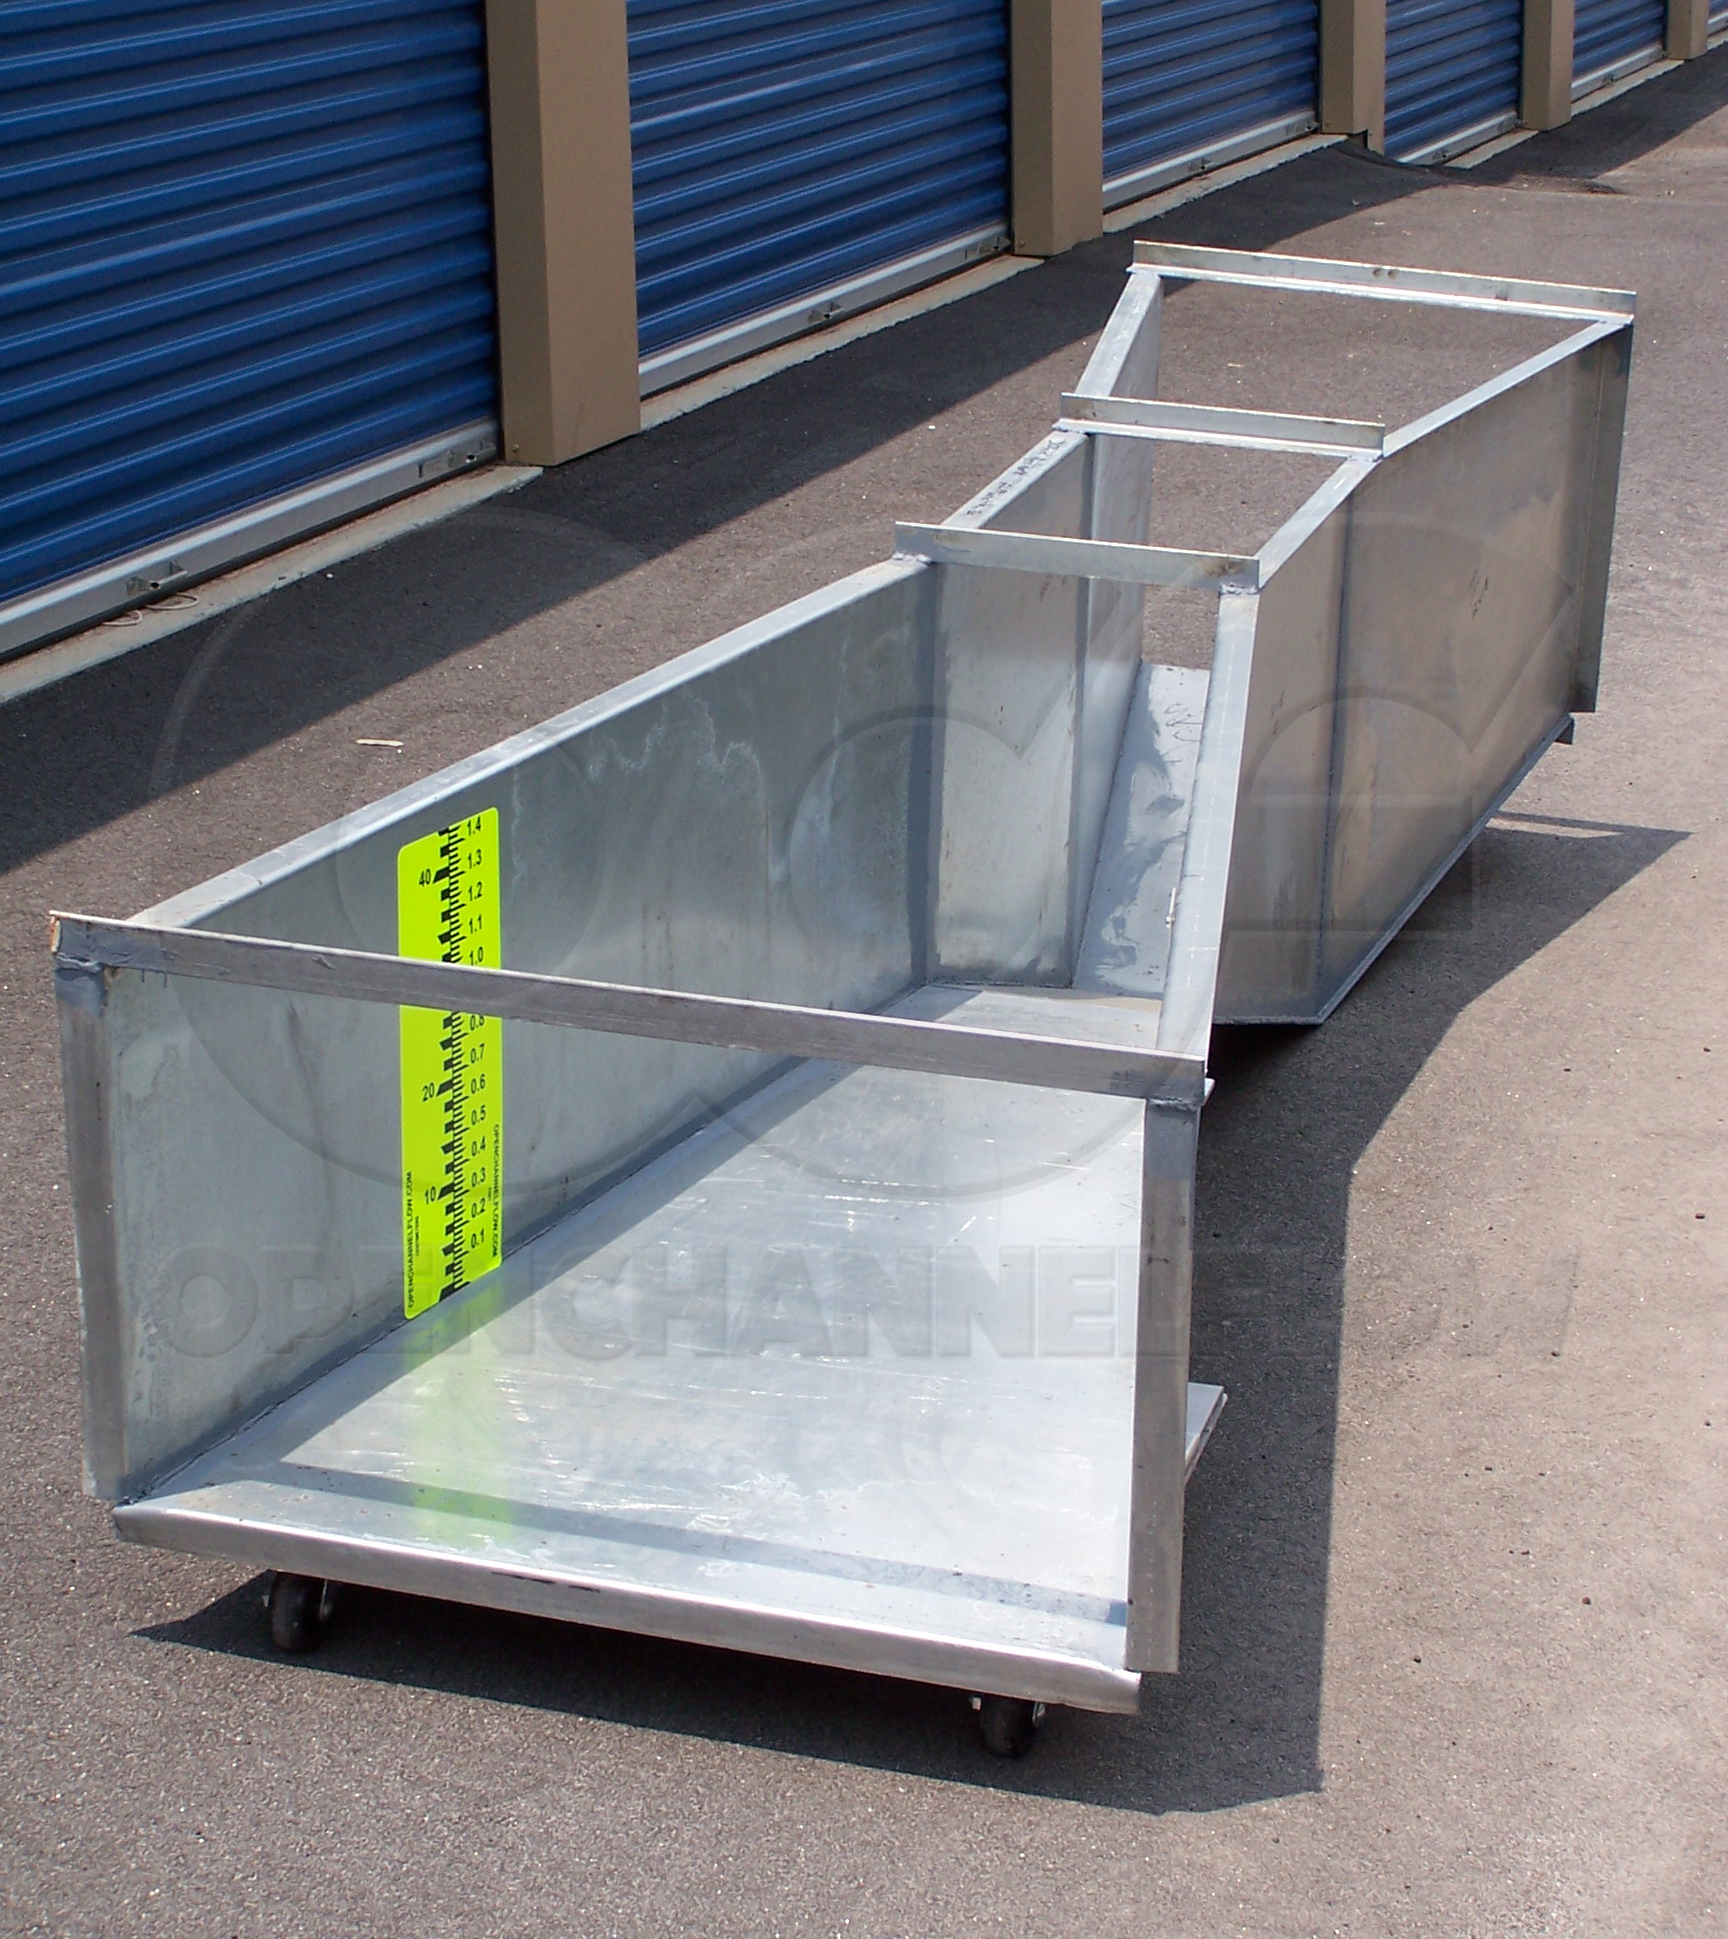
\includegraphics[width=0.75\linewidth]{parshallflume1}
    \caption{Parshall flume}
  \end{subfigure}
  \hspace{1cm}
  \begin{subfigure}[b]{0.4\linewidth}
    \includegraphics[width=\linewidth]{parshallflume2}
    \caption{Parshall flume with level sensor}
  \end{subfigure}
\end{figure}
		\subsubsection{Devices for Flow Measurement in Pipes}\index{Devices for Flow Measurement in Pipes}
					
					\begin{itemize}
						\item Venturi Tube:
							\begin{itemize}
								\item Measures the difference in pressure in the inlet and center section (throat)
								\item This pressure difference can then be mathematically converted to a flow rate.
								\item Works only when a pipe if flowing full
							\end{itemize}
						\item Magnetic Flow Meter (Magmeter):
							\begin{itemize}
								\item Magmeter is a pipe spool which has an electromagnetic coil surrounding it.  As the wastewater - a conducting material, flows through it, an electrical current is created proportional to the velocity of the conducting fluid (wastewater).
								\item Flow is automatically calculated by multiplying the velocity by the cross- sectional area of the pipe.
								\item Similar to the venturi meter, magmeter will read accurately only if the magmeter section of the pipe is flowing full and the wastewater is flowing through it at a certain minimum velocity.
							\end{itemize}
\begin{figure}[h!]
  \centering
  \begin{subfigure}[b]{0.4\linewidth}
    \includegraphics[width=0.9\linewidth]{magmeter1}
    \caption{Magmeter}
  \end{subfigure}
  \hspace{1cm}
  \begin{subfigure}[b]{0.45\linewidth}
    \includegraphics[width=\linewidth]{magmeter}
    \caption{Piping with magmeters}
  \end{subfigure}
\end{figure} 
					\end{itemize}
		\subsection{Grit Removal}\index{Grit Removal}
						\begin{itemize}
							\item Grit includes sand, gravel, cinder, eggshells, bone chips, seeds, coffee grounds, and large organic particles, such as food waste.
							\item Purpose of Grit removal:
								\begin{itemize} 
									\item to protect mechanical equipment from abrasion and abnormal wear 
									\item to reduce clogging caused by deposition of grit particles in pipes and channels, and 
				\item to prevent loading the treatment plant with inert matter that might interfere with the operation of treatment units such as anaerobic digester and aeration tanks.
			\end{itemize}
		\item Removal of organic material along with the grit is undesirable for two reasons:
			\begin{enumerate}
				\item It causes odor issues, and 
				\item Organic matter is a potential source of energy (digester gas)
			\end{enumerate}
		\item Grit Disposal: Grit removed is typically landfilled.
		\item Grit Volume:  The volume of grit collected measured in ft$^3$/MG.
		\item The rate of grit collection can range from 0.5 ft$^3$/MG to 30 ft$^3$/MG.
		\item Wastewater plants having a combined collection system must deal with much larger volumes of grit.
\end{itemize}
\subsubsection{Grit Removal Systems}\index{Grit Removal Systems}



			\begin{itemize}
			
					\item \noindent\textsc{Horizontal grit chambers:}

					\begin{itemize}
						\item These are rectangular channels 30 to 60 feet long and the water detention time is between 45 to 90 seconds
						\item Water passing through these channels is maintained at a relatively constant \hl{velocity of about 1 feet per second (fps)} which allows for the grit to settle while keeping the lighter organic material to stay in suspension and continue on into the primary clarifiers.
					\end{itemize}
	

						\item \noindent\textsc{Aerated grit chambers:}
	
					\begin{itemize}
						\item The 1 fps velocity is maintained by using aerators to create a rolling flow in the tank.
						\item Aeration is achieved using diffusers located on the bottom of one side of the grit chamber.
						\item Aerated grit chambers help create aerobic conditions in septic sewage. Aerobic conditions help improve the settleability of the sludge and increase both BOD and suspended solids removal in the primary clarifiers.
						\item Much larger and deeper than non-aerated units.
						\item The detention times are increased to 3 to 5 minutes.
					\end{itemize}

\begin{figure}[h!]
  \centering
  \begin{subfigure}[b]{0.46\linewidth}
    \includegraphics[width=0.8\linewidth]{HorizontalGritChamber}
    \caption{Horizontal grit chamber}
  \end{subfigure}
  \hspace{0.2cm}
  \begin{subfigure}[b]{0.5\linewidth}
    \includegraphics[width=0.8\linewidth]{AeratedGritChamber}
    \caption{Aerated grit chamber}
  \end{subfigure}
\end{figure} 					


						\item \noindent\textsc{Cyclonic/Vortex grit chamber:}


					\begin{itemize}
						\item The wastewater flows into a cylinder that tapers to a cone at one end.
						\item The flow whirls around the inside of the cylinder like a cyclone which causes the heavy grit to be slinged to the outside and it ultimately settles to the bottom from where it is withdrawn.
					\end{itemize}

\begin{figure}[h!]
  \centering
  \begin{subfigure}[b]{0.47\linewidth}
    \includegraphics[width=0.8\linewidth]{VortexGritChamber1}
    \caption{Vortex grit chamber design}
  \end{subfigure}
  \hspace{0.2cm}
  \begin{subfigure}[b]{0.43\linewidth}
    \includegraphics[width=0.8\linewidth]{VortexGritChamber}
    \caption{Vortex grit chamber installed}
  \end{subfigure}
\end{figure} 
	
\subsubsection{Grit Removal}\index{Grit Removal}		

		
			\begin{itemize}
				\item In the cyclonic/vortex grit chamber, the grit is scoured with water and is removed using pumps
				\item For the horizontal and aerated grit systems:
					\begin{itemize}
						\item Mechanical augers at the bottom of the grit chamber move the grit to one end of the tank where grit slurry pumps can pump it out of the tank to a grit separator.
						\item In some cases steep bottom slope is provided which will collect the grit at Central Point of Removal.
						\item Grit Removal is achieved by air pumps for small aerated grit chambers.
						\item Grit can also be removed by tubular conveyors, buckets type collectors, elevators screws conveyors, grit pumps and clam shell buckets
					\end{itemize}
			\end{itemize}
						\end{itemize}
%		\end{itemize}

\subsection{Flow Control}\index{Flow Control}	
	\begin{itemize} 
		\item Flow control is critical for grit removal, specifically for the horizontal and aerated grit chambers as excessive or inadequate velocities would lead to poor grit removal or cause excessive organic material settling along with the grit, respectively
		\item As the wastewater flows vary diurnally, it is important that velocity of the wastewater in the grit chamber should be maintained nearly constant - near 1 fps.
		
\begin{figure}[h]
    \includegraphics[width=\linewidth]{DiurnalFlow}\\
\begin{center}
Diurnal wastewater flow profile \\
\end{center}
%    \caption{Comminutor Schematic}
  \end{figure}		

		\item Constant velocity in a grit chamber is achieved by providing a \hl{proportional (Sutro) weir} at the outlet end of grit chamber.
		\item The shape of the opening between the plates of a proportional weir is made in such a way that the discharge is directly proportional to liquid depth in grit chamber resulting in maintaining a constant velocity of water even a the flow changes.
	\end{itemize}
\begin{figure}[h!]
  \centering
  \begin{subfigure}[b]{0.5\linewidth}
    \includegraphics[width=0.8\linewidth]{Sutroweir1}
    \caption{Proportional weir design}
  \end{subfigure}
  \hspace{1cm}
  \begin{subfigure}[b]{0.35\linewidth}
    \includegraphics[width=0.8\linewidth]{Sutroweir}
    \caption{Installed Proportional weir}
  \end{subfigure}
\end{figure} 

\subsection{Pre-aeration}\index{Pre-aeration}	
	\begin{itemize}
		\item Pre-aeration of the wastewater as part of the preliminary treatment may be provided as a separate process or increased detention time in an aerated grit chamber.
		\item Pre-aeration provides the follwoing benefits:
			\begin{itemize}
				\item freshens up wastewater by dissolving oxygen thereby reducing the wastewater septicity
				\item reduction of septicity allows for better settling - solids and BOD removal, in the following primary treatment process
				\item promotes grease separation which facilitates its removal during primary treatment
			\end{itemize}
	\end{itemize}
\subsection{Flow Equalization}\index{Flow Equalization}	

	\begin{itemize}
		\item Flow equalization involves storing a portion of peak flows for release during low-flow periods
		\item It prevents surges and allows for the operation of processes at design flows thus allowing for optimal physical, biological and chemical processes to take place.
		\item It results in saving capital costs as the processes may be built with a treatment capacity which is less than the peak flows
	\end{itemize}


\newpage
\section*{Chapter Assessment}
\begin{tcolorbox}[breakable, enhanced,
colframe=blue!25,
colback=blue!10,
coltitle=blue!20!black,  
title= Chapter Assessment]

\begin{enumerate}

\item A weir can be also be used for measuring flows\\

a. True \\
b. False 
\vspace{0.4cm}
\item The process of pre-aeration in no way influences the degree of settling in a primary clarifier\\
\vspace{0.4cm}
a. True \\
b. False 
\vspace{0.4cm}
\item Septic sludge has a low pH\\

a. True \\
b. False 
\vspace{0.4cm}
\item A Parshall flume measures the velocity of the influent flow\\

a. True \\
b. False 
\vspace{0.4cm}
\item  A barminutor frequently operates automatically. \\

a. True \\
b. False 

\vspace{0.4cm}
\item  A grit chamber with a faster flow velocity than recommended may allow appreciable organic matter to collect in the grit. \\

a. True \\
b. False 

\item Carryover of grit from the grit chamber may indicate the need to: \\

a. Increase rate of settled grit removal from the grit chamber.. \\
b. Decrease the operational depth of the channel. \\
c. Increase the flow to the primary clarifier. \\
d. Increase the air input to an aerated grit chamber. 

\vspace{0.4cm}
\item Characteristics that should be measured immediately after the sample is collected are: \\

a. Velocity and dissolved solids \\
b. Temperature, pH and DO \\
c. TSS and BOD \\
d. Hardness and alkalinity 

\vspace{0.4cm}
\item Flow proportionate composite samples are collected because: \\

a. The waste characteristics are continually changing \\
b. The flow is continually changing \\
c. The flow and waste characteristics are continually changing \\
d. This requires less time than grab samples \\
e. All of the above 

\vspace{0.4cm}
\item Grab samples are considered to be representative of the \\

a. Average daily condition at the sample location \\
b. Average daily condition in the system \\
c. System conditions for the two hours before and after the sample was taken \\
d. System condition at the time of the sample 

\vspace{0.4cm}
\item Grit is composed mostly of which of the following substances? \\

a. Grease \\
b. Colloidal solids \\
c. Rubber goods \\
d. Inorganics \\
e. Plastics 

\vspace{0.4cm}
\item Organisms in wastewater that are not harmful to humans but are indicators of diseases are: \\

a. Pathogens \\
b. Viruses \\
c. Coliform \\
d. Bacteria 

\vspace{0.4cm}
\item Which of the following pollutants would be removed to the extent in an efficiently operating grit chamber? \\

a. Egg shells \\
b. Seeds \\
c. Oils and grease \\
d. Sand \\
e. Fixed solids 

\vspace{0.4cm}
\item Proportional weirs usually are located at: \\

a. Immediately after the barscreens \\
b. Primary clarifiers \\
c. Aerobic digester scum boxes \\
d. Grit chambers \\
e. Inside the Parshall flume 

\vspace{0.4cm}
\item Which of the following process units is not usually considered to be a preliminary treatment unit? \\

a. Grit chamber \\
b. Bar screen \\
c. Comminutor \\
d. Bar rack \\
e. A meniscus 

\vspace{0.4cm}
\item  Which of the following would be included in the pretreatment unit? \\

a. preaeration \\
b. grit removal \\
c. screening \\
d. comminutor \\
e. all of the above 

\end{enumerate}
\end{tcolorbox}








\chapterimage{Week3Clarifier1.jpg} % Chapter heading image

\chapter{Primary Treatment}

%\section{Background}\index{Background}
\begin{itemize}
\item Synonyms:  primary treatment basin, primary clarifier, sedimentation basin, primaries, clarifier

	
		\item Primary treatment is after preliminary treatment and 				before secondary treatment
		\item Its two main objectives are: 
			\begin{itemize}
				\item Remove settleable solids
				\item Remove floatable solids
			\end{itemize}
		\item This is a physical process which relies on the physical 			properties - how heavy or light the suspended solids particles 		are to effect its separation
		\item Provides quiescent conditions for the influent 					wastewater for the heavier solids to settle and the lighter 			solids to float
		\item Removes settleable solids and floatables
		\item Settled solids are removed as sludge from the bottom of 			the clarifier
		\item Floatable solids including oil and grease are also 				removed, as scum from the surface\\
		\item The shape of the primary clarifier is either rectangular 		or circular
	
		\item Effective solids removal in the primary clarifiers will 			reduce the loading on the expensive secondary treatment 				process.
		\item The amount of solids removed during primary treatment 			may be enhanced by chemical addition - ferric or ferrous 				chloride as a coagulant and anionic polymer as the flocculant.  		This is called Chemically Enhanced Primary Treatment (CEPT).
\item \textbf{Typical Removal Rates:}\\
\begin{itemize}
\item \hspace{10mm} BOD removal – 25\% to 40\% and about 60\% with CEPT
\item \hspace{10mm} Suspended solids (SS) removal – 40\% to 60\% and about 75\% with CEPT
\item \hspace{10mm} Settleable Solids removal - $>$90\%
\end{itemize}
\end{itemize}
\clearpage
			\begin{center}
				\includegraphics[scale=0.9]{RectangularClarifier}\\
				Cross section of a Rectangular Clarifier\\

				\includegraphics[scale=0.1]{Blank}\\
				\includegraphics[scale=0.6]{CircularClarifierAI}\\
				Schematic cross section of a circular clarifier\\
				\includegraphics[scale=0.1]{Blank}\\
				\includegraphics[scale=0.5]{CircularClarifier3}\\
				Cross section of a circular clarifier\\
			\end{center}
				\includegraphics[scale=0.03]{Blank}\\


\section{Clarifier Zones}\index{Clarifier Zones}
				
\subsection{Inlet Zone}\index{Inlet Zone}		
				\begin{itemize}
					\item Inlet Zone is where the water enters the end 					of a rectangular tank, or the center of a circular 					or square tank.
					\item The Inlet Zone is designed to accomplish two 					objectives:
						\begin{enumerate}
							\item Reduce the velocity (dissipate 									energy in the incoming water)
							\item Distribute the flow evenly
						\end{enumerate}
					\item The inlet zone is equipped with a baffle.  					Inlet baffle reduces the velocity of the 							influent flow, prevent short circuiting which 							could cause solids being carried over to secondary 					treatment.  
						\begin{itemize}
							\item Circular tanks are equipped with a 								collar-type circular baffle that directs 								the water down as it enters the center of 								the tank.
							\item Rectangular tanks will have a plate 								baffle in front of the opening for the 									wastewater flow into the clarifier and 									another baffle just upstream - a 										perforated wall or a picket fence type 									baffle that spreads the water laterally 								across the inlet end of the tank.\\

\begin{figure}[h!]
  \centering
  \begin{subfigure}[b]{0.4\linewidth}
    \includegraphics[width=0.8\linewidth]{InfluentBaffle}
    \caption{Rectangular clarifier influent baffle}
  \end{subfigure}
  \hspace{1cm}
  \begin{subfigure}[b]{0.4\linewidth}
    \includegraphics[width=\linewidth]{CircularClarifierInfluentBaffle}
    \caption{Circular clarifier influent baffle}
  \end{subfigure}
\end{figure}	
	
%							\begin{center}
%							\includegraphics[scale=0.65]												{InfluentBaffle}\\
%							Rectangular clarifier influent baffle
%							\end{center}
%							
%														\begin{center}
%							\includegraphics[scale=0.65]												{CircularClarifierInfluentBaffle}\\
%							Circular clarifier influent baffle
%							\end{center}	
						\end{itemize}
				\end{itemize}

\subsection{Settling Zone}\index{Settling Zone}
			\begin{itemize}
				\item This is the largest portion of the tank where 					solids settle.
				\item The water velocity is reduced to 0.03-0.05 fps 					and the detention time is about 1.5 to 2 hours. 
				\item A clarifier is said to be short circuiting if 					the velocity of the water is greater in some sections 					than in others. The water passing through the higher 					velocity region will have a reduced detention time and 				settleable solids will carry through with this water 					as it goes over the weir.  Short circuiting is 							prevented by appropriately designing inlet baffles and weir plates (at the Outlet Zone).
			\end{itemize}

\subsection{Sludge Zone}\index{Sludge Zone}
			\begin{itemize} 
				\item Sludge zone is the bottom of the tank where the 					settled sludge collects and compacts.
				\item Sludge blanket depth should be measured and 						sludge should be removed at least every shift. A 						desirable blanket depth is typically established and 					the sludge pumping rate and regimen is established to 					maintain that desired sludge blanket level.
				\item Sludge rakes push the sludge to one end or the 					center of the tank so that it can be pumped out. 
				\item The rake drive is usually equipped with a torque 				indicator. A shear pin in the drive shaft will break 					to prevent damage to the gearbox or drive shaft. 
				\item Failure to remove sludge often enough will 						result in the sludge becoming septic releasing gas 						bubbles which hinders the sludge settling and also 						result in causing odor problems.
				\item The sludge from the primary clarifiers needs to 					be stabilized prior to its disposal.  The sludge 						(solids) from the primary clarifiers are mixed with 					the solids from the secondary treatment process and 					stabilized typically using a sludge digestion process. 
			\end{itemize}
\subsection{Skimming Zone}\index{Skimming Zone}

			\begin{itemize}
				\item The skimming zone is at the surface of the tank 					for scum removal
				\item Lighter solids and greases float to the surface 					of the clarifier as scum
				\item In Circular Clarifiers:  Floating matter is 						skimmed by a skimmer arm that is supported by the 						sludge rake and rotates with it around the tank. The 					floating matter is pushed over the beach plate by the 					wipers attached to the skimmer arm and into a scum box 				attached to the tank wall.\\
				\item In Rectangular Clarifiers:  The flights act as 							skimmers when the chain brings them to the surface and 				pushes the scum towards the scum troughs.  The scum 					trough may be designed to rotate (tip) periodically 					for the scum to flow in from the water surface.\\
							
				\item The scum collected from the primary clarifiers is sent 				to the digester for treatment along with the sludge 					removed.\\ 

				\vspace{1cm}
									\begin{center}
					\includegraphics[scale=0.06]{RotatingScumTrough}\\
					Rectangular clarifier scum trough\\
									\includegraphics[scale=0.02]{Blank}\\
				\end{center}	

				\item The flights in the rectangular clarifier are supported 				at the top by two parallel rails running along the 						length of the clarifier.\\
				\item There are wear plates (strips) installed at the 						clarifer bottom and on top of the rails to prevent the 				flights from riding directly on those surfaces.  To 					reduce friction, the flights have a wearing shoe 						attached.  
				\item Both the wear strip and the wearing shoe 					are disposable items and are replaced at fixed 							intervals.\\			
				\begin{center}
					\includegraphics[scale=0.07]												{RectangularClarifierComponents}\\
					Rectangular clarifier flights\\
				\end{center}						  
\end{itemize}
\subsection{Outlet Zone}\index{Outlet Zone}
			\begin{itemize}
				\item  This is the part of the clarifier where the 						settled water leaves to go to the secondary treatment 					processes.
				\item A channel called the effluent launder collects 					the effluent flow and directs it to the primary 						effluent piping. 
				\item Weirs are installed along the edge of the effluent launder channel to skim the water evenly off the surface of the tank. The most common type of effluent weir is a V-notch (or saw-tooth) weir.   A V-	notch weir is a plate that has notches, about 2-3 						inches deep, cut in it every 6-8 inches. If the weir is clean and level, it will remove water evenly all 					the way around the edge of the tank. This minimizes 					the upward velocities near the effluent launder and 					improves removal efficiencies. If the weir plate is not level or part of the weir becomes clogged with 				slime or debris, short-circuiting will result because 					more water will pass over the low side or the clean notches of the weir. Short-circuiting will cause poor 					settling and uneven sludge blanket buildup.
				\item In rectangular tanks the water leaves at the end 	opposite the influent.
												  
				\item In circular  tanks the water leaves at the edge of the tank.
				\item Also, in the circular clarifiers, an effluent baffle, just upstream of the weir, 					is installed to prevent floating solids from going 						over the weir.
\clearpage
				\begin{center}
					\includegraphics[scale=0.04]												{CircularClarifierComponents1}\\
					Circular clarifier skimmer arm, effluent baffle and v-notch weir\\
				\end{center}
				
			\vspace{0.8cm}
					\begin{center}
					\includegraphics[scale=0.07]												{RectangularClarifierWeir}\\
					Rectangular clarifier v-notch weir and launder\\
				\end{center}			
												  
			\end{itemize}

\clearpage
\section{Sludge Pumping}\index{Sludge Pumping}

	\begin{itemize}
		\item The sludge pumping from the clarifier must be adequate 			to prevent sludge from going septic. Septic sludges are much 			more difficult to thicken or de-water and cause odor issues. 
		\item Primary sludge normally averages 4-6\% solids. 
		Generally positive displacement pumps are used for primary 				sludge
		\item The pumping cycles must be designed to provide the 				thickest sludge possible.
		\item Excessive pumping or pumping without building solids to 			build up leads to pumping thinner (more water) sludge.
	\end{itemize}
\section{Design Parameters}\index{Design Parameters}
	\begin{itemize}
	\setlength\itemsep{1em}
		\item \textbf{Clarifier depth} – 8 to 12 feet
		\item \textbf{Hydraulic or surface loading}
			\begin{itemize}
			\item This rate is important to ensure good settleable 					solids removal efficiency
			\item It is expressed in terms of gallons per day per 					square foot (gpd/sq ft) of tank surface area
			\item Typical surface loading rate used for the design of 				primary clarifiers range between 300 to 1,400 gpd/sq ft, 				depending on the nature of the solids and the treatment 				requirements. Lower loading rates are frequently used in 				small plants in cold climates. In warm regions, low rates 				may cause excessive detention which could lead to 						septicity.
			\end{itemize}
	\end{itemize}
	
\section{Advance primary treatment (APT)}\index{Advance primary treatment (APT)}
Synonyms:  Advance primary treatment (APT), Chemically enhanced primary treatment (CEPT), Physical-chemical treatment (Phys-chem)
\subsection{Background}\index{Background}     
      
        \begin{itemize}
			\item Suspended solids present in wastewater are typically coated with bacterial slime and biological metabolic products which are negatively charged.  A significant portion of the suspended solids in wastewater do not settle easily due to gravity as:
				\begin{enumerate}
					\item the biological mass and the associated byproduct gases produced makes these particles buoyant, 
					\item the negative electrostatic charges on these particles cause these particles to be in constant state of motion due to electrostatic repulsion
				\end{enumerate}
			\item Advance primary treatment (APT) also known as Chemically enhanced primary treatment (CEPT) or Physical-chemical treatment (Phys-chem), involves chemical addition to the primary influent flow to enhance primary treatment TSS and BOD removal efficiencies
			\item a normal primary treatment process typically removes 40 to 60\% TSS and 25 to 40\% BOD.  TSS and BOD removal efficiencies of over 80\% and 60\% respectively, may be achieved by the use of APT.
			\item additional cost incurred for the chemical addition is in most cases is offsetted by the benefits which include:
				\begin{enumerate}
					\item by removing more BOD in the primary treatment cost associated with secondary treatment is reduced
					\item primary BOD is more easy to digest than the secondary biomass thus the digester gas production is increased and digested solids production is lowered thus saving biosolids hauling cost
					\item residual ferric chloride in the primary sludge provides H$_2$S and struvite control in the solids treatment processes  
				\end{enumerate}
		\end{itemize}
\vspace{0.4 cm}

\subsection{Process/mechanism}\index{Process/mechanism}    

APT is a two step chemical process:

\textbf{Coagulation}
				                \begin{itemize}
									\item Coagulation is the process by which the negative charge on these particles is reduced lowering the repulsion forces, by the use of a chemical such as ferric chloride and alum.\\
									\item The concentration of the coagulant required is dependent on the strength of the wastewater and the conveyance time of the wastewater.
									\item Typically the coagulant is added immediately after the grit chambers so the conveyance from the grit chambers to the primary clarifier provides adequate contact time and mixing.\\
									\item Parameters to ensure optimal coagulation are:
										\begin{itemize}
											\item Appropriate coagulation concentration
											\item Adequate mixing energy, and
											\item Adequate contact time
										\end{itemize}
									\item Overdosing the coagulant will adversely effect the settleability.
									\item Typical ferric chloride dosage for coagulation range from 12 to 22 mg/l.
								\end{itemize}
\textbf{Flocculation}
			                	\begin{itemize}
									\item Flocculation uses an anionic polymer - polymer which has negatively charged groups, to bridge the coagulated particles to a size which will settle in the primary clarifier.  
									\item The flocculated particles are prone to shearing thus the polymer is gently folded in with the coagulated wastewater just prior to entry into the primary clarifier
								\end{itemize}
					

\vspace{0.6cm}
\hspace{6.8 cm} \textbf{CEPT Schematic}\\
\vspace{0.6cm}
\hspace{1.5 cm}\includegraphics[scale=.13]{CEPTInitial} \hspace{0.7 cm}\includegraphics[scale=.13]{CEPTCoagulation}\hspace{0.7 cm}
\includegraphics[scale=.13]{CEPTFlocculation}\\
\hspace{0.8 cm} \textbf{Untreated Primary Inluent}\hspace{1.6 cm}\textbf{Coagulation}\hspace{2.8 cm}\textbf{Flocculation}\\	
	

\newpage
\section*{Chapter Assessment}
\begin{tcolorbox}[breakable, enhanced,
colframe=blue!25,
colback=blue!10,
coltitle=blue!20!black,  
title= Chapter Assessment]

\begin{enumerate}


\item  An Imhoff cone is often used to measure the effectiveness of primary sedimentation. \\

a. True \\
b. False \\


\item  An inadequate detention time in a primary clarifier would result in increased solids pumping to digesters \\

a. True \\
b. False \\


\item  A well-operated primary clarifier, will remove between 90 and 95 percent of the influent settleable solids. \\

a. True \\
b. False \\


\item  Baffles upstream of outlet weirs in primary tanks serve as a physical barrier to inhibit the loss of floating solids and grease. \\

a. True \\
b. False \\

\item  A device called an Imhoff cone is commonly used to measure settleable solids in: \\

a. Percent \\
b. mL/L \\
c. mg/L \\
d. ppm \\
e. SVI units \\


\item  An efficient primary clarifier is expected to remove what percent of the influent settleable solids? \\

a. 2 to 6 \% \\
b. 20 to 40 \% \\
c. 40 to 50 \% \\
d. 60 to 75 \% \\
e. 90 \% or better \\


\item  A primary clarifier does not have adequate detention time. Which of the following would result? \\

a. Decreased organic leading on secondary unit \\
b. Overloading of collector or flight drive motor \\
c. Increased solids pumped to digester \\
d. Low BOD removal \\
e. Reduced suspended solids in aeration tank. \\


\item  If the sludge depth in a secondary sedimentation tank is too high, what will happen? \\

a. Decreased turbidity in effluent. \\
b. Return activated sludge will have lower oxygen demand \\
c. Settleable solids from aeration tank will increase \\
d. Sludge may become septic \\


\item  Odors associated with septic sludge are usually caused by \\

a. A neutral pH \\
b. Inorganic matter \\
c. Short retention time in collection system \\
d. Active aerobic bacteria \\
e. Active anaerobic bacteria \\


\item  The main objectives of primary sedimentation are to remove: \\

a. Finely divided particles and dissolved organics \\
b. TDS and colloidal solids \\
c. BOD, COD, and SS \\
d. Settleable solids and floatables \\
e. Detritus and volatile organics \\


\item  The withdrawal of sludge from a primary clarifier should be slow in order to: \\

a. conserve electricity \\
b. prevent pulling too much water with the sludge \\
c. keep the BOD stabilized \\
d. not disturb the bacteria in the clarifier \\
e. protect the pump \\


\item  The withdrawal of sludge from a clarifier should be slow in order to: \\

a. protect the pump. \\
b. conserve electricity. \\
c. prevent the pulling of too much water with the sludge. \\
d. not disturb the bacteria in the digester. \\
e. avoid breaking the water seal in the digester. \\


\item  Which of the following terms refers to a hydraulic condition, typically indicated by billowing solids flowing over the effluent weir, where a portion of the flow through a clarifier experiences a much shorter detention time than the rest of the wastewater in the tank? \\

a. surging \\
b. shortcircuiting \\
c. overload \\
d. dispersion \\


\item  When wastewater enters a rectangular clarifier, it is often evenly dispersed across the entire width of the tank by means of: \\

a. a baffle. \\
b. a proportional weir. \\
c. a submerged launder. \\
d. a dome diffuser. \\
e. a hydraulic pump. \\


\item  Rectangular primary clarifiers have wooden or plastic flights, which are equipped with: \\

a. shear pins. \\
b. friction skirts. \\
c. wear shoes. \\
d. grease nipples. \\
e. sludge hinges. \\


\end{enumerate}
\end{tcolorbox}
	
	

% \documentclass{article}
% %\usepackage[english]{babel}%
% \usepackage{graphicx}
% \usepackage{tabulary}
% \usepackage{tabularx}
% \usepackage[normalem]{ulem}
% \usepackage{cancel}
% \usepackage{tikz} 
% \usepackage{pdflscape}
% \usepackage{colortbl}
% \usepackage{lastpage}
% \usepackage{multirow}
% \usepackage{enumerate}
% \usepackage[shortlabels]{enumitem}
% \usepackage{color,soul}
% \usepackage{pdflscape}
% \usepackage{hyperref}
% %\usepackage[table]{xcolor}
% \usepackage{rotating}
% \usepackage{amsmath}
% \usepackage{fixltx2e}
% \usepackage{framed}
% \usepackage{mdframed}
% \usepackage[T1]{fontenc}
% \usepackage[utf8]{inputenc}
% \usepackage{textcomp}
% \usepackage{siunitx}
% \usepackage{ifthen}
% \usepackage{fancyhdr}
% \usepackage{gensymb}
% \usepackage{newunicodechar}
% \usepackage[document]{ragged2e}
% \usepackage[margin=1in,top=1.1in,headheight=57pt,headsep=0.1in]
% {geometry}
% \usepackage{ifthen}
% \usepackage{fancyhdr}
% \everymath{\displaystyle}
% \usepackage[document]{ragged2e}
% \usepackage{fancyhdr}
% \everymath{\displaystyle}
% \usepackage{empheq}

% \usepackage[most]{tcolorbox}

% \usepackage{booktabs} % Required for nicer horizontal rules in tables


% \usepackage{enumitem}

% %\usepackage[table,xcdraw]{xcolor}
% \usetikzlibrary{arrows}
% \linespread{2}%controls the spacing between lines. Bigger fractions means crowded lines%
% %\pagestyle{fancy}
% %\usepackage[margin=1 in, top=1in, includefoot]{geometry}
% %\everymath{\displaystyle}
% \linespread{1.3}%controls the spacing between lines. Bigger fractions means crowded lines%
% %\pagestyle{fancy}
% \pagestyle{fancy}
% \setlength{\headheight}{56.2pt}

% \definecolor{myblue}{rgb}{.8, .8, 1}
% \newcommand*\mybluebox[1]{%
% \colorbox{myblue}{\hspace{1em}#1\hspace{1em}}}

% \chead{\ifthenelse{\value{page}=1}{\includegraphics[scale=0.3]{SCC}\\ \textbf \textbf Wastewater Constituents Analysis \& Laboratory Methods}}
% \rhead{\ifthenelse{\value{page}=1}{}{}}
% \lhead{\ifthenelse{\value{page}=1}{}{Wastewater Constituents Analysis \& Laboratory Methods}}
% \rfoot{\ifthenelse{\value{page}=1}{Module 1: WATR 048 - Spring 2019}{Module 1: WATR 048 - Spring 2019}}

% \lfoot{Shabbir Basrai}
% \cfoot{Page \thepage\ of \pageref{LastPage}}
% \renewcommand{\headrulewidth}{2pt}
% \renewcommand{\footrulewidth}{1pt}
% \begin{document}
% %\begin{empheq}[box=\mybluebox]{align}
% %a&=b\\
% %E&=mc^2 + \int_a^a x\, dx
% %\end{empheq}

% \newlist{steps}{enumerate}{1} % Defines "Steps" for enumerate as Step 1, Step 2 etc.
% \setlist[steps, 1]{label = Step \arabic*:} % Defines "Steps" for enumerate as Step 1, Step 2 etc.

% \setlist{nolistsep} % Reduce spacing between bullet points and numbered lists


%_______________________________________________________________________________________________________________________________________%
\chapterimage{IntroductionSecondaryTreatmentImage.jpg} % Chapter heading image

\chapter{Introduction to Secondary Treatment}
\begin{itemize}
\item While preliminary and primary treatment processes are designed primarily to remove solids from wastewater, secondary treatment is for the removal of organics.
\item Secondary treatment involves:
\begin{itemize}
\item biological conversion of the dissolved and suspended organics in wastewater into biomass, and
\item physical settling (separation) process where the solids including the biomass formed during secondary treatment is separated and removed from the treated wastewater.
\end{itemize}

\item With the removal of gross solids in the preliminary treatment followed by removable of settleable solids in the primary clarifiers and the removal of dissolved and suspended organics in the secondary treatment processes, the wastewater is considered treated.
\item Secondary treated wastewater is typically disposed or treated further for reuse or disposal (depending upon the end use/application and the NPDES permit stipulations).
\item The solids (biomass) removed from the secondary treatment is typically mixed with the solids from primary treatment and stabilized using a solids treatment process like sludge digestion prior to its disposal.
\end{itemize}
\vspace{1cm}

\textbf{Secondary treatment process incorporates one of the following three approaches:}


\section{Fixed film system}\index{Fixed Film System}	

\begin{itemize}
\item Here the microorganisms responsible for the treatment, grow on substrates such
as rocks, sand or plastic.
\item When the wastewater is spread over the substrate, the microorganisms up-take the organics present in the wastewater
\item Example of this secondary treatment process include trickling filters and rotating biological contactors\\
\end{itemize}

\section{Suspended Growth System}\index{Suspended Growth System}
\begin{itemize}
\item In this type of secondary treatment, the microbes are suspended in the
wastewater flow being treated. 
\item Air or oxygen is supplied to maintain an aerobic environment and to keep the microorganisms in suspension. 
\item Example of this secondary treatment approach include the activated sludge treatment process 
\end{itemize}

\section{Pond System}\index{Pond System}
Similar to the suspended growth, stabilization ponds are large man made bodies of water which treat wastewater using mainly natural processes including sunlight, algae and microorganisms.


% \documentclass{article}
% %\usepackage[english]{babel}%
% \usepackage{graphicx}
% \usepackage{tabulary}
% \usepackage{tabularx}
% \usepackage[normalem]{ulem}
% \usepackage{cancel}
% \usepackage{tikz} 
% \usepackage{pdflscape}
% \usepackage{colortbl}
% \usepackage{lastpage}
% \usepackage{multirow}
% \usepackage{enumerate}
% \usepackage[shortlabels]{enumitem}
% \usepackage{color,soul}
% \usepackage{pdflscape}
% \usepackage{hyperref}
% %\usepackage[table]{xcolor}
% \usepackage{rotating}
% \usepackage{amsmath}
% \usepackage{fixltx2e}
% \usepackage{framed}
% \usepackage{mdframed}
% \usepackage[T1]{fontenc}
% \usepackage[utf8]{inputenc}
% \usepackage{textcomp}
% \usepackage{siunitx}
% \usepackage{ifthen}
% \usepackage{fancyhdr}
% \usepackage{gensymb}
% \usepackage{newunicodechar}
% \usepackage[document]{ragged2e}
% \usepackage[margin=1in,top=1.1in,headheight=57pt,headsep=0.1in]
% {geometry}
% \usepackage{ifthen}
% \usepackage{fancyhdr}
% \everymath{\displaystyle}
% \usepackage[document]{ragged2e}
% \usepackage{fancyhdr}
% \everymath{\displaystyle}
% \usepackage{empheq}

% \usepackage[most]{tcolorbox}

% \usepackage{booktabs} % Required for nicer horizontal rules in tables


% \usepackage{enumitem}

% %\usepackage[table,xcdraw]{xcolor}
% \usetikzlibrary{arrows}
% \linespread{2}%controls the spacing between lines. Bigger fractions means crowded lines%
% %\pagestyle{fancy}
% %\usepackage[margin=1 in, top=1in, includefoot]{geometry}
% %\everymath{\displaystyle}
% \linespread{1.3}%controls the spacing between lines. Bigger fractions means crowded lines%
% %\pagestyle{fancy}
% \pagestyle{fancy}
% \setlength{\headheight}{56.2pt}

% \definecolor{myblue}{rgb}{.8, .8, 1}
% \newcommand*\mybluebox[1]{%
% \colorbox{myblue}{\hspace{1em}#1\hspace{1em}}}

% \chead{\ifthenelse{\value{page}=1}{\includegraphics[scale=0.3]{SCC}\\ \textbf \textbf Wastewater Constituents Analysis \& Laboratory Methods}}
% \rhead{\ifthenelse{\value{page}=1}{}{}}
% \lhead{\ifthenelse{\value{page}=1}{}{Wastewater Constituents Analysis \& Laboratory Methods}}
% \rfoot{\ifthenelse{\value{page}=1}{Module 1: WATR 048 - Spring 2019}{Module 1: WATR 048 - Spring 2019}}

% \lfoot{Shabbir Basrai}
% \cfoot{Page \thepage\ of \pageref{LastPage}}
% \renewcommand{\headrulewidth}{2pt}
% \renewcommand{\footrulewidth}{1pt}
% \begin{document}
% %\begin{empheq}[box=\mybluebox]{align}
% %a&=b\\
% %E&=mc^2 + \int_a^a x\, dx
% %\end{empheq}

% \newlist{steps}{enumerate}{1} % Defines "Steps" for enumerate as Step 1, Step 2 etc.
% \setlist[steps, 1]{label = Step \arabic*:} % Defines "Steps" for enumerate as Step 1, Step 2 etc.

% \setlist{nolistsep} % Reduce spacing between bullet points and numbered lists


%_______________________________________________________________________________________________________________________________________%
\chapterimage{TFChapterImage1.jpg} % Chapter heading image

\chapter{Trickling Filters}

\section{Theoretical Background}\index{Theoretical Background}
		
Trickling filter is a fixed film secondary treatment process wherein the organic content of the wastewater is removed using biological growth attached to an inert media such as lava rock or plastic\\			
\begin{itemize}
\item In a trickling filter, the wastewater is sprayed evenly on the surface of the media with a rotary type distributor with orifices
\item The wastewater percolates through the media bed, where it comes in contact with biological slime growth – zoogleal film (zooglea)
\item The aerobic biomass - bacteria, protozoa and other microoorganisms in the zooglea capture and consume the suspended and dissolved organics from the wastewater.
\item The microorganisms metabolize the organics and in the process produce more microbial mass resulting in increasing the thickness of the zoogleal layer.
\item The thickness of the zoogleal layer can only increase to a point until the wastewater flow – hydraulic load, shears the slime layer – “sloughs off” and is carried out as part of the effluent flow as sloughing.
\item The treated wastewater cascades from the bottom of the media into the underdrain system – lower portion of the TF comprised of columns which support the media base.  The underdrain has a sloping floor to direct the cascading water into a center channel .
\item The clarifier allows for the separation (settling) of the  of the solids (sloughed off material).  The settled solids is removed - typically pumped to a digester and the clarified effluent flows out of the clarifier.
\item The source of oxygen to support the aerobic growth is from the oxygen dissolved in the wastewater as it is sprayed over the media and from the air currents due to the downward flow of the wastewater and the temperature difference between ambient and the interior of the trickling filter.  Forced ventilation system may be designed as part of the trickling filter

\item Word trickling “filter” is a misnomer - no filtration is involved
\item Advantage includes process simplicity and lower costs
\item Disadvantage include BOD removal efficiency of only about 80-85%
\item The media may be rock, slag, coal, bricks, redwood blocks, molded plastic, or any other sound durable material.
\item The media depth ranges from about three to eight feet for rock media trickling filters and 15 to 30 feet for synthetic media.
\item The media needs to be uniformly sized and have adequate empty spaces (voids) to ensure maintaining aerobic condition necessary for the survival of biomass.  

\item Pre-fabricated (synthetic) media - similar to the one shown below, has an advantage over the "dumped" type media such as lava rock of providing a greater surface area per volume upon which the zoologeal film may grow while providing ample void space for the free circulation of air.

\item Sometimes, due to inadequate hydraulic loading, portions of the zoogleal layer may become too thick and oxygen cannot penetrate its full depth, causing odor issues.

\end{itemize}


\section{Trickling Filter Recirculation}\index{Trickling Filter Recirculation}

Recirculation - where a portion of the treated wastewater is returned back as the feed to the TF.  The parameter recirculation ratio is calculated to quantify the recirculation flow.  Recirculation ratio is a ratio of the recirculated flow - Q$_R$ to the influent flow Q$_I$. Recirculation ratios typically vary from 0.5 to 4.
\begin{center}
\includegraphics[scale=0.27]{TricklingFilterR1RecircRatioFormula}
\end{center}
Recirculation is beneficial for the following reasons:
\begin{itemize}
\item It improves the removal efficiency by increasing the contact time of the zoogleal layer with the wastewater
\item During low flows it prevents the trickling filter from drying out
\item It dilutes any toxic loadings
\item It promotes oxygen transfer and reduces ponding
\item The increased hydraulic loading promotes uniform sloughing, prevents ponding, improves ventilation through the filter and reduces potential for snail and filter fly breeding
\end{itemize}
\section{Operation of Multiple Trickling Filters}\index{Operation of Multiple Trickling Filters}

Multiple trickling filters can be operated in series or in parallel:\\
\begin{itemize}
\item Series operation in which the flow from one flows into the next.
\begin{center}
\includegraphics[scale=1]{TricklingFilterR1Series}
\end{center}  
\begin{itemize}
\item For high strength loading and for nitrification
\end{itemize}
\item Parallel operation in which the trickling filters that are operated side by side.
\begin{center}
\includegraphics[scale=1]{TricklingFilterR1Parallel}
\end{center}
\begin{itemize}
\item For winter operation - prevents freezing in the TF
\end{itemize}
\end{itemize}

\section{Parameters for monitoring and operating trickling filters}\index{Parameters for monitoring and operating trickling filters}



\begin{enumerate}
\item Hydraulic loading is expressed as gpd/$ft^2$
\item BOD Removal (\%)
\item Organic loading lbs BOD/day/ 1000 cu ft
\item Recirculation ratio
\end{enumerate}


\section{Classifying Trickling Filters}\index{Classifying Trickling Filters}			
Trickling filters are classified according to the hydraulic and organic loading applied to the  filter\\

\subsection{Low-rate filter}\index{Low-rate filter}

\begin{itemize}
\item The standard rate or low rate trickling filters (LRTF) are relatively simple treatment units that normally produce a consistent effluent quality even with varying influent strength
\item They are generally not provided with recirculation of effluent
\item Depending upon the dosing system, wastewater is applied intermittently with rest periods which generally do not exceed five minutes at the designed rate of waste flow. 
\item While there is some unloading or sloughing of solids at all times, the major unloadings usually occur several times a year for comparatively short Periods of time.
\end{itemize}

     Hydraulic loading is 25 - 100 gal/day/sq. ft\\
     BOD Removal (\%) 	50 – 80\%\\
     Organic loading is 5 - 25 lbs BOD/day/1000 cu ft\\

\subsection{High-rate filter}\index{High-rate filter}

\begin{itemize}
\item The most important element of a high-rate trickling filter is the provision where a part of the settled treated effluent is pumped to the PST or to the filter.  This is termed as \textbf{Recirculation}
\item High-rate filters are usually characterized by higher hydraulic and organic loadings than low-rate filters
\item The higher BOD loading is accomplished by applying a larger volume of waste per unit surface area of the filter.  \item As a result of the higher flow velocities a more continuous and uniform sloughing of excess zoogleal growth occurs
\end{itemize}

     Hydraulic loading is 100 - 1000 gal/day/sq. ft\\
     BOD Removal (\%) 	65 - 85\%\\
     Organic loading is 25 - 100 lbs BOD/day/ 1000 cu ft\\
			
\subsection{Roughing filter}\index{Roughing filter}

\begin{itemize}
\item Roughing filters are high rate type filters designed with plastic packing
\item In most cases roughing filters are used to treat wastewater prior to secondary treatment
\item One of the advantages of roughing filter is low energy requirement for BOD removal of high strength wastewaters as compared to activated sludge process because the energy required is only for pumping the influent wastewater and recirculation flows
\end{itemize}



\section{Trickling Filter Operational Issues}\index{Trickling Filter Operational Issues}

\subsection{Ponding}\index{Ponding}


If the voids in the media get plugged, flow can collect on the surface in ponds.
Correction:
spraying the surface with high pressure water stream
stopping a rotary distributor over the ponded area
hand-stir the media or open the voids
dose the filter with chlorine for several hours

\subsection{Odors}\index{Odors}


\begin{itemize}
\item Corrective measures should be taken immediately if foul odors develop
\item presence of foul odors indicates anaerobic conditions are predominant
\item Check the under drain system for obstructions or heavy biological growths
\item increase the recirculation rate to provide more oxygen to the filter bed and increase sloughing 
\item keep slime growths off of sidewalks and inside walls of the filter to reduce the odor
\end{itemize}

\subsection{Trickling Filter Flies - Psychoda}\index{Trickling Filter Flies - Psychoda}

\begin{itemize}
\item tiny, gnat-size filter fly, or Psychoda - primary nuisance insect
\item Correction methods include
\begin{itemize}
\item Increase recirculation rate
\item keep orifice openings clear
\item apply insecticides to filter walls
\item dose filter with chlorine
\item keep weeds and tall grass cut around filter
\end{itemize}
\end{itemize}


\subsection{Cold weather problems}\index{Cold weather problems}

\begin{itemize}
\item ice can form on the media of the filter
\item Correction methods include:
\begin{itemize}
\item decrease recirculation to the filter (influent is usually warmer than recycled flows)
\item construct wind screens
\item operate two-stage filters in parallel rather than in series
\end{itemize}
\end{itemize}



\newpage
\section*{Chapter Assessment}
\begin{tcolorbox}[breakable, enhanced,
colframe=blue!25,
colback=blue!10,
coltitle=blue!20!black,  
title= Chapter Assessment]

\begin{enumerate}
\item  Compared to activated sludge, trickling filters are sturdy work units not easily up set by shock loads. \\

a. True \\
b. False \\


\item  Ponding on the surface of trickling filters is almost always caused by plugging of the underdrains immediately below the point of ponding \\

a. True\\
b. False\\


\item  Zoogleal mass sheared of from the trickling filter media and carried out as part of the effluent flow is termed as sloughing \\

a. True \\
b. False \\


\item  For multiple trickling filter operation, the parallel mode is more suitable than the series mode for treating influent wastewater with a high BOD content \\

a. True \\
b. False \\


\item  Synthetic /pre-manufactured media used in the biofilter has the advantage of providing a greater surface area per volume upon which the zoologeal film may grow while providing ample void space for the free circulation of air. \\

a. True \\
b. False \\

\item  A good reason to run a trickling filter in the parallel mode of operation is: \\

 a. When the weather is warm \\
 b. When the BOD loading is high \\
 c. When the BOD loading is low \\
 d. To prevent filter flies \\


\item  A pan test should be done monthly on a trickling filter to: \\

 a. Check oil quality in the distributor bearing \\
 b. Check sewage distribution on filter \\
 c. To check flow rates through the media \\
 d. All the above \\
 e. None of the above \\


\item  A problem associated with trickling filters is \\

 a. Bulking \\
 b. Protozoans \\
 c. Ponding \\
 d. Liquefaction \\


\item  A trickling filter or activated sludge process causes nitrification. which is \\

 a. Conversion of nitrogen to nitrate \\
 b. Conversion of nitrogen to ammonia \\
 c. Conversion of nitrate to nitrogen \\
 d. Conversion of ammonia to nitrate and nitrite nitrogen \\


\item  Most common trickling filter operational control method is: \\

 a. Sloughing control \\
 b. Recirculation \\
 c. Sludge removal \\
 d. Distributor arm speed \\
 
 \end{enumerate}
 \end{tcolorbox}
\chapterimage{Week5Ponds.jpg} % Chapter heading image

\chapter{Stabilzation Ponds}
% Chapter heading image

\begin{itemize}
\item Stabilization ponds and lagoons are bodies of water which treat wastewater using mainly natural processes including sunlight, algae and microorganisms for treating wastewater\\
\item While ponds are shallow and man-made, lagoons are bodies of water confined within natural boundaries.\\
\end{itemize}


\section{Advantages of ponds}\index{Advantages of ponds}	

\begin{itemize}	
\item Cheap to build and operate
\item Low maintenance and electrical costs
\item Do not require highly trained operational personnel
\item Provide treatment that can be equal to some secondary treatment processes and have fewer sludge handling issues.\\
\end{itemize}


\section{Disadvantages of ponds}\index{Disadvantages of ponds}	
\begin{itemize}	
\item Land intensive
\item Effluent quality varies with seasonal temperature changes
\item Suspended solids levels that can create regulatory problems.
\item System upsets almost always result in odor problems and recovery times may be weeks or months.
\item Not appropriate for colder climates
\end{itemize} 

\section{Types of Ponds}\index{Types of Ponds}	

\subsection{Anaerobic Ponds}\index{Anaerobic Ponds}	

\subsubsection{Anaerobic Ponds}\index{Anaerobic Ponds}	

\begin{itemize}	
\item Typically for treating raw sewage
\item These are deep - 10-14 feet treatment ponds which rely primarily on anaerobic bacteria to break down the organic waste.
\item Designed for BOD removal.
\item High strength wastewater may be treated.
\item Organic matter is broken down releasing releasing methane, carbon dioxide and odorous gases including hydrogen sulfide. 
\item Most of the decomposition is accomplished by acid forming bacteria. 
\item The pH in these lagoons is usually below 6.5. 
\item They are total retention and do not have an effluent discharge. 
\item The anaerobic pond must be de-sludged approximately once every 2 to 5 years
\item Organic loading of 200-1000 lbs. $BOD_5$ per acre per day
\end{itemize}

\subsection{Facultative Ponds}\index{Facultative Ponds}	

\begin{itemize}
\item The depth of facultative ponds is about 4-7 feet which is in-between the depths of anaerobic ponds (10-14 feet) and aerobic ponds 3 feet)
\item The uper layer of facultative pond is aerobic, and bottom layer is mostly anaerobic.
\item Facultative bacteria are responsible for most of the treatment that occurs in these ponds.  Facultative bacteria are bacteria which can live under both aerobic and anaerobic conditions.
\item The algae that grow in the pond are critical to the successful stabilization of the organic load. 
\item The algae will take in carbon dioxide ($CO_2$) and, through photosynthesis, use it to create sugars and release dissolved oxygen ($O_2$) that is used by the aerobic bacteria. Facultative lagoon levels should always maintain at least 4 feet of water in the pond.
\item Typically for secondary treatment - BOD removal
\item 15-50 lbs $BOD_5$ per acre per day.
\item Unused CO$_2$ will react with water to form carbonic acid - which would reduce the pH unless consumed
\item Sludge removal need is rare.  Sludge can be removed by using a raft-mounted sludge pump or by draining and dewatering the pond and removing the sludge with a front-end loader.
\end{itemize} 

				\begin{sidewaysfigure}
\begin{center}
\includegraphics[scale=0.8]{StabilizationPond}\\
Facultative pond schematic
\end{center}
				\end{sidewaysfigure}
				
\subsection{Aerobic Stabilization Ponds}\index{Aerobic Stabilization Ponds}
	
Aerobic stabilization ponds are also known as: \hl{maturation}, \hl{polishing} or \hl{finishing} Pond
\begin{itemize}
\item Contain disssolved oxygen throughout entire depth of the pond.
\item Treatment is accomplished through the stabilization of organic wastes by aerobic bacteria and algae.
\item Typically for tertiary treatment
\item Designed for pathogen removal
\item Shallow - only about 3 feet deep. 
\item They are most often the final cells in a multi-staged pond system
\item They are also used as polishing ponds for tertiary treatment of trickling filter plant effluent.
\item Usually the effluent is directed into a second pond where the sludge can settle 
\item Their shallow depth allows sunlight to penetrate to the bottom of the pond to encourage algae growth and aerobic conditions throughout the pond 
\item The low solids loading found in these tertiary treatment applications means that these ponds normally have no sludge zone
\item These ponds may be mechanically aerated 
\item Aerobic polishing ponds are designed for 15-20 pounds BOD/acre/day
\item Aerobic ponds are typically designed for pathogen removal
\item Aerobic lagoon levels should always maintain at least 18 inches of water in the pond
\end{itemize}



\section{Ponds Operations and Maintenance}\index{Ponds Operations and Maintenance}

\begin{itemize}
\item Ponds and lagoons are designed as continuous discharge, controlled discharge, or no discharge.
\begin{itemize}
\item In controlled discharge ponds the wastewater is held for long periods of time before discharging. 

\item No-discharge ponds the inflow rate needs to be equal or exceed the rates of evaporation and/or percolation. 
\end{itemize}
\item Short-circuiting in a pond may be caused by poor design of inlet and outlet piping arrangements or by uncontrolled growth of water weeds.
\item Stagnant water will breed mosquitoes and can result in anaerobic conditions developing that can cause odor issues 
\item Dikes need to be maintained
\item Aquatic plants and weeds must be removed from the water. 
\item Reeds will create stagnant areas along the edge of the pond and need to be removed
\item To start a new pond, two feet of water is typically added prior to fresh starting wastewater feed. 
\item Sodium nitrate can be used to help recover from an odor-causing upset. The nitrates ($NO_3$) will provide a source of chemically bound oxygen for the bacteria to use instead of dissolved oxygen.
\item Scum control may be required
\end{itemize}





\newpage
\section*{Chapter Assessment}
\begin{tcolorbox}[breakable, enhanced,
colframe=blue!25,
colback=blue!10,
coltitle=blue!20!black,  
title= Chapter Assessment]

\begin{enumerate}

\item  Organic loading to a stabilization pond is always calculated by knowing the pounds of BOD applied per 1.000 cubic feet of pond volume per day.\\


a. True \\

b. False \\


\item  An abundance of aquatic plant growth in and around the edge of a facultative pond provides more surface area for biologic activity and increases treatment capacity.\\


a. True \\

b. False \\


\item  Facultative ponds are anaerobic on the bottom and aerobic near the surface.\\


a. True \\

b. False \\


\item  The best time of the year to initiate operation of a new facultative pond is during the coldest months of the year.\\


a. True \\

b. False \\


\item  Ponds that contain an aerobic top layer and an anaerobic bottom layer are called facultative ponds.\\


a. True \\

b. False \\


\item  One short-term corrective measure for an overloaded facultative pond might be to add:\\


a. copper sulfate . \\

b. sodium sulfide. \\

c. ammonium sulfide . \\

d. sodium nitrate. \\

e. potassium chloride. \\


\item  Photosynthesis is an essential part of the biological activity associated with:\\


a. Activated sludge \\

b. Trickling filters \\

c. Oxidation ditches \\

d. Aerobic digesters \\

e. Sewage lagoons \\


\item  During the process of algal photosynthesis:\\


a. Chlorophyll converts sunlight into energy for growth. \\

b. Algae produces oxygen \\

c. Algae converts CO2, NH3, and PO4, into additional algae cells \\

d. All of the above \\


\item  pH of the facultative pond will be the highest\\


a. during daytime when the consumption of CO2 is the highest \\

b. during daytime when the consumption of CO2 is the lowest \\

c. during nighttime when the production of CO2 is highest \\

d. during nighttime when the production of CO2 is lowest \\


\item  A lagoon operator collects a sample of effluent at 2:15 pm. on a sunny July day and tests it. for dissolved oxygen. The dissolved oxygen is 22 mg/1 and the pH is 9.2.  The lagoon has a green color. Effluent suspended solids have been running at 75 mg/1.  The operator should \\


a. Do nothing. The conditions described are normal. \\

b. Apply algaecide to the lagoon to kill the algae. \\

c. Drawdown the lagoon to eliminate excess DO. \\

d. Isolate cell. \\


\item  Algae in a stabilization pond is most likely to: \\


a. consume oxygen during daylight hours. \\

b. decrease effluent TSS during the day. \\

c. change the pH throughout the day. \\

d. increase oxygen at night. \\

e. None of the above. \\


\item  Algae in a stabilization pond is most likely to: \\


a. consume oxygen during daylight hours. \\

b. decrease effluent TSS during the day. \\

c. change the pH throughout the day. \\

d. increase oxygen at night. \\

e. None of the above. \\


\item  An operator cannot maintain adequate water levels in one of the ponds. What will cause this to happen? \\


a. The pond is hydraulically overloaded. \\

b. The pond seal leaks. \\

c. The flow control structure leaks. \\

d. The flow control structure does not split the flow evenly. \\


\item  A properly designed and operated wastewater stabilization pond will remove \rule{1.5cm}{0.3mm} percent BOD. \\


a. 40\%-60\%. \\

b. 60\%-70\%. \\

c. 70\%-80\%. \\

d. 80\%-90\%. \\


\item  At night algae in a conventional lagoon will: \\


a. Cease to produce oxygen \\

b. Consume oxygen \\

c. Produce less oxygen \\

d. Increase the pH of the lagoon contents \\


\item  At what time of day is the dissolved oxygen content highest in a lagoon? \\


a. 3 a.m. \\

b. 7 a.m. \\

c. 9 a.m. \\

d. 3 p.m. \\
\end{enumerate}
\end{tcolorbox}
\input{BassettWWActivatedSludge.tex}
\input{BassettWWNutrientRemoval.tex}
\input{BassettWWSolidsTreatmentOverview.tex}
\input{BassettWWBiosolidsRegulations.tex}
\chapterimage{Chapter14.jpg} % Chapter heading image

\chapter{Sludge Thickening}

			Prior to the sludge stabilization process such as anaerobic digestion, the solids content of the sludge is increased by utilizing an appropriate thickening process.\\
			Notes:\\
			1) There is an upper limit of the solids concentration that can be effectively treated as increasing the solids concentration reduces its ability to be mixed and pumped easily. Digesters can effectively treat sludges with upto about maximum 7\% - 9\% solids.\\
			2) If a 5000 mg/l (0.5\%) sludge is thickened to 5\% solids concentration - it will reduce the volume of sludge by 90\%\\

\section{Advantages of sludge thickening}\index{Advantages of sludge thickening}

		\begin{itemize}
			\item Improved digester performance due to a lower volume of sludge
			\item Capital Cost savings associated with less digester volume requirements
			\item Operational costs savings - for sludge heating and mixing
		\end{itemize}
        
\section{Sludge thickening methods}\index{Sludge thickening methods}

		\begin{enumerate}
			\item Gravity thickener - more suitable for primary sludge
			\item Dissolved air floatation thickener - more suitable for lighter, fluffier floc such as the secondary sludge.
		\end{enumerate}
\section{Gravity thickener}\index{Gravity thickener}
The gravity thickener is designed and operated similar to a circular primary and secondary clarifier.
\begin{center}
\includegraphics[scale=0.45]{GravityThickener}\\
\vspace{1cm}
\includegraphics[scale=0.45]{ThickenerGravityThickener}
\vspace{1cm}
\end{center}
\subsection{Principles of gravity thickener operations}\index{Principles of gravity thickener operations}
   
\begin{itemize}
\item Upon entering the tank from the center, the sludge solids settle under the influence of gravity and these settled solids accumulate in the bottom of the gravity thickener as the sludge blanket.  As the sludge becomes thicker it helps squeeze out more water from the sludge increasing the sludge solids content.
\item Typical solids loading rates of a gravity thickener used for thickening primary sludge is 20-30 lbs TS/day-ft$^2$
\item A picket fence-like mechanism which is attached to the bottom sludge rake arms is primarily to release entrapped gases.  The sludge rake arms rotate at a very slow speed to ensure that it does not cause turbulenece causing the sludge to rise.  The sludge is gently raked towards a sump in the center, from where the solids are withdrawn.  The sludge rake encounter much higher torques than the typical primary clarifier rake, and is therefore designed to be more stronger and heftier. 
\item The thickened solids are drawn-off at regular intervals and the liquid fraction is decanted from the top and returned to the primary clarifier.  The typical sludge concentration factor is about 2.
\item The sludge blanket is kept about three feet.  
\item The sludge blanket depth is typically maintained so that the sludge does not turn septic and the effluent is relatively clear and free of solids.  
\item Sludge Volume ratio (SVR) provides a means of regulating the detention time of sludge within the blanket of the thickener
\item SVR is defined as the volume of the sludge blanket divided by the daily volume Of sludge pumped from the thickener. 
\item SVR is a relative measure of the average detention time of solids in the thickener and is calculated in days.
\item Typical SVRs for primary sludge range from 0.5 - 2 days.
\item Scum is removed from the top using a separate scum removal mechanism.

\item Chemical additives may be utilized to enhance settling and control odors.
\end{itemize}

\subsection{Elements of a gravity thickener}\index{Elements of a gravity thickener}

\begin{itemize}
\item center feed column and baffle\\
\item drive assembly\\
\item scum removal system\\
\item thickened sludge pump\\
\item sludge rake with pickets\\
\item effluent weir\\
\item sludge hopper and pump\\
\end{itemize}

\subsection{Gravity thickener operational parameters}\index{Gravity thickener operational parameters}

\begin{itemize}
\item type and quality of sludge\\
\item hydraulic or surface loading rate (GPD/$ft^2$/day)\\
\item solids loading rate (lbs/$ft^2$/day)\\
\item sludge volume ratio - sludge detention time\\
\item solids and hydraulic loading rates, and\\
\item quantity and characteristics of the polymer used\\
\end{itemize}

\section{Dissolved air floatation thickener (DAFT)}\index{Dissolved air floatation thickener (DAFT)}
Opposite to the principle of the gravity thickener where the thickened sludge forms a blanket at the bottom, in the DAFT the thickened sludge forms a blanket on the top surface.  Primary sludge is not generally suitable for thickening using DAFT as its solids are heavier and do not float easily. The WAS from the secondary clarifier which typically has a solids content of about 0.5\% to 0.8\% is thickened to about 4\% to 6\% concentration – thickened WAS (TWAS) using the DAFT.

\begin{center}
\includegraphics[scale=0.3]{DAFTOutside}\\
\vspace{1cm}
\includegraphics[scale=0.4]{DAFT}

\end{center}

\subsection{Principles of DAFT operations}\index{Principles of DAFT operations}

\begin{itemize}
\item WAS is conditioned with cationic polymer and introduced into the DAFT.  DAFTs typically operate at a solids loading rate of 1-2 lbs TSS/hr-ft$^2$.  Polymer feed ranges from 5-15 lbs of polymer/ton of the WAS (feed) solids.
\item Recycled water from the DAFT is pressurized with air in the saturation tank and mixed with polymer treated WAS as it is released at the bottom of the DAFT using the Back Pressure Control Valve.  
\item The dissolved air from the pressurized water is released as minute air bubbles rises upwards carrying with it the polymer flocculated sludge to the surface.  Adequate quantity of air is required to float the WAS solids.  Air:Solids ratio is one of the key operating and control parameter.  Typical air:solids ratios in a DAFT are between 0.03 - 0.05 lb air per lb TS. PS: Density of air used for air:solids ratio calculations - 0.075 lb air/ft$^3$ air - this value is given as part of the problem. 
\item The thickened solids floating on the top are scrapped off the surface of the DAFT by flights into the TWAS sump from where it is pumped to the digesters. The subnatant - water below the solids, part of it is used for the air pressurization in the saturation tank and the remaining is the underflow, which is returned back to the influent flow.
\item The flight speed is critical to the DAFT performance.  Fast flight speed would limit the thickness and density of the sludge blanket while slower flight speed would result in the thickened solids layer getting more dense and thick.  Excessively thick solids layer could result in the solids escaping through the underflow.  

\end{itemize}

\subsection{Elements of a DAFT}\index{Elements of a DAFT}

\begin{itemize}
\item pressurization or saturation tank 
\item thickened sludge skimmer with drive assembly
\item polymer dosing and injection system
\item thickened sludge pump
\item back pressure control valve
\item underflow removal
\item recycled flow system
\end{itemize}

\subsection{DAFT operational parameters}\index{DAFT operational parameters}

\begin{itemize}
\item saturation pressure
\item solids loading rate (lbs TSS/hr-$ft^2$)
\item hydraulic loading rate (GPD/$ft^2$/day)
\item feed solids concentration
\item detention period
\item air-to-solids ratio (lb air: lb solids)
\item type and quality of sludge
\item flight speed
\item solids and hydraulic loading rates, and
\item quantity and characteristics of the polymer used (lbs polymer/dry ton solids)
\end{itemize}


\newpage
\section*{Chapter Assessment}
\begin{tcolorbox}[breakable, enhanced,
colframe=blue!25,
colback=blue!10,
coltitle=blue!20!black,  
title= Chapter Assessment]

\begin{enumerate}


\item  In a gravity thickener the depth of the sludge is kept minimal (<six inches) to avoid solids going over the effluent weir \\

a. True \\
b. False \\

\item  Sludge thickening is primarily conducted to reduce costs associated with biosolids hauling\\


a. True \\
b. False \\


\item  Gravity thickener is commonly used for sludge dewatering \\

a. True \\
b. False \\

\item  Sludge thickening is primarily conducted to reduce costs associated with biosolids hauling \\

a. True \\
b. False \\
\item A DAF thickener has effluent solids of 55 mg/L and float solids of 2.0\%. Solids loading and polymer dosing is in the normal range. This data likely indicates: \\

a. This unit is operating normally \\
b. Too low air to solids ratio \\
c. Float blanket too thick \\
d. Flight speed too fast \\
e. Flight speed too slow \\

\item  An air flotation thickener will produce a thin float if: \\

a. Flight speed too high and skimmer wiper not adjusted properly \\
b. Excessive air/solids ratio and polymer dosages too low \\
c. High dissolved oxygen and flight speed too low \\
d. Polymer dosages too high and unit overloaded \\

\item  An increase in the pool depth of a scroll-type centrifuge: \\

a. would not affect the moisture content of the cake. \\
b. would produce a drier cake \\
c. would produce a wetter cake, but produce a greater solids recovery. \\
d. would not affect either solids recovery, nor cake moisture content. \\
e. would require an increase in the cationic polymer dosage. \\

\item  A sludge thickened from 1\% to 4\% solids will be reduced in volume by how much? \\

a. no more than 4\% of original volume \\
b. approximately 17\% of original volume \\
c. approximately 25\% of original volume \\
d. more information is needed \\

\item  Gravity thickeners, compared to DAFs, are best suited to: \\

a. Thickening primary sludge. \\
b. Thickening waste activated sludge. \\
c. Controlling sulfide odors. \\
d. Removing filamentous bacteria. \\
e. Provide highest concentration sludge. \\

\item  Which of the following is not the main reason for thickening sludge \\

a. Improved digester performance due to a lower volume of sludge \\
b. Cost savings in the construction of new digestion facilities \\
c. Reduction in anaerobic digestion heating requirements since less water has to be heated \\
d. Reduce costs of biosolids hauling \\
\end{enumerate}
\end{tcolorbox}
\input{BassettWWSolidsStabilizationDigestion.tex}
\chapterimage{Dewatering.jpg} % Chapter heading image

\chapter{Solids Dewatering}



        \begin{itemize}
        	\item Dewatering, like thickening does not treat the sludge but it allows for a reduction in sludge volume by removing water.  
        	\item Thickening achieves about 10\% or less solids content while dewatering is typically for increasing the solids content to between 15 to 30 percent. 
        	\item Sludge is dewatered to make it easier to handle and to reduce costs associated with elements related to accomplishing the end objectives with the sludge – land application, composting, drying, incineration or landfill.
        	\item Dewatering involves conditioning the sludge with a polymer and subjecting it to a physical process such as belt filter press or centrifuge to remove the water. 
        	\item Reasons for sludge dewatering are:
				\begin{itemize}
					\item Critical for sludge treatment options such as sludge drying and incineration.
					\item Reduction in the weight of solids to be hauled – reducing hauling cost.
					\item Reduction in the volume of sludge that needs to be handled
				\end{itemize}
			\item More common sludge dewatering methods include:
				\begin{enumerate}
					\item Belt Filter Press 
					\item Centrifuge
				\end{enumerate}
			\item These are both mechanical methods and involve physically removing free water
			\item Both these methods involve conditioning of sludge with a cationic polymer which flocculate the solids - separating it from the water

		\end{itemize}

\section{Belt Filter Press}\index{Belt Filter Press}

The belt filter press dewaters sludge by squeezing polymer conditioned sludge between a pair of belt filter fabric as these belts pass through a system of rollers. Belt filter press produces a dewatered product typically between 12\% to 35\% solids content.


		\begin{center}
		\includegraphics[scale=0.5]{BeltFilterPress}\\
		\vspace{1cm}
		\includegraphics[scale=0.28]{BeltPressPicture}\\
		Belt Filter Press
		\end{center}

\subsection{Principles of belt filter press operations}\index{Principles of belt filter press operations}
					\begin{itemize}
						\item Belt filter press utilizes two endless, porous belts (generally 0.7 to 3 meter wide) made from a synthetic material
						\item Polymer flocculated sludge is first introduced on the horizontal \hl{gravity zone} of the press where free water is removed from the sludge by chicane assisted gravity filtration through the porous belt press fabric.
						\begin{center}
						\includegraphics[scale=0.2]{Chicanes}\\
						Gravity Zone - Chicanes
						\end{center}
						\item From the gravity zone, the sludge enters the \hl{low pressure zone (wedge zone)} in which the sludge is prepared for the upcoming \hl{high-pressure zone} by evenly distributing the solids across the belt and gradually applying pressure
						\item In the high pressure zone the sludge is sandwiched between two belt press fabrics. As the belts with the sandwiched sludge passes over and under 6 to 12 tensioning rollers which progressively decrease in diameter.  The applied pressure squeezes the water out from the sludge and is removed through the porous fabric.
						\item The filtrate is returned back to the front of the plant.
						\item The belts are washed continuously as they pass over \hl{wash boxes}.  The wash boxes are equipped with rotating brushes and water sprays and are primarily for keeping the belt press fabric pores open so water could easily filter through.  
						\item Improper polymer dosage and excessive hydraulic loading can lead to a wetter sludge cake.
						\item The belts are operated at speeds that commensurate with the rate of solids loading and the type of sludge being dewatered. Lower belt speed would allow for better water removal.  However, if if the belts speed is below the threshold for that particular sludge, belt press \hl{washout}, which is characterized by sludge flowing over the sides of the belt can occur .  Thus, the best belt speed is the slowest speed the belt can be operated without causing washout.
						\item The belts can be blinded - loose its porosity causing the water to stagnate/cause washout and not filter through, if excessive polymer is used or due ineffective belt washing.
						\item \hl{Solids capture rate} and \hl{Percent cake solids} produced are the most important belt press efficiency measurement parameters
					\end{itemize}
\subsection{Elements of the belt filter press}\index{Elements of the belt filter press}


 
						\begin{itemize}
							\item belts
							\item wash boxes
							\item guiding and tensioning rollers
							\item chicanes 
							\item doctor blades
							\item drive motor
							\item hydraulic unit
							\item polymer injection and mixing system
						\end{itemize}

\subsection{Belt press operational parameters}\index{Belt press operational parameters}


						\begin{itemize}
							\item belt filter width
							\item belt filter speed
							\item hydraulic loading
							\item belt tension
							\item washout
							\item filtrate quality
							\item solids capture rate
							\item polymer dosing rate (lbs polymer/dry ton solids)
							\item solids and hydraulic loading rates, and
							\item quantity and characteristics of the polymer used
						\end{itemize}

\section{Centrifuge}\index{Centrifuge}
			The centrifuge dewaters the sludge by subjecting a polymer conditioned sludge to strong centrifugal forces by rotating it in a bowl at high speeds.  Centrifuges are used for dewatering solids in many different applications and wastewater solids dewatering being one them.  Centrifuges also come in different configurations.  The scroll conveyor (decanter) centrifuge is the more commonly used centrifuge design for wastewater sludge dewatering.  It produces a dewatered product typically between 20\% to 30\% solids content.  It should be noted that the centrifuge can also be utilized for sludge thickening.

			\begin{center}
				\includegraphics[scale=0.4]{Centrifuge3}\\
				Centrifuge
			\end{center}
\subsection{Principles of centrifuge operations}\index{Principles of centrifuge operations}
				\begin{itemize}
					\item The bowl of the centrifuge is cylindrical shaped with a tapered cone at one end.  The bowl is designed to rotate at speeds of 1200 to 2400 RPM.
						\begin{center}
							\includegraphics[scale=0.40]{Centrifugebowl}\\
							\vspace{1cm}
							\includegraphics[scale=0.2]{CentrifugebowlPicture}\\
							Centrifuge Bowl
						\end{center}
					\item A screw conveyor - scroll is shaped to the bowl  contour and carried on a central shaft or drum and it rotates independently from the bowl.  
						\begin{center}
							\includegraphics[scale=0.50]{Centrifugescroll}\\
							\vspace{1cm}
							\includegraphics[scale=0.2]{CentrifugescrollPicture}\\
							Centrifuge Scroll
						\end{center}
					\item The polymer conditioned sludge is fed into the cylindrical portion of the bowl through a central feed pipe.  Inside the bowl, the sludge is subjected to intense G forces around 3000 Gs by virtue of the bowl rotating at a high speed. 
					\item As the bowl rotates, the water in the flocculated sludge is separated from the solids .  
					\item The scroll rotates at a 5 to 15 rpm differential speed from the bowl.  This differential speed causes the thickened  sludge to be propelled  along the bowl for towards its conical end.  As the sludge is screwed up the cone it emerges from the liquid at the beach, is drained and pushed up to discharge ports.  
					\item The separated water is discharged from the cylindrical (non-conical) end of the bowl.  The depth of the water - \hl{pond depth}, is controlled by adjustable weirs at the discharge end.
					\item The greater the pond depth improves the centrate quality and solids recovery but it reduces the drainage zone at the \hl{beach} end resulting in wetter solids.  The pond depth is altered using adjustable weirs.
					\item The centrate is returned back to the front of the plant 
				\end{itemize}
	
\subsection{Elements of the Centrifuge}\index{Elements of the Centrifuge}	


					\begin{itemize}
						\item bowl
						\item scroll
						\item beach
						\item adjustable weir
						\item differential gear box
						\item drive motor
					\end{itemize}

\subsection{Centrifuge operational parameters}\index{Centrifuge operational parameters}	
					\begin{itemize}
						\item bowl speed
						\item differential speed
						\item pond height
						\item centrate quality
						\item solids capture rate
						\item polymer dosing rate (lbs polymer/dry ton solids)
						\item solids and hydraulic loading rates
					\end{itemize}

\newpage
\section*{Chapter Assessment}
\begin{tcolorbox}[breakable, enhanced,
colframe=blue!25,
colback=blue!10,
coltitle=blue!20!black,  
title= Chapter Assessment]

\begin{enumerate}

\item  What can be a problem with a belt filter press? \\

a. Washing out \\
b. Polymer overdosing \\
c. Blinding \\
*d. All of the above \\

\item  Which one of the following statements is TRUE in regard to the operation of a belt filter press: \\

a. Unlike a gravity belt, cationic polymers need not be used to condition the feed sludge to this unit. \\
b. When dewatering a mixture of WAS and primary sludge, which has been anaerobically digested, the operator can expect to produce a sludge cake with 22\% TS to 25\%. \\
*c. The best belt speed for this unit is the slowest speed the belt can be operated at, without causing “washout.” \\
d. Colloidal solids are likely to cause plugging of belt pores and thus cause “belt binding.” \\

\item  What can be used to evaluate the efficiency of a belt filter press? \\

a. Vacuum required in inches of mercury \\
b. \% volatile solids in cake \\
c. Sludge feed rate in gpd \\
*d. Filter yield in lbs/hr/sq ft \\
e. Gph of filtrate removal. \\

\item  An increase in the pool depth of a scroll-type centrifuge: \\

a. would not affect the moisture content of the cake. \\
b. would produce a drier cake \\
*c. would produce a wetter cake, but produce a greater solids recovery. \\
d. would not affect either solids recovery, nor cake moisture content. \\
e. would require an increase in the cationic polymer dosage. \\

\item  What can be used to evaluate the efficiency of a belt filter press? \\

a. Vacuum required in inches of mercury \\
b. \% volatile solids in cake \\
c. Sludge feed rate in gpd \\
*d. Filter yield in lbs/hr/sq ft \\
e. gallons-per-hour of filtrate removal. \\

\end{enumerate}
\end{tcolorbox}
%%% \documentclass{article}
% %\usepackage[english]{babel}%
% \usepackage{graphicx}
% \usepackage{tabulary}
% \usepackage{tabularx}
% \usepackage[normalem]{ulem}
% \usepackage{cancel}
% \usepackage{tikz} 
% \usepackage{pdflscape}
% \usepackage{colortbl}
% \usepackage{lastpage}
% \usepackage{multirow}
% \usepackage{enumerate}
% \usepackage[shortlabels]{enumitem}
% \usepackage{color,soul}
% \usepackage{pdflscape}
% \usepackage{hyperref}
% %\usepackage[table]{xcolor}
% \usepackage{rotating}
% \usepackage{amsmath}
% \usepackage{fixltx2e}
% \usepackage{framed}
% \usepackage{mdframed}
% \usepackage[T1]{fontenc}
% \usepackage[utf8]{inputenc}
% \usepackage{textcomp}
% \usepackage{siunitx}
% \usepackage{ifthen}
% \usepackage{fancyhdr}
% \usepackage{gensymb}
% \usepackage{newunicodechar}
% \usepackage[document]{ragged2e}
% \usepackage[margin=1in,top=1.1in,headheight=57pt,headsep=0.1in]
% {geometry}
% \usepackage{ifthen}
% \usepackage{fancyhdr}
% \everymath{\displaystyle}
% \usepackage[document]{ragged2e}
% \usepackage{fancyhdr}
% \everymath{\displaystyle}
% \usepackage{empheq}

% \usepackage[most]{tcolorbox}

% \usepackage{booktabs} % Required for nicer horizontal rules in tables


% \usepackage{enumitem}

% %\usepackage[table,xcdraw]{xcolor}
% \usetikzlibrary{arrows}
% \linespread{2}%controls the spacing between lines. Bigger fractions means crowded lines%
% %\pagestyle{fancy}
% %\usepackage[margin=1 in, top=1in, includefoot]{geometry}
% %\everymath{\displaystyle}
% \linespread{1.3}%controls the spacing between lines. Bigger fractions means crowded lines%
% %\pagestyle{fancy}
% \pagestyle{fancy}
% \setlength{\headheight}{56.2pt}

% \definecolor{myblue}{rgb}{.8, .8, 1}
% \newcommand*\mybluebox[1]{%
% \colorbox{myblue}{\hspace{1em}#1\hspace{1em}}}

% \chead{\ifthenelse{\value{page}=1}{\includegraphics[scale=0.3]{SCC}\\ \textbf \textbf Wastewater Constituents Analysis \& Laboratory Methods}}
% \rhead{\ifthenelse{\value{page}=1}{}{}}
% \lhead{\ifthenelse{\value{page}=1}{}{Wastewater Constituents Analysis \& Laboratory Methods}}
% \rfoot{\ifthenelse{\value{page}=1}{Module 1: WATR 048 - Spring 2019}{Module 1: WATR 048 - Spring 2019}}

% \lfoot{Shabbir Basrai}
% \cfoot{Page \thepage\ of \pageref{LastPage}}
% \renewcommand{\headrulewidth}{2pt}
% \renewcommand{\footrulewidth}{1pt}
% \begin{document}
% %\begin{empheq}[box=\mybluebox]{align}
% %a&=b\\
% %E&=mc^2 + \int_a^a x\, dx
% %\end{empheq}

% \newlist{steps}{enumerate}{1} % Defines "Steps" for enumerate as Step 1, Step 2 etc.
% \setlist[steps, 1]{label = Step \arabic*:} % Defines "Steps" for enumerate as Step 1, Step 2 etc.

% \setlist{nolistsep} % Reduce spacing between bullet points and numbered lists


%_______________________________________________________________________________________________________________________________________%
\chapterimage{Week6Chlorination.jpg} % Chapter heading image

\chapter{Chlorination}


\begin{itemize}
\item Treated wastewater effluent is disinfected prior to its discharge into a water body inorder to destroy pathogens primarily to prevent spread of waterborne disease and minimize public health problems
\item Chlorine is a very effective disinfectant and is the most widely used disinfectant for wastewater 
\item Chlorine disinfection is a practical and economical means for disinfecting large quantities of wastewaters which have been treated to various degrees. 
\item However, due to its toxicity, associated risk factors and its rising cost, use of ultraviolet light and ozone for wastewater disinfection is on the rise
\end{itemize}


\section{Forms of Chlorine}\index{Forms of Chlorine}

\begin{itemize}
	\item Due to safety issues related to the use of chlorine gas, 			\textbf{hypochlorites} are often used in lieu of chlorine
	\item Types of hypochlorites
	\begin{itemize}
	\item Sodium hypochlorite (NaOCl) comes in a liquid form which contains up to 12.5\% chlorine
	\item Calcium hypochlorite (Ca(OCl)$_2$), also known as HTH, is a solid which is mixed with water to form a hypochlorite solution. Calcium hypochlorite is 65-70\% concentrated.
	\end{itemize}
	\item Hypochlorites decompose in strength over time while in storage. Temperature, light, and physical energy can all break down hypochlorites before they are able to react with pathogens in water. 

\end{itemize} 

\section{Chlorine Properties}\index{Chlorine Properties}

\begin{itemize}
\item Chlorine is a yellowish-green gas at room temperature and atmosphric pressure
\item Chlorine gas can be pressurized and cooled to its liquid form for making it easy to ship and store. 
\item When liquid chlorine is released, it quickly turns into a gas that stays close to the ground (being heavier than air) and spreads rapidly.
	\item 	While it is not explosive or flammable, as a liquid or gas it can react violently with many substances 
	\item Chlorine is only slightly soluble in water (0.3 to 0.7\% by weight.) 
	\item Chlorine gas has a greenish-yellow color 
	\item It has a characteristic disagreeable and pungent odor, similar to chlorine-based laundry bleaches, and is detectable by smell at concentrations as low as 0.2 to 0.4 ppm
	\item It is about two and a half times as heavy as air
	\item One volume of liquid chlorine yields about 460 volumes of chlorine gas. 
	\item Liquid chlorine is amber in color and is about one and a half times as heavy as water 
	\item Chlorine is an irritant to the eyes, skin, mucous membranes, and the respiratory system 
\end{itemize}


\section{Chlorine Storage and Safety}\index{Chlorine Storage and Safety}


\subsection{Chlorine Delivery}\index{Chlorine Delivery}

\begin{itemize}
\item Typically for smaller plants chlorine gas is shipped in  pressurized steel cylinders - 150 lb or 2000 lb (ton cylinder) size
\item Larger plants may get their chlorine supply in rail tank cars
\item The daily chlorine usage is typically established based upon the weighing of the chlorine containers.
\end{itemize}


\subsection{Chlorine Leak Response}\index{Chlorine Leak Response}
\begin{itemize}
	\item Typically for smaller plants chlorine gas is shipped in  pressurized steel cylinders - 150 lb or 2000 lb (ton cylinder) size.  Larger plants may get their chlorine supply in rail tank cars.  
	\item The daily chlorine usage is typically established based upon the weighing of the chlorine containers.
	\item The withdrawal rates from a chlorine cylinder is based on the temperature of the liquid in the cylinder, and thus the pressure of the gas. 
	\item As chlorine gas is withdrawn from the cylinder, it absorbs the heat from the surroundings.
	\item For low withdrawal rates, heat will be able to be transferred from the surrounding air to the container in time so that there is no drop in temperature or pressure, 
	\item If the chlorine withdrawal is larger, the air will not be able to transfer the heat quickly enough and the temperature (and pressure) of the chlorine will drop, thus resulting in a lower feed rate. 
	\item If high enough and prolonged enough, this can even result in ice formation around the outside of the container, further decreasing the withdrawal rate. 
	\item The most effective way to increase withdrawal rate from a single container is to circulate the surrounding air with a fan. Again, never apply heat to the containers.
	\item If chlorine gas escapes from a container or system, being heavier than air, it will seek the lowest level in the building or area
	\item Only trained staff with access to proper personal protection equipment (PPE) including self-contained breathing apparatus, should handle the chlorine cylinders and address chlorine leak issues 
	\item When a leak is suspected, it is recommended that ammonia vapors be used to find the source. When ammonia vapor using a rag or brush, is directed at a leak, a white cloud will form. To produce ammonia vapor, a plastic squeeze bottle containing about 5 \% ammonia, aqua ammonia (ammonium hydroxide solution) should be used. A weaker solution such as household ammonia may not be concentrated enough to detect minor leaks
	\item All safety equipment should be located outside of the chlorine room and be easily accessed by all personnel
	\item Small leaks around valve stems can usually be corrected by tightening the packing nut or closing the valve. A leak can also be reduced by removing the chlorine as rapidly as possible
	\item If it cannot be added to the process there are several chemicals which can be used to absorb the chlorine gas. For example, chlorine can be absorbed by using 1$frac{1}{4}$ pounds of caustic soda or hydrated line, or 3 pounds of soda ash per pound of chlorine. 
	\item If the leaking container can be moved, it should be transported to an outdoors area where minimal harm will occur. Keep the leaking part the most elevated so that gaseous chlorine will leak rather than liquid chlorine.
	\item If the leak is large, all persons in the adjacent area must be warned and evacuated. Only authorized persons equipped with the proper breathing apparatus, and protective measures to the eyes and body should investigate. 
	\item As water is not an efficient absorbent for chlorine and the fact that chlorine reacts with water to form very corrosive hydrochloric acid, never apply water to a leak or consider submerging a chlorine cylinder (for example, in a pond or tank), since it will probably float.
	\item Remember to keep windward of the leak.
	\item As chlorine cylinders pressure increases with temperature, as a safety measure the chlorine cylinders are fitted with fusible plug which melts between 158$^o$ and 165$^o$ F.
	\item Keep chlorine cylinder or container emergency repair kits available. Be familiar with their use and location.
	\item Leaks at fusible plugs and cylinder valves requires special handling and emergency equipment. The chlorine supplier must be notified immediately
	\item Pin hole leaks in cylinder walls or ton tanks can usually be stopped by mechanical pressure applications (clamps, turnbuckles, etc.). This only temporary and may require your ingenuity.
	\item Leaking containers cannot be shipped.
	\item In general, daily inspection of all chlorine cylinders will avoid major problems
\end{itemize}

\subsection{Chlorine Reactions Related to Disinfection}\index{Chlorine Reactions Related to Disinfection}
\textbf{Chlorine reacts with water to form hypochlorous and hydrochloric acids}\\
Cl$_2$ \hspace{0.8cm}	+ \hspace{0.3 cm}	 H$_2$O		\hspace{0.8cm} $\iff$ 
\hspace{0.8cm} HOCl	\hspace{0.8cm}	 +	\hspace{0.8cm}	 HCl \\
chlorine \hspace{0.8cm}	water \hspace{1.8cm}		 hypochlorous acid	\hspace{0.1cm}	 hydrochloric acid\\ 
	\vspace{0.5cm}
	\begin{itemize}
		\item Hypochlorous acid dissociates in water to form the hydrogen and hypochlorite ions\\
 HOCl \hspace{1.8 cm} $\iff$ \hspace{1.8 cm} H$^+$ \hspace{1.8cm} + 	\hspace{0.8cm}OCl$^-$\\ 
hypochlorous acid  \hspace{1.9 cm}      hydrogen ion   \hspace{1.5cm}           hypochlorite ion

		\begin{itemize}
			\item Hypochlorous acid is the most effective form of chlorine available to kill microorganisms
			\item Hypochlorite ions is much less efficient disinfectant
		\end{itemize}

		\item The concentration of hypochlorous acid and hypochlorite ions in chlorinated water will depend on the water's pH
		\begin{itemize}
			\item A higher pH facilitates the formation of more hypochlorite ions and results in less hypochlorous acid in the water
		\end{itemize}
		\item A significant percentage of the chlorine is still in the form of hypochlorous acid even between pH 8 and pH 9
		\end{itemize}



\section{Chlorine Disinfection}\index{Chlorine Disinfection}

\begin{itemize}
\item When chlorine is added to a wastewater flow, it will first react or combine with certain organic and inorganic substances present, prior to acting on pathogens.  The amount of chlorine used up as part of these reactions is referred to as the \textbf{chlorine demand}\\

\item The \textbf{free chlorine} remaining after the chlorine demand is satisfied, is the strongest form of chlorine available for disinfection.  

\item Chlorine combined with ammonia (as chloramines) and organic compounds (as chloroorganic compounds), known as \textbf{combined chlorine} also exhibit disinfecting properties - albeit weaker than the free chlorine.

\item \text{Total residual chlorine} is the sum of free chlorine and combined chlorine and it is the residual chlorine concentration which represents the amount of chlorine available for disinfection 

\item \textbf{Chlorine Demand = Applied Chlorine Dose - Chlorine Residual}\\ Chlorine residual should be the basis of measuring the effectiveness of chlorine disinfection

\item Chlorine residuals are measured in the field using a colorimeteric method.  In the laboratory, chlorine residuals are measured typically using: 1) Amperometric Titration, or 2) Iodometric Titration

\item Chlorine dosage is typically established from either bench scale laboratory testing, or actual measurement of field results. 

\item Since field conditions, particularly the mixing element, are not as well controlled as laboratory tests, the actual dosage is expected to be generally higher than from that established in the laboratory. 

\item Even though residual chlorine concentration can be used for establishing the effectiveness of disinfection, the ultimate effectiveness of disinfection can be monitored by conducting bacteriological testing.

\end{itemize}

\section{Factors Affecting Chlorine Disinfection Efficiency}\index{Factors Affecting Chlorine Disinfection Efficiency}

The disinfection efficiency of chlorine depends on the following factors:\\
\begin{itemize}
	\item pH:  Disinfection is more efficient at a low pH when large quantities of hypochlorous acid are present than at a high pH when hypochlorite ions is the dominant species in the water
	\item Concentration:  Contact Time Ratio (CT):  For effective chlorine disinfection both sufficient chlorine dosages – concentration (C) as well as contact time (T) are necessary.  There may be a substantial residual but if CT factor is not adequate, disinfection may not be effective. Generally both of these factors must be worked out experimentally for a given system
	\item Temperature:  Colder temperatures are less favorable for disinfection. 
Proper contacting or mixing or agitation:  This is necessary to make sure that the chlorine applied contacts or reaches the microbial cells
	\item Organic and inorganic material present:  The chlorine used by these organic and inorganic reducing substances including metal ions, organic matter and ammonia, is defined as the chlorine demand.  So that the amount of chlorine that has to be added to wastewater for different purposes will also vary.
\item Even though residual chlorine concentration can be used for establishing the effectiveness of disinfection, the ultimate effectiveness of disinfection can be monitored by conducting bacteriological testing.
\end{itemize}
		
\section{Dechlorination}\index{Dechlorination}
\begin{itemize}
\item Dechlorination is the process of removing residual chlorine from disinfected wastewater prior to discharge into the environment
\item Dehlorination is necessary to mitigate the toxic effect of chlorine on the receiving waters.  
\item Sulfur dioxide is most commonly used for dechlorination.
\item Other chemicals used for sodium bisulfite, sodium sulfite and sodium thiosulfate.
\end{itemize}

\section{Math Problems}\index{Math Problems}

\subsection{Establishing Chlorine Dosage}\index{Establishing Chlorine Dosage}

\hl{Example Problems:}
\begin{enumerate}
\item Calculate how many pounds per day of chlorine should be used to maintain a dosage of 12 mg/l at a 5.0 MGD flow.\\
Solution:\\
$lbs/day=conc. (mg/l)*flow(MGD)*8.34$\\
$lbs/day=12*5*8.34=\boxed{500.4lbs/day}$\\

\subsection{Calculating Dosage/Residual/Demand Concentrations}\index{Calculating Dosage/Residual/Demand Concentrations}

\hl{Example Problems:}
\item If 80 pounds of chlorine are applied each day to a flow of 1.5 MGD, what is the dosage in mg/l?\\
Solution:\\
Applying the pounds formula:\\  $lbs/day=conc. (mg/l)*flow(MGD)*8.34$\\
$\implies conc. (mg/l)=\dfrac{lbs/day}{flow(MGD)*8.34}=\dfrac{80}{1.5*8.34}=\boxed{6.4mg/l}$

\item How many pounds per day of chlorine will be required to disinfect a secondary effluent flow of 1.68 MGD if the chlorine demand is found to be 8.5 mg/l and a residual of 3 mg/l is desired?
Chlorine dosage = chlorine demand + chlorine residual\\
$chlorine \enspace dosage=8.5+3=11.5mg/l$\\
$lbs/day=conc. (mg/l)*flow(MGD)*8.34=1.68*11.5*8.34=\boxed{161.2lbs/day}$\\
\end{enumerate}


\chapterimage{uvdisinfectionhero.jpg} % Chapter heading image

\chapter{Disinfection}

\section{Background}\index{Background}
\begin{itemize}
\item The primary goal of water treatment is to ensure that the water is safe to drink and does not contain any disease-causing microorganisms. 
\item Disinfection refers to an operation to inactivate the microorganisms in water that can cause an infection or disease. These organisms are collectively referred to as pathogens and include many species of bacteria, fungus, protozoa, worms, viruses, etc.
\item The processes prior to disinfection - sedimentation and filtration, remove a large percentage of bacteria and other microorganisms from the water by physical means.
\item Disinfection is different from sterilization, which is the complete destruction of all organisms which is expensive and unnecessary.
\item Water disinfection can be sub-divided as:
\begin{enumerate}
\item Primary disinfection:
\begin{itemize}
\item Kills or inactivates bacteria, viruses, and other potentially harmful organisms in drinking water.
\item Disinfection prevents infectious diseases such as typhoid fever, hepatitis, and
cholera
\item Some disinfectants are more effective than others at inactivating certain
potentially harmful organisms.
\item Disinfection processes vary from water utility to water utility based on their
needs and to meet EPA treatment requirements.
\end{itemize}
\item Secondary disinfection:
\begin{itemize}
\item Maintenance of a disinfectant residual that prevents regrowth of microorganisms in the water distribution system between treatment and consumer.
\item Secondary disinfection maintains water quality by killing potentially harmful
organisms such as those that cause Legionnaire’s disease that may get in water as it moves through pipes.
\item Monochloramine is commonly used as a secondary disinfectant.
\end{itemize}
\end{enumerate}
\item Elements of an "ideal" disinfectant
\begin{itemize}
\item It must act in a reasonable time.
\item It must act as temperature or pH changes.
\item It must be nontoxic.
\item No harmful byproducts.
\item It must not add unpleasant taste or odor.
\item It must be readily available.
\item It must be safe and easy to handle and apply.
\item It must be easy to determine the concentration of.
\item It must be able to provide residual protection.
\item Pathogenic organisms must be more sensitive to the disinfectant than are nonpathogens.
\item It must be capable of being applied continually.
\item Versatile:  effective against all types of pathogens.
\item Fast-acting:  effective within short contact times
\item Robust: effective in the presence of interfering materials including particulates, suspended solids and other organic and inorganic constituents
\item Handy: easy to handle, generate, and apply (nontoxic, soluble, non-flammable, non-explosive)
\item Compatible with various materials/surfaces in WTPs (pipes, equipments)
\item Economical
\end{itemize}
\item In addition to the desirable characteristics of a disinfectant listed above, the disinfectant chosen must be able to kill off or deactivate pathogenic microorganisms by one of several possible methods, including:
\begin{enumerate}
\item Damaging the cell wall
\item Altering the ability to pass food and waste through the cell membrane
\item Altering the cell protoplasm
\item Inhibiting the cells’ conversion of food to energy
\item Inhibiting reproduction
\end{enumerate}
\end{itemize}

\section{Chlorination}
\begin{itemize}
\item Despite potential drawbacks, chlorine is the disinfectant of choice.
\item In general, chlorination is effective, relatively inexpensive, and provides effective levels of disinfectant residual for safe distribution. 
\item Chlorine can be applied as:
\begin{itemize}
\item As a gas - elemental chlorine, $\mathrm{Cl}_{2}$:\\
\item Liquid (sodium hypochlorite) 
\item Solid (calcium hypochlorite)\\
each of these forms has advantages and disadvantages.
\end{itemize}
\end{itemize}
\subsection{Chlorine properties}\index{Chlorine properties}
\begin{itemize}
\item Chlorine is a yellowish-green gas at room temperature and atmosphric pressure
\item Chlorine gas can be pressurized and cooled to its liquid form for making it easy to ship and store. 
\item When liquid chlorine is released, it quickly turns into a gas that stays close to the ground (being heavier than air) and spreads rapidly.
\item While it is not explosive or flammable, as a liquid or gas it can react violently with many substances 
\item Chlorine is only slightly soluble in water (0.3 to 0.7\% by weight.) 
\item Chlorine gas has a greenish-yellow color 
\item It has a characteristic disagreeable and pungent odor, similar to chlorine-based laundry bleaches, and is detectable by smell at concentrations as low as 0.2 to 0.4 ppm
\item It is about two and a half times as heavy as air
\item One volume of liquid chlorine yields about 460 volumes of chlorine gas. 
\item Liquid chlorine is amber in color and is about one and a half times as heavy as water 
\item Chlorine is an irritant to the eyes, skin, mucous membranes, and the respiratory system 
\end{itemize}

\subsection{Chlorine storage and safety}\index{Chlorine storage and safety}
\begin{itemize}
	\item Chlorine gas is lethal at concentrations as low as $0.1 \%$ air by volume. In nonlethal concentrations, it irritates the eyes, nasal membranes, and respiratory tract.
	\item Typically for smaller plants chlorine gas is shipped in  pressurized steel cylinders - 150 lb or 2000 lb (ton cylinder) size.  Larger plants may get their chlorine supply in rail tank cars.  
	\item The daily chlorine usage is typically established based upon the weighing of the chlorine containers.
	\item The withdrawal rates from a chlorine cylinder is based on the temperature of the liquid in the cylinder, and thus the pressure of the gas. 
	\item As chlorine gas is withdrawn from the cylinder, it absorbs the heat from the surroundings.
	\item For low withdrawal rates, heat will be able to be transferred from the surrounding air to the container in time so that there is no drop in temperature or pressure, 
	\item If the chlorine withdrawal is larger, the air will not be able to transfer the heat quickly enough and the temperature (and pressure) of the chlorine will drop, thus resulting in a lower feed rate. 
	\item If high enough and prolonged enough, this can even result in ice formation around the outside of the container, further decreasing the withdrawal rate. 
	\item The most effective way to increase withdrawal rate from a single container is to circulate the surrounding air with a fan. Again, never apply heat to the containers.
	\item If chlorine gas escapes from a container or system, being heavier than air, it will seek the lowest level in the building or area
	\item Only trained staff with access to proper personal protection equipment (PPE) including self-contained breathing apparatus, should handle the chlorine cylinders and address chlorine leak issues 
	\item When a leak is suspected, it is recommended that ammonia vapors be used to find the source. When ammonia vapor using a rag or brush, is directed at a leak, a white cloud will form. To produce ammonia vapor, a plastic squeeze bottle containing about 5 \% ammonia, aqua ammonia (ammonium hydroxide solution) should be used. A weaker solution such as household ammonia may not be concentrated enough to detect minor leaks
	\item All safety equipment should be located outside of the chlorine room and be easily accessed by all personnel
	\item Small leaks around valve stems can usually be corrected by tightening the packing nut or closing the valve. A leak can also be reduced by removing the chlorine as rapidly as possible
	\item If it cannot be added to the process there are several chemicals which can be used to absorb the chlorine gas. For example, chlorine can be absorbed by using 1$frac{1}{4}$ pounds of caustic soda or hydrated line, or 3 pounds of soda ash per pound of chlorine. 
	\item If the leaking container can be moved, it should be transported to an outdoors area where minimal harm will occur. Keep the leaking part the most elevated so that gaseous chlorine will leak rather than liquid chlorine.
	\item If the leak is large, all persons in the adjacent area must be warned and evacuated. Only authorized persons equipped with the proper breathing apparatus, and protective measures to the eyes and body should investigate. 
	\item As water is not an efficient absorbent for chlorine and the fact that chlorine reacts with water to form very corrosive hydrochloric acid, never apply water to a leak or consider submerging a chlorine cylinder (for example, in a pond or tank), since it will probably float.
	\item Remember to keep windward of the leak.
	\item As chlorine cylinders pressure increases with temperature, as a safety measure the chlorine cylinders are fitted with fusible plug which melts between 158$^o$ and 165$^o$ F.
	\item Keep chlorine cylinder or container emergency repair kits available. Be familiar with their use and location.
	\item Leaks at fusible plugs and cylinder valves requires special handling and emergency equipment. The chlorine supplier must be notified immediately
	\item Pin hole leaks in cylinder walls or ton tanks can usually be stopped by mechanical pressure applications (clamps, turnbuckles, etc.). This only temporary and may require your ingenuity.
	\item Leaking containers cannot be shipped.
	\item In general, daily inspection of all chlorine cylinders will avoid major problems\\
	
\end{itemize}

\subsection{Forms of chlorine}\index{Forms of chlorine}

\begin{itemize}
	\item Due to safety issues related to the use of chlorine gas, \textbf{hypochlorites} are often used in lieu of chlorine
	\item Types of hypochlorites
	\begin{itemize}
	\item Sodium hypochlorite (NaOCl) comes in a liquid form which contains up to 12.5\% chlorine
	\item Calcium hypochlorite (Ca(OCl)$_2$), also known as High-test Hypochlorite (HTH), is a solid which is mixed with water to form a hypochlorite solution. Calcium hypochlorite is 65-70\% concentrated.
	\end{itemize}
	\item Hypochlorites decompose in strength over time while in storage. Temperature, light, and physical energy can all break down hypochlorites before they are able to react with pathogens in water. 

\end{itemize} 

\subsection{Chlorine reactions related to disinfection}\index{Chlorine reactions related to disinfection}


\textbf{Chlorine reacts with water to form hypochlorous and hydrochloric acids}\\
Cl$_2$ \hspace{0.8cm}	+ \hspace{0.3 cm}	 H$_2$O		\hspace{0.8cm} $\iff$ 
\hspace{0.8cm} HOCl	\hspace{0.8cm}	 +	\hspace{0.8cm}	 HCl \\
chlorine \hspace{0.8cm}	water \hspace{1.8cm}		 hypochlorous acid	\hspace{0.1cm}	 hydrochloric acid\\ 
	\vspace{0.5cm}
	\begin{itemize}
		\item Hypochlorous acid dissociates in water to form the hydrogen and hypochlorite ions\\
 HOCl \hspace{1.8 cm} $\iff$ \hspace{1.8 cm} H$^+$ \hspace{1.8cm} + 	\hspace{0.8cm}OCl$^-$\\ 
hypochlorous acid  \hspace{1.9 cm}      hydrogen ion   \hspace{1.5cm}           hypochlorite ion

		\begin{itemize}
			\item Hypochlorous acid is the most effective form of chlorine available to kill microorganisms
			\item Hypochlorite ions is much less efficient disinfectant
		\end{itemize}

		\item The concentration of hypochlorous acid and hypochlorite ions in chlorinated water will depend on the water's pH
		\begin{itemize}
			\item A higher pH facilitates the formation of more hypochlorite ions and results in less hypochlorous acid in the water
		\end{itemize}
		\item A significant percentage of the chlorine is still in the form of hypochlorous acid even between pH 8 and pH 9
		\end{itemize}


\subsection{Chlorine disinfection process}\index{Chlorine disinfection process}

\linespread{1.5}
\begin{itemize}
\item When chlorine is added to a wastewater flow, it will first react or combine with certain organic and inorganic substances present, prior to acting on pathogens.  The amount of chlorine used up as part of these reactions is referred to as the \textbf{chlorine demand}\\

\item The \textbf{free chlorine} remaining after the chlorine demand is satisfied, is the strongest form of chlorine available for disinfection.  

\item Chlorine combined with ammonia (as chloramines) and organic compounds (as chloroorganic compounds), known as \textbf{combined chlorine} also exhibit disinfecting properties - albeit weaker than the free chlorine.

\item \text{Total residual chlorine} is the sum of free chlorine and combined chlorine and it is the residual chlorine concentration which represents the amount of chlorine available for disinfection 
\end{itemize}
\textbf{Chlorine Demand = Applied Chlorine Dose - Chlorine Residual}\\

\subsection{Factors affecting chlorine disinfection}\index{Factors affecting chlorine disinfection}
The disinfection efficiency of chlorine depends on the following factors:\\
\begin{itemize}
	\item pH:  Disinfection is more efficient at a low pH when large quantities of hypochlorous acid are present than at a high pH when hypochlorite ions is the dominant species in the water
	\item Concentration:  Contact Time Ratio (CT):  For effective chlorine disinfection both sufficient chlorine dosages – concentration (C) as well as contact time (T) are necessary.   Generally both of these factors must be worked out experimentally for a given system
	\item Disinfection activity can be expressed as the product of disinfection concentration (C) and contact time (T) - CT
	\item The same CT values will achieve the same amount of inactivation
	\item Temperature:  Colder temperatures are less favorable for disinfection. 
Proper contacting or mixing or agitation:  This is necessary to make sure that the chlorine applied contacts or reaches the microbial cells
	\item Organic and inorganic material present:  The chlorine used by these organic and inorganic reducing substances including metal ions, organic matter and ammonia, is defined as the chlorine demand.  So that the amount of chlorine that has to be added to wastewater for different purposes will also vary.
\end{itemize}

\subsection{Chlorine Application}\index{Chlorine Application}
\begin{itemize}
\item Continuous chlorination of systems less than 75 gpm is by the use of a hypochlorinator where a motor driven pump pulls the hypochlorite solution out of a holding chamber and pumps it into the water to be treated.  Where the pipe from the pump joins the pipe carrying the raw water, the Venturi effect creates a small vacuum and pulls the chlorine solution into the water.
\item For larger system, chlorinators - devices which introduce chlorine gas to water using liquid chlorine supplied in steel cylinders are used.
\item In the commonly used Vacuum Chlorinator:
\begin{itemize}
\item Chlorine gas is pulled from the cylinder into the source water by a vacuum created by water flowing through the injector and creating a negative head. 
\item This negative head forces open the pressure regulating valve on the cylinder and allows chlorine gas to flow out of the cylinder and into the chlorinator.
\item Once the gas has entered the chlorinator, the chlorine feed rate is measured using an indicator known as a rotameter
\item Just beyond the rotameter, the chlorine gas flows past a regulating device (a V-notch plug or a valve) which is used to adjust the chlorine feed rate.
\end{itemize}
\begin{figure}[h]
\begin{center}
\includegraphics[scale=0.6]{VacuumChlorinator}\\
\captionof{figure}{Vacuum Chlorinator}%\caption{}
\end{center}
\end{figure}
\end{itemize}
\vspace{-2em}
\subsection{Chlorination Byproducts}\index{Chlorination Byproducts}
\begin{itemize}
\item Main drawback of chlorine disinfection is the adverse health effects of the byproducts - Disinfection by-products (\colorbox{pink}{DBPs}) formed from its reaction with certain organic compounds present in the water.
\item  Adverse health effects on humans exposed to DBPs through drinking-water and oral, dermal, and inhalational contact with chlorinated water, include cancers of vital organs.
\item Halogenated trihalomethanes (\colorbox{pink}{THMs}) and haloacetic acids (\colorbox{pink}{HAAs}) are two major classes of disinfection byproducts (DBPs) commonly found in waters disinfected with chlorine. 
\item At the present time, about 90\% of U.S. water utilities use chlorine to disinfect water. Although chlorine has virtually eliminated the risks of waterborne disease such as typhoid fever, cholera, and dysentery, recent studies have shown risks associated with byproducts of chlorine—a reason why water utilities already have been looking at alternative methods for disinfecting water.
\item Approaches for reducing DBPs includes:
\begin{itemize}
\item Avoiding pre-chlorination where chlorine is added to the raw water before coagulation and filtration.
\item Removal of organics using Aeration or adsorption on activated carbon 
\item reevaluating the chlorine dosing to a level which will accomplish the same degree of disinfection with a lower chlorine dosage.
\item Another current approach is using alternative disinfection methods.
\end{itemize}
\end{itemize}

\subsection{Chloroamination}\index{Chloroamination}
			\begin{itemize}
			\item When chlorine is added to water containing ammonia, chlorine reacts with ammonia to form chloramines.
						\item Chloramines has disinfection properties and although it is a weaker disinfectant than chlorine, it is more stable enabling to extend its disinfectant benefits through a wider range of the water distribution system.
						\item Additionally, water disinfection using chloramines provides benefit related to fewer taste and odor issues when compared to water disinfected with chlorine. 
					\item Water utilities practice chloroamination - practice of utilizing the disinfectant properties of chloramines, by feeding chlorine to the water containing ammonia.
			\item When chlorine is added to water containing ammonia, the :
			\begin{itemize}
				\item an initial absence of any increase in combined chlorine residual
				\item followed by a decrease in the combined chlorine residual
				along with ammonia concentrations
				\item followed by an increase in free chlorine residual and near complete removal 					of ammonia as nitrogen gas.\\
				\item Chlorine reacts with ammonia to form chloramines\\
				\begin{enumerate}
					\item First the free chlorine in contact with ammonia forms monochloramine and water
						\begin{itemize}
							\item Monochloramine has disinfection properties\\
							\item Dominates when Cl:N mass ratio is 0 to 5:1\\
							\item The breakpoint curve rises at about 1:1 during monochloramine formation\\
						\end{itemize}
					$NH_3 + HOCl   \rightarrow NH_2Cl (monochloramine) + H2O$\\
					\item Monochloramine reacts further with chlorine to give dichloramine and water\\
					$HOCl + NH_2Cl \rightarrow NHCl_2 + H_2O$\\
					Also, monochloramine auto decomposes into dichloramine\\
					$2NH_2Cl \rightarrow NHCl_2 + NH_3$
						\begin{itemize}
							\item Between dichloramine is formed between 5:1 and 7:1 Cl:N mass ratio
							\item When you are getting significant dichloramine, the breakpoint curve will start dropping
						\end{itemize}
						$NH_2Cl + HOCl  \rightarrow NHCl_2 (dichloramine)$\\
						at pH $>$ 7.5, monochloramine is the dominant chloramine species as pH decreases from 7.5, dichloramine becomes the dominant chloramine species increases in the chlorine to nitrogen dose ratio results in corresponding increases of nitrogen trichloride, but only when the pH is $<$ 7.4\\
					\item Formation of nitrogen trichloride from the reaction of chlorine and dichloramine does not typically occur as it is the favored product at low pH - $<$4\\
					$NHCl_2 + HOCl  \rightarrow NCl_3 (nitrogen trichloride)$\\
					\item Additional $free \enspace chlorine \enspace + chloramines \enspace \rightarrow H^+ + H2O + N_2$
				\end{enumerate}
				\item Chloramine levels up to 4 milligrams per liter (mg/L) or 4 parts per million (ppm) are considered safe in drinking water. At these levels, harmful health effects are unlikely to occur.				
				\item Chloramines have disinfection properties albeit much lower than free chlorine (~5\% of free available chlorine) but last much longer in the system than free chlorine. 
				\item Monochloramine is about 2,000 and 100,000 times less effective than free chlorine for the inactivation of E. Coli and rotaviruses, respectively.
				\item After the breakpoint, free chlorine residuals develop. Free chlorine residuals usually destroy odors, kill microorganisms and oxidize organic matter.
				\item Breakpoint chlorination is the application of sufficient chlorine beyond the chlorine demand to maintain a free available chlorine residual.\\  Theoretically chlorine requirement = Wt. NH$_3$-N x 7.6\\
				in practice (Margin of safety)     = Wt. NH$_3$-N x 10\\
				\item Thus, breakpoint chlorination is possible if ratio of Cl$_2$ to ammonia exceeds 10:1 then free Cl$_2$ may exist. Cl$_2$ demand will be high because the reaction of free Cl$_2$ with nitrite and other organic compounds. 
				\item Theoretically, while microorganisms are killed as the chlorine demand is being satisfied, disinfection is generally the result of chlorine residual or the amount of chlorine remaining after the chlorine demand has been satisfied.
			\end{itemize}
The following chart is a graphical explaination of the concept of Breakpoint Chlorination\\
			\includegraphics[scale=0.24]{BreakpointChlorination}
			\begin{itemize}
				\item Point A is at the beginning of chlorine application
				\item Between Points A and B, the chlorine dosage produces no residual because of an immediate chlorine demand caused by fast-reacting ions from metal salts and H$_2$S.
				\item Point B is the beginning of the reaction between chlorine and ammonia present
				\item Mono and dichloramines are formed between points B and C
				\item Zone 1 - between points A and C, is the combined zone and has mono and di  chloramines and ammonia.  Mono chloramines is a stable disinfectant while dichloramines is a strong disinfectant but unstable.
				\item After the maximum combined residual is reached (point C), further chlorine doses decrease the residual due to chloramine oxidation to dichloramine, occurring between points C and D.  This is Zone 2 - Breakpoint Zone
				\item Point D represents the breakpoint - the point at which chlorine demand has been satisfied and additional chlorine appears as free residuals
				\item Between points D and E, free available residual chlorine increases in direct proportion to the amount of chlorine applied.  This is Zone 3 which is the free chlorine zone and has hypochlorous acid but no ammonia. \\
			\end{itemize}
			\begin{itemize}
				\item Factors that affect breakpoint chlorination are initial ammonia nitrogen concentration, pH, temperature, and demand exerted by other inorganic and organic species
				\item Weight ratio of chlorine applied to initial ammonia nitrogen must be 8:1 or greater for the breakpoint to be reached. If the weight ratio is less than 8:1, there is insufficient chlorine present to oxidize the chlorinated nitrogen compounds initially formed
				\item When instantaneous chlorine residuals are required, the chlorine needed to provide free available chlorine residuals may be 20 or more times the quantity of ammonia present. Reaction rates are fastest at pH 7-8 and high temperatures
			\end{itemize}
						\end{itemize}
\subsection{Chlorine dosing terms}\index{Chlorine dosing terms}
\begin{itemize}
\item \textbf{Chlorine dose} - the amount of chlorine added to the system. It can be determined by adding the desired residual for the finished water to the chlorine demand of the untreated water. Dosage can be either milligrams per liter (mg/L) or pounds per day (lb/day).

\item \textbf{Chlorine Demand} - the amount of chlorine consumed by iron, manganese, turbidity, algae, and microorganisms in the water. Because the reaction between chlorine and microorganisms is not instantaneous, demand is relative to time. For instance, the demand 5 minutes after applying chlorine will be less than the demand after 20 minutes. 

\item \textbf{Free chlorine} - free chlorine refers to all chlorine present in the water as Cl$_2$(g), HOCl(aq) and OCl$^-$(aq).

\item \textbf{Combined residual} - is the result of combining free chlorine with nitrogen compounds. Combined residuals are also referred to as chloramines. 

\item \textbf{Total chlorine residual} - is the mathematical combination of free chlorine and combined residuals. Total residual can be determined directly with standard chlorine residual test kits.  Residual, like demand, is based on time. The longer the time after dosage, the lower the residual will be, until all of the demand has been satisfied. Residual, like demand, is expressed in $\mathrm{mg} / \mathrm{L}$. The presence of a free residual usually provides a high degree of assurance that the disinfection of the water is complete. 

$$\mathrm{Chlorine Dose} (\mathrm{mg} / \mathrm{L})= \mathrm{Chlorine Demand}+ \mathrm{ Chlorine Residual}$$

%\item \textbf{Total chlorine residual} - is the total amount of free and combined residual existing in water.  

%\item \textbf{Chlorine Residual} - the amount of chlorine (determined by testing) remaining after the demand is satisfied. 



\item Demand, like dosage, is expressed in $\mathrm{mg} / \mathrm{L}$. The chlorine demand is as follows:

%\item Chlorine Demand $=$ Chlorine Dose $-$ Chlorine Residual
%
%\item \textbf{Combined chlorine residual} - is the chlorine that exists in water in chemical combination with ammonia or other organic nitrogen compounds. 



%The chlorine dosage feed rate can be determined with the following formula:
%
%Chlorine feed rate $(\mathrm{lb} /$ day $)=$ Chlorine $(\mathrm{mg} / \mathrm{L}) \times$ Flow $(\mathrm{MGD}) \times 8.34 \mathrm{lb} / \mathrm{gal}$
\end{itemize}

\newpage
\section*{Chapter Assessment}
\begin{tcolorbox}[breakable, enhanced,
colframe=blue!25,
colback=blue!10,
coltitle=blue!20!black,  
title= Chapter Assessment]
\begin{enumerate}
\item All 100- and 150-pound chlorine cylinders should be restrained or safety-chained to sturdy supports even when empty. Except when actually being moved to or from storage. \\
a. True \\
b. False \\
\item \item Chlorine demand is a good indicator of effective disinfection \\
a. True \\
b. False \\
\item Chlorine demand is a good indicator of effective disinfection \\
a. True \\
b. False \\
\item Chlorine demand is defined as the amount of chlorine remaining in the waste water at the end of a specific contact period. \\
a. True \\
b. False \\
\item Chlorine disinfection is more effective at higher pH \\
a. True \\
b. False \\
\item Chlorine dosage is the difference between the amount of chlorine added to wastewater and the amount of residual chlorine remaining after a given contact time. \\
a. True \\
b. False \\
\item Chlorine feed rate and chlorine residual are both usually expressed in units of ppm. \\
a. True \\
b. False \\
\item Chlorine is used to sterilize wastewater in order to insure protection of public health. \\
a. True \\
b. False \\
\item Chlorine demand is a good indicator of effective disinfection \\
a. True \\
b. False \\
\item Vents in a chlorine storage room are located at the ground level as chlorine is lighter than air \\
a. True \\
b. False \\
\item A chlorine cylinder valve is thought to be leaking. If ammonia vapor is passed over the valve, the presence of a leak is indicated by \\
a. A hissing noise. \\
b. A white cloud. \\
c. An odor of hydrogen sulfide. \\
d. Red smoke \\
\item A chlorine residual is often maintained in a plant effluent: \\
a. to keep the chlorinator working. \\
b. for control of fluctuation of wastewater flow. \\
c. for testing purposes. \\
d. to protect the bacteriological quality of the receiving water. \\
e. None of the above. \\
\item Acids should never be added to chlorine solutions as they \\
a. Cause chlorine gas to be released. \\
b. Corrode or "eat away" the solution tank. \\
c. Decrease the disinfecting properties of chlorine. \\
d. Result in the formation of a chloride precipitate.
,, \\
\item An amperometric titrater is used to measure \\
a. Alkalinity. \\
b. Chlorine residual. \\
c. Conductivity. \\
d. COD. \\
\item An operator should never enter a room containing a high concentration of chlorine gas without \\
a. Staying low on the floor. \\
b. Holding breath and have help standing by. \\
c. Having self-contained air or oxygen supply and help standing by. \\
d. Covering nose and mouth with a wet handkerchief. \\
\item As water temperatures decrease, the disinfecting action of chlorine \\
a. Decreases. \\
b. Increases. \\
c. Remains the same. \\
\item At a wastewater treatment plant. The amount of chlorine used in a day from a cylinder or tank that is in service is normally determined by: \\
a. knowing both the pressure and temperature of the cylinder pressure gauges. \\
b. rotameter readings. \\
c. weighing of the cylinder or tank \\
d. the chlorine residual test . \\
e. None of the above. \\
\item At what level should the exhaust be drawn off in a chlorination room? \\
a. At chest height. \\
b. At least two feet above the height of the chlorine cylinder. \\
c. Near the ceiling. \\
d. Near the floor. \\
\item Chloramines are \\
a. Combined chlorine. \\
b. Enzymes. \\
c. Found in polluted air. \\
d. Free chlorine. \\
\item Chlorine gas \\
a. Is lighter than air. \\
b. Is heavier than air. \\
c. Is pink in color. \\
d. Will liquify at 70 degrees F. \\
\item Chlorine gas is \\
a. Colorless. \\
b. Heavier than air. \\
c. Non-toxic. \\
d. Odorless. \\
\item Chlorine is: \\
a. Colorless \\
b. Explosive \\
c. Toxic \\
d. All of the above \\
\item Chlorine is being applied at a constant dose rate of 24 mg/L to a partially nitrified activated sludge effluent having a pH of 6.8 and a temperature of 67F.  Ammonia-nitrogen is found to range from 2 to 3 mg/L in this effluent. Disinfection in this effluent might be difficult because: \\
a. a temperature of 70' F or higher is necessary in order to achieve effective disinfection. \\
b. chloramines are present most of the time. \\
c. the chlorine dose rate is too low. \\
d. the pH of this effluent will limit the effectiveness of free chlorine. \\
e. the ratio of chlorine to ammonia-nitrogen may make it difficult at times to maintain adequate chlorine residual. \\
\item Chlorine is used to \\
a. Disinfect. \\
b. Prevent corrosion. \\
c. Raise the pH. \\
d. Stabilize organics. \\
\item Chlorine residual may be determined using the reagent \\
a. Diethyl-p-phenylenediamine (DPD). \\
b. Ethylendiamine tetraacetic acid (EDTA). \\
c. Polychlorinated biphenyls (PCB). \\
d. Sodium thiosulfate (Na2S203) \\
\item "Chlorine residual" refers to: \\
a. the amount of chlorine remaining in the ton cylinder after use. \\
b. the amount of chlorine consumed during disinfection. \\
c. the chlorine remaining after disinfection. \\
d. the chlorine that displays no disinfection power. \\
e. the residue left after the evaporation of chlorine gas. \\
\item The effectiveness of chlorine disinfection is measured by: \\
a. the chlorine demand \\
b. the chlorine dosage \\
c. the total chlorine residual \\
d. the coliform concentration of the effluent \\
\item The amount of chlorine used per day from a 1 ton chlorine cylinder is normally determined by: \\
a. Pressure gauges. \\
b. Rotometers. \\
c. Weighings. \\
d. Chlorine residuals. \\
e. Ammonia equivalents. \\
\item Which of the following discharges would in general, require the lowest chlorine dosage to ensure adequate disinfection? \\
a. Primary plant effluent \\
b. Activated sludge plant effluent \\
c. Trickling filter plant effluent \\
d. Sand filter effluent \\
e. Stabilization pond effluent \\
\item Which of the following are factors that may influence the effectiveness of chlorine? \\
a. Chlorine dose rate \\
b. Contact time \\
c. Suspended solids concentration of the wastewater being disinfected. \\
d. Only (a) and (b) \\
e. (a), (b), and (c) \\
\item The fundamental purpose of disinfection is to: \\
a. Destroy fecal coliform bacteria \\
b. Destroy all bacteria \\
c. Destroy pathogenic organisms \\
d. Protect downstream users from waterborne diseases \\
\item In the application of chlorine for disinfection, which of the following is not normally an operational consideration? \\
a. Mixing \\
b. Contact time \\
c. DO \\
d. pH \\
e. None of the above \\
\item "Chlorine residual" refers to: \\
a. the amount of chlorine remaining in the ton cylinder after use. \\
b. the amount of chlorine consumed during disinfection. \\
c. the chlorine remaining after disinfection. \\
d. the chlorine that displays no disinfection power. \\
e. the residue left after the evaporation of chlorine gas. \\
\item In the application of chlorine for disinfection, which of the following is not normally an operational consideration? \\
a. Mixing \\
b. Contact time \\
c. DO \\
d. pH \\
e. None of the above \\
\item A chlorine residual is often maintained in a plant effluent: \\
a. to keep the chlorinator working. \\
b. for control of fluctuation of wastewater flow. \\
c. for testing purposes. \\
d. to protect the bacteriological quality of the receiving water. \\
e. None of the above. \\
\item At a wastewater treatment plant. The amount of chlorine used in a day from a cylinder or tank that is in service is normally determined by: \\
a. knowing both the pressure and temperature of the cylinder pressure gauges. \\
b. rotameter readings. \\
c. weighing of the cylinder or tank \\
d. the chlorine residual test . \\
e. None of the above. \\
\item The fundamental purpose of disinfection is to: \\
a. Destroy fecal coliform bacteria \\
b. Destroy all bacteria \\
c. Destroy pathogenic organisms \\
d. Protect downstream users from waterborne diseases \\
\item One liter of liquid chlorine can evaporate and produce how many liters of chlorine gas? \\
a. 100 \\
b. 250 \\
c. 460 \\
d. 490 \\
\item Identify the incorrect statement regarding disinfection. \\
a. When chlorine is added to water it forms acids, which tend to lower the pH of the wastewater effluent \\
b. HTH is a dry form of calcium hypochlorite \\
c. Appropriate doses of chlorine may be used to control odors, control filamentous bulking in activated sludge mixed liquor, or reduce BOD5 of wastewater \\
d. Hypochlorite’s are sometimes used in place of chlorine because they are more effective and less costly \\
\item Hypochlorite solution is used in effluent disinfection because: \\
a. Chlorine residual determination is more stable and accurate in hypochlorite \\
b. Hypochlorite residuals are more resistant to nitrite interference \\
c. Chlorine gas is more hazardous to store and handle \\
d. Hypochlorite solution is easier and less costly to ship than gas chlorine \\
e. Chlorine causes too many problems with disinfection efficiency \\
\item Chlorine is: \\
a. Colorless \\
b. Explosive \\
c. Toxic \\
d. All of the above \\
\end{enumerate}
\end{tcolorbox}

\chapterimage{OCSDHeadworksScrubbersBW.jpg}
\chapter{Odor Control}

\section{Background}\index{Background}

Odors associated with wastewater, result from the release of the following:
\begin{enumerate}
\item compounds which are originally discharged into the sewer – chemicals, wastes, or 
\item by products of biological and chemical reactions occurring in wastewater
\end{enumerate}
Odors are generated from every phase of wastewater treatment.
Odor characteristics, intensity, and volume of foul air generated is dictated by the treatment process and the stage of wastewater treatment.\\
Odors are dependent on:
\begin{itemize}
\item Odor causing compounds present
\item Exposed process surface area
\item External factors including temperature and atmospheric conditions including wind speed and direction.
\item Proximity and sensitivity of odor receptors
\end{itemize}

Key wastewater properties which dictate odors include:
\begin{itemize}
\item pH and Temperature: These affect the rate of biological degradation and the rate at which the odorous compounds are released.
\item ORP: ORP governs the rate of biodegradation activities in the wastewater. Lower (more negative) implies anaerobic conditions.
\item Dissolved/bound/available oxygen: Presence of oxygen will increase the wastewater ORP.
\item Conveyance time: Longer time due to longer distance and lower velocities will promote anaerobic degradation in the wastewater.
\end{itemize}

\section{Drivers for Odor Control}\index{Drivers for Odor Control}
\begin{enumerate}
\item Air Quality Regulations\\
In many instances, the need for odor control systems is driven by local and state air quality regulations including regulations related to prevent public nuisance.
\item Low Odor Thresholds\\
Many of the compounds commonly found in wastewater such as H$_2$S, skatoles have perceptible odors even at very low concentrations at parts per billion levels (ppb).
\item Worker Safety\\
Ventilation requirements to protect workers form health hazard associated with compounds such as H$_2$S and to comply with fire and explosion prevention related regulations including NFPA, will generate foul air requiring treatment prior to discharge.
\item Corrosion Prevention
Severe corrosion potential of wastewater conveyance and treatment infrastructure due to H$_2$S conversion by bacteria to sulfuric acid.
\item Good Neighbor Policy
The location of the treatment plants and sewage conveyance systems in urban areas necessitate treatment plants to adopt a good neighbor policy to establish expectations/limits of the treatment plant vis-a-vis odor, noise, light pollution etc. to ensure harmony with its neighbors.
\end{enumerate}

\afterpage{\clearpage}
%				\thispagestyle{empty}
				\begin{sidewaysfigure}[!hp]
					\begin{center}
						\includegraphics[scale=0.55]{OdorCompounds.jpg}\\
						\caption{Odor Causing Compounds in Wastewater Treatment}
					\end{center}
				\end{sidewaysfigure}
\section{Odor Causing Compounds}\index{Odor Causing Compounds}
Hydrogen sulfide(H$_2$S) is the most common compound which causes odors related to wastewater treatment.  
\begin{itemize}
	\item Hydrogen sulfide is the most common wastewater origin odorous compound
	\item it is produced in wastewater by the activity of sulfate reducing bacteria which live in the slime layer in the sewer pipes.  
	\item hydrogen sulfide characteristics:
	\begin{itemize}
		\item has an offensive smell
		\item it is highly toxic and has the potential to instantly kill  
		\item it is converted into highly corrosive sulfuric acid through microbiological activity in the wastewater systems.  
	\end{itemize}
Thus, the prevention or treatment of odors, in particular hydrogen sulfide provides benefits including:
	\begin{itemize}
		\item safety
		\item preventing public nuisance, and
		\item  corrosion prevention.\\
	\end{itemize}
\vspace{0.5cm}
\item Other common odor pollutants include
\begin{itemize}
\item organic compounds - these are typically associated with the foul air from the preliminary, primary and secondary treatment processes
\item reduced sulfur compounds including mercaptans which are typically byproducts of solids decomposition
\item ammonia - the odor causing constituent of the foul air from dewatering operations associated with anaerobic digested sludge.\\
\end{itemize}
\end{itemize}
\afterpage{\clearpage}
\section{Theory of Odor Control}\index{Theory of Odor Control}

Theory related to the control of the the main odor causing compounds is as follows:

\subsection{Hydrogen Sulfide}\index{Hydrogen Sulfide}
H$_2$S is generated in the wastewater from the biological reduction of dissolved sulfates and some of the H$_2$S present in the wastewater will escape into the gas phase causing odors.  Once formed, H$_2$S control is accomplished using the following principles:
\begin{enumerate}
\item pH Control
\begin{itemize}
\item Amount of H$_2$S escaping into the gas phase is dictated by Henry’s Law and is pH dependent.
\item H$_2$S being a weak acid, when present in an alkaline (>7 pH) solution, will ionize to HS$^-$ (bisulfide) and subsequently to S-(sulfide) ions.
\item H$_2$S odors will not occur as long as H$_2$S remains in solution as HS$^-$ or S$^-$
\item Increasing pH (or OH$^-$ conc.) does not destroy H$_2$S, but keeps it from escaping into the gas phase, as long as an alkaline pH is maintained.
\item By adding alkaline chemicals, a majority of H$_2$S remains in solution in the wastewater and the amount of odorous H$_2$S released in the gas phase is reduced.
\end{itemize}
\item{Chemical Precipitation}\\
H$_2$S can be precipitated using iron salts such as ferric or ferrous chloride.
\item{Chemical Oxidation}\\
Strong oxidants including bleach and hydrogen sulfide can oxidize H$_2$S to elemental sulfur.
%\begin{figure}[htp]
%	\begin{center}
%		\includegraphics[scale=0.5]{OdorH2Sequilibrium1}
%			\caption{H$_2$S - H$_2S^-$ pH Equilibrium Curve}
%	\end{center}
%	
%	\end{figure}
\end{enumerate}

\subsection{Ammonia}\index{Ammonia}
\begin{itemize}
\item Ammonia (NH$_3$) is produced from the bio degradation of nitrogenous material in wastewater including proteins and uric acid.
\item NH$_3$ is soluble in water and when in solution (liquid phase), some NH$_3$ will escape into the gas phase causing odors.
\item Amount of NH$_3$ in the gas phase is dictated by Henry’s Law and is pH dependent
NH$_3$ is a weak base (unlike H$_2$S which is a weak acid) and in the presence of H$^+$, it ionizes to NH$_4^+$ (ammonium).
Under acidic conditions, NH$_3$ is kept in the liquid phase of wastewater, reducing amount of odorous NH$_3$  released in the gas phase.
\item NH$_3$ odors will not occur as long as NH$_3$ remain in solution as NH$_4$+.
pH adjustment only helps to keep the ammonia in solution, it does not remove/destroy the ammonia.
\end{itemize}

\begin{figure}[h!]
  \centering
  \begin{subfigure}[b]{\linewidth}
    \includegraphics[width=\linewidth]{OdorH2Sequilibrium1}
    \caption{H$_2$S - H$_2S^-$ pH Equilibrium Curve}
  \end{subfigure}
  \hspace{1cm}
  \begin{subfigure}[b]{\linewidth}
    \includegraphics[width=\linewidth]{AmmoniaAmmoniumEquilibrium1}
    \caption{NH$_3$ - NH$_4^+$ pH Equilibrium Curve}
  \end{subfigure}
\end{figure}
	
%\begin{figure}[htp]
%	\begin{center}
%		\includegraphics[scale=0.5]{AmmoniaAmmoniumEquilibrium1}
%			\caption{NH$_3$ - NH$_4^+$ pH Equilibrium Curve}
%	\end{center}
%	
%	\end{figure}	

\begin{sidewaysfigure}[!htp]
	\begin{center}
		\includegraphics[scale=.45]{OdorControlOptions}
			\caption{Odor Control Options}
	\end{center}
\end{sidewaysfigure}

\section{Odor Control Technologies}\index{Odor Control Technologies}
The odor control technologies used in wastewater treatment can be classified into two categories:
\begin{enumerate}
\item Liquid Phase Odor Control
\item Vapor Phase Odor Control
\end{enumerate}

\section{Liquid Phase Odor Control Methods}\index{Liquid Phase Odor Control Methods}
\begin{itemize}
	\item typically applied in the collections systems
	\item goal for this treatment is to prevent nuisance odors associated with the production and release of hydrogen sulfide
\end{itemize}
\textbf{Liquid-phase odor control strategies include:}

\begin{enumerate}

			
\item \textbf{Chemical precipitation:}\\
Iron salts react with the hydrogen sulfide present in the wastewater to form insoluble iron sulfide precipitate


\item \textbf{Nitrate addition:}\\
Addition of nitrate salts promotes the activity of certain bacteria such as \textit{Thiobacillus denitrificans}, typically present in wastewater, which oxidize reduced sulfur compounds (like $H_2S$) while denitrifying the nitrate.  Presence of nitrate, also, increases oxidation-reduction potential, inhibiting the production of any odorous compounds such as hydrogen sulfide which are produced under anaerobic conditions.

\item \textbf{pH Control:}\\

Addition of alkaline chemicals including caustic soda or magnesium hydroxide increases the pH of the wastewater, preventing the escape of the hydrogen sulfide to the air phase as under alkaline condition H$_2$S is present as HS$^-$.  


\begin{itemize}
\item By raising the pH of wastewater through the addition of alkaline chemicals—caustic soda (NaOH)  or magnesium hydroxide (Mg(OH)2), minimizes the potential of releasing odorous H$_2$S to the gas phase.
\item This treatment does not destroy the H$_2$S but reduces its potential to return back to the gas phase as long as the alkaline pH is maintained.
Caustic soda also helps remove the slime layer in the collections piping where the anaerobic bacteria responsible for the formation of hydrogen sulfide are present.  

\item Magnesium hydroxide Mg(OH)$_2$ can also be used for raising the pH.
\item Mg(OH)$_2$ is used primarily because of it being environmentally safer compared to NaOH
\item Mg(OH)$_2$ is supplied as specially formulated slurry to improve solubility, keeping the solids in suspension and prevent solids from settling and getting deposited.
\end{itemize}


Advantage of using Mg(OH)$_2$
\begin{itemize}
\item Poses less environmental risk than NaOH due to an accidental release because of its lower pH and corrosivity.
\end{itemize}
\clearpage
Disadvantages of using Mg(OH)2
\begin{itemize}
\item Lower effectiveness range
\item Not effective for higher H$_2$S concentrations
\item Higher cost
\end{itemize}


\item \textbf{Air/oxygen injection}
The injection of air or oxygen in the sewer conveyance systems prevents developing anaerobic condition and thus  formation of hydrogen sulfide.  A Speece Cone allows for the injection of pure oxygen into the sewage.

\begin{figure}
	\begin{center}
		\includegraphics[scale=.35]{SpeeceCone}
			\caption{Speece Cone}
	\end{center}
	
	\end{figure}
\end{enumerate}
\section{Vapor Phase Odor Control Methods}\index{Vapor Phase Odor Control Methods}
\begin{itemize}
	\item is typically applied inside the plant
	\item foul air from the treatment processes is captured and scrubbed using either a packed tower scrubber, a carbon scrubber or a biofilter.
	\end{itemize}
\subsection{Common Vapor Phase Odor Control Methods}\index{Common Vapor Phase Odor Control Methods}

\begin{enumerate}

\item \textbf{Packed Tower Scrubbers}
Packed tower scrubbers are usually rectangular or cylindrical shaped.
\begin{itemize}
\item Foul air is injected from the bottom
\item Chemicals are added to the recirculating water
\item Recirculated liquor from the sump is sprayed from the top
\item Plastic packing media provides the surface to facilitate the transfer of pollutants from the gas phase to the liquid phase.
\item The pollutants transferred to the liquid phase are chemically or biologically removed or stabilized so it does not return back to the gas phase.
\item Recirculation water is wasted periodically by adding make-up water to prevent build-up of the pollutant in the recirculation liquor.
\item Demister prevents the carryover of water with the air leaving the scrubber at top.
\end{itemize}

\begin{figure}[!h]
	\begin{center}
		\includegraphics[scale=1.6]{OdorPackedTowerScrubber1}
			\caption{Packed Tower Scrubber}
	\end{center}
	
	\end{figure}
	



\begin{itemize}
\item Chemical oxidants such as hydrogen peroxide (H$_2$O$_2$) and bleach (NaOCl), added to the recirculation water in the packed tower scrubber, removes the odor causing pollutants chemically.
\item Soluble organics are oxidized to less odorous compounds and reduced sulfur compounds are converted to elemental sulfur.
\item Solubility is the key! Only those pollutants which are soluble in water and transferred from the gas phase to liquid phase in the packed tower scrubber will be oxidized.
\end{itemize}


\subsubsection{Applications of Packed Tower Scrubber}\index{Adaptations of Packed Tower Scrubber}
		\begin{itemize}
			\item \textbf{For controlling organics using oxidants:}\\
\begin{itemize}
\item An oxidant such as hydrogen peroxide or bleach is added to recirculation water.  
\item Organics control is typically exercised for foul air from the preliminary and secondary treatment processes.\\
\item Only organics soluble in water will be removed
\end{itemize}
\item \textbf{For controlling hydrogen sulfide using chemicals:}\\
			
Hydrogen sulfide control in a packed tower scrubber using chemicals is accomplished using either oxidants such as hydrogen peroxide and bleach (which is a solution of sodium hypoclorite in caustic soda) or alkaline chemicals such as caustic soda or bleach can be added to recirculation water. 
Note:  Bleach is both - oxidant and alkaline.

\begin{itemize}
\item H$_2$S transferred from the gas phase to the liquid phase in the packed tower scrubber is kept in the liquid phase by addition of alkaline chemicals—typically bleach (NaOCl) or caustic soda (NaOH).
\item This treatment does not destroy the H$_2$S but reduces its potential to return back to the gas phase.
\item Bleach solution used is typically supplied as a solution contains 12.5\% active chlorine and has a pH of about 11.5.
\item Caustic soda has a pH of 14
\item Bleach is advantageous over caustic for the following reasons:
\begin{itemize}
\item Use of a lower pH bleach reduces the hardness precipitation potential thereby leading to less media blockage and therefore less acid washing need.
\item Oxidizes odorous organics
\end{itemize}
\end{itemize}

\item \textbf{For controlling ammonia using chemicals:}\\
\begin{itemize}
\item NH$_3$ is produced from the bio degradation of nitrogenous material in wastewater including proteins and uric acid.
\item NH$_3$ is soluble in water and when in solution (liquid phase), some NH$_3$ will escape into the gas phase causing odors.
\item Amount of NH$_3$ in the gas phase is dictated by Henry’s Law and is pH dependent
NH$_3$ is a weak base (unlike H$_2$S which is a weak acid) and in the presence of H$^+$, it ionizes to NH$_4^+$ (ammonium).
Under acidic conditions, NH$_3$ is kept in the liquid phase of wastewater, reducing amount of odorous NH$_3$  released in the gas phase.
\item NH$_3$ odors will not occur as long as NH$_3$ remain in solution as NH$_4$+.
pH adjustment only helps to keep the ammonia in solution, it does not remove/destroy the ammonia.
\end{itemize}

\begin{itemize}
\item An acid like sulfuric acid, can be used for lowering the pH of the packed tower recirculation water to convert NH$_3$ to NH$_4$+.
\item In typical wastewater odor control applications, the foul air ammonia concentration does not warrant use of an acid.
\item Solubility of ammonia in water itself is sufficient to provide the control of ammonia.
\end{itemize}

\item \textbf{As a biotrickling filter for controlling H$_2$S and organics:}\\
\begin{itemize} 
\item Packed tower scrubbers can be operated as bioscrubbers, also known as biotrickling filters.
\item Bacteria in the slime layer on the packing and in the recirculation water consume the pollutants.
\item Aerobic process promotes growth of sulfur oxidizing bacteria when treating foul air with H$_2$S
\item When used for controlling H$_2$S, the pH of the recirculation water drops because of the biological conversion of H$_2$S to sulfuric acid.
\end{itemize}
\end{itemize}
\item \textbf{Carbon Scrubbers}
\begin{itemize}
\item This odor scrubber utilizes activated carbon’s natural adsorptive property wherein odor causing compounds are attracted and held to its surface.
\item The carbon adsorbs pollutants from the foul air passing through the scrubber.
Carbon scrubbers can be designed to remove specific target pollutants.
\item Suitable for non-polar organic and inorganic compounds including H$_2$S
\item The carbon may be impregnated with an oxidant such as potassium permanganate or a alkaline substrate to enhance its effectiveness in treating foul air with organics and hydrogen sulfide respectively..
\item When the capacity of the carbon bed is exhausted, the carbon can be cleaned/regenerated or replaced.
\end{itemize}

\begin{figure}[htp]
	\begin{center}
		\includegraphics[scale=.47]{CarbonScrubber}
			\caption{Carbon Scrubber}
	\end{center}
	
	\end{figure}
\newpage	
\item \textbf{Biofilters}
\begin{itemize}
\item Biofilters utilize biological processes wherein microorganisms growing on a slime layer on a packed substrate - biofilter media, consume the odor causing compounds from the foul air which dissolve in the slime layer as it passes through the biofilter
\item Biofilters can remove hydrogen sulfide, organics and ammonia
\item Typical biofilter media includes organic or inert material such as compost or activated carbon.
\item Foul air is passed through the bed from the bottom
\item Irrigation water is provided on the surface and/or the foul air stream is humidified to sustain the biological growth
\end{itemize}
Advantages of biofilters include:
\begin{itemize}
\item Simplicity of design and operation
\item Minimal maintenance requirements
\end{itemize}


\begin{figure}
	\begin{center}[H]
		\includegraphics[scale=0.95]{Biofilter}
			\caption{Biofilter}
	\end{center}
	
	\end{figure}
\newpage	
\item \textbf{Ozonation}
\begin{itemize}
\item Ozone, a strong oxidizing agent, is injected in conjunction with water in the headspace to control odors.
\item Application involves the use of an on-site ozone generator for controlling odors at locations such as a pump station wet well.
\item Effective method to control odors in sensitive environments near residential neighborhoods.
\item The ozone based oxidation of compounds including H$_2$S and organics requires a very short contact time.
\end{itemize}

\begin{figure}[H]
	\begin{center}
		\includegraphics[scale=0.95]{OzoneInjection}
			\caption{Ozone Injection Unit}
	\end{center}
	
	\end{figure}

\end{enumerate}


\newpage
\section*{Chapter Assessment}
\begin{tcolorbox}[breakable, enhanced,
colframe=blue!25,
colback=blue!10,
coltitle=blue!20!black,  
title= Chapter Assessment]

\begin{enumerate}

\item Odor control of hydrogen sulfide can be accomplished by the use of which of the following agents? \\

a. hydrogen peroxide \\
b. chlorine \\
c. ozone \\
d. all of the above \\
e. none of the above 

\item Ferric chloride helps in odor control by:\\

a. Oxidizing the odor constituents\\
b. Destruction of microorganisms responsible for odors \\
c. Precipitating hydrogen sulfide \\
d. Raising the pH of the wastewater \\

\item Use of caustic soda in odor scrubbers is used for controlling:\\

a. Hydrogen sulfide\\
b. Ammonia \\
c. Fouling\\
d. Organic compounds\\

\item Caustic soda is used in odor scrubbers for controlling:\\

a. Hydrogen sulfide\\
b. Ammonia \\
c. Fouling\\
d. Organic compounds\\


\item Hydrogen sulfide control in the collection systems by caustic soda dosing is accomplished by: \\

a. pH control\\
b. Chemical reaction\\
c. Oxidation \\
d. Biological control\\
\end{enumerate}
\end{tcolorbox}
\chapterimage{Chapter17.jpg} % Chapter heading image

\chapter{Wastewater Chemicals}

\section{Wastewater treatment chemicals - by use/category}\index{Wastewater treatment chemicals - by use/category}

\setlength{\arrayrulewidth}{0.1mm}
\setlength{\tabcolsep}{8 pt}
\renewcommand{\arraystretch}{1.3}
%{\rowcolors{2}{green!60!yellow!50}{green!30!yellow!40}
\begin{tabular}{ |p{5.5cm}|p{4.5cm}|p{5cm}|  }
\hline
% \multicolumn{3}{|c|}{\textbf{WASTEWATER TREATMENT CHEMICALS - BY USE/CATEGORY}} \\
% \hline
%\thead{A Head} & \thead{A Second \\ Head} & \thead{A Third \\ Head} \\
%\hline%

\hspace{0.5cm}USE/CATEGORY & \hspace{1.2 cm} PROCESS & \hspace{1.2 cm} CHEMICALS USED \\
\hline
pH Control/ \newline Alkalinity Supplement & Odor Control \newline Secondary Treatment \newline Digestion & Caustic soda \newline Magnesium hydroxide \newline Calcium oxide \newline Ammonia \newline Sodium carbonate \newline Muriatic acid\\
\hline
Oxidant & Odor Control \newline Disinfection & Chlorine \newline Sodium hypochlorite (NaOCl) \newline Calcium hypochlorite (HTH) \newline Hydrogen Peroxide\\
\hline
Advance Primary Treatment/ \newline Chemically Enhanced Primary Treatment (CEPT)/Phys-Chem & Primary Treatment & Ferric Chloride \newline Anionic Polymer\\
\hline
Filament Control & Secondary  & Bleach \newline Cationic Polymer\\
\hline
Phosphorous Removal  & Primary Treatment \newline Secondary Treatment & Iron Salts \newline Alum (Precipitant)\\
\hline
Nitrogen Removal  & Breakpoint Chlorination & Chlrorine \newline Sodium Hypochlorite\\
Dechlorination  & Disinfection & Sodium bisulfite  \newline Sulfur dioxide   \\
\hline
Flocculation/Solids Separation & Sludge Dewatering \newline Sludge Thickening & Cationic Polymer \\
\hline
Descaling & Odor Control Scrubber & Muriatic Acid \\
\hline
\end{tabular}

\newpage
\section{Wastewater treatment chemicals - by use/category}\index{Wastewater treatment chemicals - by use/category}
%{\rowcolors{2}{green!60!yellow!50}{green!30!yellow!40}
\begin{tabular}{ |p{4cm}|p{4.5cm}|p{6.5cm}|  }
\hline
% \multicolumn{3}{|c|}{\textbf{WASTEWATER TREATMENT CHEMICALS - BY PROCESS}} \\
% \hline
%\thead{A Head} & \thead{A Second \\ Head} & \thead{A Third \\ Head} \\
%\hline%

\hspace{1 cm}PROCESS & \hspace{1.2 cm} ACTION & \hspace{1.2 cm} CHEMICAL USED (ROLE) \\
\hline
Collections & Odor Control & Caustic Soda (pH control) \newline Magnesium Hydroxide (pH control) \newline Hydrogen Peroxide (Oxidant) \newline Sodium Nitrate (Biological Degradation)\newline Iron Salts (Precipitant)\\
\hline
Primary & CEPT & Ferric Chloride (Coagulant) \newline Anionic Polymer (Flocculant) \\
\hline
Secondary    &Filament Control \newline \textsf{} \newline WAS Thickening & Bleach \newline Cationic Polymer \newline Cationic Polymer (Flocculant)\\
\hline
Nutrient Removal & Phosphorous Removal \newline \textsl{} \newline
Alkalinity Supplementation & Iron Salts (Precipitant) \newline Alum (Precipitant)\newline Calcium Oxide \newline Ammonia \newline Sodium Carbonate \\
\hline
Tertiary Treatment & Disinfection  \newline 
Dechlorination & Chlorine/Bleach \newline Sodium Bisulfite  \newline Sulfur Dioxide   \\
\hline
Dewatering & Flocculation & Cationic Polymer \\
\hline
Plant Odor Control & Foul Air Scrubbing & Hydrogen Peroxide (Oxidant) \newline Bleach (Oxidant) \newline Caustic Soda (pH Control) \newline Muriatic Acid (pH Control \& Scrubber Descaling)\\
\hline
Anaerobic Digestion & Hydrogen Sulfide Control \newline Alkalinity Supplementation & Iron Salts (Precipitant) \newline Calcium Oxide \newline Ammonia \newline Sodium Carbonate \\
\hline
\end{tabular}


\subsection{Polymers in wastewater treatment}\index{Polymers in wastewater treatment} 
        	\begin{itemize}
        		\item Polymer use in wastewater treatment includes:
        			\begin{itemize}
        				\item For enhancing primary removal efficiencies
        				\item For sludge thickening - to increase the solids content of the sludge feed to the digester
        				\item For solids dewatering - to reduce the digested solids hauling cost and to make the final solids product more manageable
        				\item For filament control in activated sludge treatment
        			\end{itemize}
        	\end{itemize}
  

\vspace{0.6cm}
Both anionic and cationic polymers used in wastewater treatment are available in the following forms: 
\begin{enumerate}
\item Dry Polymers:  These are available in granular, flake or bead form and have an active polymer as high as 95\%.  Prior to use, the dry polymers have to be dissolved in water using specialized mixing units 
\item Emulsion Polymer:  This water soluble version consists of water droplets dispersed in oil.  They have 25\% to 50\% active polymer content and require a specialized system to disperse it in water prior to use.
\item Solution polymers:  These are water soluble polymers in water. These polymers are relatively easy to put into dilute solution.  However, the lower active polymer content increases the shipping cost of this type of polymer.
\item Cationic polymer is also available as a low cost solution type polymer - Mannich Polymer (mannich is a type of chemical reaction involving formalydehyde which is used for making this polymer).  However, it has certain drawbacks which include: 
\begin{enumerate}
\item Presence of formaldehyde which lends its offensive odor
\item Higher viscosity which imposes operational challenges related to its use, and
\item High pH which leads to formation of hardness deposits in the associated piping and equipment.
\end{enumerate}
\end{enumerate}

The polymers use is primarily a function of the process stream.  Each system is different and there are no hard and fast rules regarding which products will work and therefore jar tests and pilot tests are conducted as part of the product selection process.\\




\newpage
\section*{Chapter Assessment}
\begin{tcolorbox}[breakable, enhanced,
colframe=blue!25,
colback=blue!10,
coltitle=blue!20!black,  
title= Chapter Assessment]

\begin{enumerate}
\item Anionic polymer is used for:

a. Thickening solids in a gravity thickener \\
b. Flocculating solids for dewatering \\
c. For odor control \\
d. For enhancing solids and BOD removal in the primaries 


\item Alum is frequently used along with an anionic polymer when dewatering anaerobically digested sludge using a belt press. 

a. Cationic polymers are high molecular weight organic compounds carrying a negative charge. \\
b. A dry polymer is always a better choice for application in centrifuges than any liquid polymer solution. \\
c. Because of its viscosity, a Mannich polymer may be difficult to pump. \\
d. All liquid polymer solutions are harmless and need not require the examination of their MSDS. 

\item Either alum; ferric chloride; or lime may be used to remove solids from a secondary effluent. Which one of, the following statements is TRUE regarding these chemicals: 

a. Typical dose rates for alum when it is applied for the removal of phosphorus from a secondary effluent are 1 to 10 mg/L. \\
b. Hydrated lime needs to be "slaked" prior to use. \\
c. The safety precautions for handling liquid ferric chloride are the same as those for handling an acid. \\
d. All of these chemicals raise the pH of the wastewater to which they are applied. 

\item Ferric chloride helps in odor control by:

a. Oxidizing the odor constituents \\
b. Destruction of microorganisms responsible for odors \\
c. Precipitating hydrogen sulfide \\
d. Raising the pH of the wastewater 


\item Flocculation is best accomplished by 

a. Decreasing alkalinity. \\
b. Gentle agitation. \\
c. Increased sunlight. \\

\item  Sodium hydroxide, (caustic soda) when used in wastewater: \\
Is typically applied at 1 - 10 mg/l when used to precipitate phosphorus in primary sedimentation systems. 

a. Should be treated as an acid with regard to safe handling. \\
b. Should be immediately diluted to 10\% upon receiving. \\
c. Raises the pH of the wastewater to which it is added. \\
d. Is added to filtered effluent to improve de-chlorination with sulfur dioxide. 

\end{enumerate}
\end{tcolorbox}


\chapterimage{Pumping.jpg} % Chapter heading image

\chapter{Pumping Efficiencies and Costs}

% \section{Paragraphs of Text}\index{Paragraphs of Text}


% \everymath{\displaystyle}
% \linespread{2}%controls the spacing between lines. Bigger fractions means crowded lines%
% %\pagestyle{fancy}
% %\usepackage[margin=1 in, top=1in, includefoot]{geometry}
% %\everymath{\displaystyle}
% \linespread{2}%controls the spacing between lines. Bigger fractions means crowded lines%
% %\pagestyle{fancy}
% \pagestyle{fancy}
% \setlength{\headheight}{56.2pt}
% \colorlet{Mycolor1}{green!10!orange!90!}

% \chead{\ifthenelse{\value{page}=1}{\includegraphics[scale=0.3]{SCC}\\ \textbf \textbf Introduction to Wastewater Treatment}}
% \rhead{\ifthenelse{\value{page}=1}{}{}}
% \lhead{\ifthenelse{\value{page}=1}{}{\textbf Introduction to Wastewater Treatment}}
% \rfoot{\ifthenelse{\value{page}=1}{Module 1: WATR 048 - Spring 2019}{Module 1: WATR 048 - Spring 2019}}

% \cfoot{Page \thepage\ of \pageref{LastPage}}
% \lfoot{Shabbir Basrai}
% \renewcommand{\headrulewidth}{2pt}
% \renewcommand{\footrulewidth}{1pt}

% \newcommand{\stkout}[1]{\ifmmode\text{\sout{\ensuremath{#1}}}\else\sout{#1}\fi}
% %Defining colour with different models.
% \definecolor{mypink1}{rgb}{0.858, 0.188, 0.478}
% \definecolor{mypink2}{RGB}{219, 48, 122}
% \definecolor{mypink3}{cmyk}{0, 0.7808, 0.4429, 0.1412}
% \definecolor{mygray}{gray}{0.6}
% \colorlet{LightRubineRed}{RubineRed!70!}
% \colorlet{Mycolor1}{green!10!orange!90!}
% \definecolor{Mycolor2}{HTML}{00F9DE}

% %New command used in the table with all available colour names
% \newcommand{\thiscolor}[1]{\texttt{#1} \hfill \fcolorbox{black}{#1}{\hspace{2mm}}}

% %This changes the row separation in the table
% \renewcommand{\arraystretch}{1.5}




%\noindent\textsc{Area \& Volume Math Problems}
%\definecolor{shadecolor}{RGB}{200,200,240}
% \item \noindent\textsc{Why Treat Wastewater}




\begin{itemize}
\item Pump is a machine used for moving water (and other fluids) through a piping system and raise the pressure of the water.
\item Pumping is accomplished by transforming the input energy - typically from an electric motor or from other sources such as high-pressure air.
\item The pump calculations in this section are for electrically driven rotodynamic pumps.
\item To move water, a pump will need to overcome resistance due its density, gravitational force and friction.
\item This resistance is dependent on:
\begin{itemize}
\item Height the water needs to be raised.  This height of the fluid in a container is referred to as head. 
\item Quantity of water involved
\end{itemize}
\end{itemize}

\section{Glossary of Pump Calculations Terms}\index{Glossary of Pump Calculations Terms}

\textbf{Force:}  In the English system force and weight are often used in the same way. The weight of the cubic foot of water is $62.4$ pounds. The force exerted on the bottom of the one foot cube is $62.4$ pounds. If we have two cubes stacked on top of one another, the force on the bottom will be $124.8$ pounds.

\textbf{Pressure:} Pressure is a force per unit of area, pounds per square inch or pounds per square foot are common expressions of pressure. 

\textbf{Head:}  Pressure is directly related to the height of a column of fluid. This height is called head or feet of head. Pressure and feet of head head are directly related - \emph{for every one foot of head there is a pressure of $0.433$ psi.}

\vspace{0.2cm}
Thus, $\dfrac{0.433 \enspace psi}{ft \enspace (water \enspace column)}$ or conversely $\dfrac{1 \enspace ft \enspace (water \enspace column)}{2.31 \enspace psi}$\\
\texthl{Note:  This pressure/head will include the height the water pumped and also the head associated with friction losses - energy loss because of the water moving through the pipe and fittings.}\\

\begin{figure}[h]
\begin{tikzpicture}
\path[help lines,step=.2] (0,0) grid (16,6);
\path[help lines,line width=.6pt,step=1] (0,0) grid (16,6);
%\foreach \x in {0,1,2,3,4,5,6,7,8,9,10,11,12,13,14,15,16}
%\node[anchor=north] at (\x,0) {\x};
%\foreach \y in {0,1,2,3,4,5,6}
%\node[anchor=east] at (0,\y) {\y};
\pgfmathsetmacro{\cubex}{3}
\pgfmathsetmacro{\cubey}{3}
\pgfmathsetmacro{\cubez}{3}
\draw(13.5,5,3) -- ++(-\cubex,0,0) -- ++(0,-\cubey,0) -- ++(\cubex,0,0) -- cycle;
\draw(13.5,5,3) -- ++(0,0,-\cubez) -- ++(0,-\cubey,0) -- ++(0,0,\cubez) -- cycle;
\draw(13.5,5,3) -- ++(-\cubex,0,0) -- ++(0,0,-\cubez) -- ++(\cubex,0,0) -- cycle;
\draw (8.7,2.5) node[text width=3cm,align=center]
  {\scriptsize{12"}};
\draw (14.1,3.4) node[text width=3cm,align=center]
  {\scriptsize{12"}};
  \draw (10.9,0.5)node[text width=3cm,align=center]
  {\scriptsize{12"}};
    \draw (2.8,4.8)node[text width=3.8cm,align=left]
  {\small{$Pressure=\dfrac{Force}{Area}$}};
      \draw (2.8,3.1)node[text width=3.8cm,align=left]
  {\small{Pressure exerted by}};
        \draw (2.8,2.8)node[text width=3.8cm,align=left]
  {\small{a 1ft column of water}};
        \draw (5.3,2.9)node[text width=3cm,align=center]
  {\small{$=\dfrac{62.4 \enspace lb}{12 in \enspace x \enspace 12 in}$}};
          \draw (7.3,2.9)node[text width=3cm,align=center]
  {\small{$=0.43 \enspace psi$}};
         \draw (3.45,1.2)node[text width=5cm,align=left]
  {\small{As 1$ft^3$ of water weighs 62.4 lbs}};
\end{tikzpicture}
\end{figure}


The pressure at the bottom of a container is affected only by the height of water in the container and not by the shape or the volume of the container. In the drawing below there are four containers all of different shapes and sizes. The pressure at the bottom of each is the same.

\begin{center}
\includegraphics[scale=0.2]{2022_11_03_65aa625ded296bdfd01fg-17}
\end{center}
The pressure exerted at the bottom of a tank is relative only to the head on the tank and not the volume of water in the tank. For example, below are two tanks each containing 5000 gallons. The pressure at the bottom of each is 22 psi. If half of the water were drained from the tanks the pressure at the bottom of the elevated tank would be $17.3$ psi while the pressure at the bottom of the standpipe would be 11 psi.\\

\begin{center}
\includegraphics[scale=0.25]{2022_11_03_65aa625ded296bdfd01fg-18}
\end{center}

\textbf{Velocity: } Velocity is the speed that the water is moving along a pipe or through a basin. Velocity is usually expressed in feet per second, $\mathrm{ft} / \mathrm{sec}$.

\textbf{Flow: } Flow is commonly expressed in gallons per minute (gpm) and/or cubic feet per second (cfs). There is a relationship between gallons per minute and cubic feet per second. One cubic foot per second is equal to $448.8$ gallons per minute.

$1 \mathrm{cfs}=448.8 \mathrm{gpm}$

\textbf{Flow Equation; }
The basic equation for determining flow is as follows:

$Q=V \times A$

Where:

$\mathrm{Q}=\operatorname{cfs}\left(\mathrm{ft}^{3} / \mathrm{sec}\right)$

$\mathrm{V}=\mathrm{ft} / \mathrm{sec}$

$\mathrm{A}=\mathrm{ft}^{2}$

\textbf{Static Pressure: } Static implies a non-moving condition.  The pressure measured when there is no water moving in a line or the pump is not running is called static $^{32}$ pressure. This is the pressure represented by the gauges on the tanks in the discussion above.

\textbf{Dynamic Pressure: } When water is allowed to run through a pipe and the pressure (called pressure head) measured at various points along the way we find that the pressure decreases the further we are from the sources.
\begin{center}
\includegraphics[scale={0.2}]{2022_11_03_65aa625ded296bdfd01fg-18(1)}
\end{center}
\textbf{Headloss: }  The reason for this reduction in pressure is a phenomenon called headloss. Headloss is the loss of energy (pressure) due to friction. The energy is lost as heat.

If the headloss in a certain pipe is 25 feet, it means the amount of energy required to overcome the friction in the pipe is equivalent to the amount of energy that would be required to lift this amount of water straight in the air 25 feet.

In a pipe, the factors that contribute to headloss include the following:

\begin{itemize}
  \item Roughness of pipe - If the roughness of a pipe were doubled the headloss would double.

  \item Length of pipe - If the length of the pipe were doubled the headloss would double.

  \item Diameter of pipe - If the diameter of a pipe were doubled the headloss would be cut in half

  \item Velocity of water - If the velocity of the water in a pipe were doubled the headloss would be increased by about four times. It should be apparent that velocity, more than any other single factor, affects headloss. To double the velocity we would have to double the flow in the line.
  
  \item Pumping System Components and Fittings - Each type of fitting has a specific headloss depending upon the velocity of water through the fitting. For instance the headloss though a check valve is two and one quarter times greater than through a ninety degree elbow and ten times greater than the headloss through an open gate valve.

\end{itemize}

\textbf{Static Head: }  Static head is the distance between the suction and discharge water levels when the pump is shut off. 

\textbf{Suction Lift: } Suction lift is the distance between the suction water level and the center of the pump impeller. This term is only used when the pump is in a suction lift condition. A pump is said to be in a suction lift condition any time the eye (center) of the impeller is above the water being pumped.

\textbf{Velocity Head: } The amount of energy required to bring a fluid from standstill to its velocity. For a given quantity of flow, the velocity head will vary indirectly with the pipe diameter.

\textbf{Total Dynamic Head (TDH):}  The total energy needed to move water from the center line of a pump (eye of the first impeller of a lineshaft turbine) to some given elevation or to develop some given pressure. This includes the static head, velocity head and the headloss due to friction. 

\textbf{Horsepower: } Horsepower is a measurement of the amount of energy required to do work. Motors are rated in horsepower. The horsepower of an electric motor is called brake horsepower. The horsepower requirements of a pump are dependent on the flow and the total dynamic head.  33,000 foot pounds per minute of work is 1 horsepower.

\textbf{Suction Head: } Suction head is the distance between the suction water level and the center of the pump impeller when the pump is in a suction head condition. A pump is said to be in a suction head condition any time the eye (center) of the impeller is below the water level being pumped.

\textbf{Velocity Head: } Velocity head is the amount of energy required by the pump and motor to overcome inertia and bring the water up to speed. Velocity head is often shown mathematically as $\mathrm{V}^{2} / 2 \mathrm{~g}$. ( $\mathrm{g}$ is the acceleration due to gravity $-32.2 \mathrm{ft} / \mathrm{sec}^{2}$ ).
\begin{center}
\includegraphics[scale=0.25]{2022_11_03_65aa625ded296bdfd01fg-20}
\end{center}
\textbf{Total Dynamic Head: }  Total dynamic head (TDH) is a theoretical distance. It is the static head, velocity head and headloss required to get the water from one point to another.

The horsepower output of an electric motor is directly reflected to the amperage that the motor draws. Any increase in horsepower requirements will give a corresponding increase in amperage.

\textbf{Cavitation: }  Cavitation in pumps is the rapid creation and subsequent collapse of air bubbles occuring as a result of the inlet pressure falling below the design inlet pressure or when the pump is operating at a flow rate higher than the design flow rate. This collapse of the air bubbles typically manifests as a pinging or crackling noise.  Cavitation is undesirable because it can damage the impeller, cause noise and vibration, and decrease pump efficiency.

\begin{figure}[h]
\begin{center}
\includegraphics[scale=0.6]{CalculatingStaticHead}\\
\includegraphics[scale=0.6]{PumpHead}\\
\end{center}
\end{figure}

\section{Pumping Rate Calculations}\index{Pumping Rate Calculations}
\begin{itemize}
\item \texthl{For calculating volume pumped given the pump flow rate:} Multiply the pump flow rate by the time interval\\
\textbf{Make sure:}
\begin{itemize}
\item The time units - in the given time interval and in the pump flow rate match
\end{itemize}
\item \texthl{For calculating time to pump a certain volume:}
\begin{enumerate}[Step 1.]
\item Calculate the total volume pumped
\item Divide the total volume by the pump flow rate
\end{enumerate}
\textbf{Make sure:}
\begin{itemize}
\item The volume units - in the volume that needs to be pumped and in the pump flow rate match
\item The time unit in the pump flow rate needs to be converted to the time unit that you need the answer in
\end{itemize}
\end{itemize}
% \end{enumerate}

\section{Power Requirements for Pumping}\index{Power Requirements for Pumping}
\begin{center}
\includegraphics[scale=0.12]{PumpProblem}\\
\end{center}
Where:\\
\begin{itemize}
\item \textbf{Input Hp} is the input power to the motor which produces the \textbf{Output Hp or Brake Hp} - the mechanical power which runs the pump.  
\item The ratio of Output Hp and Input Hp is the motor efficiency - $\eta_m$.
\item The Output Hp is the input power (Brake Hp) to the pump to pump the water.
\item Water Hp is the rate of energy transferred to the water being pumped and can be calculated by the formula:\\
$$\dfrac{\mathrm{H \enspace - \enspace Head \enspace of \enspace water \enspace (ft) \enspace * \enspace Q \enspace - \enspace Flow \enspace (GPM)}}{3,960 \enspace \mathrm{(Conversion \enspace factor \enspace for \enspace converting \enspace GPM-ft \enspace to \enspace Hp)}}$$
\item The ratio of Output Hp and Water Hp is the pump efficiency - $\eta_p$.
\end{itemize}


\section{Summary of conversions and formulas}\index{Summary of conversions and formulas}

Total dynamic head = Friction head + Static head\\
\vspace{0.3cm}
$1Hp=0.746kW$\\
\vspace{0.3cm}
$1Hp=\dfrac{33,000 \enspace ft-lb}{min}$\\
\vspace{0.3cm}
$1Hp=3,960 \enspace GPM-ft$\\
\vspace{0.3cm}
$1psi=2.31ft$\\
\vspace{0.3cm}
\includegraphics[scale=0.08]{PumpProblem}\\
\vspace{0.3cm}
$Water \enspace Hp \enspace = \enspace Flow \enspace *  \enspace Head$\\
\vspace{0.3cm}
$Brake  \enspace Hp \enspace = \enspace Input \enspace Hp*Motor \enspace efficiency$\\
\vspace{0.3cm}
$Water  \enspace Hp \enspace = \enspace Brake \enspace Hp \enspace * \enspace Pump  \enspace efficiency,  \enspace and$\\
\vspace{0.3cm}
$\implies Water  \enspace  Hp \enspace = \enspace Input  \enspace  Hp \enspace * \enspace Motor  \enspace efficiency \enspace * \enspace Pump  \enspace efficiency$\\

\newpage
\thispagestyle{empty}
% \begin{landscape}
% \includegraphics[scale=0.52]{PumpsandPumpingR1_01.pdf}
% \end{landscape}
\includepdf[landscape=true]{PumpsandPumpingR1_01.pdf}
\newpage

\thispagestyle{empty}
% \begin{landscape}
% \includegraphics[scale=0.52]{PumpsandPumpingR1_02.pdf}
\includepdf[landscape=true]{PumpsandPumpingR1_02.pdf}
% \end{landscape}
\newpage



\newpage
\begin{tcolorbox}[breakable, enhanced,
colframe=blue!25,
colback=blue!10,
coltitle=blue!20!black,  
title= Chapter Assessment]

\begin{enumerate}
\item  A positive displacement pump should be started up with the discharge valve closed in order to avoid any problems with "air lock". 

a. True \\
b. False 


\item  Brake horse power is the input power to the motor 

a. True \\
b. False 


\item  Cost of electrical usage for pumps is based upon kilowatt per hour 

a. True \\
b. False 


\item  A centrifugal pump can be used to pump sludge. 

a. True \\
b. False 


\item  Variable speed sludge pumps may be used to keep the density of the sludge nearly constant. 

a. True \\
b. False

\item  What is the vertical distance between the elevation of the free water surface at the suction and that of the free water surface at the discharge of a pump called?\\
a.  Discharge head.\\
b.  Dynamic head.\\
c.  Velocity head.\\
d. Static head.\\

\item Static suction head plus friction suction head plus static discharge head plus friction discharge head is a pump's\\
a. Pump curve\\
b. Operating pressure\\
c. Efficiency\\
d. Total dynamic head\\
e. Velocity head\\

\end{enumerate}
\end{tcolorbox}
\chapterimage{Week7Safety.png} 
\chapter{Safety}



\section{Wastewater Treatment Hazards}\index{Wastewater Treatment Hazards}
There are many hazards encountered in wastewater treatment operations.  The hazards and their respective mitigation measures are as follows:\\
\subsection{Hazardous Chemicals}\index{Hazardous Chemicals}
\begin{itemize}
\item Hazardous chemicals are used throughout wastewater treatment plants and in collection systems. 
\item To understand the dangers of these chemicals and to take adequate steps OSHA requires that the chemical manufacturer, distributor, or importer provide Safety Data Sheets (SDSs) (formerly MSDSs or Material Safety Data Sheets) for each hazardous chemical to downstream users to communicate information on hazards related to that particular chemical or product.
\item Employers must ensure that the SDSs are available and readily accessible to employees for all hazardous chemicals in their workplace.
\item The SDS includes information such as the properties of each chemical; the physical, health, and environmental health hazards; protective measures; and safety precautions for handling, storing, and transporting the chemical.\\
\end{itemize}


\section{Hazard Control Approaches}\index{Hazard Control Approaches}
\begin{itemize}
\item Treatment plant operators face a variety of workplace safety hazards ranging from physical injuries to hazardous material exposure.  
\item The three principal approaches for hazard control are:
\begin{enumerate}
\item Engineering Controls:  Engineering controls include incorporating safety elements during engineering design and include considerations related to selecting a less hazardous alternatives, establishing  physical barriers and elements related to ventilation.
\item Administrative Controls:  Administrative controls are used to improve safety within the workplace by putting in place policies and rules that reduce the occupational risk faced by workers via altering the way their work is performed.  These include: housekeeping, materials handling and transfer procedures, training, providing facilities to support personal hygiene practices and medical surveillance.
\item Personal Protective Equipment: Personal protective equipment (PPE)is equipment worn to minimize exposure to hazards that cause serious workplace injuries and illnesses.  PPE includes respiratory protection and protective clothing - hard hats, safety
glasses/goggles, work gloves, chemical resistant gloves and safety shoes.

\end{enumerate}
\item The Occupational Safety and Health Administration \colorbox{pink}{OSHA}, a. Federal Government agency is responsible for establishing and enforcing workplace safety and health regulations.
\end{itemize}


\section{Wastewater Treatment Hazards}\index{Water Treatment Hazards}
\subsection{Hazardous Gasses}\index{Hazardous Gasses}
\begin{itemize}
\item A summary of the properties and effects of hazardous gases found in wastewater operations is provided in the table below.
\item To safeguard against the potential impacts of these gases, employees are required to follow practices including donning appropriate Personal Protective Equipment (PPE) and utilizing respiratory protection\\
\end{itemize}
\begin{figure}[H]
\begin{center}

\includegraphics[scale=0.4]{SafetyHazardousGases}\\ 
\caption{Hazardous gasses in wastewater treatment operations}
\end{center}

\end{figure}
\newpage
\subsection{Hazardous Chemicals}\index{Hazardous Chemicals}
\begin{itemize}
\item Hazardous chemicals are used throughout wastewater operations.
\item To understand the dangers of these chemicals and to take adequate steps OSHA requires that the chemical manufacturer, distributor, or importer provide Safety Data Sheets (SDSs) (formerly MSDSs or Material Safety Data Sheets) for each hazardous chemical to downstream users to communicate information on hazards related to that particular chemical or product.
\item Employers must ensure that the SDSs are available and readily accessible to employees for all hazardous chemicals in their workplace.
\item The SDS includes information such as the properties of each chemical; the physical, health, and environmental health hazards; protective measures; and safety precautions for handling, storing, and transporting the chemical.\\
\end{itemize}


\subsubsection{Effects of Chemical Hazards}\index{Effects of Chemical Hazards}

Hazardous chemicals can cause:
\begin{itemize}
\item Headaches, rashes and burns
\item Respiratory problems
\item Lung and liver damage
\item Reproductive damage
\item Cancer
\item Death
\end{itemize} 


\subsubsection{Protection from chemicals}\index{Protection from chemicals}
Chemical manufacturers, distributors, or importers are required to provide Safety Data Sheets (SDSs) (formerly MSDSs or Material Safety Data Sheets) for each hazardous chemical to downstream users to communicate information on these hazards.
\begin{itemize}
\item Reading and understanding the associated Safety Data Sheets
\item Wearing appropriate Personal Protective Equipment
\item Implementing safe work practices by:
\begin{itemize}
\item \textbf{NEVER:} Eating, drinking or smoking when working with hazardous chemicals, and washing or storing PPE with personal clothing.
\item \textbf{ALWAYS:}Washing hands, arms and face with soap and water after use, ensuring integrity of PPE before and after use and also very importantly ensuring  readiness to deal with chemical exposure or spill.
\end{itemize}
\end{itemize}
\newpage
\hspace{0pt}
\vfill
\begin{center}
Safety Data Sheets Content - OSHA Guidance Document
\end{center}
\vfill
\hspace{0pt}
\pagebreak
\hspace{0pt}
\vfill
\begin{center}
\end{center}
\vfill
\hspace{0pt}
\pagebreak



\includepdf[pages=-]{oshasds.pdf}
\newpage
\hspace{0pt}
\vfill
\begin{center}
Sample SDS
\end{center}
\vfill
\hspace{0pt}
\pagebreak
\hspace{0pt}
\vfill
\begin{center}
\end{center}
\vfill
\hspace{0pt}
\pagebreak
\includepdf[pages=-]{anhydammoniasds.pdf}

\subsection{Falls}\index{Falls}
\begin{itemize}
\item Falls are one of the leading causes of injuries and deaths on the job.  Fall protection is a combination of methods and devices used to protect workers from falling off, onto, or through working levels.
\item Working on top of tanks, walkways roofs, and other elevated surfaces more than 4 feet or when working above open tanks or hazardous machinery requires the provision of fall protection.
\item Fall protection methods and devices are typically divided into two categories: those that prevent falls and those that arrest falls. 
\item Examples of fall protection methods and devices include rails, guards, guardrails, barriers, fall-arrest systems, safety nets, hole covers, and various work practices and procedures.
\end{itemize}
\begin{center}
\includegraphics[scale=0.8]{SafetyFallProtection1}\hspace{1cm} \includegraphics[scale=0.8]{SafetyFallProtection2}\\
\end{center}
\subsection{Noise}\index{Noise}
\begin{itemize}
\item Noise as a hazard is sound that is especially loud or impacting. 
\item A wastewater treatment plant has equipment that produces high noise levels both continuously and intermittently. 
\item As such, it is important to be aware of this hazard and to take preventive steps to reduce exposure to damaging noise levels by wearing effective hearing protection and to minimize the duration of the exposure to the noise.
\end{itemize}

\subsection{Electrical Hazards}\index{Electrical Hazards}
\begin{itemize}
\item Ordinary 120-V electricity can be fatal; most wastewater facility electrical systems operate at 120 to 4000 V or more.  
\item All voltages should be considered dangerous and potentially life threatening.  
\item Safe working rules and practices that should be followed when working on electrical systems
\item Before working on an electrical system, perform a job hazard analysis to determine any potential hazards and methods of abating those hazards
\end{itemize}

\subsection{Trenching \& Excavation Hazards}\index{Trenching \& Excavation Hazards}
\begin{itemize}
\item Trench collapses, or cave-ins, pose the greatest risk to workers’ lives.
\item Potential hazards related to trenching include: falls, falling loads, hazardous atmospheres, and incidents involving mobile equipment including vehicular traffic.
\item A good rule of thumb is to slope the sidewalls at least one and one half foot back for every one foot in depth on both sides of the trench unless the soils have been classified as to the type and the options provided in the OSHA Standard have been selected by a competent person.
\item For excavations greater than 4 feet, potential for hazardous atmospheres must be considered. If the environment has the potential for a hardous atmosphere, adequate precautions need to be taken to prevent worker exposure to those conditions.
\item Provision for access and egress for personnel as well as equipment is required. Ramps for access/egress must be designed by a competent person and be capable of handling the intended loads.
\item A stairway, ladder or ramp must be provided within 25 lateral feet of employees in trench excavations greater than 4 feet.  Ladders should extend a minimum distance of 3 feet past the edge they rest against but not more than 4 feet. 
\item Trenches 5 feet deep or greater require a protective system unless the excavation
is made entirely in stable rock. 
\item Trenches 20 feet deep or greater require that the protective system be designed
by a registered professional engineer.
\item Types of protective systems:
\begin{itemize}
\item \textbf{Benching} - excavating the sides of an excavation to form one or a series of horizontal levels or steps.
\item \textbf{Sloping} - involves cutting back the trench wall at an angle inclined away from the excavation.  A good rule of thumb is to slope the sides of the excavation to an angle not steeper
than 1½:1 (for every foot of depth, the trench must be excavated back 1\small{1/2} feet)
excavated back 1½ feet). A slope of this gradation is safe for any type of soil.
\begin{figure}[H]
\begin{center}
\includegraphics[scale=0.6]{TrenchSlope}
\caption{Trench Slope}
\end{center}
\end{figure}
\item Sloping and benching consists of the removal of the trench wall at a specific slope based on the type of soil being excavated.
\item \textbf{Sheeting} - wooden sheets or metal plates are placed against the side of the trench to hold back the walls. Uprights placed vertically along the face of the trench wall are used to support the sheeting. Stringers or wales are placed horizontally along the uprights in which trench braces are attached to prevent cave-in.
\item \textbf{Shoring} - requires installing aluminum hydraulic or other types of supports designed to support the walls of a trench.
\item \textbf{Shielding} -  uses a two-sided, braced box sometimes referred to as a drag shield or trench box, which is open at the top, bottom and ends.
\end{itemize}
\begin{figure}[H]
\begin{center}
\includegraphics[scale=0.6]{TrenchProtection}
\caption{Trench Protection Systems}
\end{center}
\end{figure}
\item OSHA standards require, before any worker entry, that employers have a competent person
inspect trenches daily and as conditions change to ensure elimination of excavation hazards. 
\item Key elements related to ensuring safety:
\begin{itemize}
\item Ensure that there's a safe way to enter and exit
\item Ensure trenches have cave-in protection
\item Test for atmospheric hazards such as low oxygen, hazardous fumes and toxic gases when > 4 feet deep.
\item Inspect trenches at the start of each shift and following a rainstorm or
other water intrusion.
\item Keep excavated soil (spoils) and other materials at least 2 feet from trench edges.
\item Never enter a trench unless it has been properly inspected by a competent person
\end{itemize}

\end{itemize}

\subsection{Rotating and Moving Equipment}\index{Rotating and Moving Equipment}

\begin{itemize}
\item All rotating and moving equipment should be guarded. 
\item The best method for preventing machinery-related injuries is through use of equipment guards enforced through engineering and administrative controls.   
\item The best way to prevent this type of injury is to install point-of-operation guards that prevent contact with nip points, pinch points, rotating parts, flying chips, and sparks.
\end{itemize}
\begin{center}
\includegraphics[scale=0.6]{SafetyMachineGuarding}\\
\end{center}

\subsection{Heat Stress}\index{Heat Stress}
\begin{itemize}
\item Heat stress falls into two categories: heat illness and heat stroke. 
\item Both are serious conditions and should not be taken lightly. 
\item Heat stress can result from: 
\begin{itemize}
\item High temperature and humidity, dehydration from low fluid consumption
\item Direct sun exposure (with no shade) or extreme heat, 
\item Limited air movement (no breeze or wind), 
\item Physical exertion, Use of bulky protective clothing and equipment, 
\item Poor physical condition or ongoing health problems, 
\item Some medications
\item Pregnancy
\end{itemize}
\end{itemize} 

\subsection{Material Handling Ergonomics}\index{Material Handling Ergonomics}
\begin{itemize}
\item Wastewater operators are potentially subject to risk of musculoskeletal injuries associated with handling heavy or unwieldy objects including tools and supplies as part of their daily work routine.
\item The risk and severity of these injuries can be mitigated through utilizing proper ergonomic techniques which include:
\begin{itemize}
\item Use mechanical means (e.g. hand trucks, pushcarts, etc.) when possible for heavier or awkward loads.
\item It is easier and safer to push than to pull.
\item Keep loads as close to the body as possible and do not twist while lifting, carrying, or setting down a load. Nose, shoulders, hips, and toes should all be facing the same direction.
\item Minimize reaching.
\item As a general rule, bend at the knees, not the hips.
\item Get help when needed. Do not lift or carry things you don’t feel comfortable with, no matter how light the load.
\item Plan ahead for all parts of the lift: lifting, carrying, and setting down.
\item Use personal protective equipment where needed, such as gloves with good grip and steel-toed boots where appropriate.
\item Implement rest breaks and job rotation for frequent and/or heavy lifting.
\end{itemize}
\end{itemize}



\section{Safety Practices}\index{Safety Practices}


\subsection{Lockout - Tagout (LOTO)}\index{Lockout - Tagout (LOTO)}

When conducting routine inspections, repairs and maintenance activities, requires meeting the mandates of \textbf{Occupational Safety  Hazard Administration(OSHAs) Lock-Out/Tag-Out (LOTO) program}\\
which is designed to prevent injury or fatalities.  It involves preventing an equipment from accidentally starting up and release of all stored energy.  Hazardous energy sources include: 
\begin{itemize}
\item Electrical 
\item Mechanical
\item Hydraulic
\item Pneumatic 
\item Chemical 
\item Thermal  
\item Other energy
\end{itemize}

The LOTO involves established and documented procedures specific to an equipment or machinery.  It typically comprises of:\\
\begin{itemize}
\item Notifying affected employees
\item Stopping and isolating the equipment
\item Releasing stored energy
\item Verification of the isolation and de-energization
\item Placing lock-out devices which use a positive means such as a lock, either key or combination type, to hold an energy isolating device in the safe position and prevent the energizing of a machine or equipment
\item Appropriately tagging the devices to indicate its non-operation and that it may not be operated until the tagout device is removed
\end{itemize}

\subsection{Personal Protective Equipment (PPE)}\index{Personal Protective Equipment (PPE)}
Employees depend on personal protective equipment to protect themselves from hazards and perform daily duties. PPE includes but is not limited to safety glasses, face shields, hard hats, gloves, foot protection, and durable and disposable chemical-protective clothing. Respirators and fall protection might also be required. However, respirators and fall protection fall under separate OSHA standards. \\

\subsection{Confined Space Entry}\index{Confined Space Entry}
OSHA defines a confined space as an area that:
\begin{itemize} 
\item is large enough and so configured that an employee's body can enter and perform assigned work
\item has limited or restricted means for entry or exit; and
\item is not designed for continuous employee occupancy.
\end{itemize}
Potentially dangerous conditions which can exist in confined spaces include: 
\begin{itemize}
\item Oxygen level: Some gasses are heavier than air and so will fill up a confined space, which forces oxygen out.  The oxygen concentration must not fall below 19.5\% at any time.  In plants where pure oxygen is used there is a potential hazard due to high the oxygen concentration.  Oxygen concentration greater than 23\% increases the risk of ignition and fire
\item Explosive conditions:  Many gasses are explosive when present in certain ratios with oxygen. These ratios are defined by the upper explosive limit(UEL) and the lower explosive limit (LEL).  The minimum concentration of a particular combustible gas or vapor necessary to support its combustion in air is defined as the Lower Explosive Limit (LEL) for that gas. Below this level, the mixture is too “lean” to burn. The maximum concentration of a gas
or vapor that will burn in air is defined as the Upper Explosive Limit (UEL). Above this level, the mixture is too “rich” to burn.  The range between the LEL and UEL is known as the flammable range for that gas or vapor.  
\item Toxic conditions:  This condition could potentially exist due to the presence of gasses such as carbon dioxide, chlorine and hydrogen sulfide.
\item Engulfment by liquids
\item Electrical hazards
\item Mechanical Hazards associated with equipment including mixers
\end{itemize}

A permit-required confined space is defined as a confined space that:
\begin{itemize} 
\item contains or has a potential to contain a hazardous atmosphere
\item contains a material that potentially could engulf an entrant
\item has an internal configuration that could trap or asphyxiate an entrant through inwardly converging walls or a floor that slopes downward and tapers to a smaller cross-section
\item contains any serious safety or health hazard
\end{itemize}


\newpage
\section*{Chapter Assessment}
\begin{tcolorbox}[breakable, enhanced,
colframe=blue!25,
colback=blue!10,
coltitle=blue!20!black,  
title= Chapter Assessment]

\begin{enumerate}
\item Presence of hydrogen sulfide cannot always be detected by its characteristic odor \\

a. True \\
b. False \\

\item The quantities and dosing requirements for a particular wastewater chemical can be found in the SDS \\

a. True \\
b. False \\

\item Hydrogen sulfide in addition to creating an odor nuisance can be an explosion hazard when mixed with air in certain concentrations. \\

a. True \\
b. False \\

\item The lower explosive limit for methane is 40\% \\

a. True \\
b. False \\

Hydrogen sulfide at 130 ppm smells most like:
\begin{enumerate}

\item Degreaser.
\item Rotten eggs.
\item Bleach.
\item Nothing.
\end{enumerate}

\item What is the safe oxygen level for entering a confined space?
\begin{enumerate}
\item 14 to 16 ppm.
\item 17 to 19 ppm.
\item 20 to 22 ppm.
\item 23 to 25 ppm.
\end{enumerate}

\item Cluttered work areas can cause accidents. Keep work areas clean. When you are finished with tools, put them:
\begin{enumerate}
\item On the table.
\item Under the table.
\item On your supervisor’s desk.
\item In the tool cabinet.
\end{enumerate}

\item What type of tools are recommended to perform maintenance on an anaerobic digester?
\begin{enumerate}
\item Brass.
\item Stainless steel.
\item Carbon steel.
\item None of the above.
\end{enumerate}

\item When is it safe to enter a manhole?
\begin{enumerate}
\item after a hazardous condition has been identified
\item after ventilation equipment has been turned on
\item when wearing an SCBA and having a back-up standing by
\item when no hazardous condition exists
\end{enumerate}



\end{enumerate}
\end{tcolorbox}
%\documentclass{article}
%%\usepackage[english]{babel}%
%\usepackage{graphicx}
%\usepackage{tabulary}
%\usepackage{tabularx}
%\usepackage[table,xcdraw]{xcolor}
%\usepackage{pdflscape}
%\usepackage{lastpage}
%\usepackage{multirow}
%\usepackage{afterpage}
%\usepackage{rotating}
%\usepackage{pdfpages}
%\usepackage{cancel}
%\usepackage{amsmath}
%\usepackage[table]{xcolor}
%\usepackage{caption}
%\captionsetup{font=scriptsize,labelfont=scriptsize}
%\usepackage{pdflscape}
%\usepackage{fixltx2e}
%\usepackage[T1]{fontenc}
%\usepackage[utf8]{inputenc}
%\usepackage{multirow}
%\usepackage{ifthen}
%\usepackage{fancyhdr}
%\usepackage[document]{ragged2e}
%\usepackage[margin=1in,top=1.2in,headheight=57pt,headsep=0.1in]
%{geometry}
%\usepackage{ifthen}
%\usepackage{fancyhdr}
%\everymath{\displaystyle}
%\usepackage[document]{ragged2e}
%\usepackage{fancyhdr}
%\usepackage[table,xcdraw]{xcolor}
%% If you use beamer only pass "xcolor=table" option, i.e. \documentclass[xcolor=table]{beamer}
%\usepackage[normalem]{ulem}
%\useunder{\uline}{\ul}{}
%\everymath{\displaystyle}
%\linespread{2}%controls the spacing between lines. Bigger fractions means crowded lines%
%%\pagestyle{fancy}
%%\usepackage[margin=1 in, top=1in, includefoot]{geometry}
%%\everymath{\displaystyle}
%\linespread{1.3}%controls the spacing between lines. Bigger fractions means crowded lines%
%%\pagestyle{fancy}
%\pagestyle{fancy}
%\setlength{\headheight}{56.2pt}
%
%
%\chead{\ifthenelse{\value{page}=1}{\includegraphics[scale=0.3]{BassettCTCLogo}\\ \textbf \textbf Water - General Introduction}}
%\rhead{\ifthenelse{\value{page}=1}{Shabbir Basrai}{Shabbir Basrai}}
%\lhead{\ifthenelse{\value{page}=1}{}{\textbf Water - General Introduction}}
%
%
%\cfoot{}
%\lfoot{Page \thepage\ of \pageref{LastPage}}
%\rfoot{}
%\renewcommand{\headrulewidth}{2pt}
%\renewcommand{\footrulewidth}{1pt}
%\newcommand{\comment}[1]{\hspace{0em}{\small\textit{#1}}\bigskip\par}
%\begin{document}


\chapterimage{MathCover.png}
\chapter{Water Math}

\section{Fractions}\index{Fractions}
\begin{itemize}
\item A fraction is defined as part of whole.  If in a class there are 20 male students and 30 male students, the fraction of male students is $\dfrac{20}{50} or \dfrac{2}{5}$.
\item It is composed of three items: two numbers and a line.
\item The number on the top is called the numerator, the number on the bottom is called the denominator, and the line in between them means to divide. 
$$
\text { Divide } \longrightarrow \dfrac{3}{4} \quad \begin{aligned}
&\text { Numerator } \\
&\text { Denominator }
\end{aligned}
$$
\item A proper fraction is a fraction that has no whole number part and its numerator is smaller than its denominator. An improper fraction is a fraction that has a larger numerator than denominator and it represents a number greater than one.\\
Proper Fraction Examples: $\dfrac{1}{2}$, $\dfrac{5}{8}$, $\dfrac{11}{12}$\\
\vspace{0.2cm}
Improper Fraction Examples: $\dfrac{12}{2}$, $\dfrac{5}{2}$
\item Any whole number can be expressed as a fraction by placing a "1" in the denominator. For example:

2 is the same as $\dfrac{2}{1}$ and 45 is the same as $\dfrac{45}{1}$

\item Only fractions with the same denominator can be added/subtracted, and only the numerators are added/subtracted. For example:
$$
\dfrac{1}{8}+\dfrac{3}{8}=\dfrac{4}{8}  \enspace  \text {and},  \enspace \dfrac{7}{8}-\dfrac{3}{8}=\dfrac{4}{8}
$$

\item A fraction combined with a whole number is called a mixed number. For example:
$$
4 \dfrac{1}{8}, \enspace 16 \dfrac{2}{3}, \enspace  8 \dfrac{3}{4}, \enspace  45  \dfrac{1}{2} \text { and, } 12\dfrac{17}{32}
$$
These numbers are read, four and one eighth, sixteen and two thirds, eight and three fourths, forty-five and one half, and twelve and seventeen thirty seconds.\\
Mized numbers 

\item A fraction can be changed by multiplying the numerator and denominator by the same number. This does not change the value of the fraction, only how it looks. For instance:
$$
\dfrac{1}{2} \text { is the same as } \dfrac{1}{2} \times \dfrac{2}{2} \text { which is } \dfrac{2}{4}
$$

\item Steps to convert $\dfrac{17}{4}$ to a mixed number:
\begin{enumerate}[Step 1.]
\item How many times can 4 fit into 17? 4 because 4×4=16.  Thus, 4 becomes the whole number part
\item How much is left over in the numerator? 1 because $17-16=1$.  Thus, 1 becomes the numerator of the fractional part
\item $\dfrac{17}{4} = 4\dfrac{1}{4}$
\end{enumerate}
\vspace{0.2cm}
\item To turn a mixed number into an improper fraction, multiply the whole number part by the denominator and add the numerator. This becomes the new numerator over the original denominator.

Example: Converting 1.5 feet to fraction\\
$1.5ft=1\dfrac{1}{2}$\\
\vspace{0.2cm}
$1\dfrac{1}{2}=\dfrac{1*2+1}{2}=\dfrac{2+1}{2}=\dfrac{3}{2}$
\vspace{0.2cm}
\item A mixed value - say a circumference is given in feet and fraction of feet (say $7 \enspace 3/4$), needs to be converted to a fraction for calculation purposes.
\end{itemize}

\section{Ratio}\index{Ratio}
\begin{itemize}
\item Ratio is used for comparing the size of two or more quantities.
\item Say if there are 10 red cubes and 5 pink marbles in a bag, the ratio $\dfrac{5}{10}$ is the ratio of pink marbles and red cubes.  It can also be represented by 5:10.
\item 5 lbs of chemical in 10 gallons solution is a ratio.  So is 30 miles per gallon.
\item Unlike fractions, ratio does not compare things that have the same units.
\end{itemize}
\section{Proportion}\index{Proportion}
\begin{itemize}
\item Two quantities are said to be in proportion if one changes, the other changes in a specific way.
\item Two quantities are said to be directly proportional, if the \textbf{increase} in one will \textbf{increase} the other value proportionally.  
\begin{itemize}
\item Thus, if two quantities x and y are directly proportional, its ratio $\dfrac{x}{y}$ will be a fixed value. Thus for x$_1$ and y$_1$ different values of x and y respectively will be related by the equation $\dfrac{x}{y}=\dfrac{x_1}{y_1}$.  

\item This relationship is useful for calculating unknown values in water treatment calculations as in the following example: \\
\vspace{0.2cm}
Knowing 200 lbs of bleach is needed to disinfect 5 MG of water at a treatment plant, calculate the lbs of bleach required to disinfect 3.2 MGD flow.\\

\vspace{0.2cm}

The ratio $\dfrac{200 \enspace pounds \enspace bleach}{5 MG}$ or 40 lbs bleach per MG is a constant.  
Using this known proportion the lbs of bleach is needed to disinfect 3.2 MG at this plant can be calculated as follows by setting up the equation as:\\
\vspace{0.2cm}
$\dfrac{40 \enspace pounds \enspace bleach}{MG}=\dfrac{X}{3.2 \enspace MG}$ where X is the unknown lbs of bleach that is required to disinfect the 3.2 MG flow.\\
\vspace{0.2cm}
X can be calculated by cross multiplying the above equation: $X=\dfrac{3.2*40}{1}=128 \enspace lbs \enspace bleach$
\end{itemize}
\item Two quantities are said to be inversely proportional if the \textbf{increase} in one will \textbf{decrease} the other value proportionally.  
\begin{itemize}
\item Thus, if two quantities x and y are inversely proportional, its product $x * \text{y}$ will be a fixed value and different values of x and y respectively will be related by the equation $x *y = x_1 * y_1$.
\item Examples of inversely proportional relationship include:\\
\vspace{0.2cm}
\begin{itemize}
\item Labor hours required to perform a certain task or time required to pump down a wetwell depending on the size of the pump.  An increase in assignment of labor hours will reduce the time required to perform the task 
\item Using a larger pump will reduce the time to pump down the wetwell.  
\item In the Pounds formula:\\
\vspace{0.2cm}
$$lbs \enspace \textbf{or} \enspace \dfrac{lbs}{day}=Concentration\Big(\frac{mg}{l}\Big)*8.34*volume(MG) \enspace \textbf{or} \enspace Flow (MGD)$$\\
 
\vspace{0.2cm}

for the same lbs or lbs/day, concentration varies inversely with volume or flow.  Thus, for a certain pounds added, the concentration will go down if the flow increases and vice versa.
\item In the flow equation, Q=V*A, for the same flow (Q), velocity (V) and surface area (A) are inversely related.  If Q is remaining the same, an increase in surface area will reduce the velocity and vice versa.\\

Additionally, for a flow through a pipe as the surface area of the pipe is proportional to the square of the diameter, the velocity in the pipe is inversely proportional to the square of the diameter.\\

\vspace{0.2cm}

For a constant Q:  $V *A = V_1 *A_1$ or $V *D^2 = V_1 *D_1^2$

\end{itemize}
\vspace{0.2cm}


\vspace{0.2cm}

\item Application of inversely proportional relationship in water related calculation can be demonstration with the following example:

If it takes 20 minutes to pump a wet well down with one pump pumping at 125 gpm, then how long will it take if a 200 gpm pump is used?

As this is an inversely proportional relationship ( a larger pump will reduce the time required):\\
\vspace{0.2cm}
$(20 \mathrm{minutes} * 125 \mathrm{gpm})=(X \mathrm{minutes} * 200 \mathrm{gpm})$ \\

where X is the unknown time to pump down the wetwell with the 200 gpm pump.\\
\vspace{0.2cm}
Solving for X: $X=\dfrac{20*125}{200}=12.5 \enspace \mathrm{minutes}$
\end{itemize}
\end{itemize}
\section{Decimals \& Powers of Ten}\index{Decimals \& Powers of Ten}
\begin{itemize}
\item A decimal is composed of two sets of numbers: the numbers to the left of the decimal are whole numbers, and numbers to the right of the decimal are parts of whole numbers, a fraction of a number.\\

\item The term used to express the fraction component is dependent on the number of characters to the right of the decimal.

\begin{itemize}
  \item The first character after the decimal point is tenths: $0.1$ - tenths

  \item The second character is hundredths: $0.01$ - hundredths

  \item The third character is thousandths: $0.001$ - thousandths
\end{itemize}

\item Powers of 10 notation enables us to work with these very large and small quantities efficiently.
\item In water math, the most common application of this concept is related to parts per million (ppm) or parts per billion (ppb).
\item 1 million - 1,000,000 can be represented as 10$^6$.  Likewise, 1 billion - 1,000, 000,000 can be represented as 10$^9$
\item The sequence of powers of ten can also be extended to negative powers.
\item 1 part per million (1/1,000,000) can be written as 10$^-6$
\end{itemize}



\begin{table}[ht]
\begin{tabular}{|l|l|l|l|l|}
\hline
\multicolumn{1}{|c|}{\textbf{Name}} & \multicolumn{1}{c|}{\textbf{Power}} & \multicolumn{1}{c|}{\textbf{Number}} & \multicolumn{1}{c|}{\textbf{SI symbol}} & \multicolumn{1}{c|}{\textbf{SI prefix}} \\ \hline
one                                 & $10^0$& 1                                    &                                         &                                         \\ \hline
ten                                 & $10^1$                                   & 10                                   & da (D)                                  & deca                                    \\ \hline
hundred                             & $10^2$                                   & 100                                  & h (H)                                   & hecto                                   \\ \hline
thousand                            & $10^3$                                  & 1,000                                & k (K)                                   & kilo                                    \\ \hline
million                             & $10^6$                                   & 1,000,000                            & M                                       & mega                                    \\ \hline
billion                             & $10^9$                                  & 1,000,000,000                        & G                                       & giga                                    \\ \hline
tenth                               & $10^{-1}$                                 & 0.1                                  & d                                       & deci                                    \\ \hline
hundredth                           & $10^{-2}$                                  & 0.01                                 & c                                       & centi                                   \\ \hline
thousandth                          & $10^{-3} $                                 & 0.001                                & m                                       & milli                                   \\ \hline
millionth                           &$10^{-6} $                               & 0.000 001                            & $\mu$                                      & micro                                   \\ \hline
billionth                           & $10^{-9} $                               & 0.000 000 001                        & n                                       & nano                                    \\ \hline
\end{tabular}
\end{table}

\section{Rounding and Significant Digits}\index{Rounding and Significant Digits}

\begin{itemize}
\item Significant digits (also called Significant Figures) are digits which give us useful information about the accuracy of a measurement and are related to rounding.
\item This concept is used to determine the direction to round a number (answer). The basic idea is that no answer can be more accurate than the least accurate piece of data used to calculate the answer.\\
\item Significant digits is the count of the numerals in a measured quantity (counting from the left) whose values are considered as known exactly, plus one more whose value could be one more or one less.\\
\item Rules for determining the number of significant digits:
\begin{enumerate}
\item All nonzero digits are significant:\\
1.234 g has 4 significant figures, and 1.2 g has 2 significant figures.
\item Zeroes between nonzero digits are significant:
1002 kg has 4 significant figures, 3.07 mL has 3 significant figures.
\item Zeroes to the left of the first nonzero digits are not significant; such zeroes merely indicate the position of the decimal point:
\SI{0.001}{\celsius} has only 1 significant figure, 0.012 g has 2 significant figures.
\item Zeroes to the right of a decimal point in a number are significant:
0.023 mL has 2 significant figures, 0.200 g has 3 significant figures.
\item When a number ends in zeroes that are not to the right of a decimal point, the zeroes are not necessarily significant:
190 miles may be 2 or 3 significant figures, 50,600 calories may be 3, 4, or 5 significant figures. The potential ambiguity in the last rule can be avoided by the use of standard exponential, or ”scientific,” notation. For example, depending on whether 3, 4, or 5 significant figures is correct, we could write 50,600 calories as: $5.06*10^4$ calories (3 significant figures) $5.060*10^4$ calories (4 significant figures), or
$5.0600*10^4)$ calories (5 significant figures).
\end{enumerate}
\item Examples of significant figures:
% Please add the following required packages to your document preamble:
% \usepackage[normalem]{ulem}
% \useunder{\uline}{\ul}{}
% Please add the following required packages to your document preamble:
% \usepackage[normalem]{ulem}
% \useunder{\uline}{\ul}{}
\begin{table}[h]
\begin{tabular}{|p{16cm}|}
\hline
\scriptsize{1000 has   one significant digit: only the 1 is interesting (only it tells us anything   specific); we don't know anything for sure about the hundreds, tens, or units   places; the zeroes may just be placeholders; they may have rounded something   off to get this value.                                    } \\ \hline
\scriptsize{1000.0 has five significant   digits: the ".0" tells us something interesting about the presumed   accuracy of the measurement being made; namely, that the measurement is   accurate to the tenths place, but that there happen to be zero tenths.                                                               } \\ \hline
\scriptsize{0.00035 has two significant   digits: only the 3 and 5 tell us something; the other zeroes are   placeholders, only providing information about relative size.                                                                                                                                                    } \\ \hline
\scriptsize{0.000350 has three significant   digits: the last zero tells us that the measurement was made accurate to that   last digit, which just happened to have a value of zero.                                                                                                                                         } \\ \hline
\scriptsize{1006 has four significant   digits: the 1 and 6 are interesting, and we have to count the zeroes, because   they're between the two interesting numbers.                                                                                                                                                          } \\ \hline
\scriptsize{560 has two significant   digits: the last zero is just a placeholder.                                                                                                                                                                                                                                            } \\ \hline
\scriptsize{560. : notice that   "point" after the zero! This has three significant digits, because   the decimal point tells us that the measurement was made to the nearest unit,   so the zero is not just a placeholder.                                                                                                  } \\ \hline
\scriptsize{560.0 has four significant   digits: the zero in the tenths place means that the measurement was made   accurate to the tenths place, and that there just happen to be zero tenths;   the 5 and 6 give useful information, and the other zero is between   significant digits, and must therefore also be counted.} \\ \hline
\end{tabular}
\end{table}
\item Addition and Subtraction\\
\begin{itemize}
\item When you are \hl{adding or subtracting} a bunch of numbers and need to be concerned with significant figures, first add (or subtract) the numbers given in their entire format, and then round the final answer. \hl{When rounding the final answer after adding or subtracting, the answer must be written with the same significant figures as the least accurate decimal place given}.\\
\textbf{Example:} 13.214 + 234.6 + 7.0350 + 6.38\\
\begin{itemize}
\item 13.214 + 234.6 + 7.0350 + 6.38 = 261.2290\\
\item 234.6 is only accurate to the tenths place making it the least accurate number. My answer must be rounded to the same place as the least accurate number:\\
\item 261.2290 rounds to 261.2 (one decimal place)\\
\end{itemize}
\end{itemize}
\item Multiplication and Division\\
\begin{itemize}
\item When \hl{multiplying or dividing} multiple numbers you would do these calculations as normal. When the answer must be written in the appropriate significant figure your answer must \hl{round to the same number of significant figures as the least number of significant figures.}\\
\textbf{Example 1:}  Simplify, and round, to the appropriate number of significant digits \\
\begin{center}
16.235 x 0.217 x 5\\
\end{center}
\begin{enumerate}[Step 1.]
\item First off, 5 has only one significant figure, thus the final answer needs to be rounded to one significant digit\\
\item 16.235 x 0.217 x 5 = 17.614975\\
\item To round 17.614975 to one digit. I'll start with the 1 in the tens place. Immediately to its right is a 7, which is greater than 5, so 1 is rounded up to 2, and then replacing the 7 with a zero, and dropping the decimal point and everything after it.
\item 17.614975 rounds to 20\\
\end{enumerate}
\textbf{Example 2:}  Simplify, and round, to the appropriate number of significant figures\\
\begin{center}
0.00435 x 4.6
\end{center}
\begin{enumerate}[Step 1.]
\item 4.6 has only 2 significant figures, so the final answer should be rounded to two significant figures.
\item 0.00435 x 4.6 = 0.02001\\
\item 0.02001 would round to 0.020, which has 2 significant figures (0.020). The answer cannot be 0.02, because that value would have only one significant figure.\\
\end{enumerate}
\end{itemize}
\end{itemize}

\begin{itemize}
\item \emph{A number is rounded off by dropping one or more numbers from the right and adding zeroes, if necessary, to maintain the decimal point.} 
\item \emph{If the last figure dropped is 5 or more, increase the last retained figure by 1. If the last digit dropped is less than 5, do not increase the last retained figure.}
\end{itemize}


\section{Averages}\index{Averages}
\begin{itemize}
\item Also known as \emph{arithmetic mean}, this value is arrived at by adding the quantities in a series and dividing the total by the number in the series.
\end{itemize}
Example 1: Find the average of the following series of numbers: 12,8,6,21,4,5 , 9 , and 12.\\
Adding the numbers together we get 77.\\
There are 8 numbers in this set.\\
Divide 77 by 8.\\

$\frac{77}{8}=9.6$ is the average of the set\\

Example 2:  Find the average of the set of daily turbidity data - 0.3,0.4,0.3,0.1,and 0.8\\
The total is 1.9.\\
There are 5 numbers in the set.\\
Therefore:
$$
\frac{1.9}{5}=0.38, \text { rounding off }=0.4
$$

\section{Working with Percent}\index{Working with Percent}
\begin{itemize}
\item Percent expresses portions of the whole.  
\item \texthl{The whole is considered as 1 or 100\% and a part of the whole can be expressed as a percent.}
\textbf{Example:} If a tank is $1 / 2$ full, we say that it contains $50 \%$ of the original solution.
\item Percentage is written as a whole number with a \% sign after it. 
\item In a calculation, percent is expressed as a decimal. 
\item \texthl{The decimal form of a percent value is obtained by dividing the percent by 100.}\\
 \textbf{Example:} $11 \%$ is expressed as the decimal $0.11$, since $11 \%$ is equal to $11 / 100$. This decimal is obtained by dividing 11 by 100.
\item \texthl{To determine what percentage a part is of the whole, divide the part by the whole.}\\
\textbf{Example:} There are 80 water meters to read, Jim has finished 24 of them. What percentage of the meters have been read?\\
$$24 \div 80=0.30$$\\
The $0.30$ is converted to percent by multiplying the answer by 100.\\
$$0.30 \times 100=30 \%$$\\
Thus $30 \%$ of the 80 meters have been read.\\

\item \texthl{To find the percentage of a number, multiply the number by the decimal equivalent of the percentage given in the problem.}\\
\textbf{Example:}\\
What is $28 \%$ of $286 ?$\\

\begin{enumerate}[Step 1.]
\item Change the $28 \%$ to a decimal equivalent:  $$28 \% \div 100=0.28$$
\item Multiply $286 \times 0.28=80$\\
Thus $28 \%$ of 286 is 80.
\end{enumerate}

\item \texthl{To increase a value by a percent, add the decimal equivalent of the percent to " 1 " and multiply it times the number.}

\textbf{Example:} A filter bed will expand $25 \%$ during backwash. If the filter bed is 36 inches deep, how deep will it be during backwash?\\

\begin{enumerate}[Step 1.]
\item Change the percent to a decimal.
$$
25 \% \div 100=0.25
$$
\item Add the whole number 1 to this value.
$$
1+0.25=1.25
$$
\item Multiply times the value.
$$
36 \text { in } \times 1.25=45 \text { inches }
$$
\end{enumerate}
\end{itemize}
\subsection{Percentage Concentrations}
Above concepts are used for chemicals such as fluoride and hypochlorites - the strength of the product as used is commonly expressed as a percentage.

\textbf{Example 1:} A chlorine solution was made to have a $4 \%$ concentration. It is often desirable to determine this concentration in $\mathrm{mg} / \mathrm{L}$. This is relatively simple: the $4 \%$ is four percent of a million.

To find the concentration in $\mathrm{mg} / \mathrm{L}$ when it is expressed in percent, do the following:

\begin{enumerate}
  \item Change the percent to a decimal.
\end{enumerate}
$$
4 \% \div 100=0.04
$$

\begin{enumerate}
  \setcounter{enumi}{2}
  \item Multiply times a million.
\end{enumerate}
$$
0.04 \times 1,000,000=40,000 \mathrm{mg} / \mathrm{L}
$$
We get the million because a liter of water weighs $1,000,000 \mathrm{mg} .1 \mathrm{mg}$ in 1 liter is 1 part in a million parts ( $\mathrm{ppm}) .1 \%=10,000 \mathrm{mg} / \mathrm{L}$.


\textbf{Example 2:} How much $65 \%$ calcium hypochlorite is required to obtain 7 pounds of pure chlorine?\\
$65 \%$ implies that in every lb of calcium hypochlorite has $65 \%$ lbs of available chlorine.\\
\vspace{0.2cm}
Therefore, $\dfrac{0.65 \textrm{ lbs available chlorine}}{\textrm{lb of calcium hypochlorite}} $ or conversely $\dfrac{\textrm{lb of calcium hypochlorite}}{0.65 \textrm{ lbs available chlorine}}$\\
\vspace{0.2cm}
$\implies{\textrm{lbs calcium hypchlorite required}}=\dfrac{\textrm{lb of calcium hypochlorite}}{0.65 \cancel{\textrm{ lbs available chlorine}}}*\dfrac{7\cancel{\textrm{ lb of available chlorine}}}{}$\\
\vspace{0.2cm}
$=\boxed{10.8 \textrm{ lbs of calcium hypochlorite with } 65\%\textrm{available chlorine is required}}$

\section{Area \& Volume}\index{Area \& Volume}
% \section{Area \& Volume}\index{Area \& Volume}

% \begin{snugshade*}
% 	\item \noindent\textsc{Area \& Volume}
% \end{snugshade*}

\begin{center}
\includegraphics[scale=0.5]{Area&VolumeFormula}
\end{center}
\textbf{Example 1:} The floor of a rectangular building is 20 feet long by 12 feet wide and the inside walls are 10 feet high. Find the total surface area of the inside walls of this building\\
Solution:\\
% \begin{center}
\begin{tikzpicture}
	%%% Edit the following coordinate to change the shape of your
	%%% cuboid
      
	%% Vanishing points for perspective handling
	\coordinate (P1) at (-7cm,1.5cm); % left vanishing point (To pick)
	\coordinate (P2) at (8cm,1.5cm); % right vanishing point (To pick)

	%% (A1) and (A2) defines the 2 central points of the cuboid
	\coordinate (A1) at (0em,0cm); % central top point (To pick)
	\coordinate (A2) at (0em,-2cm); % central bottom point (To pick)

	%% (A3) to (A8) are computed given a unique parameter (or 2) .8
	% You can vary .8 from 0 to 1 to change perspective on left side
	\coordinate (A3) at ($(P1)!.8!(A2)$); % To pick for perspective 
	\coordinate (A4) at ($(P1)!.8!(A1)$);

	% You can vary .8 from 0 to 1 to change perspective on right side
	\coordinate (A7) at ($(P2)!.7!(A2)$);
	\coordinate (A8) at ($(P2)!.7!(A1)$);

	%% Automatically compute the last 2 points with intersections
	\coordinate (A5) at
	  (intersection cs: first line={(A8) -- (P1)},
			    second line={(A4) -- (P2)});
	\coordinate (A6) at
	  (intersection cs: first line={(A7) -- (P1)}, 
			    second line={(A3) -- (P2)});

	%%% Depending of what you want to display, you can comment/edit
	%%% the following lines

	%% Possibly draw back faces

	\fill[gray!40] (A2) -- (A3) -- (A6) -- (A7) -- cycle; % face 6
	\node at (barycentric cs:A2=1,A3=1,A6=1,A7=1) {\tiny Floor=W*L};
	
	\fill[gray!50] (A3) -- (A4) -- (A5) -- (A6) -- cycle; % face 3
	\node at (barycentric cs:A3=1,A4=1,A5=1,A6=1) {\tiny Wall - W*H};
	
	\fill[gray!10, opacity=0.2] (A5) -- (A6) -- (A7) -- (A8) -- cycle; % face 4
	\node at (barycentric cs:A5=1,A6=1,A7=1,A8=1) {\tiny Wall - L*H};
	
	\fill[gray!10,opacity=0.5] (A1) -- (A2) -- (A3) -- (A4) -- cycle; % f2
	\node at (barycentric cs:A1=1,A2=1,A3=1,A4=1) {\tiny Wall - L*H};
	
	\fill[gray!40,opacity=0.2] (A1) -- (A4) -- (A5) -- (A8) -- cycle; % f5
	\node at (barycentric cs:A1=1,A4=1,A5=1,A8=1) {\tiny Ceiling=W*L};	
	
	\draw[thick,dashed] (A5) -- (A6);
	\draw[thick,dashed] (A3) -- (A6);
	\draw[thick,dashed] (A7) -- (A6);

	%% Possibly draw front faces

	%\fill[orange] (A1) -- (A8) -- (A7) -- (A2) -- cycle; % face 1
	\node at (barycentric cs:A1=1,A8=1,A7=1,A2=1) {\tiny Wall - W*H};
	


	%% Possibly draw front lines
	\draw[thick] (A1) -- (A2);

	\draw[<->] (-1.8,0.38) -- (-1.8,-1.3)node [midway, above=-1.8mm] {\hspace{-1.3cm}\tiny Height=10'};
	\draw[<->] (-1.6,-1.4) -- (-.3,-2.1)node [midway, above=-2.6mm] {\hspace{-1.3cm}\tiny Length=20'};
	\draw[<->] (2.6,-1.13) -- (0.2,-2.2)node [midway, below=.6mm] {\hspace{1.2cm}\tiny Width=12'};
	\draw[thick] (A3) -- (A4);
	\draw[thick] (A7) -- (A8);
	\draw[thick] (A1) -- (A4);
	\draw[thick] (A1) -- (A8);
	\draw[thick] (A2) -- (A3);
	\draw[thick] (A2) -- (A7);
	\draw[thick] (A4) -- (A5);
	\draw[thick] (A8) -- (A5);
	
	% Possibly draw points
	% (it can help you understand the cuboid structure)
%	\foreach \i in {1,2,...,8}
%	{
%	  \draw[fill=black] (A\i) circle (0.15em)
%	    node[above right] {\tiny \i};
%	}
	% \draw[fill=black] (P1) circle (0.1em) node[below] {\tiny p1};
	% \draw[fill=black] (P2) circle (0.1em) node[below] {\tiny p2};
\end{tikzpicture}\\
% \end{center}
2 Walls W*H + 2 Walls L*H= $2*12*10ft^2 + 2*20*10ft^2$\\
$=240+400=\boxed{640ft^2}$\\

2 Walls W*H + 2 Walls L*H + Floor + Ceiling= $2*12*10ft^2 + 2*20*10ft^2 + 2*12*20ft^2$\\
$=240+400+480=\boxed{1,120ft^2}$\\

\textbf{Example 2:} How many gallons of paint will be required to paint the inside walls of a 40 ft long x 65 ft wide x 20 ft high tank if the paint coverage is 150 sq. ft per gallon.  Note:  We are painting walls only.  Disregard the floor and roof areas.\\
Solution:\\
\vspace{0.3cm}
% \begin{center}
\begin{tikzpicture}
	%%% Edit the following coordinate to change the shape of your
	%%% cuboid
      
	%% Vanishing points for perspective handling
	\coordinate (P1) at (-7cm,1.5cm); % left vanishing point (To pick)
	\coordinate (P2) at (8cm,1.5cm); % right vanishing point (To pick)

	%% (A1) and (A2) defines the 2 central points of the cuboid
	\coordinate (A1) at (0em,0cm); % central top point (To pick)
	\coordinate (A2) at (0em,-2cm); % central bottom point (To pick)

	%% (A3) to (A8) are computed given a unique parameter (or 2) .8
	% You can vary .8 from 0 to 1 to change perspective on left side
	\coordinate (A3) at ($(P1)!.8!(A2)$); % To pick for perspective 
	\coordinate (A4) at ($(P1)!.8!(A1)$);

	% You can vary .8 from 0 to 1 to change perspective on right side
	\coordinate (A7) at ($(P2)!.7!(A2)$);
	\coordinate (A8) at ($(P2)!.7!(A1)$);

	%% Automatically compute the last 2 points with intersections
	\coordinate (A5) at
	  (intersection cs: first line={(A8) -- (P1)},
			    second line={(A4) -- (P2)});
	\coordinate (A6) at
	  (intersection cs: first line={(A7) -- (P1)}, 
			    second line={(A3) -- (P2)});

	%%% Depending of what you want to display, you can comment/edit
	%%% the following lines

	%% Possibly draw back faces

	\fill[gray!40] (A2) -- (A3) -- (A6) -- (A7) -- cycle; % face 6
	\node at (barycentric cs:A2=1,A3=1,A6=1,A7=1) {};
	
	\fill[gray!50] (A3) -- (A4) -- (A5) -- (A6) -- cycle; % face 3
	\node at (barycentric cs:A3=1,A4=1,A5=1,A6=1) {\tiny Wall - W*H};
	
	\fill[gray!10, opacity=0.2] (A5) -- (A6) -- (A7) -- (A8) -- cycle; % face 4
	\node at (barycentric cs:A5=1,A6=1,A7=1,A8=1) {\tiny Wall - L*H};
	
	\fill[gray!10,opacity=0.5] (A1) -- (A2) -- (A3) -- (A4) -- cycle; % f2
	\node at (barycentric cs:A1=1,A2=1,A3=1,A4=1) {\tiny Wall - L*H};
	
	\fill[gray!40,opacity=0.2] (A1) -- (A4) -- (A5) -- (A8) -- cycle; % f5
	\node at (barycentric cs:A1=1,A4=1,A5=1,A8=1) {};	
	
	\draw[thick,dashed] (A5) -- (A6);
	\draw[thick,dashed] (A3) -- (A6);
	\draw[thick,dashed] (A7) -- (A6);

	%% Possibly draw front faces

	%\fill[orange] (A1) -- (A8) -- (A7) -- (A2) -- cycle; % face 1
	\node at (barycentric cs:A1=1,A8=1,A7=1,A2=1) {\tiny Wall - W*H};
	


	%% Possibly draw front lines
	\draw[thick] (A1) -- (A2);

	\draw[<->] (-1.8,0.38) -- (-1.8,-1.3)node [midway, above=-1.8mm] {\hspace{-1.3cm}\tiny Height=20'};
	\draw[<->] (-1.6,-1.4) -- (-.3,-2.1)node [midway, above=-2.6mm] {\hspace{-1.3cm}\tiny Length=40'};
	\draw[<->] (2.6,-1.13) -- (0.2,-2.2)node [midway, below=.6mm] {\hspace{1.2cm}\tiny Width=65'};
	\draw[thick] (A3) -- (A4);
	\draw[thick] (A7) -- (A8);
	\draw[thick] (A1) -- (A4);
	\draw[thick] (A1) -- (A8);
	\draw[thick] (A2) -- (A3);
	\draw[thick] (A2) -- (A7);
	\draw[thick] (A4) -- (A5);
	\draw[thick] (A8) -- (A5);
	
	% Possibly draw points
	% (it can help you understand the cuboid structure)
%	\foreach \i in {1,2,...,8}
%	{
%	  \draw[fill=black] (A\i) circle (0.15em)
%	    node[above right] {\tiny \i};
%	}
	% \draw[fill=black] (P1) circle (0.1em) node[below] {\tiny p1};
	% \draw[fill=black] (P2) circle (0.1em) node[below] {\tiny p2};
\end{tikzpicture}\\
% \end{center}
\vspace{0.3cm}
2 Walls W*H + 2 Walls L*H = $2*65*20ft^2 + 2*40*20ft^2= 2,600+1,600=4,200ft^2$\\
$\implies @150\dfrac{ft^2}{gal} \enspace paint \enspace coverage \enspace \rightarrow \enspace \dfrac{4,200\cancel{ft^2}}{150\dfrac{\cancel{ft^2}}{gal}}=\boxed{28 \enspace gallons}$
\vspace{0.3cm}
\textbf{Example 3:}  What is the circumference of a 100 ft diameter circular sedimentation tank?\\
\vspace{0.3cm}
Solution:\\
\vspace{0.3cm}
$Circumference=\pi*D=3.14*100ft=\boxed{314ft}$
\vspace{0.3cm}

\textbf{Example 4:} If the surface area of a clarifier is 5,025$ft^2$, what is its diameter?\\
\vspace{0.3cm}
Solution:\\
\vspace{0.3cm}
$Surface \enspace area=\dfrac{\pi}{4}*D^2 \enspace \implies 5025(ft^2)=0.785*D^2 (ft^2)$\\
$\implies D^2=\dfrac{5025}{0.785} \implies D=\sqrt{6401.3}=\boxed{80ft}$
\vspace{0.3cm}

\textbf{Example 5:} How many gallons of water would 600 feet of 6-inch diameter pipe hold, approximately?\\
\vspace{0.3cm}
Solution:\\

\vspace{0.3cm}
% \begin{center}
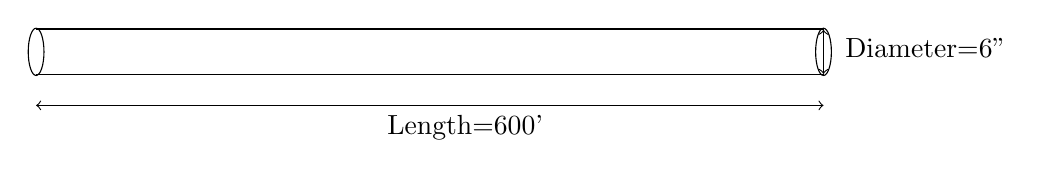
\begin{tikzpicture}
\draw (0,0) ellipse (0.1cm and 0.3cm);
\draw (10,0) ellipse (0.1cm and 0.3cm);
\draw [-] (0,-0.29) -- (10,-0.29);
\draw [-] (0,0.29) -- (10,0.29);
\draw [<->] (10,-0.28) -- (10,0.28) node [midway, below=-3mm] {\hspace{2.6cm}Diameter=6"};
\draw [<->] (0,-.68) -- (10,-.68)node [midway, below] {\hspace{0.9cm}Length=600'};
\end{tikzpicture}
% \end{center}
\vspace{0.3cm}
$Volume=\dfrac{\pi}{4}D^2*L=0.785*\Big(\dfrac{6}{12}\Big)^2*600\cancel{ft^3}*7.48\dfrac{gallons}{\cancel{ft^3}}=\boxed{881 \enspace gallons}$


\section{Flow and Velocity}\index{Flow and Velocity}
\begin{itemize}
\item Flow Rate - Q (volume/time) = velocity (distance or length traveled /time) * surface area
\item Velocity is the speed at which the water is flowing.  It is measured in units of length/time – ft./sec.
\item Velocity of water flowing through can be calculated by dividing the flow rate by area of the flow stream.\\
\vspace{0.5cm}
$$Velocity \enspace \dfrac{length}{time}= \dfrac{flow \enspace rate(\dfrac{volume \enspace or \enspace cubic \enspace length}{time})}{surface \enspace area \enspace in \enspace the \enspace direction \enspace of \enspace flow-square \enspace length}$$
\vspace{0.5cm}
\textbf{For a flow in a channel:}\\
\vspace{0.5cm}
\includegraphics[scale=0.5]{ChannelFlow3}\\

\textbf{For a flow in a pipe:}\\
\vspace{0.5cm}
\includegraphics[scale=0.65]{VelocityinPipe}\\
\vspace{0.5cm}
\end{itemize}

\textbf{Example 1:} If a chemical is added in a pipe where water is flowing at a velocity of 3.1 feet per second, how many minutes would it take for the chemical to reach a point 7 miles away?  \\

Note - we want the answer in minutes\\

$$\textrm{Min } = \dfrac{1}{3.1}\dfrac{sec}{ft}*\dfrac{5280ft}{mile}*7 miles*\dfrac{min}{60 sec} = \boxed{199 min}$$
\\

\textbf{Example 2:} Find the flow in cfs in a 6 -inch line, if the velocity is 2 feet per second.

\begin{enumerate}
\item Determine the cross-sectional area of the line in square feet. Start by converting the diameter of the pipe to inches.

The diameter is 6 inches: therefore, the radius is 3 inches. 3 inches is $3 / 12$ of a foot or $0.25$ feet.

\item Now find the area in square feet.
$$
\begin{aligned}
&A=\pi \times r^{2} \\
&A=\pi \times\left(0.25 \mathrm{ft}^{2}\right. \\
&A=\pi \times 0.0625 \mathrm{ft}^{2} \\
&A=0.196 \mathrm{ft}^{2}
\end{aligned}
$$
Or
$$
\begin{aligned}
&A=0.785 \times D^{2} \\
&A=0.785 \times 0.5^{2} \\
&A=0.785 \times .05 \times .05 \\
&A=0.196 \mathrm{ft}^{2}
\end{aligned}
$$

\item Now find the flow.

$\mathrm{Q}=\mathrm{V} \times \mathrm{A}$

$\mathrm{Q}=2 \mathrm{ft} / \mathrm{sec} \times 0.196 \mathrm{ft}^{2}$

$\mathrm{Q}=0.3927 \mathrm{cfs}$ or $0.4 \mathrm{cfs}$
\end{enumerate}


\section{Concentration}\index{Concentration}
\begin{itemize}
\item Concentration is typically expressed as mg/l which is the weight of the constituent (mg) in 1 liter of water.
\item As 1 liter of water weighs 1 million mg, a concentration of 1 mg/l implies 1 mg of constituent per 1 million mg of water or one part per million (ppm).   \texthl{Thus, mg/l and ppm are synonymous.}
\item Sometimes the constituent concentration is expressed in terms of percentage.\\
\vspace{6pt}
\textbf{Example:} 12.5\% chlorine concentration solution.\\
\vspace{0.2cm}
100\% would mean 1,000,000 mg/l or 1,000,000 ppm\\
\vspace{0.2cm}
$\implies$1\% would be $\dfrac{1,000,000}{100}\textrm{mg/l} = \textrm{10,000 mg/l or 10,000 ppm}$\\
\vspace{0.2cm}
$\implies$12.5\% chlorine concentration is 125,000 mg/l or 125,000 ppm.
\vspace{6pt}

$1\% \enspace concentration = 10,000 \enspace ppm \enspace or \enspace\dfrac{mg}{l}$\\
$0.1\% \enspace concentration = 1,000 \enspace ppm \enspace or \enspace \dfrac{mg}{l}$\\
$0.01\% \enspace concentration = 100 \enspace ppm \enspace or \enspace \dfrac{mg}{l}$\\
$10\% \enspace concentration = 100,000 \enspace ppm \enspace or \enspace \dfrac{mg}{l}$\\
$5\% \enspace concentration = 50,000 \enspace ppm \enspace or \enspace \dfrac{mg}{l}$\\
$12.5\% \enspace concentration = 125,000 \enspace ppm \enspace or \enspace \dfrac{mg}{l}$\\
\end{itemize}

\section{Density}\index{Density}
\begin{itemize}
\item Density is defined as the weight of a substance per a unit of its volume. For example, pounds per cubic foot or pounds per gallon.

\item Here are a few key facts about density:
\begin{itemize}

\item Density is measured in units of lb/ft3, lb/gal, or mg/L. Density of water = 62.4 lb/ft3 = 8.34 lb/gal.
\end{itemize}
\end{itemize}

\section{Specific Gravity}\index{Specific Gravity}
\begin{itemize}
\item Specific gravity is the ratio of the density of a substance (liquid or solid) to the density water.
\item It is the ratio of the weight of the substance of a certain volume to the weight of water of the same volume.

\item Any substance with a density greater than that of water will have a specific gravity greater than 1.0. Any substance with a density less than that of water will have a specific gravity less than 1.0. 

\item Specific gravity examples:
\begin{itemize}

\item Specific gravity of water = 1.0 
\item Specific gravity of concrete = 2.5 (depending on ingredients)
\item Specific gravity of alum (liquid @ 60°F) = 1.33 
\item Specific gravity of hydrogen peroxide (35\%) = 1.132
\end{itemize}

\item Specific gravity is used in two ways:
\begin{enumerate}
\item To calculate the total weight of a \% solution (either as a single gallon or a drum volume).\\
Total Weight = Drum Vol X SG X 8.34
\item To calculate the “active ingredient” weight of a single gallon or a drum.\\

Active Ingredient Weight within Drum = Drum Volume X SG X 8.34 X \% solution as a decimal. (i.e., Total Weight X \% solution as a decimal)\\

NOTE: Both ways start with solving for the total weight (Drum Vol X SG X 8.34). When solving for “active ingredient” weight, you have to then multiply by \% solution as a decimal.

\end{enumerate}
\end{itemize}

\textbf{Example:} What is the weight of 5 gallons of a 40\% ferric chloride solution given its specific gravity of 1.43?
$$(8.34 * 1.43) \enspace lbs/gal*5 \enspace gallons = \boxed{59.6 \enspace lbs}$$

The weight of active ferric chloride in the drum will be 59.6*0.4=23.84 lbs (as ferric chloride is 40\% strength)

\section{Detention Time}\index{Detention Time}
\begin{itemize}
\item \colorbox{lime}{Detention Time} - The actual or theoretical (calculated) time required for water to fill a tank at a given flow; pass through a tank at a given flow; or remain in a settling basin, flocculating basin, rapid-mix chamber, or storage tank.\\
$$Tank/clarifier \enspace detention \enspace time \enspace (hr) = 	\dfrac{ Tank/clarifier \enspace volume (cu.ft \enspace or \enspace gal)}{Influent \enspace flow \enspace (cu.ft \enspace or \enspace gal)/hr)}$$
Rectangular tank/clarifier volume = width * length * depth of water\\
Circular tank/clarifier volume = 0.785 * Diameter$^2$ * depth of water\\
Typically volume is calculated in cu. ft and influent flow is given in gallons.  Use 7.48 gal/ft$^3$ conversion factor to convert volume in cu. ft to gallons.\\
\end{itemize}


\section{Unit Conversions}\index{Unit Conversions}
\begin{itemize}
\item A conversion is a number that is used to multiply or divide into a measure in order to change the units of the original measure.

\begin{table}[h!]

\begin{center}
    \begin{tabular}{ | p{4cm} |p{8cm}|}
    \hline
    
\textbf{Measure} & \textbf{Units}\\
\hline   
Length  & inches, ft, miles\\
\hline 
Area  & ft$^2$, acres \\
\hline 
Volume & ft$^3$, gallons, acres-ft.\\
\hline 
Density & weight per volume, lbs/ft$^3$, lbs/gallon\\
\hline 
Flow & ft$^3$/min, MGD, acres-ft/day\\
\hline 

	

    \end{tabular}
 \caption{Common units in water calculations}	
    \end{center}

    \end{table}

\item In most instances, the conversion factor cannot be derived. It must be known. Therefore, tables such as the one below are used to find the common conversions.\\
\begin{tabular}{|l|l|}
\hline
Some Common Conversions & Weight \\
\hline
Linear Measurements & $1 \mathrm{ft}^{3}$ of water $=62.4 \mathrm{lbs}$ \\
\hline
1 inch $=2.54 \mathrm{~cm}$ & $1 \mathrm{gal}=8.34 \mathrm{lbs}$ \\
$1 \mathrm{foot}=30.5 \mathrm{~cm}$ & $1 \mathrm{lb}=453.6 \mathrm{grams}$ \\
$1 \mathrm{~meter}=100 \mathrm{~cm}=3.281 \mathrm{feet}=39.4$ inches 1 & $1 \mathrm{~kg}=1000 \mathrm{~g}=2.2 \mathrm{lbs}$ \\
acre $=43,560 \mathrm{ft}^{2}$ & $1 \%=10,000 \mathrm{mg} / \mathrm{L}$ \\
$1 \mathrm{yard}=3 \mathrm{feet}$ & $1 \mathrm{pound}=16 \mathrm{oz} \mathrm{dry} \mathrm{wt}$ \\
 & $1 \mathrm{ft}^{3}=62.4 \mathrm{lbs}$ \\
\hline
Volume & Pressure \\
\hline
$1 \mathrm{gal}=3.78$ liters & $1 \mathrm{ft}$ of head $=0.433 \mathrm{psi}$ \\
$1 \mathrm{ft}=7.48$ gal & $1 \mathrm{psi}=2.31 \mathrm{ft}$ of head \\
$1 \mathrm{~L}=1000 \mathrm{~mL}$ &  \\
$1 \mathrm{gal}=16 \mathrm{cups}$ &  \\
\hline
Flow &  \\
\hline
$1 \mathrm{cfs}=448 \mathrm{gpm}$ &  \\
$1 \mathrm{gpm}=1440 \mathrm{gpd}$ &  \\
\hline
\end{tabular}
\vspace{0.2cm}
\item Common conversions in water related calculations include the following:

\begin{itemize}
  \item gpm to cfs

  \item Million gallons to acre feet

  \item Cubic feet to acre feet

  \item Cubic feet of water to gallons


  \item gpm to MGD 

  \item psi to feet of head

\end{itemize}

\item Steps for unit conversion:\\
\begin{enumerate}[Step 1:]
\item \texthl{Make sure the original unit is for the same measurement as the converted (desired) unit.}  So if the original unit is for area, say in ft$^2$ the converted unit should be another area unit such as in$^2$ or acre but it cannot be gallons as gallon is a unit of volume.\\
Note:  Calculating the weight of a certain volume of water involves the use of density which is the mass per volume -  value in units including lbs/gallon or lbs/$ft^3$\\

\item Write down the conversion formula as:\\

$Quantity \enspace in \enspace converted \enspace unit = Quantity \enspace (\cancel{Original \enspace Unit}) *   Conversion  \enspace Factor \enspace  \dfrac{Conversion \enspace unit}{\cancel{Original \enspace unit}}$\\
\end{enumerate}

\item Note:  If you wish to convert cubic feet of water to pounds, you have to use its density which is the known mass per unit volume.\\
$\dfrac{8.34 \enspace lbs}{gallon}$ or $\dfrac{62.4 \enspace lbs}{ft^3}$\\
$mass \enspace of \enspace water = \cancel{Volume} *   Density  (\dfrac{mass}{\cancel{Volume}})$\\

\end{itemize}

Example Problems:\\
\begin{enumerate}
\item Convert 1000 $ft^3$ to cu. yards\\

$1000 \cancel{ft^3}*\dfrac{cu.yards}{27\cancel{ft^3}} = 37 cu.yards$

\item Convert 10 gallons/min to $ft^3$/hr\\
Note:  This involves use of two conversion factors - one for converting gallons to cubic feet and another for converting minute to gallons.\\ 
$\dfrac{10 \cancel{gallons}}{\cancel{min}}*  \dfrac{ft^3}{7.48 \cancel{gallons}}  * \dfrac{60 \cancel{min}}{hr}   = \dfrac{80.2ft^3}{hr}$


\item Convert 100,000 $ft^3$ to acre-ft.\\
$100,000 \cancel{ft^3} * \dfrac{acre-ft}{43,560 \cancel{ft^2-ft}} =  2.3 acre-ft$\\

\item Convert 8 $ft^3$ of water to pounds.\\
Here the conversion is from a volume ($ft^3$) to a weight (lbs).  It involves use of a standard correlation of the volume of water to its weight - its density. 

$Weight \enspace of \enspace water \enspace in \enspace lbs=8 \cancel{ft^3} *   62.4  (\dfrac{lbs}{\cancel{ft^3}}) = 499.2 \enspace lbs $\\

\end{enumerate}

\section{Pounds Formula}



Pounds formula is used for:
\begin{itemize}
\item Calculating the quantity in pounds of a particular wastewater constituent entering or leaving a wastewater treatment process
\item Calculating the pounds of chemicals to be added\\
\end{itemize}
So if the concentration of a particular constituent (in mg/liter) and the volume or flow of wastewater is given, one can calculate the amount of that constituent in pounds using the following – Pounds Formula:
$$lbs \enspace \textbf{or} \enspace \dfrac{lbs}{day}=concentration(\dfrac{mg}{l})*8.34*volume(MG) \enspace \textbf{or} \enspace flow(\dfrac{MG}{day}(MGD)$$

\begin{figure}[h!]
\begin{center}
\includegraphics[scale=0.5]{PoundsFormula}
\end{center}
\caption{Pounds formula "nomograph"}
\end{figure}
\vspace{0.3cm}
There are three variables – (lbs, concentration and volume) and one constant (8.34) in the pounds formula.  Knowing any of the two variables in the formula, one can calculate the third (unknown) variable by rearranging the equation.
\subsection{Example Problems}
% \hl{Example Problems}\\
\begin{enumerate}

\item If the influent wastewater flow is 5 MGD and the BOD concentration is 240 mg/l what is the daily BOD loading in lbs/day?\\
Solution:\\
$\dfrac{lbs \enspace BOD}{day}=5MGD*240mg/l*8.34=\boxed{\dfrac{10,000lbs}{day}}$\\

\item Calculate the lbs of solids in the primary sludge if the sludge flow is 7500 gallons and the solids concentration is 4.5\%.\\
Solution\\
Applying lbs formula:\\
$lbs \enspace solids = \dfrac{7500 \enspace MG}{1,000,000} * 4.5*10,000 *8.34 = \boxed{2,815 \enspace lbs \enspace solids}$\\
\textbf{Note:}\\  
1) 7500 gallons was converted to MG by dividing by 1,000,000\\
$7500 \enspace gallons * \dfrac{1 MG}{1,000,000 \enspace gallons}$\\
2) 4.5\% was converted to mg/l by multiplying by 10,000 as 1\%=10,000mg/l

\item An operator dissolves 1,200 lbs of a chemical in 12,000 gallons of water, what is the resultant concentration in mg/l, of the chemical solution?\\
Solution:\\
$Concentration \enspace \dfrac{mg}{l}=\dfrac{lbs}{Volume \enspace MG \enspace * \enspace 8.34}$\\
$Concentration \enspace \dfrac{mg}{l}=\dfrac{1,200}{0.012 \enspace * \enspace 8.34}=\boxed{\dfrac{11,990 \enspace mg}{l} \enspace or \enspace 1.2\% \enspace solution}$\\
\textbf{Note:}\\  
1) 12,000 gallons was converted to MG by dividing by 1,000,000\\
$12,000 \enspace gallons * \dfrac{1 MG}{1,000,000 \enspace gallons}$\\
\end{enumerate}
\section{Process Removal Efficiency Calculations}\index{Process Removal Efficiency Calculations}

\begin{itemize}
\item Process removal rate or removal efficiency is the percentage of the inlet concentration removed.  
\item It is used for quantifying the pollutant removal during wastewater treatment and is established based upon the amount of a particular wastewater constituent entering and leaving a treatment process.

\item $Process \enspace Removal \enspace Rate \enspace (\%) = \dfrac{Pollutant \enspace  In-Pollutant\enspace  Out}{Pollutant \enspace In}*100$\\

\item If 10 units of a pollutant are entering a process and 8 units of pollutant are leaving (process removes 2 units), then the process removal rate for that pollutant is (10-8)/10*100=20\%.  In this example the process is 20\% efficient in removing that particular pollutant.

\item The amount of pollutant can be measured in terms of concentration (mg/l) or in terms of mass loading (lbs).  The pounds formula is used for calculating the mass loadings.  
\end{itemize}
The above example is for calculating the removal efficiency using the inlet and outlet concentrations or mass loading.\\
The methods below can be used for calculating either the inlet or outlet pollutant concentrations, if the removal efficiency and the corresponding inlet or outlet concentrations are given. 


\hl{Case 1:  Calculating outlet conc. (X) given the inlet conc. and removal efficiency (RE\%):}

\tikzstyle{block} = [rectangle, draw, fill=red!40, 
    text width=6em, text centered, rounded corners, minimum height=3em]
\tikzstyle{arrow} = [draw, -latex']
\begin{figure}[!h]
\centering
\begin{tikzpicture}[node distance =1.5cm, auto]
    \draw ++(0,0) node [block] (Process) {Process};
   \node[node distance=1.9in] (dummy_in) [left of=Process] {In};
   \node[node distance=1.9in] (dummy_out) [right of=Process] {Out};
	\node (Removal) [below of=Process, yshift=-0in] {$\tiny{Removal \enspace Efficiency=RE\% \enspace (Given)}$};
    \path [arrow] (dummy_in)-- (Process)  node [above] {\hspace{-5.8cm}$A \enspace mg/l \enspace (Given) $} node [below] {\hspace{-5.8cm}$100 \enspace mg/l$};
    \path [arrow] (Process) -- (dummy_out)  node [above] {\hspace{-4cm}$X \enspace mg/l \enspace (Unknown)$} node [below] {\hspace{-3.9cm}($100-RE\%)\enspace mg/l$};
   \draw[arrow] (Process) -- (Removal);
\end{tikzpicture}
\end{figure}
Using the fact that if the inlet concentration was 100 mg/l, the outlet concentration would be 100 minus the removal efficiency.\\
Setup the equation as:  $\dfrac{Out}{In}: \enspace \dfrac{X \enspace mg/l}{A \enspace mg/l}=\dfrac{100-RE\%}{100}$\\
Calculate X using cross multiplication - if $\dfrac{A}{B}=\dfrac{C}{D} \implies A=B*\dfrac{C}{D}$:\\
$X \enspace mg/l=A \enspace mg/l*\dfrac{100-RE\%}{100}$\\

\hl{Case 2:  Calculating inlet conc. (X) given the outlet conc. and removal efficiency (RE\%):}

\begin{figure}[!h]
\centering
\begin{tikzpicture}[node distance =1.5cm, auto]
    \draw ++(0,0) node [block] (Process) {Process};
   \node[node distance=1.9in] (dummy_in) [left of=Process] {In};
   \node[node distance=1.9in] (dummy_out) [right of=Process] {Out};
	\node (Removal) [below of=Process, yshift=-0in] {$Removal \enspace Efficiency=RE\% \enspace (Given)$};
    \path [arrow] (dummy_in)-- (Process)  node [above] {\hspace{-5.8cm}$X \enspace mg/l \enspace (Unknown)$} node [below] {\hspace{-5.8cm}$100 \enspace mg/l$};
    \path [arrow] (Process) -- (dummy_out)  node [above] {\hspace{-4cm}$A \enspace mg/l \enspace (Given)$} node [below] {\hspace{-3.9cm}($100-RE\%)\enspace mg/l$};
   \draw[arrow] (Process) -- (Removal);
\end{tikzpicture}
\end{figure}
Using the fact that if the inlet concentration was 100 mg/l, the outlet concentration would be 100 minus the removal efficiency.\\
Setup the equation as:  $\dfrac{In}{Out}: \enspace \dfrac{X \enspace mg/l}{A \enspace mg/l}=\dfrac{100}{100-RE\%}$\\
\vspace{0.3cm}
Calculate X using cross multiplication - if $\dfrac{A}{B}=\dfrac{C}{D} \implies A=B*\dfrac{C}{D}$:\\
$X \enspace mg/l=A \enspace mg/l*\dfrac{100}{100-RE\%}$\\

\vspace{0.4cm}
\hl{Example Problems:}\\

\begin{enumerate}

\item What is the \% removal efficiency if the influent concentration is 10 mg/L and the effluent concentration is 2.5 mg/L?\\
$Removal \enspace Rate (\%) = \dfrac{In-Out}{In}*100 \implies \dfrac{10-2.5}{10}*100=\boxed{75\%}$



\item Calculate the outlet concentration if the inlet concentration is 80 mg/l and the process removal efficiency is 60\%\\
Solution:\\

\tikzstyle{block} = [rectangle, draw, fill=red!40, 
    text width=6em, text centered, rounded corners, minimum height=3em]
\tikzstyle{arrow} = [draw, -latex']
\begin{figure}[!h]
\centering
\begin{tikzpicture}[node distance =1.5cm, auto]
    \draw ++(0,0) node [block] (Process) {Process};
   \node[node distance=1.5in] (dummy_in) [left of=Process] {In};
   \node[node distance=1.5in] (dummy_out) [right of=Process] {Out};
	\node (Removal) [below of=Process, yshift=-0in] {$Removal \enspace Efficiency=60\%$};
    \path [arrow] (dummy_in)-- (Process)  node [above] {\hspace{-4.39cm}$80mg/l$} node [below] {\hspace{-4.39cm}$100mg/l$};
    \path [arrow] (Process) -- (dummy_out)  node [above] {\hspace{-3.cm}$Xmg/l$} node [below] {\hspace{-3cm}40mg/l};
   \draw[arrow] (Process) -- (Removal);
\end{tikzpicture}
%\caption[MFCC]{Diagrama en bloques del cálculo de las MFCC para un frame.}
%\label{MFCC}
\end{figure}

$\dfrac{Out}{In} \enspace:\enspace\dfrac{Actual \enspace Outlet (X)}{80}=\dfrac{100-60}{100}$\\
$\implies \dfrac{Actual \enspace Outlet (X)}{80} =0.4$\\
$\implies Actual \enspace  Outlet (X) = 0.4 * 80 = \boxed{32 mg/l}$\\


\item Calculate the inlet concentration if the outlet concentration is 80 mg/l and the process removal efficiency is 60\%\\

\tikzstyle{block} = [rectangle, draw, fill=red!40, 
    text width=6em, text centered, rounded corners, minimum height=3em]
\tikzstyle{arrow} = [draw, -latex']
\begin{figure}[!h]
\centering
\begin{tikzpicture}[node distance =1.5cm, auto]
    \draw ++(0,0) node [block] (Process) {Process};
   \node[node distance=1.5in] (dummy_in) [left of=Process] {In};
   \node[node distance=1.5in] (dummy_out) [right of=Process] {Out};
	\node (Removal) [below of=Process, yshift=-0in] {$Removal \enspace Efficiency=60\%$};
    \path [arrow] (dummy_in)-- (Process)  node [above] {\hspace{-4.39cm}$Xmg/l$} node [below] {\hspace{-4.39cm}$100mg/l$};
    \path [arrow] (Process) -- (dummy_out)  node [above] {\hspace{-3.cm}80mg/l} node [below] {\hspace{-3cm}40mg/l};
   \draw[arrow] (Process) -- (Removal);
\end{tikzpicture}
\end{figure}

$\dfrac{In}{Out} \enspace : \enspace \dfrac{Actual \enspace inlet \enspace  (X)}{80}=\dfrac{100}{100-60}\implies \dfrac{Actual \enspace inlet \enspace  (X)}{80}=2.5$\\    
Rearranging the equation:   $Actual \enspace inlet (X)=2.5*80 = \boxed{200 mg/l}$\\



\end{enumerate}

\section{Pounds Formula}\index{Pounds Formula}
\begin{itemize}
\item Pounds formula: 
$$lbs \enspace \textbf{or} \enspace \dfrac{lbs}{day}=Concentration\Big(\frac{mg}{l}\Big)*8.34*volume(MG) \enspace \textbf{or} \enspace Flow (MGD)$$\\
\item So if the concentration of a particular constituent (in mg/liter) and the volume or flow of wastewater is given, one can calculate the amount of that constituent or using this formula.\\
\texthl{Important notes:}\\
\begin{enumerate}
\item \texthl{The unit of the constituent loading rate will be in lbs per the unit of time the flow is expressed in.  So if the flow is in MG per day the calculated loading rate will be in lbs/day.  Likewise if the flow value used is in MG per minute, the calculated loading rate will be in lbs/min.}
\item \texthl{If volume is used, the calculated value will be the mass of the constituent in that volume.  If flow is used, the calculated value will be the mass of the constituent in that flow.}
\item \texthl{For the Pound Formula to work, the volume or flow needs to be expressed in MG.  Volume or flows in other units - gallons, $ft^3$ etc. needs to be converted to MG.}
\end{enumerate}

\item The formula assumes that all of the material found in water (TSS, BOD, MLSS, Chlorine, etc.) weighs the same as water, that is, $8.34$ pounds per gallon.
\item In the Pounds Formula, there are three variables – lbs, concentration and volume, and one constant - 8.34.  Knowing any of the two variables in the formula, one can calculate the third (unknown) variable by rearranging the equation.\\
\begin{figure}[h]
\begin{tikzpicture}
    \newcommand{\R}{3}

\path[help lines,step=.2] (0,0) grid (16,6);
\path[help lines,line width=.6pt,step=1] (0,0) grid (16,6);
%\foreach \x in {0,1,2,3,4,5,6,7,8,9,10,11,12,13,14,15,16}
%\node[anchor=north] at (\x,0) {\x};
%\foreach \y in {0,1,2,3,4,5,6}
%\node[anchor=east] at (0,\y) {\y};
%-------------CIRCLE-----------------------------------
\draw[black,fill=gray!10] (8,3) circle (\R);
\draw[black, very thick, rotate=0](5,3) -- (11,3);
\draw (8,4.5) node[text width=3cm,align=center]
  {\scriptsize{lbs or lbs/day}};
\draw (6.4,2) node[text width=3cm,align=center]
  {\scriptsize{Concentration\\mg/l}};
\draw (9.7,2) node[text width=3cm,align=center]
  {\scriptsize{Volume(MG)\\Flow(MGD)}};
  \draw (8,1)node[text width=3cm,align=center]
  {\scriptsize{8.34}};
\draw[black, very thick, rotate=0](6.4,0.5) -- (8,3);
\draw[black, very thick, rotate=0](9.6,0.5) -- (8,3);
  \node [circle split,draw,double,fill=red!20] at (4,3)
  {
    % No \nodepart has been used, yet. So, the following is put in the
    % ``text'' node part by default.
    $\div$
    \nodepart{lower} % Ok, end ``text'' part, start ``output'' part
    $=$
  };
  
    \node [circle split,draw,double,fill=red!20] at (5.8,-0.2)
  {
    % No \nodepart has been used, yet. So, the following is put in the
    % ``text'' node part by default.
    \scriptsize{$X$}
    \nodepart{lower} % Ok, end ``text'' part, start ``output'' part
    \tiny{$Multiply$}
  };
  
    \node [circle split,draw,double,fill=red!20] at (10,-0.2)
  {
    % No \nodepart has been used, yet. So, the following is put in the
    % ``text'' node part by default.
    \scriptsize{$X$}
    \nodepart{lower} % Ok, end ``text'' part, start ``output'' part
    \tiny{$Multiply$}
  };
\end{tikzpicture}
\caption{Davidson Pie}
\end{figure}
\vspace{0.2cm}
\item Davidson Pie provides a pictorial reference for calculating any unknown variable.  If for example, if Concentration is unknown, it can be calculated as follows: \\$$Concentration\Big(\frac{mg}{l}\Big)=\dfrac{lbs \enspace \textbf{or} \enspace \dfrac{lbs}{day}}{8.34*Volume(MG) \enspace \textbf{or} \enspace Flow (MGD)}$$\\
\vspace{0.2cm}
\item Likewise, if Volume (or Flow) is the unknown variable. it can be calculated as:  \\$$Volume (MG) \enspace or \enspace Flow(MGD)=\dfrac{lbs \enspace \textbf{or} \enspace \dfrac{lbs}{day}}{Concentration\Big(\dfrac{mg}{l}\Big)* \enspace 8.34  }$$
\vspace{0.2cm}
\item Pounds formula is used for:
\begin{itemize}
\item Calculating the quantity in pounds of a particular wastewater constituent entering or leaving a wastewater treatment process
\item Calculating the pounds of chemicals to be added\\
\end{itemize}
\end{itemize}


\textbf{Example 1:} If a 5 MGD flow is to be dosed with 25 mg/l of a certain chemical, calculate the lbs/day that chemical required.\\

Solution\\

Applying lbs formula:\\
$\dfrac{lbs}{day}=5 MGD *250\dfrac{mg}{l}*8.34 = \boxed{1,042\dfrac{lbs}{day}}$
\\
\vspace{6pt}
\textbf{Example 2:} Calculate the lbs of chemical in 7,500 gallons of 4.5\% active solution of that chemical.\\
Solution\\
Applying lbs formula:\\
$lbs chemical = \dfrac{7500}{1,000,000}MG * 4.5*10,000 *8.34 = \boxed{2,815 \enspace lbs \enspace chemical}$\\
\textbf{Note:}\\  
1) 7500 gallons was converted to MG by dividing by 1,000,000\\
$7500 \enspace gallons * \dfrac{1 MG}{1,000,000 \enspace gallon}$\\
2) 4.5\% was converted to mg/l by multiplying by 10,000 as 1\%=10,000mg/l


\section{Chemicals Related Math Problems}\index{Chemicals Related Math Problems}
\subsection{Chemical Dosing}\index{Chemical Dosing}

\begin{itemize}
\item Use lbs formula to calculate the lbs of chemicals required\\
\item Using the calculated lbs chemical required value, calculate the amount of that chemical at the concentration available
\end{itemize}

So for example, if asked how much many gallons per day of bleach solution (SG 1.2)containing 12.5\% available chlorine is required to disinfect a 10 MGD flow of water given the required chlorine dosage of 7 mg/l.\\
\begin{enumerate}
\item calculate the lbs of chlorine required using the lbs formula:\\
\vspace{0.5cm}
=$10 MGD \enspace * \enspace 7 \dfrac{mg}{l} \enspace * \enspace 8.34\enspace=\enspace 583.8 \enspace lbs \enspace chlorine \enspace per \enspace day$\\
\vspace{0.5cm}
\item calculate the gallons of bleach which will provide the 583.8 lbs chlorine\\
\vspace{0.5cm}
Applying the lbs formula - note that 8.34 * SG will give the actual lbs/gal of bleach.  If SG is not provided, use only 8.34 lbs per gallon:\\
\vspace{0.5cm}
$583.8 \dfrac{lbs \enspace bleach}{day}\enspace=\enspace x \dfrac{gal}{day} \enspace * \enspace 8.34 * 1.2 \dfrac{lbs \enspace bleach}{gal} \enspace * \enspace 0.0125 \dfrac{lbs \enspace chlorine}{lb \enspace bleach} \enspace $\\
\vspace{0.5cm}
$ \implies x \dfrac{gal}{day}\enspace = \enspace \dfrac{583.8}{8.34*1.2*0.125} \enspace = \boxed{467 \dfrac{gal}{day}}$
\end{enumerate}
\vspace{0.3cm}
\textbf{The above problem can be solved directly using the formula below given in the SWRCB Water Treatment Exam Formula Sheet.}\\
\vspace{0.3cm}
 $\textrm{GPD}=\dfrac{\textrm{(MGD)}*\textrm{(ppm or mg/l)}*8.34 \enspace \textrm{lbs/gal}}{\textrm{\% \enspace purity}*\textrm{Chemical \enspace Wt. (lbs/gal)}}$ 
 \vspace{0.3cm}
 $\textrm{GPD}=\dfrac{10*7*8.34}{0.125*(1.2*8.34)}=\boxed{467 \dfrac{\textrm{gal}}{\textrm{day}}}$ 
 
\subsection{Chemical Dilution} \index{Chemical Dilution}
\begin{itemize}
\item Chemicals obtained in bulk are typically delivered in higher concentrations to reduce transportation costs and need dilution to ensure proper mixing and dosage control.

\item Thus, for dilution calculations, if:\\
\vspace{0.2cm}
C$_1$ and V$_1$ is the concentration and volume respectively of the concentrated chemical used for the dilution, and\\
\vspace{0.2cm}
C$_2$ and V$_2$ is the concentration and volume of the product after dilution with water\\
\vspace{0.2cm}
As, the mass of the target chemical in the volume of the concentrated product used for dilution will remain the same in the final diluted product:\\
\vspace{0.3cm}
\textbf{C$_1$ * V$_1$ =  C$_2$ * V$_2$.}\\

\item Thus, knowing C$_1$, C$_2$ and V$_2$, we can calculate V$_1$ as: $$V_1 = \frac{C_2 * V_2}{C_1}$$
\end{itemize}

\textbf{Example Problem:}\\
\vspace{0.2cm}
How much initial volume of a 4\% polymer solution is needed to make 3500 gallons of polymer at 0.25\% concentration.\\
\vspace{0.2cm}
Solution:\\
\vspace{0.2cm}
$$V_{4\%} = \frac{C_{.25\%} * V_{.25\%}}{C_{4\%}} = \frac{0.25 \enspace * \enspace 3500}{4}= 219 gal $$ 
\vspace{0.2cm}
So take 219 gallons of the 4\% polymer and dilute to 3500 gallons to give a 0.25\% polymer solution.


\section{Preliminary Treatment} \index{Preliminary Treatment}

\section{Preliminary Treatment Math Problems}\index{Preliminary Treatment Math Problems}

Preliminary Treatment math problems relate to the following:

\subsection{Channel Velocity and Flow Rate}\index{Channel Velocity and Flow Rate}
Flow Rate - Q (volume/time) = velocity (distance or length traveled /time) * surface area\\
Velocity is the speed at which the water is flowing.  It is measured in units of length/time – ft./sec.\\
Velocity of water flowing through can be calculated by dividing the flow rate by area of the flow stream.\\
\vspace{0.5cm}
$Velocity \enspace \dfrac{length}{time}= \dfrac{flow \enspace rate(\dfrac{volume \enspace or \enspace cubic \enspace length}{time})}{surface \enspace area \enspace in \enspace the \enspace direction \enspace of \enspace flow-square \enspace length}$\\
\vspace{0.5cm}
\textbf{For a flow in a channel:}\\
\vspace{0.5cm}
\hl{Example Problems:}\\
\begin{enumerate}[1.]
\item Calculate the velocity of a 14 MGD flow in a 6 ft wide channel with a water depth of two feet.\\
\begin{center}
\includegraphics[scale=0.5]{ChannelFlow3}
\end{center}
$Flow (Q) = Velocity (V) * Area (A)$\\
$\implies 14 \dfrac{MG}{day}* \dfrac{10^6 gal}{MG} * \dfrac{ft^3}{7.48 gal}*\dfrac{day}{24*60*60} = V \dfrac{ft}{sec}* 6 ft * 2 ft \implies 21.7 \dfrac{ft^3}{sec}= 12V\dfrac{ft^3}{sec}$\\
$\implies V \dfrac{ft}{sec}= \dfrac{21.7}{12}= \boxed{1.8\dfrac{ft}{sec}}$\\

\item Calculate the flow, in gpd, that would pass through a grit chamber 2 feet wide, at a depth of 6 inches, with a velocity of 1 ft /sec\\
Solution:\\
\includegraphics[scale=0.5]{ChannelFlow3}\\
$Q=V*A$\\
$Q=1\dfrac{ft}{s}*(2*0.5)ft^2=1\dfrac{ft^3}{s}$\\
$Q=1\dfrac{\cancel{ft^3}}{\cancel{s}}*\dfrac{(1440*60)\cancel{s}}{day}*7.48\dfrac{gal}{\cancel{ft^3}}=\boxed{646,272\dfrac{gal}{day}}$
\vspace{0.5cm}
\item A wastewater channel is 3.25 feet wide and is conveying a wastewater flow of 3.5 MGD. The wastewater flow is 8 inches deep. Calculate the velocity of this flow.\\
Solution:\\
\includegraphics[scale=0.5]{ChannelFlow3}\\
$Q=V*A \implies V=\dfrac{Q}{A}$\\
$\implies V\dfrac{ft}{s}=\dfrac{3.5\dfrac{\cancel{MG}}{\cancel{day}}*\dfrac{1000000\cancel{gal}}{\cancel{MG}}*\dfrac{ft^{\cancel{3}}}{7.48\cancel{gal}}*\dfrac{\cancel{day}}{(1440*60)s}}{(3.25*0.75)\cancel{ft^2}}=\boxed{2.2\dfrac{ft}{s}}$
\vspace{0.5cm}
\item A plastic float is dropped into a wastewater channel and is found to travel 10 feet in 4.2 seconds. The channel is 2.4 feet wide and is flowing 1.8 feet deep. Calculate the flow rate of this wastewater in cubic feet per second.\\
Solution:\\
$Q=V*A$\\
$\implies Q\Big(\dfrac{ft^3}{s}\Big)=\dfrac{10ft}{4.2s}*(2.4*1.8)ft^2=\boxed{10.3\dfrac{ft^3}{s}}$
\end{enumerate}

\subsection{Grit Removal Rates}\index{Grit Removal Rates}
\emph{Typical grit removal ranges from 0.5 to 30 ft$^3$/MG}\\
\vspace{0.3cm}
\hl{Example Problems:}\\
\begin{enumerate}[1.]
\item At a wastewater treatment plant which receives a flow rate of 650,000 gallons per day, a total of 50 cubic feet of grit was removed for the month. Calculate the rate of grit removal assuming 30 days in a month.\\
Solution:\\
$Grit Removal\dfrac{ft^3}{MG}=50\dfrac{ft^3}{ \cancel{month}}*\dfrac{\cancel{month}}{30\cancel{days}}*\dfrac{\cancel{day}}{650,000\cancel{gal}}*1,000,000\dfrac{\cancel{gal}}{MG}=\boxed{2.6\dfrac{ft^3}{MG}}$
\end{enumerate}

\section{Primary Treatment} \index{Primary Treatment}
\subsection{Hydraulic or Surface Loading Rate}\index{Hydraulic or Surface Loading Rate}

The hydraulic or surface loading rate measures how rapidly wastewater moves through the primary clarifier.  It is measured in terms of the number of gallons flowing each day through one square foot surface area of the clarifier. 
$$Clarifier \enspace hydraulic \enspace loading \enspace 	\Big(\dfrac{gpd}{ft^2}\Big) =\dfrac{Clarifier \enspace influent 	\enspace flow (gpd)}{Clarifier \enspace surface \enspace area 	(ft^2)}$$ 
		Rectangular clarifier surface area  = width * length\\
		Circular clarifier surface area  = 0.785 * Diameter$^2 $\\
\subsection{Detention Time}\index{Detention Time}

Detention time is the length of time that wastewater stays in the settling tank is called the detention time.  It is also the time it takes for a unit volume of wastewater to pass entirely through a primary clarifier\\
$$Clarifier \enspace detention \enspace time \enspace (hr) = 	\dfrac{ Clarifier \enspace volume (cu.ft \enspace or \enspace gal)}{Influent \enspace flow \enspace (cu.ft \enspace or \enspace gal)/hr)}$$
Rectangular clarifier volume = width * length * depth of water\\
Circular clarifier volume = 0.785 * Diameter$^2$ * depth of water\\
Typically volume is calculated in cu. ft and influent flow is given in gallons.  Use 7.48 gal/ft$^3$ conversion factor to convert volume in cu. ft to gallons.\\

\subsection{Weir Overflow Rate}\index{Weir Overflow Rate}
The weirs at the end of the primary clarifier allow for the even distribution of the the outlet flow across the entire length of the weir.  An adequate length of weir is needed to ensure smooth and even flow of wastewater over the weirs.  Weir overflow rate measures the number of gallons of wastewater per day flowing over one foot of weir. 

		$$Weir \enspace over \enspace flow \enspace rate \Big(\dfrac{gpd}{ft}\Big) =\Big(\dfrac{Clarifier \enspace influent \enspace  flow (gpd)}{Total \enspace effluent 					\enspace weir \enspace length \enspace (ft)}\Big)$$
		Circular clarifier weir length = 3.14 * Diameter\\

\hl{Example problem for (a), (b) and (c) above:}\\
		\vspace{0.2cm}
A circular clarifier receives a flow of 11 MGD.  If the clarifier is 90 ft. in diameter and is 12 ft. deep, what is: a) the hydraulic/surface loading rate, b) clarifier detention time in hours, and c) weir overflow rate?\\
		\vspace{0.2cm}
a) Hydraulic/surface loading rate:\\
$Clarifier \enspace hydraulic \enspace loading \enspace 	\Big(\dfrac{gpd}{ft^2}\Big) ==\dfrac{\dfrac{11\cancel{MG}}{{day}}*\dfrac{10^6gal}{\cancel{MG}}}{0.785*90^2 ft^2}=\boxed{1,730gpd/ft^2}$\\
		\vspace{0.5cm}
b) Clarifier detention time:\\
$Clarifier \enspace detention \enspace time \enspace (hr) = 	\dfrac{ Clarifier \enspace volume (cu.ft \enspace or \enspace gal)}{Influent \enspace flow \enspace (cu.ft \enspace or \enspace gal)/hr)}$\\
		\vspace{0.2cm}
$Clarifier \enspace detention \enspace time \enspace (hr) = 	\dfrac{(0.785*90^2*12)\cancel{ft^3}}{\dfrac{11\cancel{MG}}{\cancel{day}}*\dfrac{10^6\cancel{gal}}{\cancel{MG}}*\dfrac{\cancel{ft^3}}{7.48\cancel{gal}}*\dfrac{\cancel{day}}{24hrs}}=\boxed{1.2hrs}$\\
		\vspace{0.5cm}
c) Weir overflow rate:\\
		\vspace{0.2cm} 
$Weir \enspace overflow \enspace rate \Big(\dfrac{gpd}{ft}\Big) =\dfrac{\dfrac{11\cancel{MG}}{{day}}*\dfrac{10^6gal}{\cancel{MG}}}{3.14*90 ft}=\boxed{38,924gpd/ft}$\\

\subsection{Removal Efficiency}\index{Removal Efficiency}		
Primary sedimentation removes suspended wastewater solids which includes BOD.  The efficiency of the primary is established as the percentage of the amount of parameter removed.  The parameter may quantified as mass (lbs) or as concentration (mg/l).

$$Removal \enspace efficiency (\%) = \dfrac{Parameter  \enspace In - Parameter  \enspace Out}{Parameter \enspace In} * 100$$

For TSS removal:\\
$$TSS \enspace Removal \enspace efficiency (\%) = \dfrac{TSS  _{In} \enspace(mg/l)  - TSS_{Out} \enspace(mg/l)  }{TSS _{In} \enspace(mg/l)  } * 100$$

For BOD removal:\\
$$BOD \enspace Removal \enspace efficiency (\%) = \dfrac{BOD_{In} \enspace(mg/l)  - BOD_{Out} \enspace(mg/l)  }{BOD _{In} \enspace(mg/l)  } * 100$$
\subsection{Solids Removal}\index{Solids Removal}	

\hl{\textbf{Type 1 Problems:}  These involve calculating lbs of solids removed given any two of the following TSS parameters - inlet concentration, outlet concentration and removal efficiency.}\\
a. If the inlet and outlet concentrations are given, calculate the mg/l of TSS removed using: 
$$TSS_{removed} = TSS_{in}(mg/l) - TSS_{out} (mg/l) $$
Then knowing the flow, use the lbs formula to calculate the lbs solids removed.

b. If either inlet or outlet concentration is given along with the clarifier removal efficiency, using the removal efficiency calculate the unknown outlet concentration (if only the inlet is given) or the inlet concentration (if only the outlet is given)\\
i) If inlet and removal efficiency is given, calculate the outlet by subtracting the product of inlet and removal efficiency from the inlet.
$$TSS_{out}=TSS_{in} - (TSS_{in}*\%Removal)$$
Example if the removal efficiency is 60\% and the inlet concentration is 300mg/l: $$TSS_{out}=300 - 300*0.6=120mg/l$$
ii) If outlet and removal efficiency is given, calculate the inlet concentration by dividing the outlet by (1-removal efficiency).\\
$$TSS_{in}=\dfrac{TSS_{out}}{1-\%Removal}$$
Example if the removal efficiency is 60\% and the outlet concentration is 120mg/l: $$TSS_{in}=\dfrac{120}{1-0.6}=300mg/l$$ 

Note:  You may derive the above formulas by algebraically manipulating: $\%Removal=\dfrac{TSS_{in} -TSS_{out}}{TSS_{in}}$\\
\hl{Example Problem:}\\
How many lbs of solids are removed daily by a primary clarifier treating a 6 MGD flow if the average influent TSS concentration is 300 mg/l and the clarifier TSS removal efficiency is 67\%.\\
$TSS_{out}=(300mg/l - 300*0.67)=99mg/l$\\
$lbs \enspace solids \enspace  removed = (300-99)mg/l*8.34*6MGD=\boxed{10,058 \enspace lbs \enspace solids \enspace removed \enspace per \enspace day}$\\
\vspace{0.5cm}
\hl{\textbf{Type 2 Problems:}  These involve calculating the amount of sludge pumping given the solids removed.  The solids removed from the primary clarifier is sludge with a typical solids concentration of about 3\% to 5\%.}\\
Given the amount of total solids removed and given the sludge concentration, the volume of sludge pumping can be calculated as follows:  $$\dfrac{ft^3\enspace sludge\enspace pumped}{ day}= \dfrac{lbs \enspace solids \enspace (removed)}{day} * \dfrac{1 \enspace lb \enspace sludge}{(\%)\enspace lbs \enspace solids}*\dfrac{gal \enspace sludge}{8.34lb \enspace sludge}*\dfrac{ft^3 \enspace sludge}{7.48 \enspace gal} $$
So for the solids removed in the above example, if the primary sludge has 5\% solids, the required sludge pumping can be calculated as:
$$\dfrac{ft^3\enspace sludge}{day}= \dfrac{10,058 \enspace \cancel{lbs \enspace solids}}{day} * \dfrac{1 \enspace \cancel{lb \enspace sludge}}{0.05\enspace \cancel{lbs \enspace solids}}*\dfrac{\cancel{gal \enspace sludge}}{8.34\cancel{lb \enspace sludge}}*\dfrac{ft^3 \enspace sludge}{7.48 \enspace \cancel{gal}}=\boxed{3,224\dfrac{ft^3 \enspace sludge}{day}} $$


\section{Trickling Filter Calculations}\index{Trickling Filter Calculations}

Trickling filter problems involve calculation of the following:

\subsection{Hydraulic or surface loading}\index{Hydraulic or surface loading}

\begin{itemize}
\item Hydraulic or surface loading is expressed as gpd/$ft^2$
\item \hl{The gpd is the total flow (Q$_T$)to the filter - primary influent flow + recirculated flow(Q$_T$= Q$_I$ + Q$_R$)}\\
\end{itemize}
			\hl{Example Problem:}\\
The total influent flow (including recirculation) to a trickling filter is 1.89 MGD. If the trickling filter is 80 ft in diameter, what is the hydraulic loading in gpd/sq ft on the trickling filter?\\
\vspace{0.2cm}
Solution:\\
\vspace{0.2cm}
$Hydraulic \enspace loading \enspace \dfrac{gpd}{ft^2}=\dfrac{(1.89*10^6)gpd}{(0.785*80^2)ft^2} =\boxed{376\dfrac{gpd}{ft^2}}$
			
			
\subsection{BOD and TSS Removal}\index{BOD and TSS Removal}
BOD and  removal is based upon the TF influent and effluent concentrations.\\
\vspace{0.2cm}
$\% Removal=\dfrac{In_{conc}-Out_{conc}}{In_{conc}}*100$\\
			\hl{Example Problem:}\\
The suspended solids concentration entering a trickling filter is 236 mg/l. If the suspended solids concentration of the trickling filter effluent is 33 mg/l, what is the suspended solids removal efficiency of the trickling filter?\\
\vspace{0.2cm}
Solution:\\
\vspace{0.2cm}
$\% Removal=\dfrac{236 mg/l-33 mg/l}{236 mg/l}*100=\boxed{86\%}$

\subsection{Organic Loading}\index{Organic Loading}

			\begin{itemize}
\item Organic loading to a trickling filter is typically expressed as lbs BOD/(day-1000 cu ft).  \item The lbs/day BOD value is the BOD loading from the primary effluent.
\item The 1000 ct. ft is the volume of the media.  
\item The media volume is calculated by multiplying the TF surface area by the media height.  
\item As the dimensions are typically given in ft., calculate the volume in $ft^3$ and then divide the calculated volume by 1000 to give the volume in units of 1000$ft^3$\\
\end{itemize}
\hl{Example Problem:}\\
A trickling filter, 70 ft in diameter with a media depth of 6 ft, receives a flow of 0.78 MGD. If the BOD concentration of the primary effluent is 167 mg/L, what is the organic loading on the trickling filter in lbs BOD/day/1000 cu ft?\\
Solution:  $Organic \enspace loading:\dfrac{lbs \enspace BOD}{day-1000ft^3}=\dfrac{lbs \enspace BOD \enspace feed \enspace to \enspace TF \enspace per \enspace day}{volume \enspace in \enspace 1000ft^3}$\\
$=\dfrac{\dfrac{(0.78*167*8.34)lbs \enspace BOD}{day}}{(0.785*70^2*6)ft^3*\dfrac{1000ft^3}{1000ft^3}}=\boxed{\dfrac{47 lbs \enspace BOD}{day-1000 ft^3}}$

\subsection{Recirculation Ratio}\index{Recirculation Ratio}


$Recirculation \enspace Ratio (R_R)=\dfrac{Recirculated \enspace Flow (Q_R)}{Influent  \enspace  Flow (Q_I)}$\\
\vspace{0.5cm}
$Recirculation \enspace Ratio (R_R)=\dfrac{Total \enspace Flow (Q_T) - Influent \enspace Flow (Q_I)}{Influent  \enspace  Flow (Q_I)}$\\
\vspace{0.5cm}
$Total \enspace Flow (Q_T) = Influent \enspace Flow (Q_I)*(Recirculation \enspace Ratio(R_R) +1)$
Make sure $Q_R$, $Q_T$ and $Q_I$ units are the same in a given problem

\hl{Example Problems:}\\
\begin{enumerate}
\item The influent to the trickling filter is 1.61 MGD. If the recirculated flow is 2.27 MGD, what is the recirculation ratio?\\
\vspace{0.2cm}
Solution:  $R_R=\dfrac{Q_R}{Q_I}=\dfrac{2.27}{1.61}=\boxed{1.4}$\\
\vspace{0.2cm}
\item A trickling filter has a total flow of 32 MGD.  If the recirculation ratio is 0.8, what is the primary effluent flow to the TF?\\
\vspace{0.2cm}
Solution:\\
\vspace{0.2cm}
$Total \enspace Flow (Q_T) = Influent \enspace Flow (Q_I)*(Recirculation \enspace Ratio(R_R) +1)$\\
$\implies 32 MGD=Q_I*(0.8+1)\implies Q_I=\dfrac{32}{1.8}=\boxed{17.8 MGD}$
\end{enumerate}




\section{Stabilization Pond Calculations} \index{Stabilization Pond Calculations}
\subsection{Pond Area}\index{Pond Area}

Formula: \hl{$Pond \enspace Area=Width * Length$}\\
\vspace{0.2cm}
also,     \hl{$Pond \enspace Area=\dfrac{Pond \enspace Volume}{Pond \enspace Depth}$}\\
\vspace{0.2cm}
\hl{Example Problem:}\\
A pond is 260 ft. long and 80 ft. wide. What is the area of this pond in acres?\\ 
\vspace{0.2cm}
Solution:\\
\vspace{0.2cm}
$(260*80)ft^2*\dfrac{acre}{43,560ft^2}=\boxed{0.48acre}$

\subsection{Solids Loading Rate}\index{Solids Loading Rate}


Formula: \hl{$Pond \enspace TSS \enspace loading \enspace rate =  \dfrac{lbs \enspace TSS}{day}$}  \\
\vspace{0.3cm}
\hl{Example Problem:}\\
\vspace{0.3cm}

The influent flow to a pond is 10,000 gallons/hour with a suspended solids concentration of 142mg/L in the raw wastewater.  How many lbs of suspended solids are sent to the pond daily?
\\
Solution:\\
\vspace{0.3cm}
$\dfrac{lbs \enspace TSS}{day}=10,000\dfrac{gal}{hr}*\dfrac{24hrs}{day}*\dfrac{MG}{1,000,000gal}*142\dfrac{mg}{l}*8.34=\boxed{284\dfrac{lbs \enspace TSS}{day}}$

\vspace{0.3cm}

\subsection{Organic Loading Rate}\index{Organic Loading Rate}

\vspace{0.3cm}
Formula: \hl{$Pond \enspace organic \enspace loading \enspace rate =  \dfrac{lbs \enspace BOD/day}{Area (acre)}$}  \\
\vspace{0.3cm}
\hl{Example Problem:}\\
\vspace{0.3cm}
The flow to a pond is 7.2MGD. If the pond diameter is 350 ft and the BOD in the pond influent is 170mg/L, what is the organic loading to this pond in lbs BOD/day/acre?
\\
Solution:\\
\vspace{0.3cm}
$Organic \enspace loading=\dfrac{lbs \enspace BOD \enspace per \enspace day}{area \enspace (acres)}=\dfrac{(7.2MGD \enspace * \enspace 170mg/l \enspace * \enspace 8.34)}{0.785*350^2ft^2}*\dfrac{43,560ft^2}{acre}=\boxed{\dfrac{4,624lbs \enspace BOD}{day-acre}}$

\vspace{0.3cm}

\subsection{Detention time}\index{Detention time}
\vspace{0.3cm}
Formula: \hl{$Pond \enspace detention \enspace time=\dfrac{Volume}{Flow}$}\\ 
\vspace{0.3cm}
\hl{Example Problem:}\\
A 40 acre wastewater treatment pond receives a flow of 0.6 MGD. If the pond is operated at a depth of 4ft. What is the detention time of this pond?\\
Solution:\\
$Pond \enspace detention \enspace time=\dfrac{Volume}{Flow}=\dfrac{(40*4)acre-ft}{0.6*10^6\dfrac{gal}{day}*\dfrac{ft^3}{7.48gal}*\dfrac{acre-ft}{43,560ft^3}}=\boxed{87 \enspace days}$\\
\vspace{0.3cm}


\subsection{Hydraulic Loading Rate}\index{Hydraulic Loading Rate}
Formula:\hl{$Pond \enspace hydraulic \enspace loading \enspace rate \enspace \Bigg[\dfrac{in}{day}\Bigg]=\dfrac{Flow}{Area}$}\\
also, \hl{$Pond \enspace hydraulic \enspace loading \enspace rate \Bigg[\dfrac{in}{day}\Bigg]=\dfrac{Pond \enspace depth \enspace (in)}{Pond \enspace detention  \enspace time \enspace \dfrac{Volume}{Flow}}$ }\\
The second formula above is because:\\
\vspace{0.3cm}
$Hydraulic \enspace Loading \enspace (HL)=\dfrac{Flow}{Area}$\\
\vspace{0.3cm}
$Detention \enspace time \enspace (DT)=\dfrac{Vol}{Flow} \implies Flow=\dfrac{Vol}{DT} $\\
\vspace{0.3cm}
Substituting for flow in  the HL formula above:\\
\vspace{0.3cm}
$HL=\dfrac{\dfrac{Vol}{DT}}{Area}\enspace or \enspace \dfrac{Vol}{Area*DT} \enspace \implies \boxed{HL=\dfrac{Pond \enspace Depth}{DT}} \enspace as \enspace \dfrac{Vol}{Area}=Pond \enspace Depth$\\
\vspace{0.3cm}
\textbf{Example Problems:}\\
\begin{enumerate}

\item Find hydraulic loading in inches/day for a pond given the following:
\begin{itemize}
\item Pond depth = 12ft.
\item Pond volume = 1,400,000ft3
\item Pond flow = 1,000,000gal/day
\end{itemize}
Solution:\\
$Pond \enspace hydraulic \enspace loading \enspace rate \enspace \Bigg[\dfrac{in}{day}\Bigg]=\dfrac{Flow}{Area}$\\
$ \implies\dfrac{1,000,000\dfrac{gal}{day}*\dfrac{ft^3 }{7.48gal}}{\dfrac{1,400,000ft^3}{12ft}}*12\dfrac{in}{ft}=\boxed{13.8\dfrac{in}{day}}$\\
\vspace{0.3cm}
\hl{Note:  The area of the pond was found by dividing the volume (1,000,000$ft^3$) by the pond depth (12ft)}
\vspace{0.3cm}

\item Find pond hydraulic loading in inches/day when the depth of the pond is 6 ft. and the detention time is 30 days.\\
Solution:\\



$Pond \enspace hydraulic \enspace loading \enspace rate=\dfrac{Pond \enspace depth \enspace (in)}{Pond \enspace detention  \enspace time \enspace \dfrac{Volume}{Flow}}$\\
$\implies \dfrac{6*12 \enspace inches}{30 \enspace days}=\boxed{\dfrac{2.4in}{day}}$
\end{enumerate}


\section{Activated Sludge Calculations} \index{Activated Sludge Calculations}
\subsection{Mean Cell Residence Time}\index{Mean Cell Residence Time}


The MCRT is calculated as:\\  
\vspace{0.2cm}
$MCRT(days) = $\\
$\dfrac{Total \enspace MLSS \enspace lbs \enspace in \enspace the \enspace aeration \enspace system \enspace (aeration \enspace tank \enspace + \enspace clarifier)}{Total \enspace amount \enspace in \enspace lbs/day \enspace of \enspace suspended \enspace solids \enspace leaving  \enspace the \enspace system \enspace(Effluent\enspace SS+ WAS \enspace solids)}$\\
\vspace{0.4cm} 
$MCRT (days) = \dfrac{MLSS \enspace in \enspace aeration \enspace tank \enspace (lbs)+MLSS \enspace in \enspace clarifier \enspace (lbs)}{Effluent \enspace suspended \enspace solids \enspace (lbs/day)+\enspace WAS \enspace SS \enspace (lbs/day)}$\\
\vspace{0.3cm}
\textbf{Key Points for Solving MCRT Problems}\\
\begin{enumerate}
\item \textbf{MLSS quantification}:\\ 
\begin{itemize}
\item Pounds formula is used to calculate lbs MLSS using: i) aeration tank and the clarifier volumes, and ii) the given MLSS concentration.  
\item The MLSS concentrations for the aeration tank and the clarifier are the same.  So the given MLSS concentration applies to both - the aeration tank and the clarifier
\item Make sure it is the MLSS concentration that you are using not the MLVSS concentration.  
\item If MLSS concentration is not given but instead MLVSS concentration is given, you will need to find the MLSS concentration by dividing the MLVSS conc. by the mixed liquor volatile solids, as MLVSS(conc.) = MLSS * \% volatile solids
\end{itemize}

\item \textbf{Suspended solids quantification}:\\ 
\begin{enumerate}
\item \textbf{Effluent suspended solids}
\begin{itemize}
\item Effluent suspended solids can be quantified using the pounds formula - using the effluent flow (in MGD) and the effluent suspended solids concentration.
\end{itemize}
\item \textbf{WAS suspended solids}
\begin{itemize}
\item Use pounds formula given the WAS flow (make sure it is in MG) and the WAS SS concentration
\item Note that the WAS and RAS streams have the same SS concentration.  If WAS SS concentration is not specified, use the RAS SS concentration
\end{itemize}
\end{enumerate}
\end{enumerate} 

\hl{Example Problems:}\\
\begin{enumerate}
\item In an conventional activated sludge plant  the aeration tank contains 6000 lbs of MLSS and the final clarifier contains 2300 lbs of MLSS. 1450 lbs of solids are wasted each day and 90 lbs/day of solids leave in the final effluent. Calculate the MCRT for this plant.\\
Solution:\\
\vspace{0.2cm} 
$MCRT (days) =  \dfrac{MLSS \enspace in \enspace aeration \enspace tank \enspace (lbs)+MLSS \enspace in \enspace clarifier \enspace (lbs)}{SS \enspace effluent \enspace (lbs/day)+SS \enspace WAS \enspace (lbs/day)}$\\
\vspace{0.2cm} 
$MCRT (days) =  \dfrac{6000lbs \enspace + \enspace 2300 lbs}{90lbs/day\enspace + \enspace 1450 lbs/day}=5.4=\boxed{5days}$\\
\vspace{0.3cm} 
\item A activated sludge plant treats an average influent flow of 4 MGD.  The plant has two  aeration tanks – 0.45 MG volume each and two final clarifiers – 0.2 MG volume each, and a mixed liquor suspended solids concentration averages  1800 mg/l.   The effluent suspended solids concentration averages 18 mg/L. The WAS flow is 100,000 gallons per day has a SS concentration of 6100 mg/L. Calculate the MCRT\\
Solution:\\
$MCRT (days) =  \dfrac{MLSS \enspace in \enspace aeration \enspace tank \enspace (lbs)+MLSS \enspace in \enspace clarifier \enspace (lbs)}{SS \enspace effluent \enspace (lbs/day)+SS \enspace WAS \enspace (lbs/day)}$\\
\vspace{0.3cm} 
$MLSS \enspace in \enspace aeration \enspace tank \enspace (lbs)=2*0.45*1800*8.34=13511lbs$\\
\vspace{0.3cm} 
$MLSS \enspace in \enspace clarifier \enspace (lbs)=2*0.2*1800*8.34=6005lbs$\\
\vspace{0.3cm} 
$SS \enspace effluent \enspace (lbs/day)=4MGD *18mg/l*8.34=600lbs/day$\\
\vspace{0.3cm} 
$SS \enspace WAS \enspace (lbs/day)=\dfrac{100000}{1000000}MGD *4800mg/l*8.34=4003lbs/day$\\
\vspace{0.3cm} 
Plugging in the values calculated above: $MCRT (days) =  \dfrac{13511+6005}{600+4003}=4.2=\boxed{4days}$\\
\end{enumerate}

\subsection{F:M (Food to Microorganism Ratio}\index{F:M (Food to Microorganism Ratio}

\begin{itemize}
\item This parameter ratios the food – the mass of primary effluent BOD entering the aeration basin to the mass of the microorganisms - \textbf{MLVSS}, in the aeration basin.
\item \textbf{Only the mass of the microorganisms (MLVSS) in the aeration basin is used – the mass of microorganisms in the secondary clarifier is not considered}
\item Common ranges for F/M for a conventional activated sludge plant are from 0.15 to 0.5. 
\item The optimum F/M varies from plant to plant and can be determined by trial and error.
\item The F:M may be used to determine the concentration of mixed liquor suspended solids to be maintained in the aeration tank.
\item Generally, low F/M ratios should be carried during the colder months as the microorganism activity (metabolism) is lower.
\item F:M and MCRT are inversely related: that is a long MCRT means a low F:M and a short MCRT means a high F:M
\end{itemize}
F:M=$\dfrac{amount \enspace of \enspace food \enspace coming \enspace in}{amount \enspace of \enspace microorganisms \enspace present}$\\
\vspace{0.3cm}
\hspace{0.7cm}$=\dfrac{(lbs/day) \enspace primary \enspace effluent  \enspace BOD \enspace entering \enspace the  \enspace aeration \enspace tank}{(lbs) \enspace MLVSS \enspace in \enspace the  \enspace aeration \enspace tank}$\\
\vspace{0.3cm}
\textbf{Key Points for Solving F:M Problem}\\
\begin{enumerate}
\item \textbf{Quantifying F:}
\begin{itemize}
\item use the pounds formula to calculate the lbs/day of BOD in the primary effluent.\\
lbs/day BOD = Primary eff. flow (MGD)* Primary eff. BOD concentration (mg/l) * 8.34\\
\end{itemize}
\item \textbf{Quantifying M:}
\begin{itemize}
\item The concentration of the microorganisms is assumed to be the same as the MLVSS concentration
\item \textbf{Only the mass of the microorganisms (MLVSS) in the aeration basin is used – the mass of microorganisms in the secondary clarifier is not considered} 
\item lbs MLVSS may be calculated using pounds formula using the volume of the aeration tank (in MG) and the MLVSS concentration
\item If the MLVSS concentration is not given, it can be calculated from the MLSS and MLSS \% volatile matter (solids) concentration\\
MLVSS = MLSS * \% MLSS volatile solids
\end{itemize}


\hl{Example Problem:}\\
\begin{enumerate}[i.]
\item A conventional activated sludge plant receives an average flow of 5.5 MGD. The influent BOD to the plant averages 230mg/l and the primary effluent BOD average 160 mg/l. The 1 MG aeration tank has an MLSS concentration of 2800 mg/L and the MLVSS volatile solids content is 75\%. Calculated the F:M ratio for this plant.
\vspace{0.3cm}
Solution:\\
\vspace{0.3cm}
F=5.5*160*8.34=7339lbs/day BOD\\
M=1*2800*0.75*8.34=17514lbs MLVSS\\
F:M=$\dfrac{7339}{17514}=\boxed{0.41}$\\

Note:  The 160 mg/l BOD concentration of the primary effluent was used for the F calculation and not 230mg/l - which is the BOD concentration of the flow coming into the plant\\
\end{enumerate}


\subsection{Sludge Volume Index (SVI)}\index{Sludge Volume Index (SVI)}

\begin{itemize}
\item SVI measures the settleability and compactibility of the secondary sludge
\item It is calculated using results from the 30-minute settleability test and the MLSS concentration
\item SVI is expressed in ml/g and it is essentially the volume (ml) of 1 gram of the MLSS after 30 minutes of settling
\item it provides a more accurate picture of the sludge settling characteristics than settleability or MLSS alone
\item 50 to 120 ml/gm SVI value is considered
optimal. Higher SVI values indicate sludge that is slow to settle and not compacting well. When SVI
values are approaching 200 ml/gm, activated sludge process is considered to be "bulking".
\end{itemize}
\end{enumerate}
SVI (ml/g)= $\dfrac{Settled \enspace sludge \enspace volume \enspace in \enspace ml/l \enspace after \enspace 30 \enspace min}{MLSS \enspace mg/l}*1000 \dfrac{mg}{g}$\\
\vspace{0.3cm}
\textbf{Key Points for Solving SVI Problems}\\
\begin{itemize}
\item For the settling test MLSS is typically settled in a 1 liter settleometer.  The volume of the settled solids is therefore read as ml/L.  So if for any reason a larger or smaller volume of the mixed liquor sample is taken, the settle solids value should commensurate with the volume of the MLSS sample.  For example, if a 2 liter settleometer is used and if the solids settle to 400 ml in that settleometer, the ml/L will be 400ml/2L or 200ml/L
\item For some problems, the settled solids volume is provided as a percentage (\%).  So if a 1-liter settlometer is used and the settled solids volume is reported as 25\%, it implies a settled sludge volume of 250ml/L
\end{itemize} 
\hl{Example Problem:}\\
\begin{enumerate}[i.]
\item In an aeration tank, the MLSS is 2500 mg/l and recorded 30-minute settling test indicates 230 ml/L.  What is the sludge volume index?\\
\vspace{0.3cm}
Solution:\\
SVI=$\dfrac{230ml/l}{2500mg/l}*1000\dfrac{mg}{g}=\boxed{92ml/g}$
\end{enumerate}

\subsection{Sample Math Problems}\index{Sample Math Problems}

\begin{enumerate}

\item An activated sludge plant operates well at an F:M ratio of between 0.23 and 0.28.  Calculate the minimum MLSS concentration, given the following:\\
Q = 0.4 MGD\\
Primary influent BOD = 250 mg/l\\
Primary effluent BOD = 128 mg/l\\
Aeration tank vol. = 350,000 gallons\\
Clarifier vol = 250,000 gallons\\
MLSS has 80\% volatile solids\\
\vspace{0.3cm}
Solution:\\
\vspace{0.3cm}
$F:M=\dfrac{(lbs/day) \enspace primary \enspace effluent  \enspace BOD \enspace entering \enspace the  \enspace aeration \enspace tank}{(lbs) \enspace MLVSS \enspace in \enspace the  \enspace aeration \enspace tank}$\\
\vspace{0.3cm}
$\implies F:M \propto \dfrac{1}{MLSS \enspace concentration}$  $\implies$ F:M is inversely proportional to MLSS\\
\vspace{0.3cm}
So to have minimum MLSS conc. F:M needs to be the maximum of the range provided\\
\vspace{0.3cm}
If the MLSS concentration = x:
$ \implies F:M=0.28=\dfrac{0.4*128*8.34}{0.35*x*0.8}\implies x = \boxed{5,446 mg/l \enspace MLSS}$


\newpage

\item Given that an activated sludge plant with an influent flow of 1.2 MGD is operated at an MCRT of 6 days and the parameters below, calculate the WAS flow rate (wasting rate) in gallon per day.
\\
\vspace{0.3cm}
Solution:\\
\vspace{0.3cm}
\renewcommand{\arraystretch}{1.6}
\begin{tabular}{ | m {7 cm} | m {7 cm}| } 
 \hline
Two aeration tanks – 0.5 MG each & Two final clarifiers – 0.25 MG each \\ 
 \hline
 Final effluent $= 20\dfrac{mg}{l}$ & WAS – 7500 ppm\\ 
 \hline
 MLSS –$3600\dfrac{mg}{L}$ & MLSS volatile solids content = 80\%  \\
 \hline
\end{tabular}
\\
\vspace{0.3cm}
$ MCRT \enspace =\dfrac{lbs \enspace MLSS (system)}{\dfrac{lbs}{day} \enspace Effluent_{SS} + \dfrac{lbs}{day} \enspace WAS_{SS}}  $
\\
\vspace{0.3cm}
\noindent \textbf{Step 1:  Calculate the lbs MLSS (system):}\\
\vspace{0.3cm}
\noindent $lbs \enspace MLSS \enspace (system) \enspace =(2*0.5 + 2*0.25)MG * 3,600\dfrac{mg}{L} * 8.34 = 45,036 \enspace lbs$
\\
\vspace{0.3cm}
\noindent \textbf{Step 2:  Calculate the lbs/day Effluent$_{SS}$:}\\
\vspace{0.3cm}
\noindent $\dfrac{lbs}{day} \enspace Effluent_{SS}= 1.2 MG * 20\dfrac{mg}{L} * 8.34 = 200.2lbs$
\\
\vspace{0.3cm}
\noindent \textbf{Step 3:  Plug in the values in the MCRT formula:}\\
\vspace{0.3cm}
\noindent MCRT: $6 \enspace days=\dfrac{45,036}{200.2 \dfrac{lbs}{day}+ \dfrac{lbs}{day}WAS_{SS}}  $
\\
\vspace{0.3cm}
\noindent \textbf{Step 4:  Solving for WAS$_{SS}$:}\\
\vspace{0.3cm}
\noindent $\dfrac{lbs}{day}WAS_{SS} = \dfrac{45,036}{6} - 200.2 = 7,306 \dfrac{lbs}{day}$
\\
\vspace{0.3cm}
\noindent \textbf{Step 5:  Solving for WAS flow using the lbs formula:}\\
\vspace{0.3cm}
\noindent $7,306 \dfrac{lbs}{day} = WAS \enspace Flow \enspace (MGD) * 7,500 * 8.34$\\
\vspace{0.3cm}
\noindent $ \implies WAS \enspace Flow \enspace (MGD)=\dfrac{7,306}{7,500*8.34}=0.116 MGD = \boxed {116,000 \enspace \dfrac{gal}{day}}  $



\end{enumerate}








\section{Solids Thickening Calculations} \index{Solids Thickening Calculations}

\begin{enumerate}
\item Calculate the air required (SCFM) to meet a 0.04 lb air:lb feed solids ratio for a 100 GPM WAS flow
with a solids content of 6500mg/l? Assume 0.08 lbs air/SCF air.
Solution:
$$\dfrac{lb \enspace air}{lb \enspace solids}=0.04=\dfrac{0.08 \enspace lbs \enspace air \enspace SCF * X \enspace SCF \enspace per \enspace minute}{\dfrac{100}{1,000,000}\dfrac{MG}{min}*6,500\dfrac{mg}{l}*8.34 \enspace lbs \enspace solids}$$

$$\implies x \enspace SCF \enspace per \enspace minute = \dfrac{0.04*5.421}{0.08}=\boxed{2.7 \enspace SCFM}$$

\item A treatment plant receives an influent flow of 30 MGD with a TSS concentration of 280 mg/l.  The primary treatment removes 55\% TS and the primary sludge is pumped to a 40 ft diameter gravity thickener.  Calculate the average solids loading to the thickener in lbs TSS/day-ft$^2$\\
Solution:\\
 
Solids loading to gravity thickener=$\dfrac{(30 \enspace MGD \enspace * \enspace 280*0.55 \enspace mg/l \enspace *8.34) lbs \enspace TSS \enspace per  \enspace day}{0.785*40^2 \enspace ft^2}=\boxed{30.7 \enspace lbs \enspace TSS/day-ft^2}$

\end{enumerate}



\section{Digester Calculations}\index{Digester Calculations}
\subsection{Sludge Pumping}\index{Sludge Pumping}
			
				\hl{Example Problems:}\\
					\begin{enumerate}
						\item A primary clarifier receives an average flow of 12 MGD containing 280mg/L of TSS.  This clarifier typically removes 75\% TSS  and produces a 3.5\% sludge and the sludge pump is rated to pump 35 cu.ft/min.
							\begin{enumerate}[a.]
								\item How many pounds of TSS is removed in the clarifier?

								\item How many cu.ft of sludge at the given 3.5\% sludge needs to be pumped per day to remove the solids?

								\item How many minutes would the sludge pump need to be operational each day to pump the required amount of sludge - calculated from ii.  above?

								\item For how many minutes each hour the sludge pump should be programmed to operate (Given the number of minutes the pump need to operate per day calculated from iii. above) ?\\
							\end{enumerate}
						Solution:\\
							\begin{enumerate}[a.]
								\item $lbs \enspace solids \enspace removed=(280*0.75)mg/l*12MGD*8.34=\boxed{21,017 \enspace lbs \enspace solids \enspace per \enspace day}$\\
								\vspace{0.5cm}
								\item $\dfrac{21,017 \enspace lbs \enspace solids}{day} = \dfrac{x \enspace \cancel{ft^3\enspace sludge}}{day} *\dfrac{7.48 \enspace \cancel{gal \enspace sludge}}{\cancel{ft^3 \enspace sludge}}* \dfrac{0.035 \enspace lbs \enspace solids}{1 \enspace \cancel{ {lb \enspace sludge}}}*\dfrac{8.34 \enspace \cancel{lb \enspace sludge}}{\cancel{gal \enspace sludge}}$\\
								\vspace{0.5cm}
								$\dfrac{x \enspace ft^3\enspace sludge}{day}= \dfrac{21,017}{0.035*834*7.48}=\boxed{9,626\dfrac{ft^3 \enspace sludge}{day}} $\\
								\vspace{0.5cm}
								\item $\dfrac{9,626 \enspace ft^3 \enspace sludge}{day}*\dfrac{min}{35 \enspace ft^3 \enspace sludge}=\boxed{\dfrac{275 \enspace minutes}{day}}$\\
								\vspace{0.5cm}
								\item $\dfrac{275 \enspace minutes}{day}*\dfrac{day}{24 \enspace hrs}=\boxed{\dfrac{11.4 \enspace minutes}{hr}}$\\
							\end{enumerate}
								\vspace{0.2cm}
						\item Calculate the lbs/day of solids removed in a primary clarifier treating a 5 MGD flow with an average influent and effluent TSS concentrations of 250 mg/l and 98 mg/l respectively.
						\vspace{0.2cm}
						Solution:\\
						\vspace{0.2cm}
						$\dfrac{lbs}{day}=5 MGD *(250-98)\dfrac{mg}{l}*8.34 = \boxed{6338\dfrac{lbs}{day}}$
				\end{enumerate}
				
\subsection{Sludge Blending} \index{Sludge Blending}

\begin{itemize}
\item In digestion the feed is typically a blend of primary and secondary sludges - each of which have different total and organic solids content.

\item Thus, \textbf{for blending calculations}, if:\\

C$_1$ and V$_1$ is the concentration and volume (flow) respectively of the primary sludge portion of the digester feed, and\\
 \vspace{0.2cm}
 C$_2$ and V$_2$ is the concentration and volume (flow) respectively of the secondary sludge feed 
 \vspace{0.2cm}
C$_3$ and and V$_3$ is the concentration and volume (flow) respectively of the digester sludge feed\\
\vspace{0.3cm}
The sum of the mass from each of the two source sludge feeds will equal to the mass in the digester sludge feed:\\
\vspace{0.3cm}
\textbf{C$_1$ * V$_1$ + C$_2$ * V$_2$ =  C$_3$ * V$_3$.}\\
\vspace{0.3cm}
This equation can be manipulated algebraically to calculate anyone of the unknown values in the equation.\\
\vspace{0.2cm}
Also, any of the three volume variables can be expressed as the sum or difference of the other two - , or V$_1$ + V$_2$ = V$_3$ or V$_1$ = V$_3$ - V$_2$ or V$_2$ = V$_T$ - V$_1$\\

\end{itemize}

\textbf{Example Problem:}  Two sludges are blended together as follows: 15,000 gal. primary sludge at 4.1\% solids. 28,000 gal. secondary sludge at 1.3\% solids. What is the combined solids concentration?  If the primary sludge is 68\% VS and the secondary sludge is 63\% VS, what is the VS concentration (\%) in the combined sludge?\\
\vspace{0.2cm}
Solution:\\
\vspace{0.2cm}
Combined solids concentration:\\
\vspace{0.2cm}
$
C_1*V_1 + C_2*V_2 = C_3*V_3$\\
\vspace{0.2cm}
$\implies C_3 = \dfrac{C_1*V_1 + C_2*V_2}{V3}=\dfrac{C_1*V_1 + C_2*V_2}{V_1 + V_2}=\dfrac{4.1*15,000 + 1.3*28,000}{15,000 + 28,000}=\boxed{2.28\%}
$\\
\vspace{0.2cm}
Lbs of VS in combined sludge:\\
\vspace{0.2cm}
$
C\textsubscript{VS1}*V_1 + C\textsubscript{VS2}*V_2 = C\textsubscript{VS3}*V_3$\\
\vspace{0.2cm}
$\implies C\textsubscript{VS3} = \dfrac{C\textsubscript{VS1}*V_1 + C\textsubscript{VS2}*V_2}{V3}=\dfrac{C\textsubscript{VS1}*V_1 + C\textsubscript{VS1}*V_2}{V_1 + V_2}$\\
\vspace{0.2cm}
$\implies C\textsubscript{VS3}
=\dfrac{4.1*15,000*0.68 + 1.3*28,000*0.63}{15,000 + 28,000}=\boxed{1.50\%}$
\\

\vspace{0.3cm}













				
				
\subsection{Digester VS or Organic Loading}\index{Digester VS or Organic Loading}				
				\hl{Example Problems:}\\

				\begin{enumerate}
					\item How many pounds of TS and VS are pumped to a digester each day if the digester receives 10,000 gpd of sludge at 5\% solids concentration with an average VS\% of 75\%?\\
					Solution:\\

					Digester TS loading (lbs/day)\\
					\vspace{0.3cm}
						$
							\dfrac{lbs \enspace TS}{day}
							=
							\dfrac{10,000 \enspace gal \enspace sludge}{day}
							*
							\dfrac{(8.34*0.05) lbs \enspace TS )}{gal \enspace sludge}
							=4,170
							\dfrac{lbs \enspace TS}{day}
						$
						\\
						\vspace{0.3cm}
						Digester VS loading (lbs/day)\\
						\vspace{0.3cm}
						$=4,170 	\dfrac{lbs \enspace TS}{day}*0.75\dfrac{lbs \enspace VS}{lb \enspace TS}=\boxed{3,128 \dfrac{lbs \enspace VS}{day}}$
						\vspace{0.5cm}
						\item An anaerobic digester is 37’ in diameter and 27’ deep with a 5,000 gallon daily sludge flow. The sludge is 6\% solids and 66\% volatile solids.  What is the volatile solids loading in pounds per cubic foot per day?
							
							
						Solution:\\
						{
						$
							Digester \enspace volatile \enspace solids 			\enspace loading \enspace rate = 					\dfrac
							{
							Digester \enspace Loading 
								\dfrac
								{
								lbs \enspace VS
								}
								{
								day
								}
							}
							{
							Digester \enspace volume (V)ft^3
							}
						$
						}\\
						\begin{center}
						\includegraphics[scale=1]{DigesterWOCDimensions_1}
						\end{center}

						{
						$=\dfrac
							{
								5000
								\dfrac
									{gal \enspace sludge}
									{day}
								*(8.34*0.06*0.66) 
								\dfrac
									{lbs \enspace VS}
									{gal \enspace  sludge}
							}
							{
								(\dfrac
									{\pi}
									{4}*37^2*27)ft^3
							}
						=\boxed
							{
								0.057 \dfrac
									{lbs \enspace VS}
									{day-ft^3}
							}
						$}
				\end{enumerate}
\subsection{Total volatile solids (VS) reduction}\index{Total volatile solids (VS) reduction}	
				\begin{itemize}
					\item This provide a measure of the organic matter content removed and converted into digester gas in the digester. 
					\item Higher volatile solids reduction implies higher gas production and lower biosolids hauling costs.\\
					\item The VS reduction of the digester is provided by the Van Kleeck equation \\ 

					$$Digester \enspace VS \enspace reduction (\%)=\dfrac{VS_{in}-VS_{out}}{VS_{in}-VS_{in}*VS_{out}}*100$$

					\item Digester volatile solids concentration is typically expressed as a percentage of the sludge total solids.\\
					\item 70\% VS which means that 70\% of the total solids is volatile solids.
					\item \hl{The value of $VS_{in}$ and $VS_{out}$ for the digester VS reduction (Van Kleek) equation above should be in fraction and not as a percentage.}\\
					\vspace{0.2cm}
					A value of 0.7 should be used in the equation if the VS concentration is 70\%. Likewise, as 0.525 if the VS concentration is 52.5\%.\\
					\vspace{0.2cm}
					Applying this equation to calculate the digester VS reduction if the inlet sludge VS averages 75\% and the outlet sludge is 58\%?\\
					\vspace{0.3cm}
					\hl{Example Problem:}\\
					Calculate the \% VS reduction in a digester given the volatile solids content of the influent sludge to the digester is 70\% and the volatile solids content of the sludge leaving the digester is 52.5\%\\
					Solution:  $Digester \enspace VS \enspace reduction (\%)=\dfrac{0.7-0.525}{0.7-0.7*0.525}*100=\boxed{ 53\%}$\\
					\vspace{0.2cm}
				\end{itemize}



\section{Dewatering math problems}\index{Dewatering math problems}


\textbf{Solving Dewatering Problems}
\begin{enumerate}
	\item \textbf{Calculation of solids recovery}\\
		\begin{enumerate}
		\item Calculate amount of solids fed to the dewatering unit
		\item Calculate the amount of solids produced as part of the dewatered cake
		\item The ratio of the solids in dewatered cake to that in the feed times 100 will give you the solids recovery (solids recovery rate)
		\end{enumerate}
	\item \textbf{Calculation of dewatered cake volume}\\
		\begin{enumerate}
		\item First calculate the amount of cake solids produced in terms of weight per time.
		\item From the weight of the cake produced calculate the volume - from the cake density which is normally given\\
		\end{enumerate}
	\item \textbf{Calculation of solids hauling costs or savings associated with change in cake solids content}\\
		\begin{enumerate}
		\item First calculate the amount of dry solids produced as part of the original wet cake solids percent
		\item Using the value of the dry solids calculate the wet cake weight with the new cake solids percentage\\
		\end{enumerate}
	\item \textbf{General formula for calculating net savings associated with change in cake solids content}\\
Savings =$ \dfrac {(New \enspace solids \enspace \%-Old \enspace Solids \enspace \%)}{New \enspace solids \enspace \%}*Old \enspace Cost$

So if the cake dryness goes up from 20\% to 26\% and currently a utility is spending \$ 1,000,000 per year for biosolids hauling and disposal, their net savings will be: (26\%-\%20)/26*\$ 1,000,000 = \$ 230,769
\end{enumerate}

\subsection{Calculation of solids recovery}\index{Calculation of solids recovery}



                \hl{Example Problems:}\\


(a) Calculate amount of solids fed to the dewatering unit\\
(b) Calculate the amount of solids produced as part of the dewatered cake\\
(c) The ratio of the solids in dewatered cake to that in the feed times 100 will give you the solids\\
recovery (solids recovery rate)\\


\subsection{Calculation of dewatered cake volume}\index{Calculation of dewatered cake volume}

(a) First calculate the amount of cake solids produced in terms of weight per time.\\
(b) From the weight of the cake produced calculate the volume - from the cake density which is
normally given\\

\subsection{Hauling cost impact due to solids content change}\index{Hauling cost impact due to solids content change}

(a) First calculate the amount of dry solids produced as part of the original wet cake solids percent\\
(b) Using the value of the dry solids calculate the wet cake weight with the new cake solids percentage\\

General formula for calculating net savings associated with change in cake solids content:\\
\vspace{0.2cm}
$Savings = \dfrac{(New \enspace solids(\%) - Old \enspace Solids(\%)}{Old \enspace solids(\%)}*Old \enspace Cost$\\
So if the average cake dryness goes up from 20\% to 26\% and currently this utility is spending \$ 1,000,000 per
year for biosolids hauling and disposal, their net savings will be:\\
\vspace{0.2cm}
$\dfrac{(26\%-20\%)}{20\%}* 1,000,000 = \$300,000$\\
\vspace{0.2cm}
\hl{Example Problems}\\
\begin{enumerate}[1.]


\item 12,000 $ft^3$ of anaerobically digested sludge containing 2.8\% TS is dewatered in a centrifuge.  The centrifuge yields 37 $yd^3$ of 26\% of dewatered cake with a density of 73 lb/$ft^3$.  Calculate the solids capture rate.\\


 
\vspace{0.1cm}
Solution:\\
\vspace{0.1cm}
$
    lbs \enspace TS \enspace feed \enspace to \enspace centrifuge
    =
    12,000 ft^3 \enspace sludge
    *
    7.48 
    \dfrac
    {
    gal
    }
    {
    ft^3
    }
    *
    \dfrac
    {
    (8.34*0.028 lbs \enspace TS )
    }
    {gal \enspace sludge
    }
    =20,960 {lbs \enspace TS}
$
\vspace{0.2cm}
$
    lbs \enspace TS \enspace feed \enspace from \enspace centrifuge
    =
    37 yd^3 \enspace sludge
    *
    27 
    \dfrac
    {
    ft^3
    }
    {
    yd^3
    }
    *
    \dfrac
    {
    (73 lbs *0.26 \enspace TS )
    }
    {ft^3 \enspace sludge
    }
    =18,961 {lbs \enspace TS}
$
\vspace{0.2cm}
$
    solids \enspace capture \enspace rate
    =
    \dfrac
    {
    18,961 lbs \enspace solids \enspace produced        \enspace by \enspace centrifuge
    }
    {
    20,960 lbs \enspace solids \enspace fed             \enspace from \enspace digester
    }
    *
    100 
    =\boxed
    {
    90.4\% solids \enspace capture
    }
$

\vspace{0.2cm}
\item At a 60 GPM of 2.8\% feed a belt press which has a 90\% solids capture rate produces a 20\% cake at 68 lbs/$ft^3$.  How long would it take to fill a 3 $yd^3$ bin  
\vspace{0.2cm}   
    
Solution:\\
\vspace{0.2cm}
{$\dfrac{cake \enspace TS \enspace produced - lbs}{min}= \dfrac {60 gallons \enspace sludge}{min}*\dfrac {8.34 lbs \enspace sludge \enspace feed}{galllon}*\dfrac{0.028 lbs \enspace TS}{lb \enspace sludge}*0.9$}\\
\vspace{3mm}

{$=\dfrac{12.61lbs \enspace TS}{min}$}\\
\vspace{3mm}

{$\dfrac{ft^3 \enspace cake \enspace produced}{min}=\dfrac{12.61lbs \enspace TS}{min}*\dfrac{100 lbs \enspace cake}{20lbs \enspace TS}*\dfrac{ft^3 \enspace cake}{68 lbs \enspace cake} = \dfrac{0.927ft^3 cake}{min}$}\\
\vspace{3mm}

{$\dfrac{ft^3 \enspace cake \enspace produced}{min}=\dfrac{12.61lbs \enspace TS}{min}*\dfrac{100 lbs \enspace cake}{20lbs \enspace TS}*\dfrac{ft^3 \enspace cake}{68 lbs \enspace cake} = \dfrac{0.927ft^3 cake}{min}$}\\
\vspace{3mm}

{$Time \enspace required \enspace to \enspace fill \enspace the \enspace bin=\dfrac{min}{0.927ft^3}*{3yd^3}*\dfrac{27ft^3}{yd^3}=\boxed{75min}$}\\


\end{enumerate}

\section{Chlorine dosing problems}\index{Chlorine dosing problems}
\textbf{Example 1:}\\
Determine the chlorinator setting (lb/day) required to treat a flow of $4 \mathrm{MGD}$ with a chlorine dose of $5 \mathrm{mg} / \mathrm{L}$.

Chlorine feed rate $(\mathrm{lb} /$ day $)=$ Chlorine $(\mathrm{mg} / \mathrm{L}) \times$ Flow $(\mathrm{MGD}) \times 8.34 \mathrm{lb} / \mathrm{gal}$

Chlorine feed rate $(\mathrm{lb} /$ day $)=5 \mathrm{mg} / \mathrm{L} \times 4 \mathrm{MGD} \times 8.34 \mathrm{lb} / \mathrm{gal}$

Chlorine feed rate $(\mathrm{lb} /$ day $)=167 \mathrm{lb} /$ day

\textbf{Example 2 :}\\
A pipeline that is 12 inches in diameter and $1400 \mathrm{ft}$ long is to be treated with a chlorine dose of $48 \mathrm{mg} / \mathrm{L}$. How many lb of chlorine will this require?

First determine the gallon volume of the pipeline:

Volume $(\mathrm{gal})=0.785 \times \mathrm{D}^{2} \times$ length $(\mathrm{ft}) \times 7.48 \mathrm{gal} / \mathrm{cu} \mathrm{ft}$

Volume $(\mathrm{gal})=0.785 \times(1 \mathrm{ft})^{2} \times 1400 \mathrm{ft} \times 7.48 \mathrm{gal} / \mathrm{cu} \mathrm{ft}$ Volume $(\mathrm{gal})=8221 \mathrm{gal}$

Next calculate the amount of chlorine required:

Chlorine feed rate $(\mathrm{lb} /$ day $)=$ Chlorine $(\mathrm{mg} / \mathrm{L})$ x Flow $($ MGD) $\times 8.34 \mathrm{lb} / \mathrm{gal}$

Chlorine feed rate $(\mathrm{lb} /$ day $)=48 \mathrm{mg} / \mathrm{L} \times 0.008221 \mathrm{MGD} \times 8.34 \mathrm{lb} / \mathrm{gal}$

Chlorine feed rate $(\mathrm{lb} /$ day $)=3.3 \mathrm{lb}$

\textbf{Example 3:}\\
A water sample is tested and found to have a chlorine demand of $1.7 \mathrm{mg} / \mathrm{L}$. If the desired chlorine residual is $0.9 \mathrm{mg} / \mathrm{L}$, what is the desired chlorine dose (in $\mathrm{mg} / \mathrm{L}$ )?

Chlorine Dose $(\mathrm{mg} / \mathrm{L})=$ Chlorine Demand $+$ Chlorine Residual

Chlorine Dose $(\mathrm{mg} / \mathrm{L})=1.7 \mathrm{mg} / \mathrm{L}+0.9 \mathrm{mg} / \mathrm{L}$

Chlorine $\operatorname{Dose}(\mathrm{mg} / \mathrm{L})=2.6 \mathrm{mg} / \mathrm{L}$

\textbf{Example 4:}\\
The chlorine dosage for water is $2.7 \mathrm{mg} / \mathrm{L}$. If the chlorine residual after a 30-minute contact time is found to be $0.7 \mathrm{mg} / \mathrm{L}$, what is the chlorine demand (in $\mathrm{mg} / \mathrm{L}$ )?

Chlorine Demand $=$ Chlorine Dose $-$ Chlorine Residual

Chlorine Demand $=2.7 \mathrm{mg} / \mathrm{L}-0.7 \mathrm{mg} / \mathrm{L}$

Chlorine Demand $=2.0 \mathrm{mg} / \mathrm{L}$

\textbf{Example 5:}\\
What should the chlorinator seting be (lb/day) to treat a flow of $2.35 \mathrm{MGD}$ if the chlorine demand is $3.2 \mathrm{mg} / \mathrm{L}$ and a chlorine residual of $0.9 \mathrm{mg} / \mathrm{L}$ is desired?

First, determine the chlorine dosage (in $\mathrm{mg} / \mathrm{L}$ ):

Chlorine Dose $(\mathrm{mg} / \mathrm{L})=$ Chlorine Demand $+$ Chlorine Residual

Chlorine Dose $(\mathrm{mg} / \mathrm{L})=3.2 \mathrm{mg} / \mathrm{L}+0.9 \mathrm{mg} / \mathrm{L}$

Chlorine Dose $(\mathrm{mg} / \mathrm{L})=4.1 \mathrm{mg} / \mathrm{L}$

Next calculate the chlorine dosage (feed rate) in $\mathrm{lb} /$ day:

Chlorine feed rate $(\mathrm{lb} /$ day $)=$ Chlorine $(\mathrm{mg} / \mathrm{L}) \times$ Flow $(\mathrm{MGD}) \times 8.34 \mathrm{lb} / \mathrm{gal}$

Chlorine feed rate $(\mathrm{lb} /$ day $)=4.1 \mathrm{mg} / \mathrm{L} \times 2.35 \mathrm{MGD} \times 8.34 \mathrm{lb} / \mathrm{gal}$

Chlorine feed rate $(\mathrm{lb} /$ day $)=80.4 \mathrm{lb} /$ day


\textbf{Example 6:}\\
A chlorinator setting is increased by $2 \mathrm{lb} /$ day. The chlorine residual before the increased dosage was $0.2 \mathrm{mg} / \mathrm{L}$. After the increased chlorine dose, the chlorine residual was $0.5 \mathrm{mg} / \mathrm{L}$. The average flow rate being chlorinated is $1.25 \mathrm{MGD}$. Is the water being chlorinated beyond the breakpoint?

First calculate the expected increase in chlorine residual:

Chlorine feed rate $(\mathrm{lb} /$ day $)=$ Chlorine $(\mathrm{mg} / \mathrm{L})$ x Flow $(\mathrm{MGD}) \times 8.34 \mathrm{lb} / \mathrm{gal}$

$2 \mathrm{lb} /$ day $=\times \mathrm{mg} / \mathrm{L} \times 1.25 \mathrm{MGD} \times 8.34 \mathrm{lb} / \mathrm{gal}$

$x=2 /(1.25 \times 8.34)$

$\mathrm{x}=0.19 \mathrm{mg} / \mathrm{L}$

Actual increase in residual is:

$0.5 \mathrm{mg} / \mathrm{L}-0.19 \mathrm{mg} / \mathrm{L}=0.31 \mathrm{mg} / \mathrm{L}$

\textbf{Example 7:}\\
A chlorinator setting of $18 \mathrm{lb}$ chlorine per 24 hours result in a chlorine residual of $0.3 \mathrm{mg} / \mathrm{L}$. The chlorinator setting is increased to $22 \mathrm{lb}$ per 24 hours. The chlorine residual increased to $0.4 \mathrm{mg} / \mathrm{L}$ at this new dosage rate. The average flow being treated is $1.4 \mathrm{MGD}$. On the basis of these data, is the water being chlorinated past the breakpoint?

First calculate the expected increase in chlorine residual:

Chlorine feed rate $(\mathrm{lb} /$ day $)=$ Chlorine $(\mathrm{mg} / \mathrm{L}) \times$ Flow $(\mathrm{MGD}) \times 8.34 \mathrm{lb} / \mathrm{gal}$

$4 \mathrm{lb} /$ day $=\mathrm{x} \mathrm{mg} / \mathrm{L} \times 1.4 \mathrm{MGD} \times 8.34 \mathrm{lb} / \mathrm{gal}$

$\mathrm{x}=4 /(1.4 \times 8.34)$

$\mathrm{x}=0.34 \mathrm{mg} / \mathrm{L}$

Next calculate the actual increase in residual:

$0.4 \mathrm{mg} / \mathrm{L}-0.3 \mathrm{mg} / \mathrm{L}=0.1 \mathrm{mg} / \mathrm{L}$

\section{Chemical dosing math problems}\index{Chemical dosing math problems}
\subsection{lbs chemicals needed given flow and dosing rate}\index{lbs chemicals needed given flow and dosing rate}

\begin{itemize}
\item Use lbs formula to calculate the lbs of chemicals required\\
\item Using the calculated lbs chemical required value, calculate the amount of that chemical at the concentration available
\end{itemize}

So for example, if asked how much many gallons per day of bleach solution (SG 1.2)containing 12.5\% available chlorine is required to disinfect a 10 MGD flow of water given the required chlorine dosage of 7 mg/l.\\
\begin{enumerate}
\item calculate the lbs of chlorine required using the lbs formula:\\
\vspace{0.5cm}
=$10 MGD \enspace * \enspace 7 \dfrac{mg}{l} \enspace * \enspace 8.34\enspace=\enspace 583.8 \enspace lbs \enspace chlorine \enspace per \enspace day$\\
\vspace{0.5cm}
\item calculate the gallons of bleach which will provide the 583.3 lbs chlorine\\
\vspace{0.5cm}
Applying the lbs formula - note that 8.34 * SG will give the actual lbs/gal of bleach.  If SG is not provided, use only 8.34 lbs per gallon:\\
\vspace{0.5cm}
$583.3 \dfrac{lbs \enspace bleach}{day}\enspace=\enspace x \dfrac{gal}{day} \enspace * \enspace 8.34 * 1.2 \dfrac{lbs \enspace bleach}{gal} \enspace * \enspace 0.0125 \dfrac{lbs \enspace chlorine}{lb \enspace bleach} \enspace $\\
\vspace{0.5cm}
$ \implies x \dfrac{gal}{day}\enspace = \enspace \dfrac{583.3}{8.34*1.2*0.125} \enspace = \boxed{466 \dfrac{gal}{day}}$
\end{enumerate}

\subsection{Chemical batching and dilution}\index{Chemical batching and dilution}

These problems include questions such as:  \textit{How much initial volume of a 4\% polymer solution is needed to make 3500 gallons of polymer at 0.25\% concentration?}\\
\begin{itemize}
\item These type of problems are solved using C*V relationship where C is the concentration and V is the volume.

\item As C is expressed in weight/volume, C*V will equal to weight.  The weight of the chemical will be same before and after the dilution

\item If C$_1$ is the concentration of the chemical before dilution and V$_1$ is the volume of that initial concentration that is needed and C$_2$ is the final concentration that you want to make and V$_2$ is the volume that you are making of the final concentration, C$_1$ * V$_1$ = C$_2$ * V$_2$.

\item Knowing C$_1$, C$_2$ and V$_2$, we can calculate V$_1$ as: $$V_1 = \dfrac{C_2 * V_2}{C_1}$$

$$V_{4\%} = \dfrac{C_{.25\%} * V_{.25\%}}{C_{4\%}} = \dfrac{0.25 \enspace * \enspace 3500}{4}= 219 gal $$ 

Take 219 gallons of the 4\% polymer and dilute to 3,500 gallons to give a 0.25\% polymer solution.

\end{itemize}

\section{Pumping Problems}\index{Pumping Problems}

\begin{enumerate}[1.]
\item A reservoir is 40 feet tall. Find the pressure at the bottom of the reservoir.

$40 \mathrm{ft} \times 0.433 \mathrm{psi} / \mathrm{ft}=17.3 \mathrm{psi}$

\vspace{0.4cm}

\item Find the height of water in a tank if the pressure at the bottom of the tank is 12 psi.

$12 \mathrm{psi} \div 0.433 \mathrm{psi} / \mathrm{ft}=27.7 \mathrm{ft}$

\vspace{0.4cm}

\item If a pump discharge pressure gauge read 10 psi, the height of the water corresponding to this pressure would be:
$$10 \enspace psi \times \dfrac{2.31 \enspace ft}{psi}=23.1 \enspace ft$$\\
\vspace{0.4cm}

\item A pump is set to pump 5 minutes each hour. It pumps at the rate of 35 gpm. How many gallons of water are pumped each day?\\
Solution:\\
$\dfrac{35 \enspace gal \enspace sludge}{\cancel{min}}*\dfrac{5 \enspace \cancel{min}}{\cancel{hr}} *\dfrac{24 \enspace \cancel{hr}}{day}=\boxed{\dfrac{4,200 \enspace gallons}{day}}$\\
\vspace{0.5cm}

\textbf{Example 2:}  A pump operates 5 minutes each 15 minute interval.  If the pump capacity is 60 gpm, how many gallons are pumped daily?

$\dfrac{60 \enspace gal \enspace sludge}{\xcancel{min}}*\dfrac{5 \enspace \xcancel{min}}{15 \enspace \cancel{min}}*1440\dfrac{\cancel{min}}{day}=\boxed{\dfrac {28,800 \enspace gal \enspace sludge }{day}}$\\
\vspace{0.5cm}

\item Given the tank is 10ft wide, 12 ft long and 18 ft deep tank including 2 ft of freeboard when filled to capacity. How much time (minutes) will be required to pump down this tank to a depth of 2 ft when the tank is at maximum capacity using a 600 GPM pump\\
Solution:\\
\vspace{0.5cm}


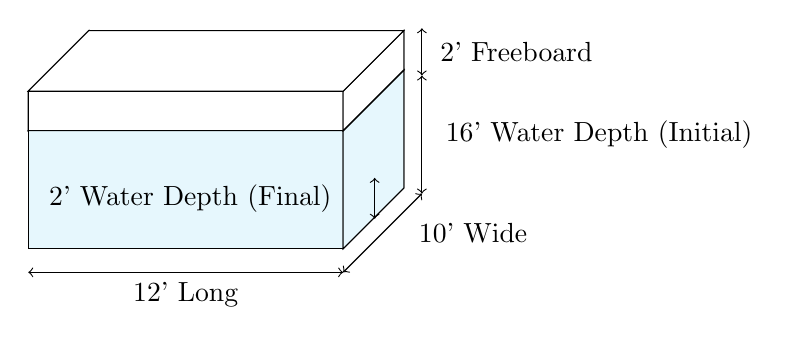
\begin{tikzpicture}

\pgfmathsetmacro{\cubexx}{4}
\pgfmathsetmacro{\cubeyy}{1.5}
\pgfmathsetmacro{\cubezz}{2}
\pgfmathsetmacro{\cubex}{4}
\pgfmathsetmacro{\cubey}{0.5}
\pgfmathsetmacro{\cubez}{2}
\pgfmathsetmacro{\cubexxx}{4}
\pgfmathsetmacro{\cubeyyy}{4}
\filldraw [fill=cyan!10!white, draw=black] (0,-\cubey,0) -- ++(-\cubexx,0,0) -- ++(0,-\cubeyy,0) -- ++(\cubexx,0,0) -- cycle ;
\filldraw [fill=cyan!0!white, draw=black] (0,-\cubey,0) -- ++(0,0,-\cubezz) -- ++(0,-\cubeyy,0) -- ++(0,0,\cubezz) -- cycle;
\filldraw [fill=cyan!10!white, draw=black] (0,-\cubey,0) -- ++(0,0,-\cubezz) -- ++(0,-\cubeyy,0) -- ++(0,0,\cubezz) -- cycle;
%\filldraw [fill=cyan!10!white, draw=black] (0,-\cubey,0) -- ++(-\cubexx,0,0) -- ++(0,0,-\cubezz) -- ++(\cubexx,0,0) -- cycle;
%%%\draw (0,-0.5,0) -- ++(-\cubex,0,0) -- ++(0,-\cubey,-\cubez) -- ++(\cubex,0,0) -- cycle;
\draw (-\cubex,0,0) -- ++(0,0,-\cubez) -- ++(0,-\cubey,0) -- ++(0,0,\cubez) -- cycle;
\draw (0,-\cubey,0) -- ++(-\cubex,0,0) -- ++(0,0,-\cubez) -- ++(\cubex,0,0) -- cycle;
\filldraw [fill=white, draw=black] (0,0,0) -- ++(-\cubex,0,0) -- ++(0,-\cubey,0) -- ++(\cubex,0,0) -- cycle ;
\filldraw [fill=white, draw=black] (0,0,0) -- ++(0,0,-\cubez) -- ++(0,-\cubey,0) -- ++(0,0,\cubez) -- cycle;
\filldraw [fill=white, draw=black] (0,0,0) -- ++(0,0,-\cubez) -- ++(0,-\cubey,0) -- ++(0,0,\cubez) -- cycle;
\filldraw [fill=white, draw=black] (0,0,0) -- ++(-\cubex,0,0) -- ++(0,0,-\cubez) -- ++(\cubex,0,0) -- cycle;

%\filldraw [fill=RoyalBlue!10!white, draw=black] (0,-1.5,0) -- ++(-\cubex,0,0) -- ++(0,-\cubey,0) -- ++(\cubex,0,0) -- cycle ;

%\filldraw [fill=RoyalBlue!10!white, draw=black] (0,-1.5,0) -- ++(0,0,-\cubez) -- ++(0,-\cubey,0) -- ++(0,0,\cubez) -- cycle;



%%\draw (0,-0.5,0) -- ++(-\cubex,0,0) -- ++(0,0,-\cubez) -- ++(\cubex,0,0) -- cycle;
%%\filldraw [fill=white, draw=black] (-\cubex,0,0) -- ++(0,0,-\cubez) -- ++(0,-\cubey,0) -- ++(0,0,\cubez) -- cycle;
%%\filldraw [fill=white, draw=black] (0,-\cubey,0) -- ++(-\cubex,0,0) -- ++(0,0,-\cubez) -- ++(\cubex,0,0) -- cycle ;

\draw [<->] (-4,-2.3) -- (0,-2.3) node [midway, below] {12' Long};
\draw [<->] (1,-1.3) -- (1,.2) node [midway, midway] {\hspace{4.5cm}16' Water Depth (Initial)};
\draw [<->] (0.4,-1.62) -- (0.4,-1.1) node [midway, midway] {\hspace{-4.8cm} 2' Water Depth (Final)};
\draw [<->] (1,.8) -- (1,.2) node [midway, midway] {\hspace{2.4cm}2' Freeboard};
\draw [<->] (1,-1.3) -- (0,-2.3) node [midway, midway] {\hspace{2.3cm}10' Wide};
\end{tikzpicture}\\
Volume to be pumped=$12 \enspace ft*10 \enspace ft *(16-2)\enspace ft=1,680ft^3$\\
\vspace{0.3cm}
$\implies \dfrac{1,680\cancel{ft^3}*7.48\dfrac{\cancel{gal}}{\cancel{ft^3}}}{600\dfrac{\cancel{gal}}{min}}=\boxed{21min}$

\item 1 MGD is pumped against a 14’ head.  What is the water Hp?  The pump mechanical efficiency is 85\%.  What is the brake horsepower?\\
\vspace{0.4cm}
water Hp = flow * head\\
\vspace{0.4cm}
$\dfrac{1,000,000 \enspace gal}{day}*\dfrac{day}{1440 \enspace min}*14 \enspace ft*\dfrac{Hp}{3,960 \enspace GPM-ft}=\boxed{Water \enspace Hp = 2.46 \enspace Hp}$\\
\vspace{0.4cm}
pump Hp = brake Hp * pump efficiency\\
\vspace{0.4cm}
$Brake \enspace Hp = \dfrac{2.46}{0.85}=\boxed{Brake \enspace Hp=2.89Hp}$\\

\vspace{0.4cm}

\item A 8 ft diameter cylindrical wetwell receives an average incoming flow if 135 gpm and is pumped down with a pump that delivers 450 gpm again a total dynamic head of 120 ft.  The pump is controlled using two floats; a stop float located at 2.5 ft and a start float located at 16 ft.  If the pump motor is rated at 88\% and the pump at 77\%, what is the monthly (30 days/month) for running this pump if power costs are \$0.11/Kwh?\\


\vspace{0.4cm}
When the pump is on, the volume of wetwell that will be pumped down with the 450 gpm pump and a 135 gpm flow to the wetwell:\\
\vspace{0.4cm}
$\dfrac{450 \enspace gal}{min}-\dfrac{135 \enspace gal}{min}=\dfrac{315 \enspace gal}{min}$\\
\vspace{0.4cm}
Minutes required to pump down the wetwell :\\
\vspace{0.4cm}
$0.785*8^2*(16-2.5)ft^3*\dfrac{7.48 \enspace gal}{ft^3}*\dfrac{min}{315 \enspace gal}=16.1 \enspace min$\\
\vspace{0.4cm}
Time to fill wetwell with pump off @135gal/min influent flow:
\\
\vspace{0.4cm}
$[0.785*8^2*(16-2.5)]ft^3*\dfrac{7.48 \enspace gal}{ft^3}*\dfrac{min}{135 \enspace gal}=37.6min$\\
\vspace{0.4cm}
\# of cycles per day:\\
\vspace{0.4cm}
$\dfrac{cycle}{(16.1+37.6) \enspace min}*\dfrac{1440 \enspace min}{day}=\dfrac{26.8 \enspace cycles}{day}$\\
\vspace{0.4cm}
\# of hrs pump operational:\\
\vspace{0.4cm}
$\dfrac{16.1 \enspace min}{cycle}*\dfrac{26.8 \enspace cycles}{day}*\dfrac{hrs}{60 \enspace min}=\dfrac{7.19 \enspace hours}{day}$\\
\vspace{0.4cm}
Monthly electrical cost:\\
\vspace{0.4cm}
$\dfrac{450 \enspace gpm*120 \enspace ft}{0.88*0.77}*\dfrac{Hp}{3,960 \enspace gpm-ft}*\dfrac{0.746 \enspace kW}{Hp}*\dfrac{7.19hrs}{day}*\dfrac{30 \enspace days}{month}*\dfrac{\$0.11}{kWh}=\boxed{\dfrac{\$356}{month}}$\\
\vspace{0.4cm}

\item A 6-year old pump motor is to be replaced at a net cost of \$15,800. The new motor, just like the old one, would run 65\% of the time. Both existing and replacement motors would operate at 125 output Hp. The existing motor efficiency is 86\% while the replacement motor would be guaranteed at 94\% efficiency. Electricity currently averages \$0.088 per kWh.\\
\vspace{0.4cm}
(a) Calculate the energy cost savings per year (to the nearest dollar) if the existing motor is replaced with the new motor (neglect any consideration of impact upon demand charges or interest on capital).\\
\vspace{0.4cm}
(b) What is payback period to the nearest tenth of a year.\\
\vspace{0.4cm}
Solution:\\
\vspace{0.4cm}
Calculate energy cost savings per year:\\
\vspace{0.4cm}
Input Hp for old motor:$\dfrac{125}{0.86}=145.35Hp$\\
\vspace{0.4cm}
Input Hp for old motor:$\dfrac{125}{0.94}=132.98Hp$\\
\vspace{0.4cm}
Energy cost savings:\\$(145.35-132.98)Hp*\dfrac{0.746 \enspace kW}{Hp}*\dfrac{(365*24*0.65)hrs}{yr}*\dfrac{\$0.088}{kWh}=\boxed{\dfrac{\$4,624}{yr}}$\\
\vspace{0.4cm}
Calculate payback:\\
\vspace{0.4cm}
$\$15,800*\dfrac{yr}{\$4,623.94}=\boxed{3.4yr}$


\item A flow of 200 gpm  is pumped against a total head of 4.0 feet. The pump is 78\% efficient and the motor' is 90\% efficient. Calculate the input Hp.\\
\vspace{0.4cm}
water Hp = flow * head\\
\vspace{0.2cm}
$200GPM*4ft*\dfrac{Hp}{3,960 GPM-ft}=0.2Hp$\\
\vspace{0.4cm}\includegraphics[scale=0.08]{PumpProblem}\\
water Hp=brake Hp*pump efficiency, and\\
brake Hp=input Hp*motor efficiency\\
Therefore, water Hp=input Hp*motor efficiency*pump efficiency\\
\vspace{0.4cm}
input Hp=$\dfrac{water \enspace Hp}{motor \enspace efficiency*pump \enspace efficiency}=\dfrac{0.2}{0.9*0.78}=\boxed{0.28Hp}$
\vspace{0.2cm}
\end{enumerate}






\newpage
\section*{Chapter Assessment}
\begin{tcolorbox}[breakable, enhanced,
colframe=blue!25,
colback=blue!10,
coltitle=blue!20!black,  
title= Chapter Assessment]

\begin{enumerate}
\item The chemical used for each day during a week is given below. Based on these data, what was the average lb/day chemical used during the week?\\

\begin{tabular}{|l|l|}
\hline
Monday & 92 lb/day\\
\hline
Tuesday & 93 lb/day \\
\hline
Wednesday & 98 lb/day\\
\hline
Thursday & 93 lb/day \\
\hline
Friday & 89 lb/day\\
\hline
Saturday & 93 lb/day \\
\hline
Sunday & 97 lb/day\\
\hline
\end{tabular}

\item The average day winter demand of a community is 14,500 gallons. If the summer demand is estimated to be $72 \%$ greater than the winter, what is the estimated summer demand? 


\item A 60-foot diameter tank contains 422,000 gallons of water. Calculate the height of water in the storage tank.

\item How much paint will it take for a single coat of the top and sidewalls of the storage tank that is 100-feet in diameter and 30-feet tall, if one gallon of paint covers 200 square feet?\\

\item A tank has a diameter of 60 feet with an overflow depth at 44 feet. The current water level is 16 feet. Water is flowing into the tank at a rate of 250 gallons per minute. At this rate, how many days will it take to fill the tank to the overflow?

\item A rectangular channel 3 ft. wide contains water 2 ft. deep flowing at a velocity of 1.5 fps.
What is the flow rate in cfs?

\item On an average, 2 inches of grit is collected and removed every day in a 2.2 feet wide, 205 feet long grit channel.  Knowing the average flow through that grit channel is 10 MGD calculate the rate of grit collection in ft$^3$/MG\\


\item A clarifier has a TSS removal efficiency of 50\%.  If the influent TSS concentration is 220 mg/L, how many lbs/day of TSS are removed if the flow is 10 MGD.  Also, how many cu. ft of sludge is pumped if the sludge has a TS concentration of 5\%.\\


\item What is the surface loading rate (gal/(day-sq.ft) of a 15 MGD flow in a 105 ft diameter primary sedimentation tank operating at water depth of 20 ft.\\

\item  A 12 MGD primary clarifier effluent flow is fed to a trickling filter. If the total flow to the trickling filter including the recirculated flow is 17 MGD, what is the recirculation ratio? \\

\item The flow to a pond is 7.2MGD. If the pond diameter is 350 ft and the BOD in the pond influent is 170mg/L, what is the organic loading to this pond in lbs BOD/day/acre?

\item How deep must a 60 acre facultative pond be operated in order to have a detention time of 45 days. Flow to the pond is 2.0 MGD. 

\item In an aeration tank, the MLSS is 2500 mg/l and recorded 30-minute settling test for a 1-litre MLSS samples indicates 230 ml of settled solids. What is the sludge volume index?

\item The desired F/M ratio is .35lbs BOD/day/lb MLVSS.  If 2,100 lbs of BOD enter the aerator daily, how many lbs of MLVSS should be maintained in the aeration tank? \\ 

\item Given the following data, calculate the mean cell residence time (MCRT)\\
DATA: \\
Influent flow= 35 MGD\\
MLSS = 2850 mg/L\\
Waste sludge flow = 0.08 MGD\\
Total secondary system volume= 20 MG\\
Waste activated sludge suspended solids conc. = 6000 mg/L\\
Final effluent suspended solids = 25 mg/L \\

\item 42,000 gallons of 6\% sludge containing 67\% volatile matter is pumped to the digester.  The digester reduces the volatile matter by 52\%.  What volume of sludge in gallons containing 5\% solids remains after digestion? 

\item How much gas is produced in the above digester in $ft^3$/day if the digested sludge contains 2.5\% total solids of which 59\% is volatile solids and the gas production rate is 14 $ft^3$/lb VS destroyed?\\

\item A belt press is used for dewatering 70 GPM digested sludge containing 3\% TS, seven hours per day.  At the end of the day it produces 24 $yd^3$ of 16\% TS \enspace biosolids @ 65 lbs/$ft^3$ density.  What is the percent belt press solids recovery?\\

\item Calculate the air required (SCFM) to meet a 0.04 lb air:lb feed solids ratio for a 100 GPM WAS flow with a solids content of 6500mg/l? Assume 0.08 lbs air/SCF air.\\

\item Calculate how many pounds per day of chlorine should be used to maintain a dosage of 12 mg/l at a 5.0 MGD flow.\\

\item The operator at a 1.5 MGD conventional activated sludge plant is considering using either HTH or sodium hypochlorite as an alternative to chlorine gas. Currently chlorine is being dosed at 15 mg/L in order to achieve a residual of 3.0 mg/L. Using the data provided below calculate the daily cost for chlorine, HTH, and sodium hypochlorite (NaOCl) (Sp.Gravity 1.21).
 
Chlorine $\rightarrow$ 0.15 \$/lb\\
HTH (70\% available chlorine) $\rightarrow$ 0.25 \$/lb\\
NaOCl (15\% available chlorine) $\rightarrow$ 0.35 \$/gal 


\item Liquid alum (49\% alum, sp. gravity 1.32, \$1.85/gal)) is being used to remove phosphorus from a 600,000 gpd activated sludge effluent. Two hundred milligrams per liter (200 mg/L) of alum, $Al_2(S0_4)_3.14H_20$, is required to give adequate removal of the phosphorus in this effluent. Calculate the daily cost of liquid alum needed to remove phosphorus. [Formula Weights: Al =27, $Al_2(S0_4)_3.14H_20$ =594]\\

\item Find the brake horsepower for a pump given the following information: Total Dynamic Head $=75$ feet, Pump Rate $=150$ gpm, Pump Efficiency $=90 \%$, Motor Efficiency $=85 \%$

\end{enumerate}
\end{tcolorbox}

















\chapterimage{FutureChapterImage2.png}
\chapter{Wastewater Treatment - Future}

\section{Water Resource Recovery Facility - WRRF}\index{Water Resource Recovery Facility - WRRF}
\begin{itemize}
\item Originally, the function of a wastewater treatment plant was collection, treatment and disposal which was driven solely by the need to reduce human disease and to protect the environment.
\item It was soon realized that wastewater contains valuable elements like organic matter, phosphorus, nitrogen, rare metals and thermal energy
\item The scope of wastewater treatment has now evolved to encompass recovering valuable resources contained in the wastewater.
\item The wastewater treatment plant is now known as a water resource recovery facility (WRRF). 
\item This change reflects the new focus on the products and benefits of treatment rather than its original and only objective - treating water for sanitation.
\item The WRRF is being adapted into the concept of the circular economy in which products, materials (and raw materials) remain in the economy for as long as possible, and waste is treated as secondary raw materials that can be recycled to process and re-used.  This distinguishes it from a linear economy which is based on the: "take-make-use-dispose" system, in which waste is usually the last stage of the product life cycle.

\end{itemize}

\subsection{Water}\index{Water}
\begin{itemize}
\item Municipal wastewater reuse offers the potential to significantly increase the nation’s total available water resources. Of the 32 billion gallons of treated wastewater discharged nationally, approximately 12 billion gallons of treated wastewater is discharged each day to an ocean or estuary.
\item WRRF is key to the use of treated wastewater, or “reclaimed” water, for beneficial purposes such as drinking, irrigation, or industrial uses—is one option that has helped some communities significantly expand their water supplies.
\item Wastewater can be treated to various qualities to satisfy demand from different sectors, including industry and agriculture. It can be used to maintain the environmental flow, or even reused as drinking water. 
\item Wastewater treatment is one solution to the water scarcity issue, and also to the problem of water security, freeing water resources for other uses or for preservation.
\end{itemize}




\subsection{Energy}\index{Energy}
\begin{itemize}
\item In the US, municipal wastewater treatment plants consume 30 terawatt-hours per year of electricity which is about 0.1\% of the total electrical consumption.  
\item WRRFs have the potential to be energy neutral or even net energy producers through comprehensive energy management approaches, incorporating efficient practices, and generating renewable energy from their by-products, such as biosolids.

\item By making the treatment processes more energy efficient and through the recovery of chemical or calorific energy in the wastewater play a key role in reducing the carbon foot print of the WRRF. 

\item Given the amount of chemical or calorific energy contained in wastewater, the goal is for the WRRFs to be energy neutral or even energy positive - which is to produce same or more energy than the energy needed for treatment.
\end{itemize}


\subsection{Nutrients}\index{Nutrients}
\begin{itemize}
\item Nutrient recovery is the practice of recovering nutrients such as nitrogen and phosphorus from used water streams that would otherwise be discarded/disposed and converting them into fertilizer used for ecological and agricultural purposes. 
\item Phosphate used in fertilizers is manufactured from phosphate rock using a very environmentally detrimental mining process.  Recovery/reuse of phosphate from wastewater mitigates dependence on this mined mineral.
\end{itemize} 
Nutrient recovery at a WRRF is accomplished using one of following two methods:
\begin{enumerate}[1.] 
\item By precipitating phosphorous as struvite crystals using a dedicated reactor. The struvite crystals are collected and resold as fertilizer which has a resale value ranging from \$100-\$600 per dry ton.  Benefits of this method include:
\begin{itemize}
\item Generation of revenue from the fertilizer produced
\item Reduces fouling of equipment due to precipitation of struvite formed during the solids treatment process
\item Allows for meeting NPDES nutrients discharge limits
\end{itemize}
\item Nutrient recovery can also be achieved through the land application of biosolids. Benefits of land application of biosolids include:
\begin{itemize}
\item Provide primary nutrients - nitrogen and phosphorous and secondary nutrients such as calcium, iron, magnesium and zinc for crops.
\item The organic carbon and organic matter in the biosolids help build better soils. 
\item Allows for sequestering carbon in the soil.
\end{itemize}
\end{enumerate}


\section{Challenges to WRRF}\index{Challenges to WRRF}

\subsection{Constituents of Emerging Concern}\index{Constituents of Emerging Concern}
\begin{itemize}
\item Constituents of Emerging Concern (CECs) include a variety of substances such as medicines, personal care products, flame retardants, algal toxins, micorplastics, and many others that are not currently federally regulated but known to occur in water.
\item Some of these CECs, incuding hormones, PFAS, and endocrine disruptors are known to pose health risks to humans and aquatic life.
\item Although some CECs that reach WRRFs are destroyed through wastewater treatment and solids processing, some recalcitrant microconstituents and their metabolites may pass through the treatment process intact and may end up in the effluent or biosolids. 
\item Both, the dose (concentration) of the CEC present and frequency/duration of exposure is important for interpreting possible risk to ecological and human health.
\item The CECs move in their complex cycling through surface and groundwaters across the planet - from potable water to wastewater and viceversa as potable water is converted into wastewater followed by uptake of the treated wastewater by the potable water supply system through groundwater contaminated by the percolation of these CECs in land applied wastewater biosolids or through the CECs in the treated wastewater discharge to surface water such as a lake or river.
\item The CECs concentrations in the plant influent range typically in nano-g/L to micro-g/L , in effluent from non-detect to nano-g/L, and in biosolids the concentrations vary from micro-g/kg to mg/kg.
\end{itemize}


\subsection{Decentralized and Distributed Systems}\index{Decentralized and Distributed Systems}
\begin{itemize}
\item To make the wastewater treatment systems more sustainable and to overcome the issues of a centralized system where wastewater is collected from various areas and cities in urban areas and conveyed to a centrally located plant for treatment, it is imperative to consider 
\item \textbf{Distributed systems} are in different geographical locations, but are linked to a central system either physically, or by management. \textbf{Decentralized systems} can be located in a different geographical location, but are not linked physically, or are not managed under the umbrella of a centralized system.
\item Through the selection of correct locations and appropriate technologies, distributed or decentralized systems can:
\begin{itemize}
\item Provide environmental benefits, such as nutrient and pathogen removal
\item Provide water for direct potable reuse and non-potable water in both rural and urban settings for purposes such as flushing, cooling and heating, landscaping, and subsurface irrigation drip.
\end{itemize}
\end{itemize}


\subsection{Climate Change}\index{Climate Change} 
\begin{itemize}
\item Climate change has directly impacted water resources by altering precipitation patterns, severe drought and floods, snowpack amount, elevation, stream flow, and rising sea levels. 
\item This has created a direct need for utilities to manage local water resources to lessen the potential impact of climate change. 
\item By increasing water reuse, developing resiliency and other actions, WRRFs can be a leader in fighting and preparing for climate change effects.
\item Driven largely by climate change factors, lower carbon footprint - the amount of carbon dioxide and other carbon compounds emitted due to the consumption of fossil fuels (energy), and lower energy demands are now being factored in when assessing wastewater treatment options.
\end{itemize}
\newpage
\begin{center}
\includegraphics[scale=0.55]{WBWasteWaterResourceinfographic.png}\\
\emph{Source:  Waste to Resource - World Bank}\\
\end{center}









\input{BassettWWCareers.tex}
\input{BassettWWGlossary.tex}  
\part{Appendix}
\chapterimage{AppendixChapterImage} % Chapter heading image

\appendix

\renewcommand{\chaptername}{Appendix A: } % Change the chapter name to Appendix, i.e. "Appendix A: Title", instead of "Chapter A: Title" in the headers

\vfill

\appendix
\chapterimage{AppendixChapterImage} % Chapter heading image


\chapter{Treatment Exam - ROK}\label{appendix:Treatment Exam - ROK}
\includepdf[pages={1-11}]{RangeofKnowledgeforTreatmentExam}

\chapter{Distribution Exam - ROK}\label{appendix:Distribution Exam - ROK}
\includepdf[pages={1-14}]{RangeofKnowledgeforDistributionExam}

\chapter{Wastewater Exams}\label{appendix:Wastewater Exams}
\includepdf[pages={1-5}]{WWExams}

\chapter{Water Treatment Facilities Classification}\label{appendix:Water Treatment Facilities Classification}
\includepdf[pages={1-2}]{CCR64413.1}

\chapter{SDS Content - OSHA Guidance}\label{appendix:SDS Content - OSHA Guidance}
\includepdf[pages=-]{oshasds.pdf}

\chapter{Sample SDS}\label{appendix:Sample SDS}
\includepdf[pages=-]{anhydammoniasds.pdf}
\end{document}
